%%%%%%%%%%%%%%%%%%%%%%%%%%%%%%%%%%%%%%%%%
%  My documentation report
%  Objetive: Explain what I did and how, so someone can continue with the investigation
%
% Important note:
% Chapter heading images should have a 2:1 width:height ratio,
% e.g. 920px width and 460px height.
%
%%%%%%%%%%%%%%%%%%%%%%%%%%%%%%%%%%%%%%%%%

%----------------------------------------------------------------------------------------
% PACKAGES AND OTHER DOCUMENT CONFIGURATIONS
%----------------------------------------------------------------------------------------

\documentclass[11pt]{book}
% \documentclass[11pt,draft]{book} % Use to see overflows
\usepackage[
top=3cm,
bottom=3cm,
left=3.2cm,
right=3.2cm,
headsep=10pt,
letterpaper,
% showframe
]{geometry} % Page margins
%%%%%%%%%%%%%%%%%%%%%%%%%%%%%%%%%%%%%%%%%
% The Legrand Orange Book
% Structural Definitions File
% Version 2.0 (9/2/15)
%
% Original author:
% Mathias Legrand (legrand.mathias@gmail.com) with modifications by:
% Vel (vel@latextemplates.com)
% 
% This file has been downloaded from:
% http://www.LaTeXTemplates.com
%
% License:
% CC BY-NC-SA 3.0 (http://creativecommons.org/licenses/by-nc-sa/3.0/)
%
%%%%%%%%%%%%%%%%%%%%%%%%%%%%%%%%%%%%%%%%%

%----------------------------------------------------------------------------------------
%	VARIOUS REQUIRED PACKAGES AND CONFIGURATIONS
%----------------------------------------------------------------------------------------

\usepackage[top=3cm,bottom=3cm,left=3cm,right=3cm,headsep=10pt,a4paper]{geometry} % Page margins

\usepackage{graphicx} % Required for including pictures
\graphicspath{{Pictures/}} % Specifies the directory where pictures are stored

\usepackage{lipsum} % Inserts dummy text

\usepackage{tikz} % Required for drawing custom shapes

\usepackage[english]{babel} % English language/hyphenation

\usepackage{enumitem} % Customize lists
\setlist{nolistsep} % Reduce spacing between bullet points and numbered lists

\usepackage{booktabs} % Required for nicer horizontal rules in tables

\usepackage{xcolor} % Required for specifying colors by name
% \definecolor{ocre}{RGB}{243,102,25} % Orange
% \definecolor{ocre}{RGB}{0,0,128} % Navy
% \definecolor{ocre}{RGB}{65,105,225} % Royal Blue
\definecolor{ocre}{RGB}{255,69,0} % Orange Red

%----------------------------------------------------------------------------------------
%	FONTS
%----------------------------------------------------------------------------------------

% \usepackage{avant} % Use the Avantgarde font for headings
% \usepackage{times} % Use the Times font for headings
% \usepackage{mathptmx} % Use the Adobe Times Roman as the default text font together with math symbols from the Sym­bol, Chancery and Com­puter Modern fonts
\usepackage{libertine}
\usepackage{tgcursor}

\usepackage{microtype} % Slightly tweak font spacing for aesthetics
\usepackage[utf8]{inputenc} % Required for including letters with accents
\usepackage[T1]{fontenc} % Use 8-bit encoding that has 256 glyphs

%----------------------------------------------------------------------------------------
%	BIBLIOGRAPHY
%----------------------------------------------------------------------------------------

% \usepackage[style=alphabetic,citestyle=numeric,sorting=nyt,sortcites=true,autopunct=true,babel=hyphen,hyperref=true,abbreviate=false,backref=true,backend=biber]{biblatex}
% \usepackage{biblatex}
% \addbibresource{allrefs.bib} % BibTeX bibliography file
% \defbibheading{bibempty}{}

\usepackage{calc} % For simpler calculation - used for spacing the index letter headings correctly

%----------------------------------------------------------------------------------------
%	MAIN TABLE OF CONTENTS
%----------------------------------------------------------------------------------------

\usepackage{titletoc} % Required for manipulating the table of contents

\contentsmargin{0cm} % Removes the default margin

% Part text styling
\titlecontents{part}[0cm]
{\addvspace{20pt}\centering\large\bfseries}
{}
{}
{}

% Chapter text styling
\titlecontents{chapter}[1.25cm] % Indentation
{\addvspace{12pt}\large\sffamily\bfseries} % Spacing and font options for chapters
{\color{ocre!60}\contentslabel[\Large\thecontentslabel]{1.25cm}\color{ocre}} % Chapter number
{\color{ocre}}  
{\color{ocre!60}\normalsize\;\titlerule*[.5pc]{.}\;\thecontentspage} % Page number

% Section text styling
\titlecontents{section}[1.25cm] % Indentation
{\addvspace{3pt}\sffamily\bfseries} % Spacing and font options for sections
{\contentslabel[\thecontentslabel]{1.25cm}} % Section number
{}
{\hfill\color{black}\thecontentspage} % Page number
[]

% Subsection text styling
\titlecontents{subsection}[1.25cm] % Indentation
{\addvspace{1pt}\sffamily\small} % Spacing and font options for subsections
{\contentslabel[\thecontentslabel]{1.25cm}} % Subsection number
{}
{\ \titlerule*[.5pc]{.}\;\thecontentspage} % Page number
[]

% List of figures
\titlecontents{figure}[0em]
{\addvspace{-5pt}\sffamily}
{\thecontentslabel\hspace*{1em}}
{}
{\ \titlerule*[.5pc]{.}\;\thecontentspage}
[]

% List of tables
\titlecontents{table}[0em]
{\addvspace{-5pt}\sffamily}
{\thecontentslabel\hspace*{1em}}
{}
{\ \titlerule*[.5pc]{.}\;\thecontentspage}
[]

%----------------------------------------------------------------------------------------
%	MINI TABLE OF CONTENTS IN PART HEADS
%----------------------------------------------------------------------------------------

% Chapter text styling
\titlecontents{lchapter}[0em] % Indenting
{\addvspace{15pt}\large\sffamily\bfseries} % Spacing and font options for chapters
{\color{ocre}\contentslabel[\Large\thecontentslabel]{1.25cm}\color{ocre}} % Chapter number
{}  
{\color{ocre}\normalsize\sffamily\bfseries\;\titlerule*[.5pc]{.}\;\thecontentspage} % Page number

% Section text styling
\titlecontents{lsection}[0em] % Indenting
{\sffamily\small} % Spacing and font options for sections
{\contentslabel[\thecontentslabel]{1.25cm}} % Section number
{}
{}

% Subsection text styling
\titlecontents{lsubsection}[.5em] % Indentation
{\normalfont\footnotesize\sffamily} % Font settings
{}
{}
{}

%----------------------------------------------------------------------------------------
%	PAGE HEADERS
%----------------------------------------------------------------------------------------

\usepackage{fancyhdr} % Required for header and footer configuration

\pagestyle{fancy}
\renewcommand{\chaptermark}[1]{\markboth{\sffamily\normalsize\bfseries\chaptername\ \thechapter.\ #1}{}} % Chapter text font settings
\renewcommand{\sectionmark}[1]{\markright{\sffamily\normalsize\thesection\hspace{5pt}#1}{}} % Section text font settings
\fancyhf{} \fancyhead[LE,RO]{\sffamily\normalsize\thepage} % Font setting for the page number in the header
\fancyhead[LO]{\rightmark} % Print the nearest section name on the left side of odd pages
\fancyhead[RE]{\leftmark} % Print the current chapter name on the right side of even pages
\renewcommand{\headrulewidth}{0.5pt} % Width of the rule under the header
\addtolength{\headheight}{2.5pt} % Increase the spacing around the header slightly
\renewcommand{\footrulewidth}{0pt} % Removes the rule in the footer
\fancypagestyle{plain}{\fancyhead{}\renewcommand{\headrulewidth}{0pt}} % Style for when a plain pagestyle is specified

% Removes the header from odd empty pages at the end of chapters
\makeatletter
\renewcommand{\cleardoublepage}{
\clearpage\ifodd\c@page\else
\hbox{}
\vspace*{\fill}
\thispagestyle{empty}
\newpage
\fi}

%----------------------------------------------------------------------------------------
%	THEOREM STYLES
%----------------------------------------------------------------------------------------

\usepackage{amsmath,amsfonts,amssymb,amsthm} % For math equations, theorems, symbols, etc

\newcommand{\intoo}[2]{\mathopen{]}#1\,;#2\mathclose{[}}
\newcommand{\ud}{\mathop{\mathrm{{}d}}\mathopen{}}
\newcommand{\intff}[2]{\mathopen{[}#1\,;#2\mathclose{]}}
\newtheorem{notation}{Notation}[chapter]

% Boxed/framed environments
\newtheoremstyle{ocrenumbox}% % Theorem style name
{0pt}% Space above
{0pt}% Space below
{\normalfont}% % Body font
{}% Indent amount
{\small\bf\sffamily\color{ocre}}% % Theorem head font
{\;}% Punctuation after theorem head
{0.25em}% Space after theorem head
{\small\sffamily\color{ocre}\thmname{#1}\nobreakspace\thmnumber{\@ifnotempty{#1}{}\@upn{#2}}% Theorem text (e.g. Theorem 2.1)
\thmnote{\nobreakspace\the\thm@notefont\sffamily\bfseries\color{black}---\nobreakspace#3.}} % Optional theorem note
\renewcommand{\qedsymbol}{$\blacksquare$}% Optional qed square

\newtheoremstyle{blacknumex}% Theorem style name
{5pt}% Space above
{5pt}% Space below
{\normalfont}% Body font
{} % Indent amount
{\small\bf\sffamily}% Theorem head font
{\;}% Punctuation after theorem head
{0.25em}% Space after theorem head
{\small\sffamily{\tiny\ensuremath{\blacksquare}}\nobreakspace\thmname{#1}\nobreakspace\thmnumber{\@ifnotempty{#1}{}\@upn{#2}}% Theorem text (e.g. Theorem 2.1)
\thmnote{\nobreakspace\the\thm@notefont\sffamily\bfseries---\nobreakspace#3.}}% Optional theorem note

\newtheoremstyle{blacknumbox} % Theorem style name
{0pt}% Space above
{0pt}% Space below
{\normalfont}% Body font
{}% Indent amount
{\small\bf\sffamily}% Theorem head font
{\;}% Punctuation after theorem head
{0.25em}% Space after theorem head
{\small\sffamily\thmname{#1}\nobreakspace\thmnumber{\@ifnotempty{#1}{}\@upn{#2}}% Theorem text (e.g. Theorem 2.1)
\thmnote{\nobreakspace\the\thm@notefont\sffamily\bfseries---\nobreakspace#3.}}% Optional theorem note

% Non-boxed/non-framed environments
\newtheoremstyle{ocrenum}% % Theorem style name
{5pt}% Space above
{5pt}% Space below
{\normalfont}% % Body font
{}% Indent amount
{\small\bf\sffamily\color{ocre}}% % Theorem head font
{\;}% Punctuation after theorem head
{0.25em}% Space after theorem head
{\small\sffamily\color{ocre}\thmname{#1}\nobreakspace\thmnumber{\@ifnotempty{#1}{}\@upn{#2}}% Theorem text (e.g. Theorem 2.1)
\thmnote{\nobreakspace\the\thm@notefont\sffamily\bfseries\color{black}---\nobreakspace#3.}} % Optional theorem note
\renewcommand{\qedsymbol}{$\blacksquare$}% Optional qed square
\makeatother

% Defines the theorem text style for each type of theorem to one of the three styles above
\newcounter{dummy} 
\numberwithin{dummy}{section}
\theoremstyle{ocrenumbox}
\newtheorem{theoremeT}[dummy]{Theorem}
\newtheorem{problem}{Problem}[chapter]
\newtheorem{exerciseT}{Exercise}[chapter]
\theoremstyle{blacknumex}
\newtheorem{exampleT}{Example}[chapter]
\theoremstyle{blacknumbox}
\newtheorem{vocabulary}{Vocabulary}[chapter]
\newtheorem{definitionT}{Definition}[section]
\newtheorem{corollaryT}[dummy]{Corollary}
\theoremstyle{ocrenum}
\newtheorem{proposition}[dummy]{Proposition}

%----------------------------------------------------------------------------------------
%	DEFINITION OF COLORED BOXES
%----------------------------------------------------------------------------------------

\RequirePackage[framemethod=default]{mdframed} % Required for creating the theorem, definition, exercise and corollary boxes

% Theorem box
\newmdenv[skipabove=7pt,
skipbelow=7pt,
backgroundcolor=black!5,
linecolor=ocre,
innerleftmargin=5pt,
innerrightmargin=5pt,
innertopmargin=5pt,
leftmargin=0cm,
rightmargin=0cm,
innerbottommargin=5pt]{tBox}

% Exercise box	  
\newmdenv[skipabove=7pt,
skipbelow=7pt,
rightline=false,
leftline=true,
topline=false,
bottomline=false,
backgroundcolor=ocre!10,
linecolor=ocre,
innerleftmargin=5pt,
innerrightmargin=5pt,
innertopmargin=5pt,
innerbottommargin=5pt,
leftmargin=0cm,
rightmargin=0cm,
linewidth=4pt]{eBox}	

% Definition box
\newmdenv[skipabove=7pt,
skipbelow=7pt,
rightline=false,
leftline=true,
topline=false,
bottomline=false,
linecolor=ocre,
innerleftmargin=5pt,
innerrightmargin=5pt,
innertopmargin=0pt,
leftmargin=0cm,
rightmargin=0cm,
linewidth=4pt,
innerbottommargin=0pt]{dBox}	

% Corollary box
\newmdenv[skipabove=7pt,
skipbelow=7pt,
rightline=false,
leftline=true,
topline=false,
bottomline=false,
linecolor=gray,
backgroundcolor=black!5,
innerleftmargin=5pt,
innerrightmargin=5pt,
innertopmargin=5pt,
leftmargin=0cm,
rightmargin=0cm,
linewidth=4pt,
innerbottommargin=5pt]{cBox}

% Creates an environment for each type of theorem and assigns it a theorem text style from the "Theorem Styles" section above and a colored box from above
\newenvironment{theorem}{\begin{tBox}\begin{theoremeT}}{\end{theoremeT}\end{tBox}}
\newenvironment{exercise}{\begin{eBox}\begin{exerciseT}}{\hfill{\color{ocre}\tiny\ensuremath{\blacksquare}}\end{exerciseT}\end{eBox}}				  
\newenvironment{definition}{\begin{dBox}\begin{definitionT}}{\end{definitionT}\end{dBox}}	
\newenvironment{example}{\begin{exampleT}}{\hfill{\tiny\ensuremath{\blacksquare}}\end{exampleT}}		
\newenvironment{corollary}{\begin{cBox}\begin{corollaryT}}{\end{corollaryT}\end{cBox}}	

%----------------------------------------------------------------------------------------
%	REMARK ENVIRONMENT
%----------------------------------------------------------------------------------------

\newenvironment{remark}{\par\vspace{10pt}\small % Vertical white space above the remark and smaller font size
\begin{list}{}{
\leftmargin=35pt % Indentation on the left
\rightmargin=25pt}\item\ignorespaces % Indentation on the right
\makebox[-2.5pt]{\begin{tikzpicture}[overlay]
\node[draw=ocre!60,line width=1pt,circle,fill=ocre!25,font=\sffamily\bfseries,inner sep=2pt,outer sep=0pt] at (-15pt,0pt){\textcolor{ocre}{R}};\end{tikzpicture}} % Orange R in a circle
\advance\baselineskip -1pt}{\end{list}\vskip5pt} % Tighter line spacing and white space after remark

%----------------------------------------------------------------------------------------
%	SECTION NUMBERING IN THE MARGIN
%----------------------------------------------------------------------------------------

\makeatletter
\renewcommand{\@seccntformat}[1]{\llap{\textcolor{ocre}{\csname the#1\endcsname}\hspace{1em}}}                    
\renewcommand{\section}{\@startsection{section}{1}{\z@}
{-4ex \@plus -1ex \@minus -.4ex}
{1ex \@plus.2ex }
{\normalfont\large\sffamily\bfseries}}
\renewcommand{\subsection}{\@startsection {subsection}{2}{\z@}
{-3ex \@plus -0.1ex \@minus -.4ex}
{0.5ex \@plus.2ex }
{\normalfont\sffamily\bfseries}}
\renewcommand{\subsubsection}{\@startsection {subsubsection}{3}{\z@}
{-2ex \@plus -0.1ex \@minus -.2ex}
{.2ex \@plus.2ex }
{\normalfont\small\sffamily\bfseries}}                        
\renewcommand\paragraph{\@startsection{paragraph}{4}{\z@}
{-2ex \@plus-.2ex \@minus .2ex}
{.1ex}
{\normalfont\small\sffamily\bfseries}}

%----------------------------------------------------------------------------------------
%	PART HEADINGS
%----------------------------------------------------------------------------------------

% numbered part in the table of contents
\newcommand{\@mypartnumtocformat}[2]{%
\setlength\fboxsep{0pt}%
\noindent\colorbox{ocre!20}{\strut\parbox[c][.7cm]{\ecart}{\color{ocre!70}\Large\sffamily\bfseries\centering#1}}\hskip\esp\colorbox{ocre!40}{\strut\parbox[c][.7cm]{\linewidth-\ecart-\esp}{\Large\sffamily\centering#2}}}%
%%%%%%%%%%%%%%%%%%%%%%%%%%%%%%%%%%
% unnumbered part in the table of contents
\newcommand{\@myparttocformat}[1]{%
\setlength\fboxsep{0pt}%
\noindent\colorbox{ocre!40}{\strut\parbox[c][.7cm]{\linewidth}{\Large\sffamily\centering#1}}}%
%%%%%%%%%%%%%%%%%%%%%%%%%%%%%%%%%%
\newlength\esp
\setlength\esp{4pt}
\newlength\ecart
\setlength\ecart{1.2cm-\esp}
\newcommand{\thepartimage}{}%
\newcommand{\partimage}[1]{\renewcommand{\thepartimage}{#1}}%
\def\@part[#1]#2{%
\ifnum \c@secnumdepth >-2\relax%
\refstepcounter{part}%
\addcontentsline{toc}{part}{\texorpdfstring{\protect\@mypartnumtocformat{\thepart}{#1}}{\partname~\thepart\ ---\ #1}}
\else%
\addcontentsline{toc}{part}{\texorpdfstring{\protect\@myparttocformat{#1}}{#1}}%
\fi%
\startcontents%
\markboth{}{}%
{\thispagestyle{empty}%
\begin{tikzpicture}[remember picture,overlay]%
\node at (current page.north west){\begin{tikzpicture}[remember picture,overlay]%	
\fill[ocre!20](0cm,0cm) rectangle (\paperwidth,-\paperheight);
\node[anchor=north] at (4cm,-3.25cm){\color{ocre!40}\fontsize{220}{100}\sffamily\bfseries\@Roman\c@part}; 
\node[anchor=south east] at (\paperwidth-1cm,-\paperheight+1cm){\parbox[t][][t]{8.5cm}{
\printcontents{l}{0}{\setcounter{tocdepth}{1}}%
}};
\node[anchor=north east] at (\paperwidth-1.5cm,-3.25cm){\parbox[t][][t]{15cm}{\strut\raggedleft\color{white}\fontsize{30}{30}\sffamily\bfseries#2}};
\end{tikzpicture}};
\end{tikzpicture}}%
\@endpart}
\def\@spart#1{%
\startcontents%
\phantomsection
{\thispagestyle{empty}%
\begin{tikzpicture}[remember picture,overlay]%
\node at (current page.north west){\begin{tikzpicture}[remember picture,overlay]%	
\fill[ocre!20](0cm,0cm) rectangle (\paperwidth,-\paperheight);
\node[anchor=north east] at (\paperwidth-1.5cm,-3.25cm){\parbox[t][][t]{15cm}{\strut\raggedleft\color{white}\fontsize{30}{30}\sffamily\bfseries#1}};
\end{tikzpicture}};
\end{tikzpicture}}
\addcontentsline{toc}{part}{\texorpdfstring{%
\setlength\fboxsep{0pt}%
\noindent\protect\colorbox{ocre!40}{\strut\protect\parbox[c][.7cm]{\linewidth}{\Large\sffamily\protect\centering #1\quad\mbox{}}}}{#1}}%
\@endpart}
\def\@endpart{\vfil\newpage
\if@twoside
\if@openright
\null
\thispagestyle{empty}%
\newpage
\fi
\fi
\if@tempswa
\twocolumn
\fi}

%----------------------------------------------------------------------------------------
%	CHAPTER HEADINGS
%----------------------------------------------------------------------------------------

% A switch to conditionally include a picture, implemented by  Christian Hupfer
\newif\ifusechapterimage
\usechapterimagetrue
\newcommand{\thechapterimage}{}%
\newcommand{\chapterimage}[1]{\ifusechapterimage\renewcommand{\thechapterimage}{#1}\fi}%
\def\@makechapterhead#1{%
{\parindent \z@ \raggedright \normalfont
\ifnum \c@secnumdepth >\m@ne
\if@mainmatter
\begin{tikzpicture}[remember picture,overlay]
\node at (current page.north west)
{\begin{tikzpicture}[remember picture,overlay]
\node[anchor=north west,inner sep=0pt] at (0,0) {\ifusechapterimage\includegraphics[width=\paperwidth]{\thechapterimage}\fi};
\draw[anchor=west] (\Gm@lmargin,-9cm) node [line width=2pt,rounded corners=15pt,draw=ocre,fill=white,fill opacity=0.5,inner sep=15pt]{\strut\makebox[22cm]{}};
\draw[anchor=west] (\Gm@lmargin+.3cm,-9cm) node {\huge\sffamily\bfseries\color{black}\thechapter. #1\strut};
\end{tikzpicture}};
\end{tikzpicture}
\else
\begin{tikzpicture}[remember picture,overlay]
\node at (current page.north west)
{\begin{tikzpicture}[remember picture,overlay]
\node[anchor=north west,inner sep=0pt] at (0,0) {\ifusechapterimage\includegraphics[width=\paperwidth]{\thechapterimage}\fi};
\draw[anchor=west] (\Gm@lmargin,-9cm) node [line width=2pt,rounded corners=15pt,draw=ocre,fill=white,fill opacity=0.5,inner sep=15pt]{\strut\makebox[22cm]{}};
\draw[anchor=west] (\Gm@lmargin+.3cm,-9cm) node {\huge\sffamily\bfseries\color{black}#1\strut};
\end{tikzpicture}};
\end{tikzpicture}
\fi\fi\par\vspace*{270\p@}}}

%-------------------------------------------

\def\@makeschapterhead#1{%
\begin{tikzpicture}[remember picture,overlay]
\node at (current page.north west)
{\begin{tikzpicture}[remember picture,overlay]
\node[anchor=north west,inner sep=0pt] at (0,0) {\ifusechapterimage\includegraphics[width=\paperwidth]{\thechapterimage}\fi};
\draw[anchor=west] (\Gm@lmargin,-9cm) node [line width=2pt,rounded corners=15pt,draw=ocre,fill=white,fill opacity=0.5,inner sep=15pt]{\strut\makebox[22cm]{}};
\draw[anchor=west] (\Gm@lmargin+.3cm,-9cm) node {\huge\sffamily\bfseries\color{black}#1\strut};
\end{tikzpicture}};
\end{tikzpicture}
\par\vspace*{270\p@}}
\makeatother

%----------------------------------------------------------------------------------------
%	HYPERLINKS IN THE DOCUMENTS
%----------------------------------------------------------------------------------------

\usepackage{hyperref}
\hypersetup{hidelinks,backref=true,pagebackref=true,hyperindex=true,colorlinks=false,breaklinks=true,urlcolor= ocre,bookmarks=true,bookmarksopen=false,pdftitle={LQCD on Intel Xeon Phi's},pdfauthor={Peter Labus}}
\usepackage{bookmark}
\bookmarksetup{
open,
numbered,
addtohook={%
\ifnum\bookmarkget{level}=0 % chapter
\bookmarksetup{bold}%
\fi
\ifnum\bookmarkget{level}=-1 % part
\bookmarksetup{color=ocre,bold}%
\fi
}
}
 % Insert the structure.tex file which contains
                  % the majority of the structure behind the template

%----------------------------------------------------------------------------------------
% MY PERSONAL INCLUDES AND STUFF
%----------------------------------------------------------------------------------------

\usepackage{color}
\usepackage{colortbl}
\usepackage{multirow}
\usepackage[makeroom]{cancel} % needed for xcancel

\usepackage{textcomp}
\usepackage{mathtools} % loads amsmath
\usepackage{amsfonts}
\usepackage{amssymb}
\usepackage{dsfont}
% \usepackage{bbold}

\usepackage{pifont}
\usepackage{nicefrac} % for \nicefrac macro giving nice fractions in exponent
\usepackage[font={small,it}]{caption}
\usepackage{footmisc}
\usepackage[super]{nth} % for 2nd, 3rd and so on
\usepackage{siunitx}
\usepackage{epstopdf}
\usepackage{array}
\setlength{\heavyrulewidth}{1.5pt}
\setlength{\abovetopsep}{4pt}
\usepackage{pdfpages}
\usepackage{emptypage}
\usepackage{stmaryrd}
\usepackage{setspace}
\usepackage[toc,page]{appendix}

% Packages for the bibliography
\usepackage{cite}
\usepackage{bibentry} % used to have a full inlined citation
\nobibliography*

% Packages and settings for dates
\usepackage[]{datetime}
\newdateformat{monthyeardate}{\monthname[\THEMONTH] \THEYEAR}
\newdateformat{dateall}{\THEDAY th \monthname[\THEMONTH] \THEYEAR}

%----------------------------------------------------------------------------------------
% TikZ & PGFPLOTS SETUP (FOR PLOTTING IN LATEX)
%----------------------------------------------------------------------------------------

\usepackage{tikz}
\usepackage{pgfplots}
\pgfplotsset{compat=newest}

\usetikzlibrary{patterns}
\usetikzlibrary{matrix}
\usetikzlibrary{positioning}
\usetikzlibrary{arrows}
\usetikzlibrary{fit}
\usetikzlibrary{math}
\usetikzlibrary{calc}
\usetikzlibrary{backgrounds}
\usetikzlibrary{decorations.pathmorphing}
\usetikzlibrary{decorations.markings}
\usetikzlibrary{pgfplots.groupplots}

\tikzset{
  midarrow/.style={draw, postaction={decorate},
  decoration={markings,mark=at position .55 with {\arrow[draw]{>}}}},
  midarrow-rev/.style={draw, postaction={decorate},
  decoration={markings,mark=at position .55 with {\arrow[draw]{<}}}},
  midarrow-dashed/.style={draw, dashed, postaction={decorate},
  decoration={markings,mark=at position .55 with {\arrow[draw]{>}}}},
}
\tikzset{
  TT/.style={decorate, draw=black,
  decoration={coil,aspect=0.7,segment length=3.2pt,amplitude=2pt}}
}
\tikzset{
  sigma/.style={dashed}
}

\usepgfplotslibrary{groupplots} % Libraries to generate group plots

%----------------------------------------------------------------------------------------
% MATHS FUNCTIONS
%----------------------------------------------------------------------------------------

% My Own Abbreviations
\newcommand{\TikZ}{Ti\emph{k}Z }
\newcommand{\pgfplots}{\textsc{pgfplots}}
% \newcommand{\pgfplots}{\textsc{PGFPLOTS} }

\newcommand{\overbar}[1]{\mkern 1.5mu\overline{\mkern-1.5mu#1\mkern-1.5mu}\mkern 1.5mu}
\newcommand\TTspace{ -1pt }

\newcommand\gmunu{ g_{\mu\nu} }
\newcommand\bgmunu{ \bar g_{\mu\nu} }
\newcommand\TT{ \scriptscriptstyle{\mathrm{T\hspace{\TTspace}T}} }
\newcommand\hTT{ h_{\scriptscriptstyle{\mathrm{T\hspace{\TTspace}T}}} }
\newcommand\hT{ h^{\scriptscriptstyle{\mathrm{T}} } }
\newcommand\hmunu{ h_{\mu\nu} }
\newcommand\hTTmunu{ h^{\scriptscriptstyle{\mathrm{T\hspace{\TTspace}T}}}_{\mu\nu} }

\newcommand\etaTT{ \eta_{\scriptscriptstyle{\mathrm{T\hspace{\TTspace}T}}} }
\newcommand\ZTT{ Z_{\scriptscriptstyle{\mathrm{T\hspace{\TTspace}T}}} }
\newcommand\etaS{ \eta_{\scriptscriptstyle{\mathrm{S}}} }
\newcommand\ZS{ Z_{\scriptscriptstyle{\mathrm{S}}} }

\newcommand\NS{ N_{\scriptscriptstyle{\mathrm{S}}} }
\newcommand\GNewton{ G_{\scriptscriptstyle{\mathrm{N}}}{} }
\newcommand\kBoltzmann{ k_{\scriptscriptstyle{\mathrm{B}}} }
\newcommand\THawking{ T_{\scriptscriptstyle{\mathrm{H}}} }

\newcommand{\bnabla}{\overbar \nabla}
\newcommand{\bR}{\overbar R}
\newcommand\Gback{ \GNewton } % background Newton coupling
\newcommand{\Tr}{\mathrm{Tr}}

\newcommand{\FPone}  {\textsl{FP1}}
\newcommand{\FPtwo}  {\textsl{FP2}}
\newcommand{\FPthree}{\textsl{FP3}}
\newcommand{\FPfour} {\textsl{FP4}}

\newcommand{\LambdaUV}{ \Lambda_{\scriptscriptstyle{\mathrm{UV}}} }
\newcommand{\SLambda}{ S_{\scriptscriptstyle{\Lambda}} }
\newcommand{\weyl}{\delta_\varepsilon}
\newcommand\Ntrunc{ N_{\scriptscriptstyle{\mathrm{trunc}}} }

% Used in Paper Percaci+Vacca
\newcommand{\bV}{\overbar V}
\newcommand{\bF}{\overbar F}
\newcommand{\bVstar}{\bV_\star}
\newcommand{\bFstar}{\bF_\star}
\newcommand{\deltaV}{\overbar {\delta V}}
\newcommand{\deltaF}{\overbar {\delta F}}
\newcommand{\bp}{\overbar \varphi}
\newcommand{\deltap}{\delta \varphi}
\newcommand{\brho}{\overbar \rho}
\newcommand{\bg}{\overbar \gamma}
\newcommand{\projR}{ P_{\scriptscriptstyle\mathrm R}^{ij} }
\newcommand{\projperp}{ P_{\scriptscriptstyle \perp}^{ij} }

% Morris'es Abbreviations
\newcommand\apriori{\textit{a priori} }
\newcommand\ie{\textit{i.e.}\ }
\newcommand\eg{\textit{e.g.}\ }
\newcommand\cf{\textit{cf.}\ }
\newcommand{\etal}{{\it et al.}\ }
\newcommand{\aka}{{a.k.a.}\ }
\newcommand{\etc}{{\it etc.}\ }
\newcommand{\viz}{{\it viz.}\ }
\newcommand{\half}{\frac{1}{2}}

% Morris'es Maths Definitions
\newcommand{\eps}{\varepsilon}
\newcommand{\vp}{\varphi}
\newcommand{\bc}{\bar \chi}
\newcommand{\hV}{\hat V}
\newcommand{\hp}{\hat \phi}
\newcommand{\hk}{\hat k}
\newcommand{\hc}{\hat \chi}
\newcommand{\hatt}{\hat t}
\newcommand{\dclnf}{\,\partial_\chi\! \ln\! f \,}

% Percacci's Maths Definitions
\def\theequation{\thesection .\arabic{equation}}
\makeatother
\newcommand{\be}{\begin{equation}}
\newcommand{\ee}{\end{equation}}
\newcommand{\bea}{\begin{eqnarray}}
\newcommand{\eea}{\end{eqnarray}}
\renewcommand{\a}{\alpha}
\renewcommand{\b}{\beta}
\renewcommand{\c}{\gamma}
\newcommand{\G}{\Gamma}
\renewcommand{\d}{\delta}
\newcommand{\e}{\epsilon}
\newcommand{\s}{\sigma}
\renewcommand{\t}{\theta}
\newcommand{\la}{\lambda}
\newcommand{\pa}{\partial}
\newcommand{\tb}{{\bar \theta}}
\newcommand{\nn}{\nonumber}
\newcommand{\p}[1]{(\ref{#1})}
\newcommand{\lan}{\langle}
\newcommand{\ran}{\rangle}
\newcommand{\lra}{\leftrightarrow}
\newcommand{\hR}{\hat R}
\newcommand{\hnabla}{\hat\nabla}
\newcommand{\hg}{\hat g}
\newcommand{\tilh}{\tilde h}
\newcommand{\tth}{{h^{TT}}}
\newcommand{\bt}{\bar\tau}
\newcommand{\bphi}{\bar\phi}
\newcommand{\tr}{\mathrm{tr}}
\newcommand{\Det}{\mathrm{Det}}
\newcommand{\Lie}{{\cal L}}
\newcommand{\rad}{\psi}
\newcommand{\brad}{\bar\psi}

%----------------------------------------------------------------------------------------
% BLANK PAGE HANDLING
%----------------------------------------------------------------------------------------

\makeatletter
\def\cleardoublepage{\clearpage%
  \if@twoside
  \ifodd\c@page\else
  \vspace*{\fill}
  \hfill
  \begin{center}
    This page intentionally left blank.
  \end{center}
  \vspace{\fill}
  \thispagestyle{empty}
  \newpage
  \if@twocolumn\hbox{}\newpage\fi
  \fi
  \fi
}
\makeatother

%----------------------------------------------------------------------------------------
% TITLE PAGE
%----------------------------------------------------------------------------------------

% FIXME: Where should this go?
% This set the labelling of equations to (Chapter.running#)
\numberwithin{equation}{chapter}

\begin{document}
\frontmatter % Use Roman page numbering style (i, ii, iii, iv...) for the pre-content pages
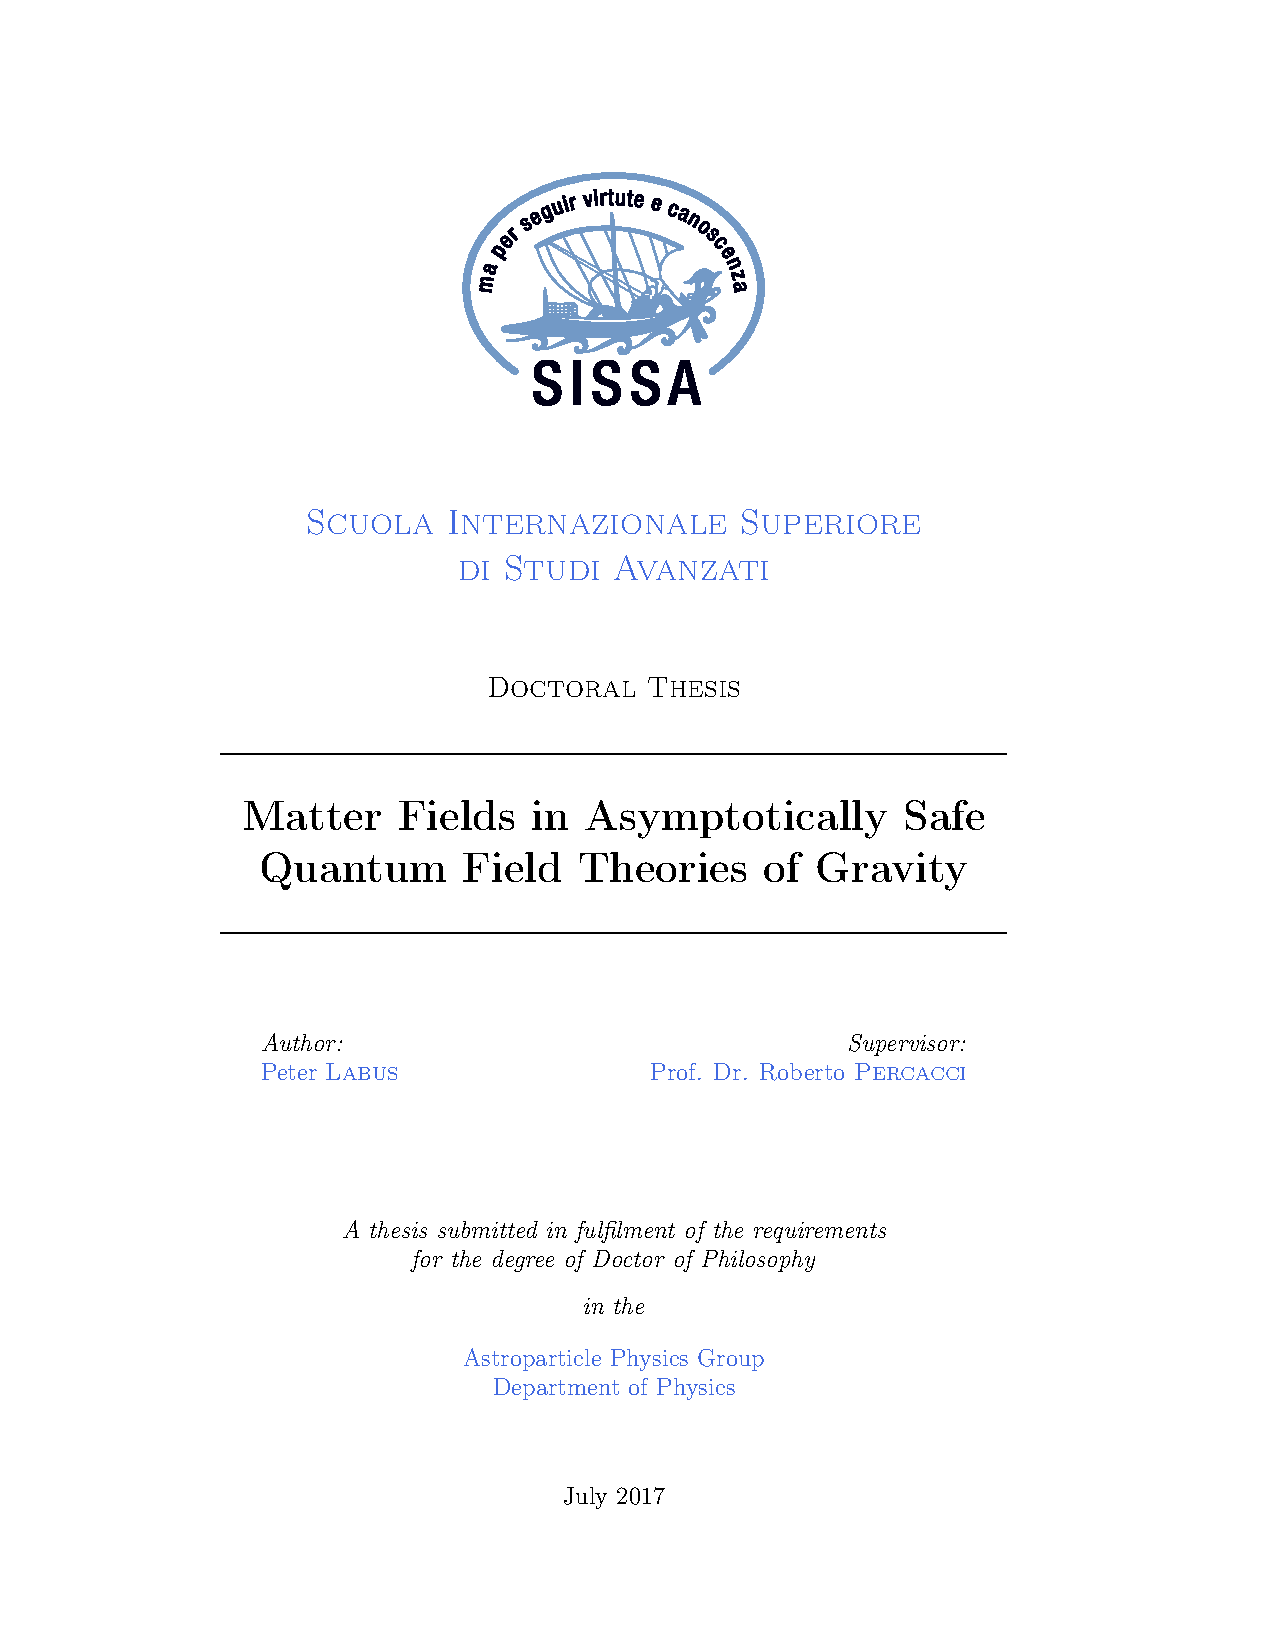
\includepdf{title_page.pdf}

%----------------------------------------------------------------------------------------
% COPYRIGHT PAGE
%----------------------------------------------------------------------------------------

\newpage
~\vfill
\thispagestyle{empty}

\noindent \textsc{PhD Programme in Astroparticle Physics, SISSA Trieste, Italy.}\\

\noindent The research for this PhD thesis project was carried out
under the supervision of Prof.~Dr.~Roberto Percacci with financial support
of a SISSA PhD Fellowship.\\

\noindent \textit{\monthyeardate\today.} % Printing/edition date

%----------------------------------------------------------------------------------------
%	ABSTRACT PAGE
%----------------------------------------------------------------------------------------


% \clearpage
% \phantomsection
\addcontentsline{toc}{chapter}{Abstract}
\chapter*{Abstract}

\vfill
\begin{center}
  Here goes me abstract eventually, \dots
\end{center}
\vfill

%----------------------------------------------------------------------------------------
% ACKNOWLEDGEMENTS
%----------------------------------------------------------------------------------------

\makeatletter
\@openrightfalse
\makeatother

\chapter*{Acknowledgements}
\addcontentsline{toc}{chapter}{Acknowledgements}

It is with great pleasure that I gratefully acknowledge the help and support
% (in no particular order)
of
Roberto~Percacci%
, Tim~R.~Morris%
, Zo\"e~Slade%
, Astrid~Eichhorn%
, Manuel~Reichert%
, Jan~M.~Pawlowski%
, Pietro~Don\`a%
, and
Gian~Paolo~Vacca%
.

\begin{flushright}
  \textit{Peter Labus, \monthyeardate\today.}
\end{flushright}

\makeatletter
\@openrighttrue
\makeatother

%----------------------------------------------------------------------------------------
% TABLE OF CONTENTS
%----------------------------------------------------------------------------------------

\pagestyle{empty} % No headers

\tableofcontents % Print the table of contents itself
% \begingroup
% \let\clearpage\relax
% \listoftables
% \let\clearpage\relax
% \listoffigures
% \endgroup

\pagestyle{fancy} % Print headers again


%----------------------------------------------------------------------------------------
% INTRODUCTION
%----------------------------------------------------------------------------------------

\chapter*{Introduction}
\addcontentsline{toc}{chapter}{\textcolor{ocre}{Introduction}}

\section*{The need for Quantum Gravity}
\addcontentsline{toc}{section}{The need for Quantum Gravity}

% SOURCES:
% https://www.scientificamerican.com/article/physicists-eye-quantum-gravity-interface/
% http://www.einstein-online.info/elementary/quantum/border_regions
% https://www.quora.com/Why-must-there-be-a-quantum-theory-of-gravity
% https://arxiv.org/abs/gr-qc/0606120

The undoubtedly most influential achievements of twentieth century theoretical physics
are the discovery and understanding of
quantum mechanics---including the subsequent construction of quantum field theories---%
as well as the development of general relativity.

The study of quantum field theories in particular has led to the construction
of the standard model of particle physics that describes the three---believed to be---fundamental
strong, weak and electro-magnetic interactions.
Its theory predicts various particles
that have subsequently been discovered by experiments,
such as the W and Z bosons, gluons (via jets), the top and charm quarks, and very recently the Higgs boson.
The sector of strong interactions also predicts confinement of quarks to form hadrons, and
certain observables of the electromagnetic interactions provide the best agreement between
prediction and experiment for any man-made theory (\eg anomalous magnetic dipole moment of the electron).

The general theory of relativity on the other hand, which is a classical theory of gravitation,
has had comparable success and its
classical predictions such as the perihelion precession of Mercury's orbit, the deflection of light by the Sun
and the gravitational redshift of light have long satisfactorily been confirmed by experiments.
More recent experimental/observational tests of the theory include gravitational lensing,
% light travel time delay testing, equivalence principle,
frame-dragging (Lense–Thirring precession),
the cosmological predictions of structure formation
and the recent discovery of gravitational waves.

However, there are still unresolved issues, both what concerns the standard model as well
as general relativity.
The standard model, for instance, suffers from a number of phenomenological issues such as
the precise mechanism to generate the masses of neutrinos,
the structure of dark matter and dark energy,
the mechanism for CP violation needed for early universe baryogenesis,
and the properties of the axion.
Examples of more conceptually related issues include the triviality problem,
the stability of the Higgs potential,
the hierarchy problem,
the cosmological constant problem,
as well as
the origin of the symmetry structure and matter content of the standard model.
% as well as the inclusion of gravitational interactions.

Some of these issues are likely to be resolved by extensions of the standard model
with new matter degrees of freedom, new symmetries and new dynamics. Others, however,
such as the cosmological constant problem or the nature of dark energy,
and even the stability of the Higgs sector
in the ultraviolet (UV) seem to be intricately connected to the gravitational interaction.

But even general relativity by itself clearly reveals boundaries of its applicability.
Most notably, this includes the existence of singularities of physical quantities
in the cases of cosmological and black hole solutions of the theory.
Trying to apply the machinery of quantum mechanics to (ordinary) matter degrees of freedom
whilst keeping the treatment of the gravitational interaction classical has led
to the development of quantum field theory on curved backgrounds. This approach has
been used in the context of early Universe cosmology and cosmological inflation with
great (apparent) success. It however has introduced a great many new questions within
the physics (and in particular thermodynamics) of black holes. This includes the
infamous no-hair theorems, as well as the information paradox.

The general consensus on how to resolve these issues is the quantisation of gravitation
itself---often referred to as quantum gravity.
Apart from the observation that all other known interactions are described by
quantum mechanics, there are usually three arguments brought forward in favour of this
approach.%
\footnote{
  Strictly speaking, all of the following arguments only show that there should be
  a probabilistic theory of gravitation that is compatible with the known
  framework of quantum mechanics used for the other known interactions.
  However, gravity need not be neither quantised nor even a fundamental interaction.
}%
First of all, Einstein's field equations
\begin{align*}
  R_{\mu \nu} - \tfrac{1}{2} \, R \, g_{\mu \nu} = \frac{8 \pi \, \GNewton }{c^4} \, T_{\mu \nu} \,,
\end{align*}
the classical equations of motion of general relativity, couple geometry, \ie the gravitational
field described by the Einstein tensor $G_{\mu\nu} = R_{\mu\nu} - \tfrac{1}{2} \, R \,g_{\mu\nu}$ to
the energy-momentum tensor $T_{\mu\nu}$ of the present matter content. But since ordinary matter
is described by quantum mechanics, the latter is actually a tensor of linear operators rather than
of $c$-numbers. One way to make Einstein's field equations consistent would thus be to
cast the Einstein tensor to an operator as well, \ie quantising the gravitational field.

The second argument, is of similar spirit: Since we know of situations where both gravitational
as well as quantum mechanical phenomena are strong, we need a theory that can consistently
describe both phenomena at the same time. Namely, in black hole thermodynamics,
the Hawking temperature of ordinary matter evaporating from a black hole is given by:
\begin{align*}
  \THawking = \frac{h \, c^3}{\GNewton \, \kBoltzmann} \, \frac {1}{4M} \,.
\end{align*}
Clearly, in natural units quantum mechanical, gravitational, special relativistic and
statistical phenomena are of the same order of magnitude. Since however in quantum mechanics
particles have mass associated with them, and mass couples to gravity, interactions have to
be treated by their full non-linear dynamics given by general relativity,
\ie taking back-reactions of the gravitational
field into account. But since the matter field follows a quantum mechanical probability distribution
the interfering gravitational field must possess a similar probabilistic description as well.

Finally, gravitational waves must necessarily consist of elementary excitations, called gravitons,
otherwise they could be used to determine the path of an electron in a double-slit experiment
without disturbing the interference pattern of the electron field behind the slits. This would
however violate Heisenberg's uncertainty principle.

There have been many approaches towards a theory of quantum gravity
most notably M-theory,
and its low energy limit supergravity,
as well as approaches of canonical quantisation including loop
quantum gravity, its path integral formulation of spin foams and
group field theory. Furthermore, there are theories using an underlying
lattice regularisation such as causal dynamical triangulation and
Regge calculus. There are also approaches emphasising more of the geometrical
nature of general relativity such as causal sets.
All of these formulations are going beyond the framework of quantum
field theories, however, in spite of its successful application within the standard model.

An exception is the so-called asymptotic safety scenario which we want to study
in this thesis. To understand its core idea, let us recall the modern view of
quantum field theories. In contrast to the original understanding that a quantum
field theory has to be (perturbatively) renormalisable in order to be a useful
tool to predict physical quantities, today we regard quantum field theories
as either fundamental or effective, depending on their ultraviolet behaviour.
Namely, any theory without a mathematically well-behaved (\ie finite) ultraviolet
limit, or equivalently one with infinitely many (infrared) relevant directions,
may be called effective. These theories are far from useless, since they allow
to predict \textit{any} physical observable after fixing
only a finite number of parameters
(for instance through a number of independent experiments),
as long as the energy scale is kept below a certain ultraviolet cutoff at the
same time. These effective quantum field theories have been used with great success
in chiral perturbation theory, inflation and even general relativity.%
\footnote{%
  Actually, it is fair to say that the effective field theory of Einstein gravity
  is the best known theory of quantum gravity today. Not only does it combine
  quantum field theory with gravity in a true sense, it also allowed the calculation
  of (at least in principle) falsifiable results, for instance in form of
  corrections to the Newtonian potential.
}
However, they do not allow to extrapolate predictions towards arbitrary energy scales:
this is because of the dependence of observables on infinitely many parameters, which
would require infinitely many, independent experiments to fix them. Fundamental
theories on the other hand only have a finite number of relevant directions which is
to say, they have predictive power at all energy scales after measuring only a
finite number of parameters. Long-known examples of the latter are perturbatively
renormalisable theories without Landau poles---these include the class of Yang-Mills theories,
which have proven to be an excellent tool,
for instance to describe the strong interactions through quantum chromodynamics.
However, since the late 1970s it is known that this scenario is not applicable to
Einstein gravity, and that the latter is not perturbatively renormalisable.

The perturbative renormalisability of Yang-Mills theories may
equally well be viewed as
a collective fixed point of the beta functions of all couplings%
\footnote{%
  Strictly speaking it is enough for all \textit{essential} couplings
  to have a fixed point, that is products and quotients of bare couplings
  that appear in physical observables such as cross sections.
}
of the theory in the ultraviolet. That means that the energy scale dependence
of the couplings becomes self-similar (\ie stable) when approaching arbitrary
high energies. In Yang-Mills theories this is trivially satisfied, because
the essential coupling converges to zero at high energies: quarks and gluons stop interacting
with each other and become free, which is known as asymptotic freedom. The fixed
point in this case is called \textit{free} or \textit{Gaussian}, and it allows
the theory to be studied perturbatively in the ultraviolet. However, the values
of the couplings at the fixed point do not have to be zero for the theory to
be well-behaved in the ultraviolet---it suffices for them to remain finite.
In the latter case the field degrees of freedom will interact with each other at
high energies, which is why the fixed point is called \textit{interacting}.
The general possibility of such a scenario for arbitrary quantum field theory
was first proposed by Steven Weinberg in 1979, \cf Ref.~\cite{Weinberg:1980gg}.
It is since referred to as asymptotic safety following the case of asymptotic
freedom discovered earlier.
The first approach to apply this idea to construct an ultraviolet complete quantum
field theory of gravity was done in 1996 by Martin Reuter, \cf Ref.\cite{Reuter:1996cp}.
Since then, a considerable amount of evidence has been found to support that such
a theory could be constructed for the case of pure gravity.

It is important to mention that the value of the couplings at the fixed point is not
\apriori restricted in any way. In particular, the relevant dimensionless values
may be of order one or greater, forbidding a conventional perturbative study of the theory
at the fixed point by expanding physical observables in powers of the coupling.
This is why the space of all quantum field theories of gravity must be scanned for
candidate theories with non-perturbative tools. Of such there are only a few available,
non of which is as matured as the perturbative tools developed in the last century, yet.
The most notable non-perturbative tools are the conformal bootstrap,
the lattice, entanglement entropy and the functional renormalisation group.
The latter is the traditional tool which has been used in the vast majority
of research concerning asymptotic safety in gravity and it is the one we will use
throughout this thesis as well.


\section*{Outline of the thesis}
\addcontentsline{toc}{section}{Outline of the thesis}

One of the main open issues in asymptotic safety in quantum gravity is
the inclusion of matter field degrees of freedom. Most of this thesis
will deal with this issue in one way or another.

This is interesting and relevant for a number of reason. First of all,
one may argue, that having an ultraviolet complete quantum field theory
of gravity alone is not enough for at least two reasons:
\textit{(a)} the inclusion of matter fields introduces new couplings into
the theory which may behave very differently from the once which couple
gravitons to one another and thus may interfere with asymptotic safety of
pure gravity, or destabilise fixed points entirely;
\textit{(b)} the commonly excepted \textit{effectiveness} of the
standard model has to be dealt with.
In principle it is possible that gravity could cure the instabilities
of the Higgs sector and hence an asymptotically safe quantum
field theory of everything could serve as a nice and elegant ultraviolet completion
of the standard model.

Initial studies of the inclusion of matter fields have indeed revealed that
a large number of scalar fields may destabilise gravitational fixed points
and thus predict an upper bound for the number of scalar matter fields
present in the Universe, \cf Ref.~\cite{Dona:2013qba}. This is especially relevant
for (effective) cosmological theories and (possibly supersymmetric) grand unified
theories which usually incorporate large numbers of scalar fields.
However, there are still many technical details that need to be addressed
in order to solidify these predictions.

A second major reason to study the behaviour of matter fields within a gravitational
quantum field theory concerns the ability to compare predictions of the theory
with experiments and observations. This is in particular true for astrophysical
systems and cosmological test, where couplings between matter and gravity can
be measured much more accurately than observables coming from purely gravitational
effects. This includes the equivalence principle, perturbations of the
cosmic microwave background, implications for inflationary models as well as
even collider experiments.

A second issue we will be (much less) concerned about in this thesis is one of
more technical nature. Namely, we will study some of the implications, the use
of the well-known background field method in quantum field theory has on renormalisation
group properties when defining an energy scale with respect to this very background.%
\footnote{%
  \textit{A priori}, this has nothing to do with diffeomorphism invariance of
  the quantum theory, which is emphasised by other approaches such as loop quantum gravity,
  and may or may not hold at the fixed point in asymptotic safety.
}
This may be regarded as a mathematical consistency condition and could give
interesting insides about the appropriate description of the renormalisation group,
when applied to graviational theories.

\bigskip
\noindent
The thesis is organised as follows:

\medskip
\textbf{Chapter 1} provides a technical introduction to asymptotic safety and the
functional renormalisation group. We will establish most of the mathematical notions
used in later chapters, including truncation schemes, forms of cutoffs and field
parametrisations, as well as basic concepts of critical phenomena. This chapter includes
a detailed case study of a scalar field theory.

\medskip
\textbf{Chapter 2} presents the foundation of the modified split Ward identities and
its application to insure background independence. We study the implications of the
combination of flow equation and Ward identity in the context of conformally reduced
quantum gravity.

\medskip
\textbf{Chapter 3} studies scalar fields non-minimally coupled to a curved background
in a background calculation using heat kernel techniques. We find functional fixed point
solutions and study there linearised behaviour in more details. We discover various
upper bounds for the number of scalar fields when demanding asymptotic safety for
the combined system.

\medskip
\textbf{Chapter 4} augments the previous chapter by studying the dynamics
of a three-leg vertex consisting of two massless scalar fields minimally coupled to
the spin-two mode of a graviton about a flat background.
We find qualitatively similar results as previously and in particular observe
a fixed point destabilising effect induced by the too many scalar fields.

\medskip
\textbf{Chapter 5} repeats the calculation of chapter 4 with different technical choices
such as field parametrisation and cutoff. This shall give an idea about the
robustness of the results obtained so far and the sincerity of the upper bounds.
We also use the Ward identity to remove background dependencies due to the
cutoff operator.


\section*{List of Publications}
\addcontentsline{toc}{section}{List of Publications}

\begin{figure}
  \begin{center}
    \begin{tikzpicture}[
    >=stealth,
    scale=1.00,
  ]

  \tikzmath{
    \rightdistance = -9.8; % right distance for one big table
    % \rightdistance = -4.5; % right distance for one small table
    %                        % and free-standing "main topic"
  }

  % Main table
  \matrix (table) [
    matrix of nodes,
    ]{
    chapter & parametrisation & expansion scheme  & reference \\[2mm]
    Ch. 1   & general         & general    &   \\
    Ch. 2   & any             & derivative &  \cite{Labus:2016lkh} \\
    Ch. 3   & exponential     & derivative &  \cite{Labus:2015ska} \\
    Ch. 4   & exponential     & vertex     &  \cite{Dona:2015tnf} \\
    Ch. 5   & linear          & vertex     &  \cite{Eichhorn:2017aaa} \\
  };

  % Top rule
  \draw[line width=1.5pt] (\rightdistance,  2.00) -- (4.5,  2.00);
  % Mid rule
  \draw[line width=0.55pt](\rightdistance,  1.25) -- (4.5,  1.25);
  % Bottom rule
  \draw[line width=1.5pt] (\rightdistance, -2.00) -- (4.5, -2.00);

  % Main topics on the right
  \node                 at (-7.3,  1.63) {main topic};
  \node[rectangle,draw] at (-7.5,  0.0)  {background independence};
  \node[rectangle,draw] at (-7.4, -1.0)  {scalar matter + gravity};

  % Arrows to "background independence"
  \draw[->] (table-3-1.west) -- (-5.22,  0.00);
  \draw[->] (table-6-1.west) -- (-5.20, -0.05);

  % Arrows to "scalar matter"
  \draw[->] (table-4-1.west) -- (-5.4, -0.9);
  \draw[->] (table-5-1.west) -- (-5.4, -1.0);
  \draw[->] (table-6-1.west) -- (-5.4, -1.1);

\end{tikzpicture}

  \end{center}
  \caption{
    Overview of the chapter contents of the thesis including its main topic, some information
    about technical details used in the calculations and the original reference (where applicable).
  }
  \label{fig:overview}
\end{figure}

The work presented in this thesis is based on the following publications:%
\bigskip
\begin{itemize}
  \setlength\itemsep{0.7em}
  \item \bibentry{Labus:2015ska}
  \item \bibentry{Dona:2015tnf}
  \item \bibentry{Labus:2016lkh}
  \item \bibentry{Eichhorn:2017aaa}
\end{itemize}
\bigskip
An overview, including the main subject of each chapter, technical details
of the respective calculations, as well as the main source of reference, may be found in
Fig.~\ref{fig:overview}.

Most of the diagrams, tables, figures and plots in the original
sources have been recreated for this thesis using \TikZ and \pgfplots, with the exception
of Fig.~\ref{WFN1N2} which was originally created using Wolfram Mathematica~10.0,
and was reproduced here from Ref.~\cite{Labus:2015ska}.
All typesetting has been done with \LaTeX.


%----------------------------------------------------------------------------------------
% CHAPTER 1
%----------------------------------------------------------------------------------------

\mainmatter
\chapter[Asymptotic Safety and the Functional Renormalisation Group]{Asymptotic Safety and the Functional RG}

In this chapter we will explain the idea of asymptotic safety in a
more rigorous way than in the introduction,
and in particular introduced to the notation
used in the rest of this thesis.
To this end, we will first study the functional renormalisation group
equation and its related concepts.
Although the framework of asymptotic safety is quite generic
and could well be studied with other non-perturbative tools, the
language of the renormalisation group turns out to be particularly useful
to explain the core ideas of asymptotic safety.
Our presentation is heavily influenced by
Refs.~\cite{Percacci:2011fr, percacci2017introduction}.

\section{The Wilsonian Renormalisation Group}

In this first section we will introduce the functional renormalisation group as
a tool to solve generic quantum field theories. In particular, we will see how to
formalise Wilson's idea of a coarse-graining procedure for the action
of a quantum field theory by introducing smooth energy scale-dependent
infrared cutoff operators: We will then introduce a scale-dependent
effective average action and derive its exact renormalisation group equation.
Finally, we will discuss some strategies how to obtain approximate solutions
to the exact equation. For reviews of the topics, \cf
\cite{
  Berges:2000ew,
  Aoki:2000wm,
  Pawlowski:2005xe,
  Gies:2006wv,
  Rosten:2010vm
}.


\subsection{Observables in quantum field theories}

In order to solve a quantum field theory, one is interested in
being able to calculate any physical observable the theory may predict.
This will in particular include the existence of particles---elementary
or bound---as well as their properties, such as masses or charges,
but also their behaviour when interacting amongst each other, which
can be quantified using cross-sections.
All of these observables may be expressed using the kinematics
of the theory, as well as its dynamical content, the latter of
which is completely encoded in the so-called $n$-point correlation
functions
\begin{align}
  C_n(x_1, \, x_2,\, \dots, \, x_n) =
  \big\langle  \Phi(x_1) \, \Phi(x_2) \, \dots \, \Phi(x_n) \big\rangle \,,
\end{align}
where the variables $\Phi$ represent (possibly distinct) quantum fields,
which may additionally carry indices of space-time or internal symmetries.
The correlation functions are functional expectation values of products of $n$ field
operators at different space-time positions and they may be
calculated using the path integral formalism via
\begin{align}
  \big\langle  \Phi(x_1) \, \Phi(x_2) \, \dots \, \Phi(x_n) \big\rangle
  = \frac{1}{Z} \int \mathcal D \Phi \;
  \Phi(x_1) \, \Phi(x_2) \, \dots \, \Phi(x_n) \, e^{-S \lbrack \Phi \rbrack } \,,
  \label{eq:expvalue}
\end{align}
where the partition function $Z = \int \mathcal D \Phi \; e^{-S[\Phi]}$ serves as a
normalisation constant, $\mathcal D \Phi$ represents the integration measure,
which iterates over all possible field configurations, and $e^{-S \lbrack \Phi \rbrack}$
is the Euclidean Boltzmann factor---the (quantum) probability distribution
which weights every field configuration in the path integral
according to its classical action.

A more elegant way to obtain any $n$-point correlation function is
by means of the generating functional $W \lbrack J \rbrack$
which is the logarithm of the partition function, to the latter of which
a source term
% $\int \mathrm d^dx \; J(x) \, \Phi(x)$
has been added:%
\footnote{%
  Summation over distinct fields and symmetry indices is explicitly
  understood.
}
\begin{align}
  Z[J] =
  e^{ W \lbrack J \rbrack }
  = \int \mathcal D \Phi \;
  e^{
    - S \lbrack \Phi \rbrack
    + \int \mathrm d^dx \; J(x) \, \Phi(x)
  } \,.
  \label{eq:modpartitionfct}
\end{align}
Taking derivatives with respect to the source term $J$ and evaluating
the expression at $J=0$ yields an efficient procedure to obtain
any correlation function:
\begin{align}
  C_n(x_1, \, x_2,\, \dots, \, x_n) =
  \frac{ \delta W }{ \delta J(x_1) \, \delta J(x_2) \, \dots \, \delta J(x_n) }
  \; \bigg|_{J=0} .
\end{align}
Solving a quantum field theory can
thus equivalently be viewed as calculating the generating functional
(or its image under some one-to-one mapping, such as the
Legendre transformation).
One very common way to do so approximately, is through perturbation
theory. There, one separates the action into a kinetic term, which
describes the freely propagating fields, and a potential term,
which in turn includes the vertices of the theory, \ie the way fields
interact amongst themselves. It is then the latter that is expanded
in powers of some small quantity, such as a coupling parameter,
in order to calculate perturbations around the free theory.
Not only relies this approach on the existence of a small expansion
parameter, it is also by its very nature bound to hide non-analytic
(or non-perturbative) dependencies of observables within the quantum field theory.

An alternative method to calculate the generating functional is based
on Wilson's idea of a functional renormalisation group, and is motivated
by the following observation. With regards to its defining relation,
the generating functional $W$ can be viewed as the quantum equivalent
of the classical (or bare) action $S$.
It is obtained by integrating over all possible quantum mechanical
configurations multiplied with their classical Boltzmann weight.
Furthermore, one can show that the perturbative expansion
(if applicable) of any correlation function
calculated with action $S$ is equivalent to the same expansion
calculated with the `quantum action' $W$, retaining only tree-level
diagrams. This motivates the definition of an energy scale dependent
action $\SLambda$, which is obtained by integrating out
only momentum modes $|q|$ that are higher%
\footnote{%
  In addition we have to regularise the theory in the ultraviolet,
  for instance via a cutoff $\LambdaUV$. However, the details
  of such a procedure are irrelevant for the renormalisation group
  equation discussed here, as will become clear shortly.
}
than some given cutoff scale $\Lambda$
\begin{align}
  e^{ - \SLambda \lbrack \Phi \rbrack }
  = \smashoperator{ \int_{ \Lambda \, \leq \, |q| \, \leq \, \LambdaUV } }
  \mathcal D \Phi \;
  e^{-S \lbrack \Phi \rbrack} \,.
\end{align}
The partition function may then be recovered by integrating out
the remaining modes
\begin{align}
  Z
  = \smashoperator{ \int_{ 0 \, \leq \, |q| \, \leq \, \Lambda } }
  \mathcal D \Phi \;
  e^{-\SLambda \lbrack \Phi \rbrack} \,.
\end{align}
In this way, we can define a scale dependent quantum action which
describes physics at same given energy scale $\Lambda$ in terms of
its tree-level diagrams. In particular, we may quantify the dependence
of $\SLambda$ on the energy scale
through its beta functional $\nicefrac{ \mathrm d\SLambda }{ \mathrm d\Lambda }$,
which can be defined through a first-order integro-differential equation
\begin{align}
  \frac{ \mathrm d \SLambda }{ \mathrm d \Lambda }
  = \lim_{ \delta \Lambda \rightarrow 0 }
  \frac{ S_{\scriptscriptstyle{\Lambda+\delta\Lambda}} - \SLambda }{ \delta \Lambda } \,.
  \label{eq:wilsonRG}
\end{align}
Wilson's renormalisation group thus gives us another strategy to
solve a quantum field theory. In order to do so, we have to find the solution to
the renormalisation group equation with the boundary condition
$S_\LambdaUV = S$,
and subsequently integrate towards the infrared,
$W = - \lim_{\Lambda \rightarrow 0} \SLambda$.

Although this approach does not seem to be any easy than calculating
the original generating functional $W$ directly, it does
offer a number of advantages:
\bigskip
\begin{itemize}
  \setlength\itemsep{1.2mm}
  \item
    The renormalisation group is conceptually simple and physically intuitive.
  \item
    The renormalisation group is non-perturbative.
    In particular, it does not rely on the use of a small expansion parameter.
  \item
    The renormalisation group equation has a simple one-loop form.%
    \footnote{
      This can be seems by rewriting the numerator of the right hand side
      in a perturbative loop expansion. Since the integral is linear
      in its upper and lower boundary, one integrates over a momentum
      shell of thickness $\delta q = \delta \Lambda$,
      such that in each diagram closed loops contribute
      $\nicefrac{\delta \Lambda}{q} \rightarrow 0$, which
      leaves a one-loop contribution only.
    }
  \item
    The resulting beta function is finite.
    In particular, ultraviolet divergences
    that may appear on the right hand side of the renormalisation group
    equation cancel each other.
\end{itemize}
\bigskip
Note that the cutoff $\Lambda$ may be thought of as an ultraviolet cutoff,
since for any given $\SLambda$, it cuts off the high momentum modes in
the path integral, when calculating the partition function.
However, in the definition of $\SLambda$ itself, it is an infrared cutoff
for the high energy modes that get integrated out. For the differential
equation that is the renormalisation group equation, this distinction
clearly does not play any r\^ole. To formalise Wilson's idea and
establish a tool for practical calculations, we will introduce
a smooth infrared cutoff (opposed to the sharp cutoff used before)
and use the Legendre transform of the generating function $W$ to
derive an exact functional renormalisation group equation.


\subsection{Smooth cutoff operators}

Our aim for this subsection is it to introduce a concept of a scale dependent
classical (or bare) action which can then be integrated over in the path
integral to obtain a scale dependent quantum action.

In order to do this, for any given energy scale $k$ we want to distinguish
modes with low momenta $|q|<k$ and modes with high momenta $|q|>k$.
Since it is the high momentum modes we want to integrate out, they should
remain undisturbed by the cutoff procedure, \ie propagate as given by
the theory. The low momentum modes however, should be suppressed, \ie
not be excited and nor propagate. Furthermore, we want to
alter only the propagation of a given mode, and not its interaction structure.
This is why we choose to add to the classical action a cutoff term that is
bilinear in the fields which we want to regulate.

In the most general case of a quantum field theory in curved space-time,
we first have to choose an operator $\mathcal O_\Delta$ which is
a functional of a first or second order differential operator $\Delta$ and
which we leave unspecified for the moment.
Second, we have to calculate the eigenspectrum of the latter
\begin{align}
  \mathcal O_\Delta \, \varphi_n = \lambda_n \, \varphi_n \,.
\end{align}
Then we can expand the quantum field $\varphi(x)$ we want to regularise in terms
of its generalised Fourier coefficients $\phi_n$ as
\begin{align}
  \varphi (x) = \sum_n \; \phi_n \, \varphi_n(x) \,,
\end{align}
where for the moment we assumed a discrete spectrum of $\mathcal O_\Delta$
which we label by integers $n$.
We will outline the case of a scalar field here first,
and comment on how to generalise this procedure to other types of fields
at the end of the subsection. The cutoff term we want to add to the classical
action, can then be written in its most general form in two distinct ways
\begin{align}
  \Delta S_k [\varphi]
  = \frac 12 \int \mathrm d^dx \;
  \varphi(x) \, R_k[ \mathcal O_\Delta ] \, \varphi(x)
  = \frac 12 \sum_n \;
  \phi_n \, R_k(\lambda_n) \, \phi_n \,.
\end{align}
The second expression is often the most convenient form of the cutoff
term when it comes to evaluating functional traces, as the ones that
will appear in the functional renormalisation group equation, see below.
Since it is common practise,
we will denote the cutoff kernel $R_k[ \mathcal O_\Delta ]$
and its Fourier transform with the same symbol, and add its
explicit argument as appropriate.

For a physically more transparent presentation, let us now specialise
to the case of a flat space-time
and $\mathcal O_\Delta = \partial^\mu \partial_\mu$.
The generalised Fourier transformation in this case simply becomes
the usual continuous transformation and the cutoff term in
momentum space assumes the form:%
\footnote{
  Here again we denote Fourier transforms, including the fields themselves,
  with the same symbols as the original variable.
}
\begin{align}
  \Delta S_k [\varphi] = \frac 12 \int \frac{ \mathrm d^dq }{ (2\pi)^d } \;
  \varphi(-q) \, R_k(q^2) \, \varphi(q) \,.
\end{align}
One should think of the regulator $R_k(q^2)$ as a scale-dependent
mass term. To make this idea more precise, let us have a look
at the propagator that results from the introduction of this regulator term:
\begin{align}
  G_k(q^2) = \frac{1}{ q^2 + R_k(q^2) } \,.
\end{align}
It shows clearly, that we indeed introduced an infrared cutoff.
To follow the strategy outlined above, all high momentum modes
should be left unchanged and thus should acquire a mass
$m_k = R_k(q^2) \approx 0$ whenever $|q| > k$. Furthermore,
we may want to make sure that the limit $R_k \rightarrow 0$
happens sufficiently fast (\eg exponentially). The low momentum
modes on the other hand should obtain a mass $m_k = R_k(q^2) \approx k$,
for all $|q| < k$, such that their energy always remains below the mass gap.
It is often beneficent to choose the transition between these two regimes
to be smooth. This is because when dealing with the vertex expansion
approximation scheme of the renormalisation group equation or with
anomalous dimension, their are often times derivatives acting on the cutoff
operator. However, one of the most popular choices of the cutoff operator,
the optimised cutoff, is merely continuous.

\begin{figure}
  \begin{center}
    \begin{tikzpicture}
  \tikzmath{
    \vert = 0.85; % vertical distance between requirements
  }

  \coordinate (base) at (-10.0,  1.5);

  \node[right] (one)   at ($ (base) - (0,0.0*\vert) $) {1. For any $k$ fixed, $R_k(q^2)$ is monotonically decreasing.};
  \node[right] (two)   at ($ (base) - (0,1.0*\vert) $) {2. For any $q^2$ fixed, $R_k(q^2)$ is monotonically increasing.};
  \node[right] (three) at ($ (base) - (0,2.0*\vert) $) {3. For any $q^2 > k^2$, $R_k(q^2) \rightarrow 0$ sufficiently fast.};
  \node[right] (four)  at ($ (base) - (0,3.0*\vert) $) {4. $\lim_{k \rightarrow 0} R_k(q^2) = 0$.};
  \node[right] (five)  at ($ (base) - (0,4.0*\vert) $) {5. $R_k(0) = k^2$.};

  \node[
    draw,
    thick,
    fit={(one) (two) (three) (four) (five)},
    inner sep=8pt
  ] (box) {};

  \begin{groupplot}[
    group style={group size=1 by 2, horizontal sep=10pt, vertical sep=10pt},
    width=3cm,
    height=2.1cm,
    scale only axis,
    major tick length=2pt,
    ]

    \nextgroupplot[ % 1
    xlabel={$q^2$},
    ylabel={$R_{1}(q^2)$},
    xlabel near ticks, xticklabel pos=top,
    xlabel style={at={(0.75,1.08)}},
    ylabel near ticks, yticklabel pos=right,
    xmin=-0.1, xmax=2.1,
    ymin=-0.1, ymax=1.1,
    xtick={0,1.0,2.0},
    ytick={0,0.5,1.0},
    ]
    \addplot[red,thick,domain=0:1,thick]{ 1 - x };
    \addplot[red,thick,domain=1:2,thick]{ 0 };

    \nextgroupplot[ % 2
    xlabel={$k$},
    ylabel={$R_k(1)$},
    xlabel style={at={(0.75,-0.08)}},
    ylabel near ticks, yticklabel pos=right,
    xmin=-0.1, xmax=2.1,
    ymin=-0.1, ymax=1.1,
    xtick={0,1.0,2.0},
    ytick={0,0.5,1.0},
    ]
    \addplot[red,thick,domain=0:1,thick]{ 0 };
    \addplot[red,thick,domain=1:1.42,thick]{ x^2 - 1 };
  \end{groupplot}


\end{tikzpicture}

  \end{center}
  \caption{
    (Left) Formal requirements on a (standard) cutoff operator.
    (Right) Graphical illustration of the first two requirements, using
    the optimised cutoff as an example. The upper panel shows $R_k(q^2)$
    with $k=1$ fixed, and in the lower panel $q^2=1$ is fixed.
    Note that the last three requirements are also satisfied.
  }
  \label{fig:standardcutoff}
\end{figure}

\noindent
We summarise the requirements on the cutoff operator%
\footnote{%
  The requirements listed here characterise a so-called
  standard cutoff. However, we will not be dealing with
  non-standard cutoffs in this thesis.
}
in Fig.~\ref{fig:standardcutoff}. Requirements 1--3
have been explained above%
\footnote{%
  It might be easier to understand requirement 2, by realising
  that for decreasing $k$ the mass gap should reduce for all
  momentum modes $q^2$ simultaneously.
}
and simply implement our cutoff strategy. Requirement 4
is self-evident, as it guarantees to match the standard case when the
cutoff is switched off. The last requirement will turn out to guarantee that
we recover the universal one-loop beta functions for dimensionless
variables. It may be viewed as a normalisation condition.

After this technical motivation, let us now list some examples of
cutoff operators used in actual calculations. Assigning canonical
dimensions to all fields, we can factor out the dimensional
dependence in the cutoff operator and write
\begin{align}
  R_k(q^2) = k^2 \, r(y) \,,
\end{align}
where $y=\nicefrac{q^2}{k^2}$ is the dimensionless momentum
of the modes which get integrated over in the path integral
in units of the squared scale $k^2$, and $r(y)$ is a dimensionless
function, usually called the (cutoff) profile function.
Some popular choices of profile functions include:
\begin{align}
  r(y) &= \frac{ y }{ e^y - 1} \,, \\
  r(y) &= \frac{ y^2 }{ e^{y^2} - 1} \,, \\
  r(y) &= \vphantom{ \frac{ y^2 }{ e^{y^2} - 1} } (1-y) \, \theta(1-y) \,.
\end{align}
The last profile function,
the optimised cutoff, \cf Refs.~\cite{Litim:2000ci,Litim:2001up},
is by far the most widely used.
We display the shapes of these three profiles and the propagator that
result in Fig.~\ref{fig:profiles}.

\begin{figure}
  \begin{center}
    \begin{tikzpicture}
  \begin{groupplot}[
    group style={group size=2 by 1, horizontal sep=10pt, vertical sep=10pt},
    width=0.49\linewidth,
    legend pos=north east,
    legend cell align=left,
    grid=major,
    grid style=dashed,
    ylabel absolute,
    major tick length=2pt,
    ]

    \nextgroupplot[ % 1
    xlabel={momentum $y=\nicefrac{q^2}{k^2}$},
    ylabel={cutoff profile $\; r(y)$},
    xmin=-0.1, xmax=3.1,
    ymin=-0.03, ymax=1.03,
    ytick={0.0,0.25,0.50,0.75,1.0},
    legend style={at={(0.97,0.973)}},
    ]
    \addplot[blue,  thick, domain=0.01:3, samples=100]{ x / ( exp(x) - 1 ) };
    \addplot[green, thick, domain=0.01:3, samples=100]{ x^2 / ( exp(x^2) - 1 ) };
    \addplot[red,   thick, domain=0:1]{ 1 - x };
    \addplot[red,   thick, domain=1:3]{ 0 };
    \legend{
      \, $\frac{ y }{ e^y - 1}$,
      \, $\frac{ y^2 }{ e^{y^2} - 1}$,
      \, $\vphantom{\frac{ y^2 }{ e^{y^2} - 1}} \scriptstyle{(1-y) \, \theta(1-y)}$
    }

    \nextgroupplot[ % 2
    xlabel={momentum $y=\nicefrac{q^2}{k^2}$},
    ylabel near ticks, yticklabel pos=right,
    ylabel={propagator $\; k^2 \, G_k(q^2)$},
    xmin=-0.1, xmax=4.1,
    ymin=-0.05, ymax=2.05,
    legend style={at={(0.978,0.978)},inner sep=5pt},
    ]
    \addplot[black, thick, domain=0.5:4, samples=50, dashed]{ 1/x };
    \addplot[blue,  thick, domain=-0.01:4,   samples=100]{ 1/( x + x / ( exp(x) - 1 ))};
    \addplot[green, thick, domain=-0.01:4,   samples=100]{ 1/( x + x^2 / ( exp(x^2) - 1 ))};
    \addplot[red,   thick, domain=0:1]{ 1 };
    \addplot[red,   thick, domain=1:4]{ 1/x };
    \legend{
      \, $\nicefrac{ 1 }{ y }$,
      \, $\frac{1 - e^{-y}}{y}$,
      \, $\frac{1 - e^{-y^2}}{y^2}$,
      \, $\frac 1{y + (1 - y) \, \theta (1 - y)}$,
    }

  \end{groupplot}
\end{tikzpicture}

  \end{center}
  \caption{
    (Left) Standard profile functions and
    (right) their resulting propagators in units of
    the squared cutoff scale $k^2$.
    The free propagator is added here as reference.
  }
  \label{fig:profiles}
\end{figure}

\noindent
Let us now introduce a cutoff classification that has been
developed in Ref.~\cite{Codello:2008vh}. It is of practical
importance and relies on the observation that the Hessian
of the effective average action, which appears in the
functional renormalisation group equation, as we will see
shortly, is generically proportional to a differential
operator
\begin{align}
  \Delta = - \nabla^2 + \mathbb E \,,
\end{align}
where $\nabla$ is the covariant derivative with respect to
the gauge connection(s), including gravity as well as internal
symmetries, and $\mathbb E$ is a endomorphism which may include
mass terms or curvature invariants. Since the cutoff term will
be added to this Hessian, it will turn out computationally
handy to chose the operator $\mathcal O_\Delta$ of which the cutoff
kernel is a functional to include parts of the operator $\Delta$.
To express the classification, we have to split
the endomorphism $\mathbb E = \mathbb E_1 + \mathbb E_2$
into a part $\mathbb E_1$ which has no scale dependent
couplings and a part $\mathbb E_2$ which contains
renormalisation group dependent couplings only.
Then the following three types of cutoff operators
are defined:
\bigskip
\begin{itemize}
  \setlength\itemsep{2.0mm}
  \item
    {\makebox[2cm]{type I:\hfill}   {$\mathcal O_\Delta = - \nabla^2$}}
  \item
    {\makebox[2cm]{type II:\hfill}  {$\mathcal O_\Delta = - \nabla^2 + \mathbb E_1$}}
  \item
    {\makebox[2cm]{type III:\hfill} {$\mathcal O_\Delta = - \nabla^2 + \mathbb E_1 + \mathbb E_2$}}
\end{itemize}
\bigskip
Note that when using a type III cutoff, the spectrum of the operator
$\mathcal O_\Delta$ will change along the renormalisation group
flow.

To conclude this subsection let us now comment on the case
of having several (possibly multi-component) fields.
The cutoff term is then expressed through a matrix relation
\begin{align}
  \Delta S_k [ \Phi_{\mathcal A} ]
  = \int \mathrm d^dx \;
  \Phi_{\mathcal A} \, R^{\mathcal A \mathcal B}_k \, \Phi_{\mathcal B}
\end{align}
where $\mathcal A$ and $\mathcal B$ iterate over the number
of fields as well as their space-time and possibly internal
indices. Although one could in principle mix different fields
with the same symmetry structure in this way,
$R^{\mathcal A \mathcal B}_k$ is usually chosen to be diagonal
in field space. Also note that this introduces the additional
freedom of choosing the tensor structure of the cutoff.
In practise however, one usually uses the tensor structure
found in the respective Hessian.


\subsection{The effective average action and its exact flow}
\label{sec:floweqn}

Having defined a scale dependent cutoff operator for the
classical action, we can now proceed and define a scale
dependent generating functional via%
\footnote{%
  From now on,
  we will add a tilde above fields which get integrated over in the
  path integral in order to be able to use the same letter for said
  field to denote its classical equivalent, \cf below.
}
\begin{align}
  e^{ W_k \lbrack J \rbrack }
  = \int \mathcal D \tilde \varphi \;
  e^{
    - S \lbrack \tilde \varphi \rbrack
    - \Delta S_k \lbrack \tilde \varphi \rbrack
    + \int \mathrm d^dx \; J(x) \, \tilde \varphi(x)
  } \,.
\end{align}
It will turn out to be more convenient to pass to the
functional Legendre transform of $W_k[J]$,
called the effective average action, which is defined by
\begin{align}
  \hat \Gamma_k [\varphi] = - W_k[J] + \int \mathrm d^dx \; J(x) \, \varphi(x) \,.
\end{align}
Here we have introduced a new variable $\varphi$ as
the functional derivative of the old functional $W_k$ with
respect to the old variable $J$:%
\footnote{%
  Having a finite source function $J(x)$ we can define a
  functional expectation value via
  \begin{align*}
    \big\langle  \mathcal O[\Phi] \big\rangle_J
    \equiv \frac{1}{Z[J]} \int \mathcal D \Phi \;
    \mathcal O[\Phi] \,
    e^{
      - S \lbrack \Phi \rbrack
      + \int \mathrm d^dx \; J(x) \, \Phi(x)
    } \,,
    \label{eq:expvalueJ}
  \end{align*}
  for any field operator $\mathcal O[\Phi]$. This generalises
  Eqn.~\eqref{eq:expvalue} using the modified partition
  function Eqn.~\eqref{eq:modpartitionfct}. Since we do not
  directly want to evaluate partition functions,
  we can always assume $J$ to be non-zero and drop the explicit index.
}
\begin{align}
  \frac{ \delta W_k }{ \delta J(x) }
  = \big\langle \tilde \varphi(x) \big\rangle
  \equiv \varphi (x) \,.
\end{align}
The first equality holds by definition of the generating functional
$W_k$ and the new variable is called the classical field, since
it is exactly this expectation value that appears in the classical
action. The last relation must be invertible such that the old
variable may be expressed in terms of the new one, $J=J[\phi]$.
We can then take the functional derivative of the new function
$\hat \Gamma_k$ with respect to the new variable $\phi$ in order
to discover that
\begin{align}
  \frac{ \delta \hat \Gamma_k }{ \delta \varphi (x) }
  = - \int \mathrm d^dy \; \frac{ \delta W_k }{ \delta J(y) } \,
  \frac{ \delta J(y) }{ \delta \varphi(x) }
  + \int \mathrm d^dy \; \frac{ \delta J(y) }{ \delta \varphi(x) } \, \varphi(x)
  + \int \mathrm d^dy \; J(y) \, \delta(x-y)
  = J(x) \,,
\end{align}
where we made use of the definition of the new variable $\varphi$. Making
use of this observation, we can write the exponential of the negative
effective average action as
\begin{align}
  e^{ - \hat \Gamma_k \lbrack \varphi \rbrack }
  = \int \mathcal D \tilde \varphi \;
  e^{
    - S \lbrack \tilde \varphi \rbrack
    - \Delta S_k \lbrack \tilde \varphi \rbrack
    + \int \mathrm d^dx \;
    \frac{ \delta \hat \Gamma_k }{ \delta \varphi (x) }
    \, \big( \tilde \varphi(x) - \varphi(x) \big)
  } \,.
\end{align}
We can now perform a change of the integration variable
to $\tilde \chi = \tilde \varphi - \varphi$, to obtain
(assuming invariance of the integration measure under
constant shifts):
\begin{align}
  e^{ - \hat \Gamma_k \lbrack \varphi \rbrack }
  = \int \mathcal D \tilde \chi \;
  e^{
    - S \lbrack \tilde \chi + \varphi \rbrack
    - \Delta S_k \lbrack \tilde \chi + \varphi \rbrack
    + \int \mathrm d^dx \;
    \frac{ \delta \hat \Gamma_k }{ \delta \varphi (x) }
    \, \tilde \chi(x)
  } \,.
\end{align}
We will now shift the effective average action by the
cutoff action in order to obtain a more beautiful final
expression:
\begin{align}
  \Gamma_k \equiv \hat \Gamma_k - \Delta S_k \,.
\end{align}
Observing that due to the bilinear form of the cutoff action
we have
\begin{align}
  - \Delta S_k [ \tilde \chi + \varphi ]
  + \Delta S_k [ \varphi ]
  + \int \mathrm d^dx \;
  \frac{ \delta \Delta S_k }{ \delta \varphi (x) }
  \, \tilde \chi(x)
  = - \Delta S_k [ \tilde \chi ] \,,
\end{align}
we finally arrive at the following expression:
\begin{align}
  e^{ - \Gamma_k \lbrack \varphi \rbrack }
  = \int \mathcal D \tilde \chi \;
  e^{
    - S \lbrack \tilde \chi + \varphi \rbrack
    - \Delta S_k \lbrack \tilde \chi \rbrack
    + \int \mathrm d^dx \;
    \frac{ \delta \Gamma_k }{ \delta \varphi (x) }
    \, \tilde \chi(x)
  } \,.
\end{align}
From the last identity, one can show using the
formal requirements on a standard cutoff that
\begin{align}
  \lim_{k \rightarrow 0} \Gamma_k = \Gamma
  \quad \text{and} \quad
  \lim_{k \rightarrow \infty} \Gamma_k = S \,,
\end{align}
where $\Gamma$ is the usual effective action
define without the cutoff action $\Delta S_k$.

We are now ready to derive the exact renormalisation
group equation. To this end we define a renormalisation
group time
\begin{align}
  t \equiv \log \left( \frac k{\mu} \right) ,
\end{align}
where $\mu$ is an arbitrary energy scale. Then from
the definition of the effective average action we
have
\begin{align}
  \frac{ \mathrm d \Gamma_k }{ \mathrm dt }
  = - \frac{ \mathrm d W_k }{ \mathrm dt }
  - \frac{ \mathrm d \Delta S_k }{ \mathrm dt } \,.
\end{align}
The first term can be re-expressed by observing that
\begin{align}
  \frac{ \mathrm d e^{W_k} }{ \mathrm dt }
  = \dot W_k \, e^{W_k}
  = \int \mathcal D \tilde \varphi \;
  \big( - \Delta \dot S_k \big) \,
  e^{
    - S \lbrack \tilde \varphi \rbrack
    - \Delta S_k \lbrack \tilde \varphi \rbrack
    + \int \mathrm d^dx \; J(x) \, \tilde \varphi(x)
  }
  = \big\langle - \Delta \dot S_k \big\rangle \, e^{W_k} \,,
\end{align}
where we used dots to denote derivatives with respect to
time $t$. This expression implies
\begin{align}
  \dot W_k
  = \big\langle - \Delta \dot S_k \big\rangle
  = - \frac 12
  \left\langle
    \int \mathrm d^dx \; \tilde \varphi (x) \, \dot R_k \, \tilde \varphi(x)
  \right\rangle .
\end{align}
Using the fact that the cutoff operator $R_k$ is independent
of the field $\tilde \varphi$ we can write the
% renormalisation group
time derivative of the effective average action as
\begin{align}
  \frac{ \mathrm d \Gamma_k }{ \mathrm dt }
  = \frac 12 \, \Tr
  \left[
    \big(
      \langle \tilde \varphi \tilde \varphi \rangle
      - \langle \tilde \varphi \rangle ^ 2
    \big)
    \, \dot R_k
  \right] ,
\end{align}
where the trace operator $\Tr$ indicates integration
over space-time and momentum, as well as summation over
space-time and internal indices, as appropriate.
To make further progress, we
first note that the definition of $W_k$ implies
\begin{align}
  \frac{ \delta^2 W_k }{ \delta J(x) \, \delta J(y) }
  =
  \big\langle \tilde \varphi (x) \, \tilde \varphi (y) \big\rangle
  - \big\langle \tilde \varphi (x) \big\rangle \big\langle \tilde \varphi (y) \big\rangle \,,
\end{align}
and that we can furthermore re-express the second derivative
acting on $W_k$ as
\begin{align}
  \frac{ \delta^2 W_k }{ \delta J \, \delta J }
  = \frac{ \delta \varphi }{ \delta J }
  = \left( \frac{ \delta J }{ \delta \varphi } \right) ^{\!\! -1}
  = \left( \frac{ \delta^2 \hat \Gamma_k }{ \delta \varphi \, \delta \varphi } \right) ^{\!\! -1} \,.
\end{align}
Here, the first equality follows from the definition of the classical field,
and the last equality from the definition of the Legendre transform.%
\footnote{%
  Note that $W_k$ is a functional of $J$ only.
}
This finally enables us to write
\begin{align}
  \big\langle \tilde \varphi (x) \, \tilde \varphi (x) \big\rangle
  - \big\langle \tilde \varphi (x) \big\rangle \big\langle \tilde \varphi (x) \big\rangle
  = \left( \frac{ \delta^2 \hat \Gamma_k }{ \delta \varphi(x) \, \delta \varphi(x) } \right) ^{\!\! -1} \,.
\end{align}
Substituting the definition of $\Gamma_k$ into the last expression,
we can obtain the exact or functional renormalisation group equation,
also called Wetterich or simply flow equation, as follows
\begin{align}
  % \boxed{
    \frac{ \mathrm d \Gamma_k }{ \mathrm dt }
    = \frac 12 \; \Tr
    \left[
      \left(
        \frac{ \delta^2 \Gamma_k }{ \delta \varphi \, \delta \varphi } + R_k
      \right) ^{\!\!-1}
      \! \dot R_k
    \right] .
  % }
\end{align}
Having formalised Wilson's idea of a functional renormalisation group,
and arrived at a rigorous equivalent to Eqn.~(\ref{eq:wilsonRG}),
some comments are in order. Let us in particular reappraise the
features which we considered advantageous of an renormalisation group approach:
\bigskip
\begin{itemize}
  \setlength\itemsep{1.2mm}
  \item
    \textit{The renormalisation group is conceptually simple and physically intuitive.}
    In particular, it is generic and may be applied to any quantum field theory,
    may it be fundamental or effective.
  \item
    \textit{The renormalisation group is non-perturbative.}
    This is true, since no approximation is made on the way of deriving the
    equation, hence the name ``exact''.
  \item
    \textit{The renormalisation group equation has a simple one-loop form.}
    In particular, it contains a closed loop on its right hand side,
    composed of a full (regularised)  propagator and an insertion
    of the running cutoff operator $\dot R_k$.
    The full propagator, obtained from the quantum effective action contains
    all the non-perturbative information.
    The origin of the one-loop form is manifestly due to the bilinear
    cutoff operator. If one would choose to include higher order terms,
    higher order vertices would appear in the renormalisation group equation.
  \item
    \textit{The resulting beta function is finite.}
    This is due to the fact that $\dot R_k(q^2)$ goes to zero
    sufficiently fast whenever $q^2 > k^2$, thus guaranteeing convergence
    of the momentum integrals in the ultraviolet. The cutoff operator
    $R_k$ additionally imparts an infrared regularisation
    by introducing a mass gap whenever $k \neq 0$.
\end{itemize}
\bigskip
Moreover, given an effective action at some scale $k_0$ the
effective average action can be defined at any other scale $k$
via the function renormalisation group equation. This allows
in particular, as we already anticipated, to calculated the
quantum effective action $\Gamma$ at $k=0$, given that
$\Gamma_k$ has been fixed at some scale $k$ for one reason or another.
Lastly note, that no reference to ultraviolet physics is made
anywhere in the exact renormalisation group equation, \ie
all quantities involved only depend on some intermediate scale $k$.


\subsection{Approximation schemes}
\label{sec:approxschemes}

Now that we have derived an exact renormalisation group equation,
we can discuss strategies how to search for solutions of said equation.
To this end, after having specialised the field content, as well as
all global and/or local (gauge) symmetries, one has to search for solutions
in the space of all quantum field theories with the given properties.
Namely, the effective average action assumes the form
\begin{align}
  \Gamma_k[\Phi] = \sum_{i \in \mathcal I} \; g_i(k) \, \mathcal O_i [\Phi] \,,
  \label{eq:expansionGamma}
\end{align}
which is an infinite sum over a countable index set $\mathcal I$.
Here, the $\mathcal O_i [\Phi]$ represent all monomial operators
which can be build through integration over space-time of powers of
the given fields $\Phi$ and their covariant derivatives, in such a way
that they are scalars under all specified symmetry groups. The coefficients
$g_i(k)$ are hereby scale-dependent coupling constants which in their entirety reflect
the renormalisation group running of the effective average action.
Plugging this expression back into the flow equation yields an equivalent
description in terms of infinitely many coupled equations
in terms of the infinitely many coefficients $g_i(k)$ and their
first derivatives $\dot g_i(k)$ with respect to the renormalisation
group time.

Clearly there is not much hope to find an exact solution to the exact
equation even for the simplest possible choice of field content and
symmetry structure. This is why one has to rely on approximation schemes
to find only approximate solutions to the exact equation. In this
subsection we will introduce the two schemes which are the most relevant for
practical computations and which will be used throughout this thesis.
But before going into the details of these schemes, let us add some
general remarks how to approximate the effective average action in most
cases.

Since we are dealing with a non-perturbative formulation of quantum field
theories, in the most general case there is no (obvious) expansion
parameter available that could reliably be used for the full energy
range from the ultraviolet to the infrared. This is why one often decides
to solve only a finite subset of the infinitely many equation in full theory
space. This approach is called truncation, and effectively shrinks the
index set $\mathcal I$ to some finite, or
infinite, proper subset $\overbar{\mathcal I}$. In the latter case
one usually assumes some functional form for the operators, such as in the
case of $f(R)$ gravity. The choice of the operators involved
in this approximation is arbitrary, but in practise one often chooses
to use the lowest (mass) dimensional operators---as one would do also
in perturbation theory.

Truncations are hard to justify \textit{a priori}, as the renormalisation
group equation couples all operators to every other, at least indirectly.
That is, even setting the running coupling to zero at some scale would
therefore likely imply that it is non-zero at other scales.
Hence a truncation restricts the dynamics possible in the solution quantum
field theory. The common strategy to circumvent this issue is to
subsequently enlarge the truncate space and include higher dimensional operators.
Stability in the behaviour of couplings which were already been included
in previously studied approximations, can than be interpreted as apparent
convergence of the approximate solution. In the framework of asymptotic
safety this procedure can indeed be used to recover well-know
critical behaviour in scalar field theories.

Both of the approximation schemes we want to introduce here make use
of truncations of theory space. The first one, the vertex expansion,
is based on rewriting the sum over all possible operators as a
functional Taylor expansion around some given field configuration
$\bp(x)$:%
\footnote{%
  For simplicity of notation, we will once more return to the
  case of a single scalar field.
}
\begin{align}
  \Gamma_k [\varphi] =
  \sum_{n=0}^{\infty} \; \frac{1}{n!}
  \int \mathrm d^dx_1
  \int \mathrm d^dx_2
  \; \dots \,
  \int \mathrm d^dx_n \;
  \Gamma_{x_1 x_2 \dots x_n}^{(n)} \,
  \prod_{i=1}^n
  \big( \varphi(x_i) - \bp(x_i) \big)
\end{align}
where we introduced the scale-dependent interaction vertices via
\begin{align}
  \Gamma_{x_1 x_2 \dots x_n}^{(n)}[\varphi] \equiv
  \frac{\delta^n\Gamma_k}{\delta\varphi(x_1) \, \delta\varphi(x_2) \, \dots \, \delta\varphi(x_n)} \,,
\end{align}
which are functional derivatives of the full effect average action. These
vertices give their name to the approximation scheme. When plugging the
Taylor expansion back into the renormalisation group equation, we will
obtain a hierarchy of flow equations for each vertex. As we will explicitly
see shortly, these equations are coupled and in particular will the flow of
the $n$-point vertex depend on itself, as well as the $n+1$ and the $n+2$
vertex. That is, to make the scheme useful (and indeed approximate)
we will truncate the resulting system of equations by setting
$\dot \Gamma^{(n)} = 0$ for all $n>\Ntrunc$ and some initial choice of $\Ntrunc$.
Assuming that for any given scale $k$ all vertices $\Gamma^{(n)}$ give
contributions of the same order to the functional traces in the flow equations,
due to the combinatorial factor $\nicefrac{1}{n!}$ in the Taylor expansion,
one might indeed be confident that this approximation scheme is useful.
However, this has to be verified be increasing $\Ntrunc$ iteratively
and investigating the stability of the obtained results.

To explicitly obtain the flow of some $n$-point vertex, one has to take
$n$ functional derivatives of the renormalisation group equation with respect
to the field variable $\varphi(x)$. To do this for the first few vertices
let us introduce a shorthand for the regularised full quantum propagator:
\begin{align}
  \Delta_{xy} [\varphi] \equiv
  \left[
    \frac{\delta^{2}\Gamma_k}{\delta\varphi(x) \, \delta\varphi(y)} + R_k(x,y)
  \right]^{-1} .
\end{align}
Taking one and two functional derivatives, we may than express the running one-
and two-point function in a very compact manner:
\begin{align}
  \partial_t \Gamma^{(1)}_{x} &=
  - \frac 12 \, \Tr
  \left[
    \Delta_{ab} \,
    \Gamma^{(3)}_{bcx} \,
    \Delta_{cd} \,
    \partial_t R_{k,da}
  \right] , \\
  \partial_t \Gamma^{(2)}_{xy} &=
  \Tr
  \left[
    \Delta_{ab} \,
    \Gamma^{(3)}_{bcx} \,
    \Delta_{cd} \,
    \Gamma^{(3)}_{dey} \,
    \Delta_{ef} \,
    \partial_t R_{k,fa}
  \right]
  - \frac 12 \, \Tr
  \left[
    \Delta_{ab} \,
    \Gamma^{(4)}_{bcxy} \,
    \Delta_{cd} \,
    \partial_t R_{k,da}
  \right] .
\end{align}
It is in many ways very instructive to re-express the right hand sides of
these equation in terms of Feynman diagrams. Denoting propagators
as solid lines, the functional traces as closed loops and the regulator
insertion $\partial_t R_k$ with the symbol
\begin{tikzpicture}[
  line width=0.20mm,
  scale=0.5,
  ]

  \tikzmath{
    \radius       = 0.72; % radius of right circle
    \insertradius = 0.20; % radius for regulator insertion
    \degs         = 45;   % angle of insertion X
    \dotradius    = 0.07; % radius of the circles that make the dots
    \leg          = 0.7;  % length external legs
  }

  % Position of the regulator insertion
  \coordinate (X) at (0, \radius);
  \coordinate (A) at (-\radius, 0);
  \coordinate (B) at (0, -\radius);
  \coordinate (C) at (\radius, 0);

  % Regulator insertion \dot R_k
  \fill[white] (X) circle (\insertradius);
  \draw (X) circle (\insertradius);
  \draw (X) -- ($ (X) + ( {cos(\degs)*\insertradius}, {sin(\degs)*\insertradius}) $);
  \draw (X) -- ($ (X) + (-{cos(\degs)*\insertradius}, {sin(\degs)*\insertradius}) $);
  \draw (X) -- ($ (X) + ( {cos(\degs)*\insertradius},-{sin(\degs)*\insertradius}) $);
  \draw (X) -- ($ (X) + (-{cos(\degs)*\insertradius},-{sin(\degs)*\insertradius}) $);

\end{tikzpicture}

\hspace{-2.8mm}
, we can iconographically express the
functional renormalisation group equation as
\begin{align}
  \partial_t \Gamma_k = \frac12 \;
  \begin{tikzpicture}[line width=0.20mm,scale=0.5,baseline=-0.1cm]

  \tikzmath{
    \radius       = 0.72; % radius of right circle
    \insertradius = 0.20; % radius for regulator insertion
    \degs         = 45;   % angle of insertion X
    \dotradius    = 0.07; % radius of the circles that make the dots
  }

  % Position of the regulator insertion
  \coordinate (X) at (0, \radius);

  % Loop composet out of a circle
  \draw  (0, -\radius) arc (-90:270:\radius);

  % Regulator insertion \dot R_k
  \fill[white] (X) circle (\insertradius);
  \draw (X) circle (\insertradius);
  \draw (X) -- ($ (X) + ( {cos(\degs)*\insertradius}, {sin(\degs)*\insertradius}) $);
  \draw (X) -- ($ (X) + (-{cos(\degs)*\insertradius}, {sin(\degs)*\insertradius}) $);
  \draw (X) -- ($ (X) + ( {cos(\degs)*\insertradius},-{sin(\degs)*\insertradius}) $);
  \draw (X) -- ($ (X) + (-{cos(\degs)*\insertradius},-{sin(\degs)*\insertradius}) $);

\end{tikzpicture}
 \;.
\end{align}
Similarly, we can express the running of the first four $n$-point
functions as follows:
\begin{align}
  %%%%%%%%%%%%%%%%%%%%%%%%%%%%%%%%%
  \partial_t \Gamma^{(1)}_{x} &=
  - \, \frac12 \;
  \begin{tikzpicture}[line width=0.20mm,scale=0.5,baseline=-0.1cm]

  \tikzmath{
    \radius       = 0.72; % radius of right circle
    \insertradius = 0.20; % radius for regulator insertion
    \degs         = 45;   % angle of insertion X
    \dotradius    = 0.07; % radius of the circles that make the dots
    \leg          = 0.7;  % length external legs
  }

  % Position of the regulator insertion
  \coordinate (X) at (0, \radius);
  \coordinate (A) at (-\radius, 0);
  \coordinate (B) at (0, -\radius);
  \coordinate (C) at (\radius, 0);

  % Loop composet out of a circle
  \draw  (0, -\radius) arc (-90:270:\radius);

  % Regulator insertion \dot R_k
  \fill[white] (X) circle (\insertradius);
  \draw (X) circle (\insertradius);
  \draw (X) -- ($ (X) + ( {cos(\degs)*\insertradius}, {sin(\degs)*\insertradius}) $);
  \draw (X) -- ($ (X) + (-{cos(\degs)*\insertradius}, {sin(\degs)*\insertradius}) $);
  \draw (X) -- ($ (X) + ( {cos(\degs)*\insertradius},-{sin(\degs)*\insertradius}) $);
  \draw (X) -- ($ (X) + (-{cos(\degs)*\insertradius},-{sin(\degs)*\insertradius}) $);

  % external leg
  \draw[fill] (B) circle [radius=\dotradius];
  \draw (B) -- ($ (B) + (0, -\leg) $)
  node[right, inner sep=0.7mm] {$\scriptstyle x$};

\end{tikzpicture}
 \;,
  \label{eq:deriv1} \\
  %%%%%%%%%%%%%%%%%%%%%%%%%%%%%%%%%
  \partial_t \Gamma^{(2)}_{xy} &=
  \, \begin{tikzpicture}[line width=0.20mm,scale=0.5,baseline=-0.1cm]

  \tikzmath{
    \radius       = 0.72; % radius of right circle
    \insertradius = 0.20; % radius for regulator insertion
    \degs         = 45;   % angle of insertion X
    \dotradius    = 0.07; % radius of the circles that make the dots
    \leg          = 0.7;  % length external legs
  }

  % Position of the regulator insertion
  \coordinate (X) at (0, \radius);
  \coordinate (A) at (-\radius, 0);
  \coordinate (B) at (0, -\radius);
  \coordinate (C) at (\radius, 0);

  % Loop composet out of a circle
  \draw  (0, -\radius) arc (-90:270:\radius);

  % Regulator insertion \dot R_k
  \fill[white] (X) circle (\insertradius);
  \draw (X) circle (\insertradius);
  \draw (X) -- ($ (X) + ( {cos(\degs)*\insertradius}, {sin(\degs)*\insertradius}) $);
  \draw (X) -- ($ (X) + (-{cos(\degs)*\insertradius}, {sin(\degs)*\insertradius}) $);
  \draw (X) -- ($ (X) + ( {cos(\degs)*\insertradius},-{sin(\degs)*\insertradius}) $);
  \draw (X) -- ($ (X) + (-{cos(\degs)*\insertradius},-{sin(\degs)*\insertradius}) $);

  % external legs
  \draw[fill] (A) circle [radius=\dotradius];
  \draw (A) -- ($ (A) + (-\leg, 0) $)
  node[below, inner sep=0.7mm] {$\scriptstyle x$};
  \draw[fill] (C) circle [radius=\dotradius];
  \draw (C) -- ($ (C) + ( \leg, 0) $)
  node[below, inner sep=0.7mm] {$\scriptstyle y$};

\end{tikzpicture}

  - \frac12 \;
  \begin{tikzpicture}[line width=0.20mm,scale=0.5,baseline=-0.1cm]

  \tikzmath{
    \radius       = 0.72; % radius of right circle
    \insertradius = 0.20; % radius for regulator insertion
    \degs         = 45;   % angle of insertion X
    \dotradius    = 0.07; % radius of the circles that make the dots
    \leg          = 0.7;  % length external legs
  }

  % Position of the regulator insertion
  \coordinate (X) at (0, \radius);
  \coordinate (A) at (-\radius, 0);
  \coordinate (B) at (0, -\radius);
  \coordinate (C) at (\radius, 0);

  % Loop composet out of a circle
  \draw  (0, -\radius) arc (-90:270:\radius);

  % Regulator insertion \dot R_k
  \fill[white] (X) circle (\insertradius);
  \draw (X) circle (\insertradius);
  \draw (X) -- ($ (X) + ( {cos(\degs)*\insertradius}, {sin(\degs)*\insertradius}) $);
  \draw (X) -- ($ (X) + (-{cos(\degs)*\insertradius}, {sin(\degs)*\insertradius}) $);
  \draw (X) -- ($ (X) + ( {cos(\degs)*\insertradius},-{sin(\degs)*\insertradius}) $);
  \draw (X) -- ($ (X) + (-{cos(\degs)*\insertradius},-{sin(\degs)*\insertradius}) $);

  % external legs
  \draw[fill] (B) circle [radius=\dotradius];
  \draw (B) -- ($ (B) + (-{cos(\degs)*\leg},-{sin(\degs)*\leg}) $)
  node[below, inner sep=0.6mm] {$\scriptstyle x$};
  \draw (B) -- ($ (B) + ( {cos(\degs)*\leg},-{sin(\degs)*\leg}) $)
  node[below, inner sep=0.6mm] {$\scriptstyle y$};

\end{tikzpicture}
 \;,
  \label{eq:deriv2} \\
  %%%%%%%%%%%%%%%%%%%%%%%%%%%%%%%%%
  \partial_t \Gamma^{(3)}_{xyz} &=
  - \, 3 \;
  \begin{tikzpicture}[line width=0.20mm,scale=0.5,baseline=-0.1cm]

  \tikzmath{
    \radius       = 0.72; % radius of right circle
    \insertradius = 0.20; % radius for regulator insertion
    \degs         = 45;   % angle of insertion X
    \dotradius    = 0.07; % radius of the circles that make the dots
    \leg          = 0.7;  % length external legs
  }

  % Position of the regulator insertion
  \coordinate (X) at (0, \radius);
  \coordinate (A) at (-\radius, 0);
  \coordinate (B) at (0, -\radius);
  \coordinate (C) at (\radius, 0);

  % Loop composet out of a circle
  \draw  (0, -\radius) arc (-90:270:\radius);

  % Regulator insertion \dot R_k
  \fill[white] (X) circle (\insertradius);
  \draw (X) circle (\insertradius);
  \draw (X) -- ($ (X) + ( {cos(\degs)*\insertradius}, {sin(\degs)*\insertradius}) $);
  \draw (X) -- ($ (X) + (-{cos(\degs)*\insertradius}, {sin(\degs)*\insertradius}) $);
  \draw (X) -- ($ (X) + ( {cos(\degs)*\insertradius},-{sin(\degs)*\insertradius}) $);
  \draw (X) -- ($ (X) + (-{cos(\degs)*\insertradius},-{sin(\degs)*\insertradius}) $);

  % external legs
  \draw[fill] (A) circle [radius=\dotradius];
  \draw (A) -- ($ (A) + (-\leg, 0) $)
  node[below, inner sep=0.7mm] {$\scriptstyle x$};

  \draw[fill] (B) circle [radius=\dotradius];
  \draw (B) -- ($ (B) + ( 0, -\leg) $)
  node[right, inner sep=0.7mm] {$\scriptstyle y$};

  \draw[fill] (C) circle [radius=\dotradius];
  \draw (C) -- ($ (C) + ( \leg, 0) $)
  node[below, inner sep=0.7mm] {$\scriptstyle z$};

\end{tikzpicture}

  - \frac12 \;
  \begin{tikzpicture}[line width=0.20mm,scale=0.5,baseline=-0.1cm]

  \tikzmath{
    \radius       = 0.72; % radius of right circle
    \insertradius = 0.20; % radius for regulator insertion
    \degs         = 45;   % angle of insertion X
    \dotradius    = 0.07; % radius of the circles that make the dots
    \leg          = 0.7;  % length external legs
  }

  % Position of the regulator insertion
  \coordinate (X) at (0, \radius);
  \coordinate (A) at (-\radius, 0);
  \coordinate (B) at (0, -\radius);
  \coordinate (C) at (\radius, 0);

  % Loop composet out of a circle
  \draw  (0, -\radius) arc (-90:270:\radius);

  % Regulator insertion \dot R_k
  \fill[white] (X) circle (\insertradius);
  \draw (X) circle (\insertradius);
  \draw (X) -- ($ (X) + ( {cos(\degs)*\insertradius}, {sin(\degs)*\insertradius}) $);
  \draw (X) -- ($ (X) + (-{cos(\degs)*\insertradius}, {sin(\degs)*\insertradius}) $);
  \draw (X) -- ($ (X) + ( {cos(\degs)*\insertradius},-{sin(\degs)*\insertradius}) $);
  \draw (X) -- ($ (X) + (-{cos(\degs)*\insertradius},-{sin(\degs)*\insertradius}) $);

  % external legs
  \draw[fill] (B) circle [radius=\dotradius];

  \draw (B) -- ($ (B) + (-{cos(\degs)*\leg},-{sin(\degs)*\leg}) $)
  node[below, inner sep=0.6mm] {$\scriptstyle x$};

  \draw (B) -- ($ (B) + ( 0, -\leg) $)
  node[below, inner sep=0.7mm] {$\scriptstyle y$};

  \draw (B) -- ($ (B) + ( {cos(\degs)*\leg},-{sin(\degs)*\leg}) $)
  node[below, inner sep=0.6mm] {$\scriptstyle z$};

\end{tikzpicture}

  + \begin{tikzpicture}[line width=0.20mm,scale=0.5,baseline=-0.1cm]

  \tikzmath{
    \radius       = 0.72; % radius of right circle
    \insertradius = 0.20; % radius for regulator insertion
    \degs         = 45;   % angle of insertion X
    \dotradius    = 0.07; % radius of the circles that make the dots
    \leg          = 0.7;  % length external legs
  }

  % Position of the regulator insertion
  \coordinate (X) at (0, \radius);
  \coordinate (A) at (-\radius, 0);
  \coordinate (B) at (0, -\radius);
  \coordinate (C) at (\radius, 0);

  % Loop composet out of a circle
  \draw  (0, -\radius) arc (-90:270:\radius);

  % Regulator insertion \dot R_k
  \fill[white] (X) circle (\insertradius);
  \draw (X) circle (\insertradius);
  \draw (X) -- ($ (X) + ( {cos(\degs)*\insertradius}, {sin(\degs)*\insertradius}) $);
  \draw (X) -- ($ (X) + (-{cos(\degs)*\insertradius}, {sin(\degs)*\insertradius}) $);
  \draw (X) -- ($ (X) + ( {cos(\degs)*\insertradius},-{sin(\degs)*\insertradius}) $);
  \draw (X) -- ($ (X) + (-{cos(\degs)*\insertradius},-{sin(\degs)*\insertradius}) $);

  % external legs
  \draw[fill] (A) circle [radius=\dotradius];
  \draw (A) -- ($ (A) + (-\leg, 0) $)
  node[below, inner sep=0.7mm] {$\scriptstyle x$};

  \draw[fill] (C) circle [radius=\dotradius];
  \draw (C) -- ($ (C) + ({cos(\degs)*\leg}, {sin(\degs)*\leg}) $)
  node[above, inner sep=0.7mm] {$\scriptstyle y$};

  \draw (C) -- ($ (C) + ({cos(\degs)*\leg},-{sin(\degs)*\leg}) $)
  node[below, inner sep=0.7mm] {$\scriptstyle z$};

\end{tikzpicture}

  + \begin{tikzpicture}[line width=0.20mm,scale=0.5,baseline=-0.1cm]

  \tikzmath{
    \radius       = 0.72; % radius of right circle
    \insertradius = 0.20; % radius for regulator insertion
    \degs         = 45;   % angle of insertion X
    \dotradius    = 0.07; % radius of the circles that make the dots
    \leg          = 0.7;  % length external legs
  }

  % Position of the regulator insertion
  \coordinate (X) at (0, \radius);
  \coordinate (A) at (-\radius, 0);
  \coordinate (B) at (0, -\radius);
  \coordinate (C) at (\radius, 0);

  % Loop composet out of a circle
  \draw  (0, -\radius) arc (-90:270:\radius);

  % Regulator insertion \dot R_k
  \fill[white] (X) circle (\insertradius);
  \draw (X) circle (\insertradius);
  \draw (X) -- ($ (X) + ( {cos(\degs)*\insertradius}, {sin(\degs)*\insertradius}) $);
  \draw (X) -- ($ (X) + (-{cos(\degs)*\insertradius}, {sin(\degs)*\insertradius}) $);
  \draw (X) -- ($ (X) + ( {cos(\degs)*\insertradius},-{sin(\degs)*\insertradius}) $);
  \draw (X) -- ($ (X) + (-{cos(\degs)*\insertradius},-{sin(\degs)*\insertradius}) $);

  % external legs
  \draw[fill] (A) circle [radius=\dotradius];
  \draw (A) -- ($ (A) + (-\leg, 0) $)
  node[below, inner sep=0.7mm] {$\scriptstyle y$};

  \draw[fill] (C) circle [radius=\dotradius];
  \draw (C) -- ($ (C) + ({cos(\degs)*\leg}, {sin(\degs)*\leg}) $)
  node[above, inner sep=0.7mm] {$\scriptstyle x$};

  \draw (C) -- ($ (C) + ({cos(\degs)*\leg},-{sin(\degs)*\leg}) $)
  node[below, inner sep=0.7mm] {$\scriptstyle z$};

\end{tikzpicture}

  + \begin{tikzpicture}[line width=0.20mm,scale=0.5,baseline=-0.1cm]

  \tikzmath{
    \radius       = 0.72; % radius of right circle
    \insertradius = 0.20; % radius for regulator insertion
    \degs         = 45;   % angle of insertion X
    \dotradius    = 0.07; % radius of the circles that make the dots
    \leg          = 0.7;  % length external legs
  }

  % Position of the regulator insertion
  \coordinate (X) at (0, \radius);
  \coordinate (A) at (-\radius, 0);
  \coordinate (B) at (0, -\radius);
  \coordinate (C) at (\radius, 0);

  % Loop composet out of a circle
  \draw  (0, -\radius) arc (-90:270:\radius);

  % Regulator insertion \dot R_k
  \fill[white] (X) circle (\insertradius);
  \draw (X) circle (\insertradius);
  \draw (X) -- ($ (X) + ( {cos(\degs)*\insertradius}, {sin(\degs)*\insertradius}) $);
  \draw (X) -- ($ (X) + (-{cos(\degs)*\insertradius}, {sin(\degs)*\insertradius}) $);
  \draw (X) -- ($ (X) + ( {cos(\degs)*\insertradius},-{sin(\degs)*\insertradius}) $);
  \draw (X) -- ($ (X) + (-{cos(\degs)*\insertradius},-{sin(\degs)*\insertradius}) $);

  % external legs
  \draw[fill] (A) circle [radius=\dotradius];
  \draw (A) -- ($ (A) + (-\leg, 0) $)
  node[below, inner sep=0.7mm] {$\scriptstyle z$};

  \draw[fill] (C) circle [radius=\dotradius];
  \draw (C) -- ($ (C) + ({cos(\degs)*\leg}, {sin(\degs)*\leg}) $)
  node[above, inner sep=0.7mm] {$\scriptstyle x$};

  \draw (C) -- ($ (C) + ({cos(\degs)*\leg},-{sin(\degs)*\leg}) $)
  node[below, inner sep=0.7mm] {$\scriptstyle y$};

\end{tikzpicture}

  \;,
  \label{eq:deriv3} \\
  %%%%%%%%%%%%%%%%%%%%%%%%%%%%%%%%%
  \partial_t \Gamma^{(4)}_{xyzw} &=
  \, 3 \; \begin{tikzpicture}[line width=0.20mm,scale=0.5,baseline=-0.1cm]

  \tikzmath{
    \radius       = 0.72; % radius of right circle
    \insertradius = 0.20; % radius for regulator insertion
    \degs         = 45;   % angle of insertion X
    \degsleg      = 35;   % angle in circle for external leg
    \dotradius    = 0.07; % radius of the circles that make the dots
    \leg          = 0.7;  % length external legs
  }

  % Position of the regulator insertion
  \coordinate (X) at (0, \radius);
  \coordinate (A) at (-{cos(\degsleg)*\radius},  {sin(\degsleg)*\radius});
  \coordinate (B) at (-{cos(\degsleg)*\radius}, -{sin(\degsleg)*\radius});
  \coordinate (C) at ( {cos(\degsleg)*\radius}, -{sin(\degsleg)*\radius});
  \coordinate (D) at ( {cos(\degsleg)*\radius},  {sin(\degsleg)*\radius});

  % Loop composet out of a circle
  \draw  (0, -\radius) arc (-90:270:\radius);

  % Regulator insertion \dot R_k
  \fill[white] (X) circle (\insertradius);
  \draw (X) circle (\insertradius);
  \draw (X) -- ($ (X) + ( {cos(\degs)*\insertradius}, {sin(\degs)*\insertradius}) $);
  \draw (X) -- ($ (X) + (-{cos(\degs)*\insertradius}, {sin(\degs)*\insertradius}) $);
  \draw (X) -- ($ (X) + ( {cos(\degs)*\insertradius},-{sin(\degs)*\insertradius}) $);
  \draw (X) -- ($ (X) + (-{cos(\degs)*\insertradius},-{sin(\degs)*\insertradius}) $);

  % external legs
  \draw[fill] (A) circle [radius=\dotradius];
  \draw (A) -- ($ (A) + (-{cos(\degs)*\leg}, {sin(\degs)*\leg}) $)
  node[left, inner sep=0.5mm] {$\scriptstyle x$};

  \draw[fill] (B) circle [radius=\dotradius];
  \draw (B) -- ($ (B) + (-{cos(\degs)*\leg}, -{sin(\degs)*\leg}) $)
  node[left, inner sep=0.5mm] {$\scriptstyle y$};

  \draw[fill] (C) circle [radius=\dotradius];
  \draw (C) -- ($ (C) + ( {cos(\degs)*\leg}, -{sin(\degs)*\leg}) $)
  node[right, inner sep=0.5mm] {$\scriptstyle z$};

  \draw[fill] (D) circle [radius=\dotradius];
  \draw (D) -- ($ (D) + ( {cos(\degs)*\leg},  {sin(\degs)*\leg}) $)
  node[right, inner sep=0.5mm] {$\scriptstyle w$};

\end{tikzpicture}

  - \frac12 \; \begin{tikzpicture}[line width=0.20mm,scale=0.5,baseline=-0.1cm]

  \tikzmath{
    \radius       = 0.72; % radius of right circle
    \insertradius = 0.20; % radius for regulator insertion
    \degs         = 45;   % angle of insertion X
    \degstwo      = 55;   % angle of external legs
    \dotradius    = 0.07; % radius of the circles that make the dots
    \leg          = 0.7;  % length external legs
  }

  % Position of the regulator insertion
  \coordinate (X) at (0, \radius);
  \coordinate (A) at (-\radius, 0);
  \coordinate (B) at (0, -\radius);
  \coordinate (C) at (\radius, 0);

  % Loop composet out of a circle
  \draw  (0, -\radius) arc (-90:270:\radius);

  % Regulator insertion \dot R_k
  \fill[white] (X) circle (\insertradius);
  \draw (X) circle (\insertradius);
  \draw (X) -- ($ (X) + ( {cos(\degs)*\insertradius}, {sin(\degs)*\insertradius}) $);
  \draw (X) -- ($ (X) + (-{cos(\degs)*\insertradius}, {sin(\degs)*\insertradius}) $);
  \draw (X) -- ($ (X) + ( {cos(\degs)*\insertradius},-{sin(\degs)*\insertradius}) $);
  \draw (X) -- ($ (X) + (-{cos(\degs)*\insertradius},-{sin(\degs)*\insertradius}) $);

  % external legs
  \draw[fill] (B) circle [radius=\dotradius];

  \draw (B) -- ($ (B) + (-\leg, 0) $)
  node[below, inner sep=0.7mm] {$\scriptstyle x$};

  \draw (B) -- ($ (B) + (-{cos(\degstwo)*\leg},-{sin(\degstwo)*\leg}) $)
  node[below, inner sep=0.6mm] {$\scriptstyle y$};

  \draw (B) -- ($ (B) + ( {cos(\degstwo)*\leg},-{sin(\degstwo)*\leg}) $)
  node[below, inner sep=0.6mm] {$\scriptstyle z$};

  \draw (B) -- ($ (B) + ( \leg, 0) $)
  node[below, inner sep=0.7mm] {$\scriptstyle w$};

\end{tikzpicture}

  - \begin{tikzpicture}[line width=0.20mm,scale=0.5,baseline=-0.1cm]

  \tikzmath{
    \radius       = 0.72; % radius of right circle
    \insertradius = 0.20; % radius for regulator insertion
    \degs         = 45;   % angle of insertion X
    \degsleg      = 30;   % angle in circle for external leg
    \dotradius    = 0.07; % radius of the circles that make the dots
    \leg          = 0.7;  % length external legs
  }

  % Position of the regulator insertion
  \coordinate (X) at (0, \radius);
  \coordinate (A) at (-{cos(\degsleg)*\radius}, {sin(\degsleg)*\radius});
  \coordinate (D) at (-{cos(\degsleg)*\radius}, -{sin(\degsleg)*\radius});
  \coordinate (B) at (0, -\radius);
  \coordinate (C) at (\radius, 0);

  % Loop composet out of a circle
  \draw  (0, -\radius) arc (-90:270:\radius);

  % Regulator insertion \dot R_k
  \fill[white] (X) circle (\insertradius);
  \draw (X) circle (\insertradius);
  \draw (X) -- ($ (X) + ( {cos(\degs)*\insertradius}, {sin(\degs)*\insertradius}) $);
  \draw (X) -- ($ (X) + (-{cos(\degs)*\insertradius}, {sin(\degs)*\insertradius}) $);
  \draw (X) -- ($ (X) + ( {cos(\degs)*\insertradius},-{sin(\degs)*\insertradius}) $);
  \draw (X) -- ($ (X) + (-{cos(\degs)*\insertradius},-{sin(\degs)*\insertradius}) $);

  % external legs
  \draw[fill] (A) circle [radius=\dotradius];
  \draw (A) -- ($ (A) + (-\leg, 0) $)
  node[above, inner sep=0.7mm] {$\scriptstyle x$};

  \draw[fill] (D) circle [radius=\dotradius];
  \draw (D) -- ($ (D) + (-\leg, 0) $)
  node[below, inner sep=0.7mm] {$\scriptstyle y$};

  \draw[fill] (C) circle [radius=\dotradius];
  \draw (C) -- ($ (C) + ({cos(\degs)*\leg}, {sin(\degs)*\leg}) $)
  node[above, inner sep=0.7mm] {$\scriptstyle z$};

  \draw (C) -- ($ (C) + ({cos(\degs)*\leg},-{sin(\degs)*\leg}) $)
  node[below, inner sep=0.7mm] {$\scriptstyle w$};

\end{tikzpicture}

  - \begin{tikzpicture}[line width=0.20mm,scale=0.5,baseline=-0.1cm]

  \tikzmath{
    \radius       = 0.72; % radius of right circle
    \insertradius = 0.20; % radius for regulator insertion
    \degs         = 45;   % angle of insertion X
    \degsleg      = 30;   % angle in circle for external leg
    \dotradius    = 0.07; % radius of the circles that make the dots
    \leg          = 0.7;  % length external legs
  }

  % Position of the regulator insertion
  \coordinate (X) at (0, \radius);
  \coordinate (A) at (-{cos(\degsleg)*\radius}, {sin(\degsleg)*\radius});
  \coordinate (D) at (-{cos(\degsleg)*\radius}, -{sin(\degsleg)*\radius});
  \coordinate (B) at (0, -\radius);
  \coordinate (C) at (\radius, 0);

  % Loop composet out of a circle
  \draw  (0, -\radius) arc (-90:270:\radius);

  % Regulator insertion \dot R_k
  \fill[white] (X) circle (\insertradius);
  \draw (X) circle (\insertradius);
  \draw (X) -- ($ (X) + ( {cos(\degs)*\insertradius}, {sin(\degs)*\insertradius}) $);
  \draw (X) -- ($ (X) + (-{cos(\degs)*\insertradius}, {sin(\degs)*\insertradius}) $);
  \draw (X) -- ($ (X) + ( {cos(\degs)*\insertradius},-{sin(\degs)*\insertradius}) $);
  \draw (X) -- ($ (X) + (-{cos(\degs)*\insertradius},-{sin(\degs)*\insertradius}) $);

  % external legs
  \draw[fill] (A) circle [radius=\dotradius];
  \draw (A) -- ($ (A) + (-\leg, 0) $)
  node[above, inner sep=0.7mm] {$\scriptstyle x$};

  \draw[fill] (D) circle [radius=\dotradius];
  \draw (D) -- ($ (D) + (-\leg, 0) $)
  node[below, inner sep=0.7mm] {$\scriptstyle z$};

  \draw[fill] (C) circle [radius=\dotradius];
  \draw (C) -- ($ (C) + ({cos(\degs)*\leg}, {sin(\degs)*\leg}) $)
  node[above, inner sep=0.7mm] {$\scriptstyle y$};

  \draw (C) -- ($ (C) + ({cos(\degs)*\leg},-{sin(\degs)*\leg}) $)
  node[below, inner sep=0.7mm] {$\scriptstyle w$};

\end{tikzpicture}

  - \begin{tikzpicture}[line width=0.20mm,scale=0.5,baseline=-0.1cm]

  \tikzmath{
    \radius       = 0.72; % radius of right circle
    \insertradius = 0.20; % radius for regulator insertion
    \degs         = 45;   % angle of insertion X
    \degsleg      = 30;   % angle in circle for external leg
    \dotradius    = 0.07; % radius of the circles that make the dots
    \leg          = 0.7;  % length external legs
  }

  % Position of the regulator insertion
  \coordinate (X) at (0, \radius);
  \coordinate (A) at (-{cos(\degsleg)*\radius}, {sin(\degsleg)*\radius});
  \coordinate (D) at (-{cos(\degsleg)*\radius}, -{sin(\degsleg)*\radius});
  \coordinate (B) at (0, -\radius);
  \coordinate (C) at (\radius, 0);

  % Loop composet out of a circle
  \draw  (0, -\radius) arc (-90:270:\radius);

  % Regulator insertion \dot R_k
  \fill[white] (X) circle (\insertradius);
  \draw (X) circle (\insertradius);
  \draw (X) -- ($ (X) + ( {cos(\degs)*\insertradius}, {sin(\degs)*\insertradius}) $);
  \draw (X) -- ($ (X) + (-{cos(\degs)*\insertradius}, {sin(\degs)*\insertradius}) $);
  \draw (X) -- ($ (X) + ( {cos(\degs)*\insertradius},-{sin(\degs)*\insertradius}) $);
  \draw (X) -- ($ (X) + (-{cos(\degs)*\insertradius},-{sin(\degs)*\insertradius}) $);

  % external legs
  \draw[fill] (A) circle [radius=\dotradius];
  \draw (A) -- ($ (A) + (-\leg, 0) $)
  node[above, inner sep=0.7mm] {$\scriptstyle x$};

  \draw[fill] (D) circle [radius=\dotradius];
  \draw (D) -- ($ (D) + (-\leg, 0) $)
  node[below, inner sep=0.7mm] {$\scriptstyle w$};

  \draw[fill] (C) circle [radius=\dotradius];
  \draw (C) -- ($ (C) + ({cos(\degs)*\leg}, {sin(\degs)*\leg}) $)
  node[above, inner sep=0.7mm] {$\scriptstyle y$};

  \draw (C) -- ($ (C) + ({cos(\degs)*\leg},-{sin(\degs)*\leg}) $)
  node[below, inner sep=0.7mm] {$\scriptstyle z$};

\end{tikzpicture}

  \nonumber \\
  &
  + \frac12 \; \begin{tikzpicture}[line width=0.20mm,scale=0.5,baseline=-0.1cm]

  \tikzmath{
    \radius       = 0.72; % radius of right circle
    \insertradius = 0.20; % radius for regulator insertion
    \degs         = 45;   % angle of insertion X
    \dotradius    = 0.07; % radius of the circles that make the dots
    \leg          = 0.7;  % length external legs
  }

  % Position of the regulator insertion
  \coordinate (X) at (0, \radius);
  \coordinate (A) at (-\radius, 0);
  \coordinate (B) at (0, -\radius);
  \coordinate (C) at (\radius, 0);

  % Loop composet out of a circle
  \draw  (0, -\radius) arc (-90:270:\radius);

  % Regulator insertion \dot R_k
  \fill[white] (X) circle (\insertradius);
  \draw (X) circle (\insertradius);
  \draw (X) -- ($ (X) + ( {cos(\degs)*\insertradius}, {sin(\degs)*\insertradius}) $);
  \draw (X) -- ($ (X) + (-{cos(\degs)*\insertradius}, {sin(\degs)*\insertradius}) $);
  \draw (X) -- ($ (X) + ( {cos(\degs)*\insertradius},-{sin(\degs)*\insertradius}) $);
  \draw (X) -- ($ (X) + (-{cos(\degs)*\insertradius},-{sin(\degs)*\insertradius}) $);

  % external legs
  \draw[fill] (A) circle [radius=\dotradius];
  \draw (A) -- ($ (A) + (-\leg, 0) $)
  node[below, inner sep=0.7mm] {$\scriptstyle x$};

  \draw[fill] (C) circle [radius=\dotradius];
  \draw (C) -- ($ (C) + ({cos(\degs)*\leg}, {sin(\degs)*\leg}) $)
  node[above, inner sep=0.7mm] {$\scriptstyle y$};

  \draw (C) -- ($ (C) + ( \leg, 0) $)
  node[right, inner sep=0.7mm] {$\scriptstyle z$};

  \draw (C) -- ($ (C) + ({cos(\degs)*\leg},-{sin(\degs)*\leg}) $)
  node[below, inner sep=0.7mm] {$\scriptstyle w$};

\end{tikzpicture}

  + \frac12 \; \begin{tikzpicture}[line width=0.20mm,scale=0.5,baseline=-0.1cm]

  \tikzmath{
    \radius       = 0.72; % radius of right circle
    \insertradius = 0.20; % radius for regulator insertion
    \degs         = 45;   % angle of insertion X
    \dotradius    = 0.07; % radius of the circles that make the dots
    \leg          = 0.7;  % length external legs
  }

  % Position of the regulator insertion
  \coordinate (X) at (0, \radius);
  \coordinate (A) at (-\radius, 0);
  \coordinate (B) at (0, -\radius);
  \coordinate (C) at (\radius, 0);

  % Loop composet out of a circle
  \draw  (0, -\radius) arc (-90:270:\radius);

  % Regulator insertion \dot R_k
  \fill[white] (X) circle (\insertradius);
  \draw (X) circle (\insertradius);
  \draw (X) -- ($ (X) + ( {cos(\degs)*\insertradius}, {sin(\degs)*\insertradius}) $);
  \draw (X) -- ($ (X) + (-{cos(\degs)*\insertradius}, {sin(\degs)*\insertradius}) $);
  \draw (X) -- ($ (X) + ( {cos(\degs)*\insertradius},-{sin(\degs)*\insertradius}) $);
  \draw (X) -- ($ (X) + (-{cos(\degs)*\insertradius},-{sin(\degs)*\insertradius}) $);

  % external legs
  \draw[fill] (A) circle [radius=\dotradius];
  \draw (A) -- ($ (A) + (-\leg, 0) $)
  node[below, inner sep=0.7mm] {$\scriptstyle y$};

  \draw[fill] (C) circle [radius=\dotradius];
  \draw (C) -- ($ (C) + ({cos(\degs)*\leg}, {sin(\degs)*\leg}) $)
  node[above, inner sep=0.7mm] {$\scriptstyle x$};

  \draw (C) -- ($ (C) + ( \leg, 0) $)
  node[right, inner sep=0.7mm] {$\scriptstyle z$};

  \draw (C) -- ($ (C) + ({cos(\degs)*\leg},-{sin(\degs)*\leg}) $)
  node[below, inner sep=0.7mm] {$\scriptstyle w$};

\end{tikzpicture}

  + \frac12 \; \begin{tikzpicture}[line width=0.20mm,scale=0.5,baseline=-0.1cm]

  \tikzmath{
    \radius       = 0.72; % radius of right circle
    \insertradius = 0.20; % radius for regulator insertion
    \degs         = 45;   % angle of insertion X
    \dotradius    = 0.07; % radius of the circles that make the dots
    \leg          = 0.7;  % length external legs
  }

  % Position of the regulator insertion
  \coordinate (X) at (0, \radius);
  \coordinate (A) at (-\radius, 0);
  \coordinate (B) at (0, -\radius);
  \coordinate (C) at (\radius, 0);

  % Loop composet out of a circle
  \draw  (0, -\radius) arc (-90:270:\radius);

  % Regulator insertion \dot R_k
  \fill[white] (X) circle (\insertradius);
  \draw (X) circle (\insertradius);
  \draw (X) -- ($ (X) + ( {cos(\degs)*\insertradius}, {sin(\degs)*\insertradius}) $);
  \draw (X) -- ($ (X) + (-{cos(\degs)*\insertradius}, {sin(\degs)*\insertradius}) $);
  \draw (X) -- ($ (X) + ( {cos(\degs)*\insertradius},-{sin(\degs)*\insertradius}) $);
  \draw (X) -- ($ (X) + (-{cos(\degs)*\insertradius},-{sin(\degs)*\insertradius}) $);

  % external legs
  \draw[fill] (A) circle [radius=\dotradius];
  \draw (A) -- ($ (A) + (-\leg, 0) $)
  node[below, inner sep=0.7mm] {$\scriptstyle z$};

  \draw[fill] (C) circle [radius=\dotradius];
  \draw (C) -- ($ (C) + ({cos(\degs)*\leg}, {sin(\degs)*\leg}) $)
  node[above, inner sep=0.7mm] {$\scriptstyle x$};

  \draw (C) -- ($ (C) + ( \leg, 0) $)
  node[right, inner sep=0.7mm] {$\scriptstyle y$};

  \draw (C) -- ($ (C) + ({cos(\degs)*\leg},-{sin(\degs)*\leg}) $)
  node[below, inner sep=0.7mm] {$\scriptstyle w$};

\end{tikzpicture}

  + \frac12 \; \begin{tikzpicture}[line width=0.20mm,scale=0.5,baseline=-0.1cm]

  \tikzmath{
    \radius       = 0.72; % radius of right circle
    \insertradius = 0.20; % radius for regulator insertion
    \degs         = 45;   % angle of insertion X
    \dotradius    = 0.07; % radius of the circles that make the dots
    \leg          = 0.7;  % length external legs
  }

  % Position of the regulator insertion
  \coordinate (X) at (0, \radius);
  \coordinate (A) at (-\radius, 0);
  \coordinate (B) at (0, -\radius);
  \coordinate (C) at (\radius, 0);

  % Loop composet out of a circle
  \draw  (0, -\radius) arc (-90:270:\radius);

  % Regulator insertion \dot R_k
  \fill[white] (X) circle (\insertradius);
  \draw (X) circle (\insertradius);
  \draw (X) -- ($ (X) + ( {cos(\degs)*\insertradius}, {sin(\degs)*\insertradius}) $);
  \draw (X) -- ($ (X) + (-{cos(\degs)*\insertradius}, {sin(\degs)*\insertradius}) $);
  \draw (X) -- ($ (X) + ( {cos(\degs)*\insertradius},-{sin(\degs)*\insertradius}) $);
  \draw (X) -- ($ (X) + (-{cos(\degs)*\insertradius},-{sin(\degs)*\insertradius}) $);

  % external legs
  \draw[fill] (A) circle [radius=\dotradius];
  \draw (A) -- ($ (A) + (-\leg, 0) $)
  node[below, inner sep=0.7mm] {$\scriptstyle w$};

  \draw[fill] (C) circle [radius=\dotradius];
  \draw (C) -- ($ (C) + ({cos(\degs)*\leg}, {sin(\degs)*\leg}) $)
  node[above, inner sep=0.7mm] {$\scriptstyle x$};

  \draw (C) -- ($ (C) + ( \leg, 0) $)
  node[right, inner sep=0.7mm] {$\scriptstyle y$};

  \draw (C) -- ($ (C) + ({cos(\degs)*\leg},-{sin(\degs)*\leg}) $)
  node[below, inner sep=0.7mm] {$\scriptstyle z$};

\end{tikzpicture}

  \nonumber \\[3mm]
  &
  + \frac12 \; \begin{tikzpicture}[line width=0.20mm,scale=0.5,baseline=-0.1cm]

  \tikzmath{
    \radius       = 0.72; % radius of right circle
    \insertradius = 0.20; % radius for regulator insertion
    \degs         = 45;   % angle of insertion X
    \dotradius    = 0.07; % radius of the circles that make the dots
    \leg          = 0.7;  % length external legs
  }

  % Position of the regulator insertion
  \coordinate (X) at (0, \radius);
  \coordinate (A) at (-\radius, 0);
  \coordinate (B) at (0, -\radius);
  \coordinate (C) at (\radius, 0);

  % Loop composet out of a circle
  \draw  (0, -\radius) arc (-90:270:\radius);

  % Regulator insertion \dot R_k
  \fill[white] (X) circle (\insertradius);
  \draw (X) circle (\insertradius);
  \draw (X) -- ($ (X) + ( {cos(\degs)*\insertradius}, {sin(\degs)*\insertradius}) $);
  \draw (X) -- ($ (X) + (-{cos(\degs)*\insertradius}, {sin(\degs)*\insertradius}) $);
  \draw (X) -- ($ (X) + ( {cos(\degs)*\insertradius},-{sin(\degs)*\insertradius}) $);
  \draw (X) -- ($ (X) + (-{cos(\degs)*\insertradius},-{sin(\degs)*\insertradius}) $);

  % external legs
  \draw[fill] (A) circle [radius=\dotradius];
  \draw (A) -- ($ (A) + (-{cos(\degs)*\leg}, {sin(\degs)*\leg}) $)
  node[above, inner sep=0.7mm] {$\scriptstyle x$};

  \draw (A) -- ($ (A) + (-{cos(\degs)*\leg},-{sin(\degs)*\leg}) $)
  node[below, inner sep=0.7mm] {$\scriptstyle y$};

  \draw[fill] (C) circle [radius=\dotradius];
  \draw (C) -- ($ (C) + ({cos(\degs)*\leg}, {sin(\degs)*\leg}) $)
  node[above, inner sep=0.7mm] {$\scriptstyle z$};

  \draw (C) -- ($ (C) + ({cos(\degs)*\leg},-{sin(\degs)*\leg}) $)
  node[below, inner sep=0.7mm] {$\scriptstyle w$};

\end{tikzpicture}

  + \frac12 \; \begin{tikzpicture}[line width=0.20mm,scale=0.5,baseline=-0.1cm]

  \tikzmath{
    \radius       = 0.72; % radius of right circle
    \insertradius = 0.20; % radius for regulator insertion
    \degs         = 45;   % angle of insertion X
    \dotradius    = 0.07; % radius of the circles that make the dots
    \leg          = 0.7;  % length external legs
  }

  % Position of the regulator insertion
  \coordinate (X) at (0, \radius);
  \coordinate (A) at (-\radius, 0);
  \coordinate (B) at (0, -\radius);
  \coordinate (C) at (\radius, 0);

  % Loop composet out of a circle
  \draw  (0, -\radius) arc (-90:270:\radius);

  % Regulator insertion \dot R_k
  \fill[white] (X) circle (\insertradius);
  \draw (X) circle (\insertradius);
  \draw (X) -- ($ (X) + ( {cos(\degs)*\insertradius}, {sin(\degs)*\insertradius}) $);
  \draw (X) -- ($ (X) + (-{cos(\degs)*\insertradius}, {sin(\degs)*\insertradius}) $);
  \draw (X) -- ($ (X) + ( {cos(\degs)*\insertradius},-{sin(\degs)*\insertradius}) $);
  \draw (X) -- ($ (X) + (-{cos(\degs)*\insertradius},-{sin(\degs)*\insertradius}) $);

  % external legs
  \draw[fill] (A) circle [radius=\dotradius];
  \draw (A) -- ($ (A) + (-{cos(\degs)*\leg}, {sin(\degs)*\leg}) $)
  node[above, inner sep=0.7mm] {$\scriptstyle x$};

  \draw (A) -- ($ (A) + (-{cos(\degs)*\leg},-{sin(\degs)*\leg}) $)
  node[below, inner sep=0.7mm] {$\scriptstyle z$};

  \draw[fill] (C) circle [radius=\dotradius];
  \draw (C) -- ($ (C) + ({cos(\degs)*\leg}, {sin(\degs)*\leg}) $)
  node[above, inner sep=0.7mm] {$\scriptstyle y$};

  \draw (C) -- ($ (C) + ({cos(\degs)*\leg},-{sin(\degs)*\leg}) $)
  node[below, inner sep=0.7mm] {$\scriptstyle w$};

\end{tikzpicture}

  + \frac12 \; \begin{tikzpicture}[line width=0.20mm,scale=0.5,baseline=-0.1cm]

  \tikzmath{
    \radius       = 0.72; % radius of right circle
    \insertradius = 0.20; % radius for regulator insertion
    \degs         = 45;   % angle of insertion X
    \dotradius    = 0.07; % radius of the circles that make the dots
    \leg          = 0.7;  % length external legs
  }

  % Position of the regulator insertion
  \coordinate (X) at (0, \radius);
  \coordinate (A) at (-\radius, 0);
  \coordinate (B) at (0, -\radius);
  \coordinate (C) at (\radius, 0);

  % Loop composet out of a circle
  \draw  (0, -\radius) arc (-90:270:\radius);

  % Regulator insertion \dot R_k
  \fill[white] (X) circle (\insertradius);
  \draw (X) circle (\insertradius);
  \draw (X) -- ($ (X) + ( {cos(\degs)*\insertradius}, {sin(\degs)*\insertradius}) $);
  \draw (X) -- ($ (X) + (-{cos(\degs)*\insertradius}, {sin(\degs)*\insertradius}) $);
  \draw (X) -- ($ (X) + ( {cos(\degs)*\insertradius},-{sin(\degs)*\insertradius}) $);
  \draw (X) -- ($ (X) + (-{cos(\degs)*\insertradius},-{sin(\degs)*\insertradius}) $);

  % external legs
  \draw[fill] (A) circle [radius=\dotradius];
  \draw (A) -- ($ (A) + (-{cos(\degs)*\leg}, {sin(\degs)*\leg}) $)
  node[above, inner sep=0.7mm] {$\scriptstyle x$};

  \draw (A) -- ($ (A) + (-{cos(\degs)*\leg},-{sin(\degs)*\leg}) $)
  node[below, inner sep=0.7mm] {$\scriptstyle w$};

  \draw[fill] (C) circle [radius=\dotradius];
  \draw (C) -- ($ (C) + ({cos(\degs)*\leg}, {sin(\degs)*\leg}) $)
  node[above, inner sep=0.7mm] {$\scriptstyle y$};

  \draw (C) -- ($ (C) + ({cos(\degs)*\leg},-{sin(\degs)*\leg}) $)
  node[below, inner sep=0.7mm] {$\scriptstyle z$};

\end{tikzpicture}

  \;.
  \label{eq:deriv4}
  %%%%%%%%%%%%%%%%%%%%%%%%%%%%%%%%%
\end{align}
We will use the vertex expansion later on in chapters 4 and 5, and
in particular make use of the diagrammatic representation in terms
of Feynman diagrams.

Let us now turn to the second approximation scheme, the derivative expansion.
As the name already suggests, in this approximation scheme one expands the
effective average into functions of fixed order of the (covariant)
derivative. This is in particular useful in flat space-time, where
this is essentially an expansion in powers of the running momentum
scale squared, $k^2$. It has the advantage, that an operator of fixed power
(and index structure) in the derivatives is allowed to be an arbitrary function of
constant field configurations $\bp$, and not only a polynomial in the
latter. In this way, one can study non-analytic truncations of the effective
average action, and in particular truncations with infinitely many
monomial operators. The functional renormalisation group equation
then becomes a system of coupled partial differential equations
for the scale-dependent functions of the fields.

To illustrate this scheme, let us consider the example of a single
scalar quantum field theory with a $\mathbb Z_2$ symmetry,
\ie with an action that is invariant under the transformation
$\varphi \mapsto -\varphi$. The most general effective
average action to $\mathcal O(\partial^4)$ in the derivative
expansion than reads:
\begin{align}
  \Gamma_k [\varphi] &=
  \int \mathrm d^dx
  \bigg[
    V_k (\varphi)
     + \frac 12 \, Z_k (\varphi) \big( \partial_\mu \varphi \, \partial^\mu \varphi \big)
     + \frac 12 \, W^{(1)}_k (\varphi) \big( \partial_\mu \partial^\mu \varphi \, \partial_\nu \partial^\nu \varphi \big) \\
    &+ \frac 12 \, W^{(2)}_k (\varphi) \big( \varphi \, \partial_\mu \varphi \, \partial^\mu \varphi \, \partial_\nu \partial^\nu \varphi \big)
     + \frac 14 \, W^{(3)}_k (\varphi) \big( \partial_\mu \varphi \, \partial^\mu \varphi \, \partial_\nu \varphi \, \partial^\nu \varphi \big)
     + \mathcal O (\partial ^6)
  \bigg] \,.
\end{align}
Here the effective potential $V_k$, the wave-function renormalisation
$Z_k$ and the three forth order functions $W^{(i)}$ are all
arbitrary functions of $\varphi$. To extract their renormalisation
group running, one has to obtain the flow of the $n$-point
function of the effective average action first, and then evaluate
the resulting expression on constant field configurations $\bp$.
The number $n$ is hereby given by the power of $\varphi$ that is
`outside' the function in the term of the action, respectively.
So to extract the running of $V_k$ one would consider the running
of the zero-point function, while for $Z_k$ and $W^{(1)}_k$ one would
consider the running of the two-point function.
At second order in the derivatives, this would yield a system
of the following form
\begin{align}
  \partial_t V_k(\bp) &= \mathfrak F_V [ V_k^{''}, \, Z_k ] \,, \\
  \partial_t Z_k(\bp) &= \mathfrak F_Z [ V_k^{''}, \, V_k^{'''}, \,
  Z_k, \, Z_k^{'}, \, Z_k^{''} ] \,,
\end{align}
where $\mathfrak F_V$ and $\mathfrak F_Z$ are functionals of $V_k$
and $Z_k$, and primes denote derivatives with respect to the
(constant) field variable $\bp$. The derivative expansion to zeroth order,
where only a function $V_k$ is kept, is commonly referred to as the
local potential approximation.

We will revised the very example of a $\mathbb Z_2$ invariant scalar
field theory soon, when we will study critical behaviour and non-trivial fixed points
in the next part of this chapter. We will also use this
approximation schemes in chapters 2 and 3.


\section{Asymptotic Safety}

In this section we will finally present the idea of asymptotic safety
using the language of the renormalisation group developed in the last
section. We will start with a general classification of quantum
field theories and their relation to the renormalisation group,
introducing the concepts of fixed points and conformal field
theories along the way. After that we will give an introduction
on how to use these ideas for practical calculations, studying
the case example of a scalar field theory. In particular,
we will make use of the local potential approximation and
investigate scaling solutions such as the Wilson-Fisher fixed point.
For general reviews of asymptotic safety, \cf
\cite{
  Niedermaier:2006wt,
  Niedermaier:2006ns,
  Litim:2008tt,
  Litim:2011cp,
  Percacci:2007sz,
  Reuter:2012id,
  Reuter:2012xf,
  Nagy:2012ef
}.


\subsection{Fixed points and fundamental quantum field theories}

As we have mentioned in Sec.~\ref{sec:floweqn}, the effective
average action flows under the exact renormalisation group equation
towards the bare action in the ultraviolet,
$\lim_{k \rightarrow \infty} \Gamma_k = S$. Similarity, in the infrared
the effective average action approaches the full quantum effective
action, which contains all the information of the quantum field theory,
$\lim_{k \rightarrow 0} \Gamma_k = \Gamma$. As we have already said,
this latter property allows us in principle to solve any
quantum field theory by
integrating a well-defined differential equation instead of
calculating the ill-defined path integral. To do this, we fix
the effective average action in theory space at some initial scale $k_0$
and integrate the flow towards the infrared.

However, the first of the above properties provides us with another
tool to investigate quantum field theories. Namely, integrating
the exact flow equation towards the ultraviolet, we can study
the high-energy behaviour of a quantum field theory in terms of
the convergence or divergence of its coupling constants.

Generically, one would assumes that at least one of the infinitely
many couplings $g_i(k)$ in the expansion of
Eqn.~\eqref{eq:expansionGamma} tends to infinity when taking
the limit $k \rightarrow \infty$. This happens indeed for instance
in quantum electrodynamics where the divergent coupling is said to have a
Landau pole. An equivalent behaviour restricts the
(renormalised) quartic coupling in $\varphi^4$-theory to be zero,
which is known as quantum triviality. These kind of theories
are called effective, since historically they were thought of
arising from fundamental theories in which some (high-energy)
degrees of freedom got ``integrated out''. In the language of the
exact renormalisation group, they simply do not admit a
well-defined ultraviolet limit, $k \rightarrow \infty$.
They may, however, still perfectly well be used to make
independent predictions in their range of validity
after matching only a finite number of (relevant) couplings
at some (infrared) energy scale.
In this sense, the standard model is also an effective field
theory, since it does not seem to be well-defined beyond the
Planck scale. Nonetheless, after determining its 19 free
parameters by experiments, it has great predictive power in
its range of validity.

The other possible behaviour a quantum field theory
may exhibit when flowing towards the ultraviolet,
is the one for which none of the couplings of the theory
diverge. This may be interpreted geometrically in such a way,
that the trajectory
of the effective average action under the exact renormalisation
group flow is restricted to a finite subset of theory space.
The simplest possibility of such a scenario is the existence
of a so-called fixed point of the beta functions of all couplings
of the theory. This means that there exists a value
for each coupling in the theory which will not
change under the renormalisation group flow.
We will see this in more detail shortly. Quantum field
theories that exhibit such a well-defined ultraviolet
limit under the exact renormalisation group flow---in one way or
another---are called fundamental, because one can make sense of
them mathematically at any energy scale.

Historically the most important case of such a fundamental quantum
field theory is quantum chromodynamics. More generally,
the same behaviour manifests itself for Yang-Mills theories as long as the
number of fermions is smaller than some symmetry group-dependent
upper limit. In the latter case the theory becomes free
in the ultraviolet, which was quite suggestively named
\textit{asymptotic freedom}. We will see that
in the renormalisation group language,
asymptotic freedom corresponds to a fixed
point of the effective average action
under the exact renormalisation group flow,
for which all couplings vanish.
This fixed point is also known as the Gaussian fixed point.
However, there may also exist non-trivial fixed points
which have non-zero values for (at least some of) the couplings.
In this case the theory is said to be \textit{asymptotically save}.
This scenario was discovered and coined ``asymptotic safety''
by Steven Weinberg in 1979, \cf Ref.~\cite{Weinberg:1980gg}.

This classification of quantum field theories according
to their renormalisation group behaviour in the ultraviolet
opens up another powerful application of the exact
renormalisation group. That is, instead of solving a given
quantum field theory by integrating its flow equation
towards the infrared, one can also study all trajectories
of a given theory space, and choose a trajectory that is
ultraviolet-finite in order to define a fundamental
quantum field theory of some given field content and
gauge symmetries. A particular strategy to do so,
is to first search for ultraviolet fixed points in theory space
and then to find a renormalisation group trajectory that
emanates from one of these very fixed points and flows
towards the infrared in such a way that it matches
the known values of the physical couplings in the infrared.
This strategy may in particular be used to try to construct
a quantum field theory of gravity.
A corresponding program has been initiated
by Martin Reuter in 1996, \cf Ref.~\cite{Reuter:1996cp},
and is the main motivation underlying this thesis.

Before investigating fixed points and renormalisation group
properties in a more quantitative manner, some remarks
about the rescaling and essentiality of couplings
of the effective average action are in order.
One may naïvely think that theory space is spanned by
all couplings $g_i(k)$ for the expansion of
Eqn.~\eqref{eq:expansionGamma}. However integrating
from a scale $k$ towards a scale $k + \delta k$
results in a change of physical length and energy scales.
Consequently, all dimensionful quantities (such as the couplings
and the fields themselves) would need to be rescaled accordingly.
This issue is most easily circumvented
if one works with
dimensionless couplings only. They can be defined via
\begin{align}
  \overbar g_i(k) = k^{-d_i} \, g_i(k) \,,
\end{align}
where $d_i$ is the (classical) mass dimension of
the coupling $g_i$. In the same way one also introduces
a `coupling' $Z^{(\varphi)}_k$, the so-called wave-function
renormalisation, as a prefactor to the canonical kinetic term
to avoid the need to rescale the field variables.
For a scalar field, for instance, we may write
\begin{align}
  \frac 12 \, Z^{(\varphi)}_k \big( \partial \varphi \big)^2
  = \frac 12 \, Z^{(\varphi)}_k \, k^{-2 \, d_\varphi} \big( \partial \bp \big)^2 \,,
\end{align}
where $d_\varphi = \nicefrac d2 -1$ is the classical dimension
of a scalar field. Instead of rescaling the fields, such that
that they are canonically normalised for every value of $k$,
one absorbs this dependence into the coupling $Z_k$
itself. We will often use the anomalous dimension $\eta_\varphi$
instead of the wave-function renormalisation in the following,
which are related via
\begin{align}
  \eta_\varphi \equiv - \frac{\mathrm d \log Z^{(\varphi)}_k}{\mathrm d \log k} \,.
\end{align}
The definition is such that at a fixed point
$\partial_t \log Z^{(\varphi)}_k = - \eta_\varphi^\star$
we have
\begin{align}
  \frac 12 \, Z^{(\varphi)}_k \, k^{-2d_\varphi} \big( \partial \bp \big)^2
  = \frac 12 \, k^{-2d_\varphi - \eta^\star_\varphi} \big( \partial \bp \big)^2 \,,
\end{align}
that is, $\eta_\varphi$ indeed measures the anomaly of the dimension
of the field $\varphi$ with respect to its classical value. Note
that we still could have absorbed $Z^{(\varphi)}_k$ by a redefinition
of the field variables and according redefinitions of the other couplings.
This would however introduce an additional term in the beta functions
of the dimensionless couplings $\overbar g_i$, as we will see shortly.

The latter remark however applies quite generally. In particular, one calls
a coupling inessential if it can be removed from the Lagrangian
by a (local) field redefinition. Couplings for which this is not possible
are called essential. Putting these two things together
we see that the actual physical theory space is parametrised by the
essential, dimensionless couplings $\overbar g_i(k)$ only.
In most of this thesis, for simplicity, we will work with
the stronger requirement that the beta functions of \textit{all}
dimensionless couplings vanish at a fixed point.

Let us now discuss how to precisely extract the scale-dependence
of the coordinates of theory space from the exact renormalisation
group equation. Taking the scale-derivative $\partial_t$
of the expansion Eqn.~\eqref{eq:expansionGamma}, and using the
exact flow equation we find
\begin{align}
  \sum_{i \in \mathcal I} \; \partial_t g_i(k) \, \mathcal O_i [\Phi]
  = \partial_t \Gamma_k[\Phi]
  = \frac 12 \; \Tr
  \left[
    \left(
      \frac{ \delta^2 \Gamma_k }{ \delta \varphi \, \delta \varphi } + R_k
    \right) ^{\!\!-1}
    \! \dot R_k
  \right]
  = \sum_{i \in \mathcal I} \; \beta_i(g_j, k) \, \mathcal O_i [\Phi] \,,
\end{align}
where we assumed that the result of performing the functional trace
can again be expanded in monomials of the field operators and covariant
derivatives. The prefactors $\beta_i$ in this expansion are called
the beta functions of the couplings $g_i$ and will in general depend
on all other couplings $g_j$ as well as on the scale $k$, explicitly.
Passing to dimensionless variables and equating the running coupling
$\partial_t g_i$ with its respective beta function, we find the following
infinite system%
\footnote{
  In practical computations, this system may be reduced to a finite one,
  using one of the approximation schemes discussed in the last section.
}
of coupled flow equations for the dimensionless
couplings of the theory
\begin{align}
  \partial_t \overbar g_i =
  - d_i \, \overbar g_i + \beta_i(k^{-d_j} g_j, k=1)
  \equiv \overbar \beta_i(\overbar g_j) \,.
\end{align}
The first term of the dimensionless beta function $\overbar \beta_i$
is the classical contribution,
which is proportional to the classical mass dimension
of the coupling. However, as we will see shortly,
it is the second term, the quantum contribution,
which will be responsible for whether asymptotic safety
occurs or not, and how predictive the resulting theory may be.

As we have hinted already above, the easiest way to guarantee that all
couplings of the theory remain finite in the ultraviolet limit
% of the renormalisation group flow,
is to demand that each of them is scale-invariant,
\ie does not change its value along the flow,
$\partial_t \overbar g_i = 0, \; \forall i \in \mathcal I$.
A solution vector
$\big\lbrace \overbar g_i^\star \big\rbrace_{i \in \mathcal I}$
to this system of equations is called a fixed point,%
\footnote{
  A fixed point is in fact a stationary point for
  the couplings themselves,
  $\partial_t \overbar g_i = 0$,
  a zero of the beta functions
  $\beta_i (\overbar g_j^\star) = 0$,
  and a fixed point in
  the usual mathematical sense,
  \ie $T_k(\overbar g_i^\star) = \overbar g_i^\star$,
  for the map
  $T_k:\mathcal T \rightarrow \mathcal T$
  that maps a point at scale $k$ in theory space
  to another point at scale
  $k+\delta k$ in theory space.
}
and may be found as a root to the
system of coupled algebraic equations that results
from setting the dimensionless beta functions to zero%
% \footnote{
%   Once again, in principle it is sufficient to do this
%   for all essential couplings only.
% }
\begin{align}
  \overbar \beta_i(\overbar g_j) = 0 \,, \quad \forall i \in \mathcal I\,.
\end{align}
In the following we will call this system the fixed point equations.

Assuming a solution vector to this system exists, the first thing we will
be interested in, is whether this fixed point is reached in the ultraviolet
or in the infrared. To decided which one is the case,
we need to define a notion of subsets in theory space, that are
attracted by the fixed point. This is done via so-called
critical surfaces:
\medskip
\begin{itemize}
  \setlength\itemsep{1.2mm}
  \item
    The \textit{infrared critical surface}
    is the set of all points which flow towards the fixed point
    in the limit $k \rightarrow 0$
  \item
    The \textit{ultraviolet critical surface}
    is the set of all points which flow towards the fixed point
    in the limit $k \rightarrow \infty$
\end{itemize}
\medskip
% We may then call a fixed point an infrared fixed point, if
% and only if its infrared critical surface is non-empty,
% and an ultraviolet fixed point if the same holds for its
% ultraviolet critical surface.
% It is the latter we will mostly be interested in.
Note that a generic fixed point may well have both a non-empty
infrared as well as a non-empty ultraviolet critical surface.
This fixed point will then attract some couplings in the ultraviolet
limit and others in the infrared limit. The notion
of an infrared or ultraviolet fixed point,
thus only has meaning, if there is single couling.%
\footnote{%
  In the literature, however, fixed points are often refered to
  as ultraviolet if their ultraviolet critical surfaces is
  non-empty.
}

To obtain the dimension of the critical surfaces,
we can linearise the flow equations about
the fixed point. Introducing new variables
\begin{align}
  \hat g_i = \overbar g_i - \overbar g_i^\star \,,
\end{align}
due to the vanishing of the beta functions at
the fixed point, the flow reduces to
\begin{align}
  \partial_t \hat g_i =
  \frac{ \partial \overbar \beta_i }{ \partial \overbar g_j}
  \Bigg|_{ \overbar g_k = \overbar g_k^\star }
  \hspace{-7mm}
  \hat g_j
  + \mathcal O \big( \hat g^2 \big) \,.
\end{align}
Diagonalising the Jacobian
$\nicefrac{ \partial \overbar \beta_i }{ \partial \overbar g_j}
= S_{ia} \, \delta_{ab} \, \lambda_b \, S^{-1}_{bj}$
at the fixed point%
---which is also known as the stability matrix---%
it is straightforward to see that the linearised
flow equations for the eigenvectors
$g_i^{\scriptscriptstyle{(d)}}$
assume the form%
\footnote{
  There is no summation over the index $i$ on the right hand side.
  \label{foot:nosum}
}
\begin{align}
  \partial_t \hat g_i^{\scriptscriptstyle{(d)}} =
  \lambda_i \,
  \hat g_i^{\scriptscriptstyle{(d)}}
  + \mathcal O \big( \hat g_i^{\scriptscriptstyle{(d)} \, 2} \big) \,,
\end{align}
where $\lambda_i$ are the eigenvalues of the Jacobian.
In particular, using the definition of the renormalisation
group time $t$, we can integrate the system to obtain
the \textit{linear} perturbations around the fixed point:
\begin{align}
  \hat g_i^{\scriptscriptstyle{(d)}} \propto \left( \frac{k}{\mu} \right) ^{\lambda_i} .
\end{align}
This gives as all the information we need to determine
the dimension of the critical surfaces of the fixed
point. Namely, we have to distinguish three cases:

\bigskip
\noindent
\fbox{\parbox{\textwidth-2.5mm}{%
\begin{enumerate}
  \setlength\itemsep{3.0mm}
  \item
    {
      \makebox[2.2cm]{$\lambda_i < 0$:\hfill}{$\hat g_i^{\scriptscriptstyle{(d)}}$ diverges in the infrared $\Leftrightarrow$ repelled by fixed point} \\
      \makebox[2.1cm]{[relevant]\hfill}      {$\hat g_i^{\scriptscriptstyle{(d)}}$ vanishes in the ultraviolet $\Leftrightarrow$ attracted by fixed point}
    }
  \item
    {
      \makebox[2.2cm]{$\lambda_i = 0$:\hfill}{$\hat g_i^{\scriptscriptstyle{(d)}}$ remains at fixed point
      $\Leftrightarrow$ attraction/repulsion beyond linear analysis} \\
      \makebox[2.1cm]{[marginal]\hfill}{}
    }
  \item
    {
      \makebox[2.2cm]{$\lambda_i > 0$:\hfill}{$\hat g_i^{\scriptscriptstyle{(d)}}$ vanishes in the infrared $\Leftrightarrow$ attracted by fixed point}\\
      \makebox[2.1cm]{[irrelevant]\hfill}                {$\hat g_i^{\scriptscriptstyle{(d)}}$ diverges in the ultraviolet $\Leftrightarrow$ repelled by fixed point}
    }
\end{enumerate}}}
\bigskip

Directions $\hat g_i^{\scriptscriptstyle{(d)}}$ of the first
category flow towards the fixed point in the ultraviolet
limit, and are called (infrared) relevant. The irrelevant
directions
on the other hand,
that correspond to positive eigenvalues $\lambda_i > 0$,
flow towards the fixed point in the infrared limit.
Marginal directions finally, may be either (marginally)
relevant or irrelevant---this has to be decided
through the behaviour of the quadratic or higher
perturbations around the fixed point.

To adhere to conventions coming from the theory of critical
phenomena, we will often use the so-called \textit{scaling}
or \textit{critical exponents} $\theta_i$ instead of the
eigenvalues $\lambda_i$, which are simply defined by:
\begin{align}
  \theta_i \equiv - \lambda_i \,.
\end{align}

The above analysis shows that the directions (\ie the
eigenvectors) corresponding to the \textit{negative}
eigenvalues of the Jacobian of the beta functions
span the tangent space to the
ultraviolet critical surface at the fixed point.
In particular, the number of negative eigenvalues
is equal to the dimension of the ultraviolet critical
surface.%
\footnote{
  Such statements are always understood modulo the behaviour
  of the marginal directions.
}

In order for an ultraviolet fixed point to exist,
there must hence be at least one negative eigenvalue
of the Jacobian of the beta functions. Moreover,
to be able to define a predictive fundamental
quantum field theory through this fixed point,
we also have to demand that the number of relevant
directions is finite. This may be understood looking
at the three-dimensional cartoon in Fig.~\ref{fig:uvsurface}.
[fix uv directions in ir, irrelevant directions are
predicted]
...This explains the origin of the terms `relevant'
and `irrelevant'.

Now that we have established how to find the baisins
of attraction of a fixed point in the ultraviolet and the infrared,
and how to quantitatively determine the predictivity
of the theory defined by such a fixed point,
we can study the existence of fixed points
in a general context.
Let us first have a look at the
free (massless) theory, for which
all (essential) couplings are zero.%
\footnote{
  In this case, the rescaling of the couplings
  in order to achieve $Z=1$ does not have any consequence,
  since $\overbar g_i = 0$.
}
Clearly this
theory is scale-invariant, and thus has vanishing
beta functions. The respective fixed point
$\big\lbrace \overbar g_i^\star = 0 \big\rbrace_{i \in \mathcal I}$
is called the Gaussian fixed point.
To study its properties we may expand the dimensionless
beta functions as follows%
\footnote{
  See footnote \ref{foot:nosum}.
}
\begin{align}
  \overbar \beta_i =
  - d_i \, \overbar g_i
  + \alpha_{ij} \, \overbar g_j
  + \alpha_{ijk} \, \overbar g_j \, \overbar g_k
  + \mathcal O \big( \overbar g^3 \big) \,.
\end{align}
This expansion cannot have a constant term, for
it would spoil
$\overbar \beta_i(\overbar g_j^\star) = 0$
with $\overbar g_j^\star = 0$.
Furthermore, we have $\alpha_{ij} \neq 0$,
only for $j>i$,
% This is a non-trivial statement,
which can be verified
considering which Feynman diagrams may enter the
beta functions.
It has the immediate consequence that the Jacobian
\begin{align}
  \frac{ \partial \overbar \beta_i }{ \partial \overbar g_j}
  \Bigg|_{ \overbar g_k = 0 }
  \hspace{-7mm}
  = - d_i \, \delta_{ij} + \alpha_{ij} \,,
\end{align}
has eigenvalues given by $-d_i$.
But this in turn implies that the relevant directions,
which determine the dimensionality of the ultraviolet critical surface,
are given by monomial operators of positive classical mass dimension,
$d_i > 0$.
This is nothing but the property of perturbative power-counting renormalisability.

What is more, since for any fixed space-time dimension $d$,
there are only finitely many such (local) operators,
the ultraviolet critical surface cannot be infinite-dimensional.
That is, if such a fixed point exists, the resulting theory predicts
that all infinitely many power-counting non-renormalisable couplings
vanish in the ultraviolet. This is precisely the case of asymptotic
freedom, and the origin of the immense predictivity of a theory
defined via an ultraviolet Gaussian fixed point.
We can now also understand, that perturbation theory covers
the part of theory space around the Gaussian fixed point
for which all couplings remain small, $\overbar g_i < 1$.

However, note that power-counting renormalisability is only a
necessary but not a sufficient condition for the existence of such an ultraviolet
fixed point. This may be illustrated using the case of a single
coupling. Passing back to dimensionful variables, the above expansion
reads:
\begin{align}
  \partial_t g =
  \beta(g) =
  \alpha \, g^2
  + \mathcal O \big( g^3 \big) \,,
  \label{eq:betafctqcd}
\end{align}
which can easily be integrated to yield
\begin{align}
  g(k) =
  \frac{
    g(\mu)
  }{
    1 - \alpha \, g(\mu) \log \left( \frac k{\mu} \right)
  } \,.
\end{align}
Since for the ultraviolet regime, $k>\mu$, the logarithm
is positive, we have to choose $\alpha$ negative
in order to guarantee that the denominator never
vanishes. Than we have indeed
\begin{align}
  \lim_{k \rightarrow \infty}
  g(k) =
  \lim_{k \rightarrow \infty}
  \Bigg[
    \frac{ 1 }{ | \alpha | \log \left( \frac k{\mu} \right) }
    + \mathcal O \big( k^{-1} \big)
  \Bigg]
  = 0 \,,
\end{align}
the behaviour of an asymptotically free coupling.
That is, in this simple case the sign of the second
derivative of the beta function determines whether
the Gaussian fixed point is an infrared or an ultraviolet
fixed point, \cf also Fig.~\ref{fig:shapesbetafunctions}.

\begin{figure}
  \begin{center}
    \begin{tikzpicture}[
    >=stealth,
    scale=1.00,
  ]

  \begin{axis}[
    width=4.0cm,
    height=4.0cm,
    scale only axis,
    major tick length=2pt,
    xlabel={$g$},
    ylabel={$\beta(g)$},
    xlabel shift=-7pt,
    ylabel shift=-7pt,
    xmin=-0.1, xmax=2.1,
    ymin=-2.1, ymax=2.1,
    xtick={0,2},
    ytick={-2,0,2},
    legend cell align=left,
    legend pos=outer north east,
    ]

    \addplot[blue,  domain=0:1.414, thick, ]{ x^2 };
    \addplot[green, domain=0:1.414, thick, ]{ - x^2 };
    \addplot[red,   domain=0:2.0, thick, ]{ 2*x - x^2 };
    \addplot[black, domain=-0.1:2.1, line width=0mm,  ]{ 0 };

    \legend{
      IR-GFP,
      UV-GFP,
      IR-GFP + UV-NGFP
    }


    \node (gfp) at (axis cs:0.25,-1.0) [anchor=north] {\footnotesize GFP};
    \draw[->] (gfp) -- (axis cs:0.03,-0.1);

    \node (ngfp) at (axis cs:1.75,-1.0) [anchor=north] {\footnotesize NGFP};
    \draw[->] (ngfp) -- (axis cs:1.97,-0.1);

  \end{axis}


\end{tikzpicture}

  \end{center}
  \vspace*{-5mm}
  \caption{
    Cartoon of the possible shapes of a quadratic beta function
    in a 1+1 dimensional theory space with non-negative
    value of the coupling at the fixed point.
    The blue curve develops
    an infrared (IR) Gaussian fixed point (GFP) as in the case of QED.
    The red curve features an ultraviolet (UV) Gaussian fixed point
    with $\alpha = -1$, \cf Eqn.~\eqref{eq:betafctqcd}, as it
    appears in Yang-Mills theories such as QCD.
    The red curve finally, $\beta(g) = 2 \, g - g^2$, develops
    both an infrared Gaussian fixed point, as well as an
    ultraviolet non-Gaussian fixed point (NGFP),
    as in perturbative Einstein gravity.
  }
  \label{fig:shapesbetafunctions}
\end{figure}

For the case of a non-trivial, also called
an \textit{interacting} or \textit{non-Gaussian fixed point}
one can say much less in general.
The cartoon Fig.~\ref{fig:shapesbetafunctions} which
covers the case of a single coupling,
illustrates how such a fixed point may arise.
Note in particular
that the value of the couplings at the
interacting fixed point
is not restricted by any means, and may very well
be $\overbar g_i^\star \gg 1$,
which would disallow for a perturbative treatment.
More severely yet, the quantum contributions,
which may induce non-trivial solutions to the fixed point
equations
\begin{align}
  \overbar \beta_i(\overbar g_j) =
  - d_i \, \overbar g_i +
  \text{quantum corrections} \,,
\end{align}
in the first place,
may also alter the signs of the eigenvalues of the Jacobian
of the beta functions at the fixed point:
\begin{align}
  \lambda_i =
  - d_i +
  \text{quantum corrections}' \,.
\end{align}
In this way,
an alleged ultraviolet critical surface
may become infinite-dimensional, which would in turn spoil
the predictivity of theory, as we would have to fix
an infinite number of independent parameters through
experiments.
However, as long as these quantum corrections remain smaller
than the classical contributions, in particular
if the fixed point lies close to the Gaussian one, we
would expect the ultraviolet critical surface to be finite
dimensional.

The scale-invariant quantum field theory defined by the fixed point
itself is a conformal field theory.
In particular, expanding the flow equations to second order
around the fixed point in the diagonal directions
\begin{align}
  \partial_t \hat g_i^{\scriptscriptstyle{(d)}} =
  \lambda_i \,
  \hat g_i^{\scriptscriptstyle{(d)}}
  +
  \left(
    S_{ia}^{-1} \,
    \frac{ \partial^2 \overbar \beta_a }
    { \partial \overbar g_b \partial \overbar g_c }
    \Bigg|_{ \overbar g_d = \overbar g_d^\star }
    \hspace{-7mm}
    S_{bj} \,
    S_{ck}
  \right)
  \hat g_j^{\scriptscriptstyle{(d)}}
  \hat g_k^{\scriptscriptstyle{(d)}}
  + \mathcal O \big( \hat g^{\scriptscriptstyle{(d)} \, 3} \big) \,,
\end{align}
we can match it with the expansion of conformal perturbation
theory
\begin{align}
  \partial_t \hat g_i^{\scriptscriptstyle{(d)}} =
  -2 \, \big( 1 - \Delta_i \big) \,
  \hat g_i^{\scriptscriptstyle{(d)}}
  +
  \pi \, c_{ijk} \,
  \hat g_j^{\scriptscriptstyle{(d)}}
  \hat g_k^{\scriptscriptstyle{(d)}}
  + \mathcal O \big( \hat g^{\scriptscriptstyle{(d)} \, 3} \big) \,,
\end{align}
where $\Delta_i$ are the scaling dimensions and $c_{ijk}$
are the structure constants. Together they specify the
dynamics of the conformal field theory completely.
We can thus reconstruct the conformal field theory at the fixed
point by setting
\begin{align}
  \Delta_i &= \frac{\lambda_i + 2}{2} \,, \\
  c_{ijk} &= \frac{1}{\pi} \,
  \left(
    S_{ia}^{-1} \,
    \frac{ \partial^2 \overbar \beta_a }
    { \partial \overbar g_b \partial \overbar g_c }
    \Bigg|_{ \overbar g_d = \overbar g_d^\star }
    \hspace{-7mm}
    S_{bj} \,
    S_{ck}
  \right) .
\end{align}

\begin{figure}
  \begin{center}
    \begin{tikzpicture}[
  framed,
  inner frame sep=10pt,
  >=stealth,
  scale=1.00,
]

  \tikzmath{
    \radius    = 0.20; % radius of CFT circle
    \radiusgfp = 1.75; % radius of perturbation theory circle
    \dotradius = 0.07; % radius of FP dot
    \dotgamma  = 0.04; % radius of \Gamma dot
  }

  \coordinate (base) at ( 0.5,  0.0 );

  \coordinate (cft1)    at ( 4.0,  -0.5 );
  \coordinate (cft2)    at ( 4.5,  -6.0 );
  \coordinate (cft3)    at ( 7.0,  -5.2 );
  \coordinate (ngfp)    at ( 6.7,  -2.8 );

  \coordinate (gfp)     at ( 1.0,  -3.0 );
  \coordinate (dist1)   at ( -0.3, -0.9 );
  \coordinate (dist2)   at ( 0.35, -0.05 );
  \coordinate (dist3)   at ( 0.0, -0.35 );
  \coordinate (dist4)   at ( -0.25, -0.55 );

  \coordinate (divergence) at ( 8.0,  0.0 );
  \coordinate (cutoff)     at ( 6.0, -1.5 );
  \coordinate (gammak0)    at ( 4.6, -3.5 );
  \coordinate (gamma00)    at ( 1.8, -3.7 );
  \coordinate (gamma01)    at ( 3.6, -4.7 );

  % Title
  \node[rectangle,draw] (title) at (base) {Theory Space};

  % Annotations for CFTs, GFP & NGFP
  \node[inner sep=4mm] at (cft1) [anchor=south] {CFT/NGFP};
  \node[inner sep=2mm] at (gfp) [anchor=south] {GFP};
  \node[inner sep=3mm] at (ngfp) [anchor=west]
    {$S_{\mathrm{\scriptscriptstyle{UV}}} = \Gamma_\infty$};

  % Fixed point dotes and circles
  \fill[black] (cft1) circle (\dotradius);
  \draw        (cft1) circle (\radius);
  \fill[black] (cft2) circle (\dotradius);
  \draw        (cft2) circle (\radius);
  \fill[black] (cft3) circle (\dotradius);
  \draw        (cft3) circle (\radius);
  \fill[black] (ngfp) circle (\dotradius);
  \draw        (ngfp) circle (\radius);
  \fill[black] (gfp)  circle (\dotradius);
  \draw        (gfp)  circle (\radiusgfp);

  % Additional Gamma dots
  \fill[black] (cutoff) circle (\dotgamma);
  \fill[black] (gammak0) circle (\dotgamma);
  \fill[black] (gamma00) circle (\dotgamma);
  \fill[black] (gamma01) circle (\dotgamma);

  % Additional annotations
  \node[inner sep=0.75mm] at (cutoff) [anchor=north west]
    {$\Gamma_{k=\Lambda_{\mathrm{\scriptscriptstyle{max}}}}$};
  \node[inner sep=0.5mm] at (gammak0) [anchor=south east]
    {$\Gamma_{k_0}$};
  \node[inner sep=1mm] at (gamma00) [anchor=north east]
    {$\Gamma$};
  \node[inner sep=1mm] at (gamma01) [anchor=north east]
    {$\Gamma$};

  % Arrow for pert theory / non-pert theory
  \node[align=center] (pert) at (0.6, -5.5) [anchor=north] {perturbation theory\\applicable};
  \draw[->] (pert) -- ($ (gfp) + (dist1)$);
  \node[align=center] (nonpert) at (7.0, -6.0) [anchor=north] {non-perturbative\\tools needed};
  \draw[->] (nonpert) -- ($ (cft2) + (dist2)$);
  \draw[->] (nonpert) -- ($ (cft3) + (dist3)$);
  \draw[->] (nonpert) -- ($ (gammak0) + (dist4)$);

  % Trajectories NGFP
  \draw[midarrow] (ngfp)    .. controls ( 6.0, -3.8 ) and ( 5.0, -2.3 ) .. (gammak0);
  \draw[midarrow] (gammak0) .. controls ( 4.5, -3.9 ) and ( 3.6, -3.9 ) .. (gamma01);
  \node[align=center] at (6.0, -3.9) {fundamental\\QFT};

  % Trajectories EFT
  \draw[midarrow-dashed] (divergence) .. controls ( 7.5, -1.0 ) and ( 6.5, -0.5 ) .. (cutoff);
  \draw[midarrow] (cutoff) .. controls ( 5.0, -3.0 ) and  ( 3.0, -1.7 ) .. (gamma00)
    node[midway, above, inner sep=0.3cm] {EFT};

\end{tikzpicture}

  \end{center}
  \vspace*{-4mm}
  \caption{
    A cartoon of theory space. The Gaussian (GFP) and non-Gaussian (NGFP)
    fixed points are represented with big dots. Other points in theory
    space are denoted with small dots. Trajectories in theory space
    respresent quantum field theories, and arrows point in the direction
    for decreasing energy scale $k$.
  }
  \label{fig:theoryspace}
\end{figure}
\bigskip
\noindent
To summarise this subsection, we draw a sketch of theory
space in Fig.~\ref{fig:theoryspace}.
We have seen, that in order to define a fundamental
quantum field theory, we can integrate the functional
renormalisation group equation from an ultraviolet
fixed point, characterised by a conformal field theory
$\Gamma_\infty = S_{\mathrm{\scriptscriptstyle{UV}}}$
towards the infrared,
fixing the relevant critical exponents at some
intermediate scale $k_0$. This allows (in principle)
to solve the quantum field theory and obtain
an effective action $\Gamma$. We have also seen
that such a fixed point may be a trivial Gaussian
fixed point, describing
a free theory,
or a non-trivial non-Gaussian fixed point, describing an
interacting quantum field theory. The former case
is known as asymptotic freedom, whilst the latter case
is called asymptotic safety. The theory space containing
the Gaussian fixed point, where the dimensionless essential
couplings remain small is accessible through perturbation
theory. Finally, effective field theories may be understood
as trajectories in theory space which do not
lie on any ultraviolet critical surface. Consequently
at least one of the couplings in the theory will diverge
at some finite value of the running scale $k$, but it is still
well-defined when restricted to not exceed some finite
ultraviolet cutoff scale
$k=\Lambda_{\mathrm{\scriptscriptstyle{max}}}$.


\subsection{Case study: scalar field theory}

In the last section of this chapter we want to use
the techniques and ideas introduced so far to study
quantum field theories with a single scalar field
which posses a $\mathbb Z_2$ symmetry, such that the
action is invariant under the transformation
$\varphi \mapsto - \varphi$.

In particular, we will
use the functional renormalisation group, first to
study a very crude $\varphi^4$ approximation, and
second to investigate the local potential approximation
of the derivative expansion. The former gives a first
hint of the existence of a non-trivial infrared fixed point
in $d=3$, the Wilson-Fisher fixed point. In the latter
we will use polynomial approximations, as well
as the method of spike plots, to study the existence of
scaling solutions.

\subsubsection{$\varphi^4$-theory}

The simplest possible approximation of the full $\mathbb Z_2$
scalar field theory one can study is to assume the following
ansatz of the effective average action
\begin{align}
  \Gamma_k [\varphi] = \int \mathrm d^dx \;
  \bigg[
  \frac 12 \, \partial^\mu \varphi \partial_\mu \varphi
  + \frac 12 \, m_k^2 \, \varphi^2
  + \frac {1}{4!} \, \lambda_k \, \varphi^4
  \bigg] \,.
\end{align}
Here the squared mass $m_k^2$ and the $\varphi^4$-coupling
$\lambda_k$ are the two scale-dependent couplings of the
theory.
Note that this ansatz is much more restrictive than to assume
as similar form of the bare or ultraviolet action of the theory.
This is because in the latter case the effective average action
(and the infrared effective action in particular) would contain
all operators allowed by symmetry, which appear through the procedure
of integrating out the scalar field in the path integral. Here instead,
the effective average action is restricted to contain only three
terms at \textit{any} energy scale.

To extract the running of the couplings in this approximation,
we can use the derivative expansion which we studied in
Sec.~\ref{sec:approxschemes}. Using Eqns.~\eqref{eq:deriv2} and \eqref{eq:deriv4}
and evaluating the two- and four-point function at
vanishing external momenta, we find
\begin{align}
  \partial_t \Gamma^{(2)}_k(0,0) =
  \partial_t m_k^2 &=
  - \frac 12 \, \lambda_k \int \frac{ \mathrm d^dq }{ (2\pi)^d } \;
  G_k(q^2) \, \partial_t R_k(q^2) \, G_k(q^2) \,, \\
  \partial_t \Gamma^{(4)}_k(0,0,0,0) =
  \partial_t \lambda_k &=
  3 \, \lambda_k^2 \int \frac{ \mathrm d^dq }{ (2\pi)^d } \;
  G_k(q^2) \, \partial_t R_k(q^2) \, G_k^2(q^2) \,,
\end{align}
where the full regulated propagator in momentum space reads
\begin{align}
  G_k(q^2) = \frac 1 { q^2 + m_k^2 + R_k(q^2) } \,.
\end{align}
If we choose to use the optimised cutoff, we can evaluate the
integrals on the right hand sides explicitly. Using
$\partial_t R_k(q^2) = 2 \, k^2 \, \theta(k^2 - q^2)$
the dimensionful beta functions become:
\begin{align}
  \partial_t m_k^2 &=
  - c_d \, k^{d-2} \,
  \frac{ \lambda_k }{ \big[ 1 + \nicefrac{m_k^2}{k^2} \big] ^2 } \,, \\
  \partial_t \lambda_k &=
  6 \, c_d \, k^{d-4} \,
  \frac{ \lambda_k }{ \big[ 1 + \nicefrac{m_k^2}{k^2} \big] ^3 } \,,
\end{align}
where for later convenience we introduce the $d$-dimensional
volume coefficient
\begin{align}
  c_d = \frac{ 1 }{ (4\pi)^{d/2} \; \Gamma(d/2+1) } \,.
\end{align}
Before searching for fixed points we now have to pass to
dimensionless variables
$\overbar m_k^2 = \nicefrac{ m_k^2 }{ k^2 }$ and
$\overbar \lambda_k = \nicefrac{ \lambda_k }{ k^{4-d} }$, as we have
explained above. In this variables the flow equations
assume the form
\begin{align}
  \overbar \beta_{ \overbar m_k^2 } &=
  \partial_t \overbar m_k^2 =
  - 2 \, \overbar m_k^2
  - \frac{ c_d \, \overbar \lambda_k }{ \big[ 1 + \overbar m_k^2 \big] ^2 } \,, \\
  \overbar \beta_{ \overbar \lambda_k } &=
  \partial_t \overbar \lambda_k =
  (d-4) \, \overbar \lambda_k
  + \frac{ 6 \, c_d \,\overbar \lambda_k }{ \big[ 1 + \overbar m_k^2 \big] ^3 } \,.
\end{align}
If we now set the beta functions to zero we find the following solutions
to the fixed point equations:
\begin{alignat}{2}
  \text{G:} \quad &\overbar m_k^{2 \, \star} = 0 \,, \quad
  &&\overbar \lambda^\star = 0 \,, \\
  \text{WF:} \quad &\overbar m_k^{2 \, \star} = \frac{ d - 4 }{ 16 - d } \,, \quad
  &&\overbar \lambda^\star =  \frac{ 288 }{ c_d } \, \frac{ d - 4 }{ (d - 16)^3 } \,.
\end{alignat}
The first solution is the familiar Gaussian fixed point (G). The second one however,
is a non-trivial fixed point, known as the Wilson-Fisher fixed point (WF),
which has first been discovered in $d=3$ and belongs to the Ising (bi-critical)
universality class.
Note that the second
one coincides with the first one in $d=4$ where only the Gaussian fixed point exists.

We can now also linearise the flow about the fixed points
to obtain critical exponents. To this end, we first calculate the stability
matrices:
\begin{align}
  M_{\mathrm{G}} &=
  \begin{pmatrix*}[l]
    -2    & 0 \\
    -c_d  & d - 4
  \end{pmatrix*} \,, \\
  M_{\mathrm{WF}} &=
  \begin{pmatrix*}[l]
    -\frac{d+2}{3}                & -\frac{72}{c_d} \frac{ (d-4)^2 }{ (d-16)^2 }  \\
    -c_d \, \frac{(d-16)^2}{144}  & 4 - d
  \end{pmatrix*} \,.
\end{align}
The critical exponents can then be found as the negative of the eigenvalues:
\begin{align}
  \text{G:}&
  \qquad
  \theta_1 = 2 \,,
  \quad
  \theta_2 = 4 - d \,, \\
  \text{WF:}&
  \qquad
  \theta_{1,2} = - \frac 16 \left( 10 - 4d \pm \sqrt{ 484 - 200 d + 22 d^2 } \, \right) .
  \label{eq:critexpperttheory}
\end{align}

\subsubsection{The local potential approximation}

After having used the exact renormalisation group equation
to extract the scale-dependence of the finitely many perturbatively
renormalisable couplings, we now want to study truly functional
approximations of the effective average action, where we study the
behaviour of a large number or possibly even infinitely many couplings
at the same time.

As we have seen in Sec.~\ref{sec:approxschemes}, one of the approximation
schemes available to do this is the derivative expansion.
In particular, because of Lorentz symmetry, we can write the effective
average action in this approximation as a series in even powers of the
space-time derivative $\partial_\mu$
\begin{align}
  \Gamma_k = \Gamma_{0,k}  + \Gamma_{2,k} +  \Gamma_{4,k} + \mathcal O(\partial^6) \,,
\end{align}
where each of these terms has to be invariant under the transformation
$\varphi \mapsto - \varphi$ by itself. We will here study the
local potential approximation (LPA)
\begin{align}
  \Gamma_k [\varphi] = \int \mathrm d^dx \;
  \left[
    \frac 12 \, \partial^\mu \varphi \partial_\mu \varphi
    + V_k (\varphi)
  \right] ,
\end{align}
which corresponds to the zeroth order of the derivative expansion
with the addition of a canonical kinetic term, so that the
scalar field can propagate. The effective potential $V_k$ is
allowed to be a function of $\varphi$ and carries implicitly
infinitely many monomials and couplings of the scalar field.

In the second order of the derivative
expansion we would introduce a wave-function renormalisation
$Z_k(\varphi)$ as a prefactor to the kinetic term. Sometimes
an intermediate approximation where $Z_k$ is a scale-depend
number only, is used. In this way one can study the running of
the anomalous dimension of the scalar field. We will refer to
this approximation as the ``RG-improvement''.

To extract the renormalisation group dependence of the effective
potential $V_k$, we first have to calculate the regulated inverse
propagator in our approximation:
\begin{align}
  \Gamma_k^{(2)} + R_k = -\partial^2 + R_k(-\partial^2) + V_k'' \,,
\end{align}
where primes denote derivatives with respect to the field $\varphi$.
In the following chapters we will sometimes abbreviate the combination
$P_k(-\partial^2) = -\partial^2 + R_k(-\partial^2)$. We can now write
the flow equation as
\begin{align}
  \partial_t \Gamma_k = \frac 12 \,
  \Tr \left[
    \frac{ \partial_t R_k }{ -\partial^2 + R_k + V_k'' }
  \right] ,
\end{align}
where as before the traces includes an integration over space-time
and momenta. It can be evaluate with the following strategy: For
some general function $W(-\partial^2)$ we can rewrite the trace as an
integral over its Fourier-transform and integrate explicitly over
the angular dependence
\begin{align}
  \Tr \; W(-\partial^2)
  =
  \int \mathrm d^dx
  \int \frac{ \mathrm d^dq }{ (2\pi)^d } \;
  \tilde W(q^2)
  =
  \frac{ \mathrm{vol} \big( \mathbb S^{d-1}  \big) }{ (2\pi)^d }
  \int \mathrm d^dx
  \int_0^\infty \mathrm dq \, q^{d-1} \;
  \tilde W(q^2) \,,
\end{align}
where
$\mathrm{vol} \big( \mathbb S^{d-1}  \big)
= \frac{ 2 \, \pi^{\nicefrac d2} }{ \Gamma \left( \nicefrac d2 \right) }$
is the surface of the $d$ dimensional sphere.
It is also often times convenient to pass to momentum squared
as the integration variable $z \equiv q^2$,
such that the integration measure becomes
\begin{align}
  \mathrm dq \, q^{d-1} =
  \frac 12 \, \mathrm dz \, z^{\nicefrac d2 - 1} \,.
\end{align}
Finally, we define the so-called $Q$-functionals as
\begin{align}
  Q_n[W]
  \equiv
  \frac{ 1 }{ \Gamma(n) }
  \int_0^\infty \mathrm dz \, z^{n-1} \; \tilde W(z) \,,
\end{align}
such that the trace can be evaluated as
\begin{align}
  \Tr \; W(-\partial^2)
  =
  \frac{1}{ (4\pi)^{\nicefrac d2} }
  \int \mathrm d^dx \; Q_{\nicefrac d2}[W] \,.
\end{align}
Now we are able to evaluate the left hand side of the exact
renormalisation group equation. Note that the right hand
side contains already the scale-derivative of the effective potential we
are looking for, albeit integrate over space-time.
To make further progress
we can choose to set the field configuration constant,
which truly makes the potential a function of the variable $\varphi$,
rather than a functional of the space-time function $\varphi(x)$.
Then the space-time volume factor cancels on both sides of the flow
equation, and we obtain for the dimensionful beta function of the
effective potential as
\begin{align}
  \partial_t V_k (\varphi) =
  \frac{1}{ 2 \,(4\pi)^{\nicefrac d2} } \;
  Q_{\nicefrac{d}{2}}
  \left[
    \frac{ \partial_t R_k }{ -\partial^2 + R_k + V_k'' }
  \right] .
\end{align}
Note that the value of the $Q$-functional on the right hand side
depends on the choice of
the cutoff.
In general it is good practise to test resulting values
of fixed points and critical exponents against changes of the cutoff.
This will give a measure of the robustness and convergence of the results.
Here, however, for illustrative purposes,
we will only use the optimised cutoff, since it allows
the integrals to be evaluated analytically.

In particular, for any $n,l>0$ and any function $A_k \in \mathcal O (\partial^0)$,
we have for the optimised cutoff
\begin{align}
  Q_{n}
  \left[
    \frac{ \partial_t R_k }{ -\partial^2 + R_k + A_k }
  \right]
  &=
  \frac{ 1 }{ \Gamma(n) }
  \int_0^\infty \mathrm dz \, z^{n-1} \;
  \frac{ 2 k^2 \, \theta (k^2-z) + 2 k^2 (k^2-z) \, \delta (k^2-z) }
  { \Big[ z + (k^2-z) \, \theta (k^2-z) + A_k \Big]^l } \nonumber \\
  &=
  \frac{ 1 }{ \Gamma(n) }
  \int_0^\infty \mathrm dz \, z^{n-1} \;
  \frac{ 2 k^2 }{ \big[ k^2 + A_k \big] ^ l } \nonumber \\
  &=
  \frac{ 2 }{ \Gamma(n+1) }
  \frac{ k^{2(n-l+1)} }{ \big[ 1 + \overbar A_k \big] ^ l } \,,
  \label{eq:Qfuncoptcutoff}
\end{align}
where $\overbar A_k = \nicefrac{A_k}{k^2}$ is the dimensionless function.
Using this result, the dimensionful beta function of the effective
potential assumes the simple form
\begin{align}
  \partial_t V_k (\varphi) =
  \frac{ c_d \, k^{d+2} }{ k^2 + V'' } \,.
\end{align}
We now have to introduce dimensionless fields
$\bp = k^{ - \frac{d-2}{2} } \varphi$, so that
we can write the dimensionless potential
as $\overbar V(\bp) = k^{-d} V(\bp \, k^{\frac{d-2}{2} })$,
and the dimensionless beta function becomes
\begin{align}
  \partial_t \overbar V_k (\bp) =
  -d \, \bV + \frac{d-2}{2} \, \bp \, \bV' + \frac{ c_d }{ 1 + \overbar V '' } \,.
\end{align}

\subsubsection{Polynomial truncations}

Before attempting to solve the fixed point equation resulting from
this flow equation in full generality, let us study a simple polynomial
approximation. For this we may write
the dimensionful effective potential,
respecting the $\mathbb Z_2$ symmetry,
as
\begin{align}
  V(\varphi^2) = \sum_{n=0}^N
  \frac{ \lambda_{2n} }{ (2n)! } \, \varphi^{2n} \,.
\end{align}
In this way, we can extract the beta functions for the
couplings $\lambda_{2n}$ by taking derivatives
of the beta function of the potential
with respect to the field and setting it to zero
subsequently
\begin{align}
  \beta_{2n} = \frac{ \partial^{2n} }{ \partial \varphi^{2n} }
  \, \partial_t V_k \Big|_{\varphi = 0 } \,.
\end{align}
We can then pass once again to dimensionless variables
$\overbar \lambda_{2n} \equiv k^{d(n-1)-2n} \lambda_{2n}$,
such that the dimensionless beta functions read
\begin{align}
  \overbar \beta_{2n} =
  \big[ d(n-1)-2n \big] \, \overbar \lambda_{2n}
  + k^{d(n-1)-2n} \, \beta_{2n} \,.
\end{align}
Using the result Eqn.~\eqref{eq:Qfuncoptcutoff} and the dimensionful
beta function of the potential we obtain the following first
five beta functions for the couplings
\begin{align}
  \overbar \beta_0 &=
  -d \, \overbar \lambda_0 + \frac{ c_d }{ 1 + \overbar \lambda_2 } \,, \\
  \overbar \beta_2 &=
  -2 \overbar \lambda_2 - \frac{ c_d \, \overbar \lambda_4 }{ \big( 1 + \overbar \lambda_2 \big)^2 } \,, \\
  \overbar \beta_4 &=
  \big( d - 4 \big) \, \overbar \lambda_4
  - \frac{ c_d \, \overbar \lambda_6 }{ \big( 1 + \overbar \lambda_2 \big)^2 }
  + \frac{ 6 \, c_d \, \overbar \lambda_4^2 }{ \big( 1 + \overbar \lambda_2 \big)^3 } \,, \\
  \overbar \beta_6 &=
  \big( 2d - 6 \big) \, \overbar \lambda_6
  - \frac{ c_d \, \overbar \lambda_8 }{ \big( 1 + \overbar \lambda_2 \big)^2 }
  + \frac{ 30 \, c_d \, \overbar \lambda_4 \, \overbar \lambda_6 }{ \big( 1 + \overbar \lambda_2 \big)^3 }
  - \frac{ 90 \, c_d \, \overbar \lambda_4^3 }{ \big( 1 + \overbar \lambda_2 \big)^4 } \,, \\
  \overbar \beta_8 &=
  \big( 3d - 8 \big) \, \overbar \lambda_6
  - \frac{ c_d \, \overbar \lambda_{10} }{ \big( 1 + \overbar \lambda_2 \big)^2 }
  + \frac{ 56 \, c_d \, \overbar \lambda_4 \, \overbar \lambda_8 }{ \big( 1 + \overbar \lambda_2 \big)^3 }
  + \frac{ 70 \, c_d \, \overbar \lambda_6^2 }{ \big( 1 + \overbar \lambda_2 \big)^3 }
  - \frac{ 1260 \, c_d \, \overbar \lambda_4^2 \, \overbar \lambda_6 }{ \big( 1 + \overbar \lambda_2 \big)^4 }
  + \frac{ 2520 \, c_d \, \overbar \lambda_4^4 }{ \big( 1 + \overbar \lambda_2 \big)^5 } \,.
\end{align}
These equations can now in particular be used to study the Wilson-Fisher fixed point
in $d=3$ in some more detail. Starting from the simplest truncation
for which $N=2$,
\begin{align}
  \overbar \beta_2 &=
  -2 \overbar \lambda_2 - \frac{1}{6\pi^2} \, \frac{ \overbar \lambda_4 }{ \big( 1 + \overbar \lambda_2 \big)^2 } \,, \\
  \overbar \beta_4 &=
  - \overbar \lambda_4
  + \frac{1}{\pi^2} \, \frac{ \overbar \lambda_4^2 }{ \big( 1 + \overbar \lambda_2 \big)^3 } \,,
\end{align}
one set the beta functions to zero and finds a non-trivial fixed point at
\begin{align}
  \overbar \lambda_2^\star = - \frac{ 1 }{ 13 } \approx -0.0769 \,,
  \quad
  \overbar \lambda_4^\star = \frac{ 1728 \pi^2 }{ 2197 } \approx 7.76 \,.
\end{align}
Again, one may linearise the flow around this fixed point to extract the critical
exponents using the eigenvalues of the stability matrix. These yields the two
critical exponents
\begin{align}
  \theta_1 = 1.843 \,,
  \quad
  \theta_2 = - 1.176 \,,
\end{align}
precisely the same that we found in the
``perturbative'' $\varphi^4$-analysis, \cf Eqn.\eqref{eq:critexpperttheory}.
However, we may now enlarge the system including the
dimensionless coupling $\lambda_6 = \overbar \lambda_6$. Then the system becomes
\begin{align}
  \overbar \beta_2 &=
  -2 \overbar \lambda_2 - \frac{1}{6\pi^2} \, \frac{ \overbar \lambda_4 }{ \big( 1 + \overbar \lambda_2 \big)^2 } \,, \\
  \overbar \beta_4 &=
  - \, \overbar \lambda_4
  - \frac{1}{6\pi^2} \, \frac{ \overbar \lambda_6 }{ \big( 1 + \overbar \lambda_2 \big)^2 }
  + \frac{1}{\pi^2} \, \frac{ \overbar \lambda_4^2 }{ \big( 1 + \overbar \lambda_2 \big)^3 } \,, \\
  \overbar \beta_6 &=
    \frac{5}{\pi^2} \frac{ \overbar \lambda_4 \, \overbar \lambda_6 }{ \big( 1 + \overbar \lambda_2 \big)^3 }
  - \frac{15}{\pi^2} \frac{ \overbar \lambda_4^3 }{ \big( 1 + \overbar \lambda_2 \big)^4 } \,.
\end{align}
Again, we find a single non-Gaussian fixed point with the following
fixed point values and critical exponents:
\begin{align}
  \overbar \lambda_2^\star &= - \frac{ 1 }{ 7 } \approx -0.1429 \,,
  \quad
  \overbar \lambda_4^\star = \frac{ 432 \pi^2 }{ 343 } \approx 12.43 \,,
  \quad
  \overbar \lambda_6^\star = \frac{ 93312 \pi^4 }{ 16807 } \approx 540.8 \,, \\
  \vphantom{ \frac 17 }
  \theta_1 &= 1.686 \,,
  \quad
  \theta_2 = - 1.133 \,,
  \quad
  \theta_3 = - 12.22 \,.
\end{align}
Note that the first two critical exponents are fairly close to the previous values
and that there is now an additional irrelevant direction, which is very different
from its perturbative value zero. One can now continue with this procedure by including
the running of the perturbatively non-renormalisable coupling $\lambda_8$. However,
starting at this order, one finds an additional, second non-trivial solution to the system
of fixed point equations.

Solely within the polynomial truncation one cannot decide which one of these fixed points,
or even whether both of them are physical. However, it is always possible to identify
one of the solutions as the continuation of a previously encountered fixed point.
Unsurprisingly, the number of solutions grows with the order of the polynomial, since
this approximation provides a system of $N$ equations for $N$ unknowns.

Polynomial truncations are very useful to quantify solutions numerically and extract
critical exponents. However, using them we can neither prove that a true solution for
the whole effective potential exists, nor that the additional fixed point solutions
are artefacts of the approximation.

\subsubsection{Scaling solutions}

To address this issue, one has to study the full behaviour of the fixed point
equation for the effective potential
\begin{align}
  0 = -d \, \bV^\star + \frac{d-2}{2} \, \bp \, \bV^\star' + \frac{ c_d }{ 1 + \bV^\star '' } \,.
  \label{eq:fixedpointeqnlpa}
\end{align}
Since this is a second order ordinary differential equation, each of its
solutions---called scaling solutions---can be parametrised in terms of
two boundary conditions. Since the potential contains only even powers
of the field variable, its first derivatives has to vanish at the origin,
$\bV^\star'(0) = 0$. If we furthermore fix the value of the second
derivative at zero $\bV^\star ''(0) = \sigma$, the two conditions
read
\begin{align}
  \bV^\star'(0) = 0
  \quad
  \text{and}
  \quad
  \bV^\star ''(0) = \sigma
  \; \Leftrightarrow \;
  \bV^\star(0) = \frac{c_d}{d \big( 1 + \sigma \big)}
  \label{eq:bcconditions}
\end{align}
Since the fixed point equation is non-linear, one has to use numerical methods to
solve it.
In doing so, one observes that for most $\sigma$'s the solutions end
up in a singularity at finite values of the field variable $\bp$.
To find a value for $\sigma$, for which a solution is defined for all real numbers
$\mathbb R$ instead, one proceeds as follows.
First one defines a function $\Phi(d,\sigma)$,
which maps the (continuous) dimension $d$ and the parameter $\sigma$ to the
maximal value of the field variable $\bp$, for which a solution to
Eqn.~\eqref{eq:fixedpointeqnlpa} with boundary conditions \eqref{eq:bcconditions}
can be found.
Since we are interested in solutions which are defined for any value of $\bp$,
we have to look for divergences in $\Phi(d,\sigma)$. To this end
one may numerically calculate $\Phi(d,\sigma)$ and look for `spikes'
in the plot of $\Phi$ as a functions of $\sigma$.
Extracting a critical value for $\sigma$ in this way, one is than able to
integrate the fixed point equation to find a scaling solution for the effective
potential.

\begin{figure}
  \begin{center}
    % \begin{tikzpicture}[
  >=stealth,
  scale=1.00,
  ]

  \begin{axis}[
    width=13cm,
    % grid=major,
    % grid style=dashed,
    ylabel absolute,
    legend pos=north east,
    legend cell align=left,
    xlabel={$\sigma$},
    ylabel={$\Phi(d,\sigma)$},
    xmin=-1.0,
    xmax=0.45,
    ymin=0,
    ymax=1.5,
    no marks,
    ylabel absolute,
    thick,
    ]
    % main spike plot
    \addplot[red] table {data/spiked4small.dat};
    \addplot[blue]  table {data/spiked3small.dat};
    \legend{
      \, $d=4$,
      \, $d=3$
    }

    \coordinate (insetPosition) at (rel axis cs:0.50,0.50);
  \end{axis}

  \begin{axis}[
    at={(insetPosition)},
    anchor={outer south east},
    width=6cm,
    axis background/.style={fill=white},
    yticklabel style={
        /pgf/number format/fixed,
        /pgf/number format/precision=5
      },
    scaled y ticks=false,
    % xmin=-0.7,
    % xmax= 0.7,
    % ytick={0, 0.04, 0.08},
    xmin=0.0,
    xmax=0.5,
    ytick={0, 0.02, 0.04},
    xmin=0.0,
    thick,
    ]
    % potential solution inset
    \addplot[blue]  table {data/wfpotential.dat};
  \end{axis}

\end{tikzpicture}

  \end{center}
  \vspace*{-4mm}
  \caption{
    Spike plots
  }
  \label{fig:spikeplots}
\end{figure}

We illustrate this approach in Fig.\ref{fig:spikeplots}.
Although this procedure may be applied to continuous, fractal dimensions, we focus
on the cases $d=4$ and $d=3$ here. Note that the spike at $\sigma = -1$ is due
to the pole in the denominator of the last term in the fixed point equation and
does not correspond to a true solution of the system.
As we have seen before, in $d=4$ there is only one fixed point, the trivial
Gaussian fixed point at $\sigma = 0$, where we have
\begin{align}
  \bV^\star = \mathrm{const.} = \frac { 1 }{ 128 \pi^2 }
\end{align}
In $d=3$, there is however an additional spike for $\sigma^\star = -0.19$,
which corresponds to the Wilson-Fisher fixed point. The resulting potential
has two minima and belongs to the bi-critical Ising universality class.


%----------------------------------------------------------------------------------------
% CHAPTER 2
%----------------------------------------------------------------------------------------

\chapter{Background Independence in Quantum Gravity}

\label{ch:tim}

As we have outline in the last chapter,
non-perturbative renormalization group flows for quantum gravity \cite{Reuter:1996cp}
have been formulated by utilising the technical device of splitting the metric in terms
of a background metric and a fluctuation field---the background field formalism.

Physical results must however be independent of this arbitrary split,
in other words should be background independent.
The background metric however is in particular used
to define the effective cutoff scale $k$ (via the background Laplacian).
This breaks background independence at intermediate scales $k$ but such that background
independence can be recovered in the limit $k\to0$ providing certain modified split Ward
identities (msWIs) are imposed
\cite{Pawlowski:2005xe, Litim:2002hj, Bridle:2013sra, Reuter:1997gx, Litim:1998nf, Litim:2002ce,
Manrique:2009uh, Manrique:2010mq, Manrique:2010am, Dietz:2015owa, Safari:2015dva}.
RG properties on the other hand are defined at intermediate scales $k$.
There is therefore the potential for conflict in this formulation between RG notions such as fixed points,
and the requirement of background independence.

In this chapter we want to expand on the results of Ref. \cite{Dietz:2015owa}, and study
a truncated formulation of conformally reduced gravity. In this theory, the explicit dependence
on the background field displays itself only in the cutoff operator, and not in the gauge
fixing and ghost sector, as it would be for the full theory of quantum gravity.
This simplifies the investigation considerably.

An unsettling conclusion from the research reported in Ref. \cite{Dietz:2015owa} is that the
requirement of background independence in a theory of quantum gravity may actually \textit{be}
in conflict with renormalization group properties in flows formulated as above:
fixed points under changes in the effective cutoff scale $k$, can be forbidden by the msWIs
that are enforcing background independence.%
\footnote{An alternative approach has been initiated which avoids
these issues entirely since background independence is never broken \cite{Morris:2016nda}.}

In the conformally truncated gravity model investigated in Ref. \cite{Dietz:2015owa},
this happens generically when the anomalous dimension $\eta$ is non-vanishing.
It can however be avoided by a careful choice of parametrisation.
% $f$ (setting it to be a power of $\chi$ determined by its scaling dimension \cite{Dietz:2015owa}).
On the other hand it was shown in Ref. \cite{Dietz:2015owa} that the situation is saved in all cases,
at least in the conformally reduced gravity model,
by the existence of an alternative background-independent description.
This involves in particular a background-independent notion of scale, $\hat{k}$.
This background independent description exists at a deeper underlying level since in terms
of these background-independent variables, the RG fixed points and corresponding flows always exist,
and are manifestly independent of the choice of parametrisation.
% $f(\chi)$.

After approximating the exact RG flow equations and msWIs to second order in the derivative expansion,
the crucial technical insight was to notice that, just as in the scalar field theory model
\cite{Bridle:2013sra}, the msWIs and RG flow equations can be combined into linear partial
differential equations.
It is the solution of the latter equations that uncovers the background independent variables.
And it is by comparing the description in these variables with the equivalent description
in the original variables, that we see that fixed points in the original variables are
in general forbidden by background independence.

However in order to facilitate combining the RG flow equations and msWIs when the anomalous
dimension $\eta\ne0$, the authors of Ref. \cite{Dietz:2015owa} were led to a particular form
of cutoff profile $R_k$, namely a power-law cutoff profile.
We will show in this chapter that in fact this cutoff profile plays a r\^ole that is much
deeper than the convenience of this mathematical trick.
To this end, we will introduce the notion of compatibility and investigate under which
assumptions flow equation and msWIs are in fact compatible up to $\mathcal O(\partial^2)$
in the derivative expansion.
We will see that $\eta=0$ is sufficient to allow the derivative expansions of the exact RG and msWI equations
to be compatible, and we will investigate the implications of background independence to the solutions
of the combined system.

But even if the msWIs are not compatible with the flow equations,
it does not immediately follow that there are no simultaneous solution to the system of equations.
However, as we argue in sec. \ref{sec:incompatibility} and verify by example in
sec. \ref{sec:incompatible-no-solns},
% (see also sec. \ref{sec:truncations}),
if the msWIs are not compatible, the equations are overconstrained and it is for this reason that
it is hopeless to expect any solutions.

To investigate the combined system of the LPA flow and msWI equations,
we will both use the trick of combining these equations into a linear partial differential equation,
as well as studying polynomial truncations, since it seems likely that the latter is the only way we could
investigate system using the exact non-perturbative flow equations.
Viewed from this perspective, we will see that the problem is that if the RG fixed point equations
and msWI equations are truly independent, then they will overconstrain the solutions if
carried to sufficiently high order truncation.

Our analysis suggests therefore that the full non-perturbative Ward identities would lead
to important constraints on RG properties. Unfortunately it seems very challenging to investigate this,
since we will see that the number of equations only exceeds the number of vertices for the first time
at the six-point level.
We discuss potential conflict for the exact non-perturbative flow equations further in the conclusions.


\section{Conformally reduced gravity at order derivative-squared}
\label{sec:review}

In this section we give a quick resum\'e of the results we need and their context,
from Ref. \cite{Dietz:2015owa}.
We arrive at conformally reduced gravity (in Euclidean signature) by writing:
\begin{align}
  \tilde g_{\mu\nu} = f(\tilde\phi) \, \hat g_{\mu\nu}
                    = f(\chi +\tilde\varphi ) \, \hat g_{\mu\nu}
  \quad \text{and} \quad
  \bar g_{\mu\nu} = f(\chi) \, \hat g_{\mu\nu} \,.
  \label{conformal-reduction}
\end{align}
Here $\tilde g_{\mu\nu}$ is the metric that is integrated over in the partition function.
It is restricted to an overall conformal factor $f(\tilde\phi)$ times a fiducial metric which
in fact we set to flat: $\hat g_{\mu\nu}=\delta_{\mu\nu}$.

Examples of parametrisations used previously in the literature include
$f(\phi) = \mathrm{exp}(2\phi)$ \cite{Machado:2009ph} and
$f(\phi) = \phi^2$ \cite{Manrique:2009uh, Bonanno:2012dg}.
However we leave the choice of parametrisation $f$ unspecified.
It is important to note however that $f$ cannot depend on $k$ since it is introduced at the bare level
and has no relation to the infrared cutoff.
% (moreover if $f$ depended on $k$, the flow equation \eqref{equ:flowGamma} would no longer hold).
Later we will change to dimensionless variables using $k$ and in these variables it can be forced
to depend on $k$ (see especially secs. \ref{sec:required-cutoff} and \ref{sec:forbids}).

We split the total conformal factor field $\tilde\phi(x)$ into a background conformal factor
field $\chi(x)$ and fluctuation conformal factor field $\tilde\vp(x)$.
It is then the latter that is integrated over in the path integral.
This will yield the classical fluctuation field $\vp = \langle \tilde \vp \rangle$ and the total classical
field $\phi = \langle \tilde \phi \rangle = \chi + \vp$, respectively.
Also as shown, we similarly parametrise the background
metric $\bar{g}_{\mu\nu}$ in terms of the background conformal factor field $\chi$.

Precisely as in the last chapter, we will introduce a cutoff operator $R_k$
which is responsible for suppressing momentum modes below the infrared cutoff scale $k$,
in order to derive the non-perturbative flow equation.
The crucial observation is that in the context of the background field method in quantum gravity the
cutoff operator itself depends on the background field $\chi$.
The reason for this is that the cutoff operator is a function of the covariant Laplacian of the
background metric $R_k\left(-\bnabla^2\right)$, as it is with respect to the spectrum of
$-\bnabla^2$ that modes are integrated out or suppressed in the path integral,
\cf \cite{Reuter:2008wj,Reuter:2009kq}.

A remnant diffeomorphism invariance enforces this $\chi$ dependence in the approximation chosen in
Ref. \cite{Dietz:2015owa}.
By specialising to a background metric ${\bar g}_{\mu\nu}$ that is slowly varying,
so that space-time derivatives of this can be neglected, we effectively terminate at the level of
the LPA for the background conformal factor $\chi$.
For the classical fluctuating conformal factor $\vp$ however,
$\mathcal{O}(\partial^2)$ in the derivative expansion approximation is fully implemented,
making no other approximation.
The effective action thus takes its most general form at this level of truncation:
\begin{align}
  \Gamma_k[\varphi, \chi] = \int \mathrm d^dx \, \sqrt{\bar g}
  \left[
    - \frac{1}{2} \, K(\varphi,\chi) \, \bar g^{\mu\nu} \, \partial_{\mu}\varphi \, \partial_{\nu}\varphi
    + V(\varphi,\chi)
  \right] .
  \label{trunc}
\end{align}
The modified split Ward identity encodes the extent to which the effective action violates
\textit{split symmetry}:
\begin{align}
  \tilde \vp(x) \mapsto \tilde \vp(x) + \eps(x) \,, \quad \chi(x) \mapsto \chi(x) -\eps(x)\,.
  \label{equ:split-symmetry}
\end{align}
Due to the special r\^ole played by $\chi$, the infrared cutoff operator breaks this symmetry,
leading to the msWI:
\begin{align}
  \frac{1}{\sqrt{\bar g}}
  \left(
    \frac{\delta\Gamma_k}{\delta \chi} - \frac{\delta \Gamma_k}{\delta \vp}
  \right)
  = \frac{1}{2} \, \mathrm{Tr}
  \left[
    \frac{1}{\sqrt{\bar g}\sqrt{\bar g}}\frac{\delta^2\Gamma_k}
    {\delta \vp \delta \vp}+ R_k[\chi]
  \right]^{-1}
  \frac{1}{\sqrt{\bar g}}
  \left[
    \frac{\delta R_k[\chi] }{\delta \chi}+\frac{d}{2}\dclnf R_k[\chi]
  \right] .
  \label{equ:sWiGamma}
\end{align}
Exact background independence would be realised if the right hand side of the msWI was zero,
implying that the effective action is only a functional of the total field $\phi = \chi + \vp$.
The presence of the cutoff operator however causes the right hand side to be non-vanishing in general.
It is only in the limit $k\rightarrow0$ (holding physical, \ie unscaled,
momenta and fields fixed) that the cutoff operator drops out and background independence can be
restored exactly. We note therefore that imposing the msWI in addition to the flow equation
automatically ensures exact background independence in the limit $k\rightarrow0$.
The observation we further explore in this chapter is that restricting flows to
satisfy the msWI then has consequences for the RG properties,
in particular fixed point behaviour.

Computing the flow equation and msWI in the derivative expansion \eqref{trunc}, as done
in Ref. \cite{Dietz:2015owa}, results in flow equations
and modified split Ward identities%
\footnote{
  Although we always mean these modified identities,
  we will sometimes refer to them  simply as Ward identities.
}%
, for the potential $V$:
\begin{align}
  \label{flowV}
  \partial_t V(\varphi,\chi)
  &= f(\chi)^{-\frac{d}{2}} \int \mathrm dp\, p^{d-1} \; Q_p \dot R_p \,, \\
  \label{msWIV}
  \partial_\chi V - \partial_\varphi V + \frac{d}{2} \, \partial_\chi \text{ln} f V
  &= f(\chi)^{-\frac{d}{2}} \int \mathrm dp\, p^{d-1} \; Q_p
  \left[
    \partial_\chi R_p + \frac{d}{2}\partial_\chi \text{ln} f  R_p
  \right] ,
\end{align}
and for the kinetic function $K$:
\begin{align}
  \label{flowK}
  f^{-1} \, \partial_t K(\varphi,\chi)
  &= 2 f^{-\frac{d}{2}} \int \mathrm dp \, p^{d-1} \; P_p(\varphi,\chi)\dot R_p \,,\\
  \label{msWIK}
  f^{-1}
  \left[
    \partial_\chi K- \partial_\varphi K + \frac{d-2}{2} \, \partial_\chi \text{ln}f \, K
  \right]
  &= 2 f^{-\frac{d}{2}} \int \mathrm dp \, p^{d-1} \; P_p(\varphi,\chi)
  \left[
    \partial_{\chi} R_p + \frac{d}{2} \, \partial_\chi \mathrm{ln} f R_p
  \right].
\end{align}
The $p$ subscripts denote the momentum dependence of $Q_p, P_p$ and the cutoff $R_p$ and as
usual RG time derivatives are denoted also by a dot on top. $Q_p$ is defined as
\begin{align}
	Q_p = \left( \partial^2_\varphi V - p^2\frac{K}{f} + R_p \right)^{-1} ,
	\label{Q}
\end{align}
and $P_p$ is given by
\begin{align}
	P_p &= - \frac{1}{2} \, \frac{\partial_\varphi K}{f} \, Q_p^2
	+ \frac{\partial_\varphi K}{f}
  \left(
    2 \partial_\varphi^3 V
    - \frac{2d+1}{d} \, \frac{\partial_{\varphi}K}{f} \, p^2
  \right) Q_p^3 \nonumber \\
  & -
  \left[
    \left(
      \frac{4+d}{d} \, \frac{\partial_\varphi K}{f} \, p^2
      - \partial^3_\varphi V
    \right)
    \left(
      \partial_{p^2} R_p - \frac{K}{f}
    \right)
    + \frac{2}{d} \, p^2 \, \partial^2_{p^2} R_p
    \left(
      \frac{\partial_\varphi K}{f} - \partial_\varphi^3 V
    \right)
  \right] \nonumber \\
  & \times \left(\partial_\varphi^3 V - \frac{\partial_\varphi K}{f}p^2\right)Q_p^4
  -\frac{4}{d} \, p^2
  \left(
    \partial_{p^2}R_p-\frac{K}{f}
  \right)^2
  \left(
    \partial_\varphi^3 V - \frac{\partial_\varphi K}{f} \, p^2
  \right)^2 Q_p^5 \,.
\end{align}

\section{Compatibility of the msWI with the flow equation}

Compatibility of the msWI with the flow equation means the following.
Write the msWI in the form $\mathcal{W}=0$ and assume that this holds at some scale $k$.
Computing $\dot{\mathcal{W}}$ by using the flow equation,
we say that the msWI is compatible if $\dot{\mathcal{W}}=0$ then follows at scale $k$ without further
constraints.

In the first part of this section we briefly outline the necessary steps to derive the flow equation
and msWI for conformally reduced gravity.
This derivation will be organised in a slightly different way from Ref. \cite{Dietz:2015owa}
and the last chapter so as to make the steps that will follow more transparent.
We then prove that they are compatible with one another.
So far, this is naturally to be expected since both are derived from the same partition function.
For completeness we include it here in order to fully understand the issues once we consider derivative
expansions. (For a proof of the exact case in a more general context see Ref. \cite{Safari:2015dva}.)
In the second part we study the notion of compatibility for conformally reduced gravity in the
truncation \eqref{trunc}. Asking for compatibility in the derivative expansion is actually non-trivial.
We derive the requirements necessary to achieve it.


\subsection{Compatibility at the exact level}\label{sec:exact}

The proof of compatibility of the un-truncated system consists of demonstrating that the
RG time derivative of the msWI is proportional to the msWI itself \cite{Litim:1998qi, Litim:1998wk}.
In analogy with references \cite{Litim:1998qi, Litim:1998wk},
we expect to find that this RG time derivative is, more specifically,
proportional to a second functional derivative with respect to $\varphi$ acting on
the msWI and it is with this in mind that we proceed (see also Ref.\cite{Safari:2015dva}).

We begin by considering the following Euclidean functional integral over the fluctuation field~$\tilde\varphi$
\begin{align}
  \mathrm e^{W_k} = \int \mathcal{D}\tilde\varphi \;
  \mathrm e^{-S[\chi+\tilde\varphi]-S_k[\tilde\varphi,\, \bar g]
  + S_{\mathrm{src}}[\tilde\varphi, \, \bar g]} \,.
  \label{Z}
\end{align}
This integral is regulated in the UV (as it must be), however we leave this regularisation implicit
in what follows. Compatibility can be shown most easily by presenting both the flow equation and the
msWI as matrix expressions. Thus we begin by rewriting the source term using matrix notation like so
\begin{align}
	S_\mathrm{src}[\tilde\varphi,\bar g] = \int \mathrm d^d x \, \sqrt{\bar g(x)} \;
  \tilde\varphi(x) \, J(x)
  \equiv \tilde\varphi_xT_{xy}J_y
  \equiv \tilde\varphi\cdot T\cdot J \,,
\end{align}
where $T_{xy}\equiv T(x,y)\equiv\sqrt{\bar g(x)} \, \delta(x-y)$. We will use a generalised
Einstein summation convention where repeated indices or equivalently the dot notation represent
integration over position space. Similarly, we write the cutoff action as
\begin{align}
  S_k[\tilde\varphi, \bar g] = \frac{1}{2} \int \mathrm d^d x \, \sqrt{\bar g(x)} \;
  \tilde\varphi(x) \, R_k[\bar g] \, \tilde\varphi(x)
  \equiv \frac{1}{2}\tilde\varphi_x r_{xy} \tilde\varphi_{y}
  \equiv\frac{1}{2}\,\tilde\varphi\cdot r \cdot\tilde\varphi \,,
  \label{cutoff-action}
\end{align}
where
\begin{align}
  r_{xy}\equiv r(x,y)\equiv\sqrt{\bar g(x)}\sqrt{\bar g(y)}R_{k}(x,y)\,,
  \label{odd-r}
\end{align}
and where the cutoff operator and its kernel are related according to
\begin{align}
  R_k(x,y) = R_{k}[\bar g(x)] \, \frac{\delta(x-y)}{\sqrt{\bar g(y)}} \,.
\end{align}
We refrain from putting a $k$ subscript on $r_{xy}$ to avoid clutter with indices,
but note that it still has $k$-dependence. Also note that now the factors of $\sqrt{\bar g}$ are no
longer part of the integration; this is to enable all $\chi$-dependent quantities to be easily accounted
for when acting with $\delta/\delta\chi$ later on.
With these definitions in place, we may as before take the Legendre transform $\tilde\Gamma_{k}$ of $W_k$
and from this define the effective average action
$ \Gamma_k[\varphi,\bar g]=\tilde\Gamma_k[\varphi,\bar g]-S_k[\varphi,\bar g]$.
Using similar steps as in the last chapter, we quickly arrive at the flow equation
for the latter, which now reads
\begin{align}
  \dot \Gamma_k =
  \frac{1}{2} \, \mathrm{Tr} \big[ \Delta \, \dot r \big] \,,
  \quad \text{where} \quad
  \Delta_{xy}\equiv\left[\frac{\delta^{2}\Gamma_k}{\delta\varphi_x \delta\varphi_y}+r_{xy}\right]^{-1} .
  \label{flow1}
\end{align}

The msWI on the other hand is derived by applying the
split symmetry transformations \eqref{equ:split-symmetry},
with infinitesimal $\varepsilon(x)$, to the functional integral \eqref{Z}.
The bare action is invariant under this shift, however the source term and cutoff action are not.
It is the breaking of this symmetry that indicates background independence has been lost.
Applying these shifts to \eqref{Z} we obtain
\begin{align}
	-\frac{\delta W_k}{\delta\chi}\cdot\varepsilon=\left< \varepsilon\cdot T\cdot J-
	\tilde\varphi\cdot\left(\frac{\delta T}{\delta\chi}\cdot\varepsilon\right)\cdot J
	- \varepsilon\cdot r\cdot\tilde\varphi
	+\frac{1}{2}\tilde\varphi\cdot\left(\frac{\delta r}{\delta\chi}\cdot\varepsilon\right)\cdot\tilde\varphi\right>.
	\label{Wshift}
\end{align}
Under these same shifts, the Legendre transformation of $W_k$ gives
\begin{align}
	\frac{\delta W_k}{\delta\chi}\cdot\varepsilon
	= J\cdot\left(\frac{\delta T}{\delta\chi}\cdot\varepsilon\right)\cdot\varphi
	- \frac{\delta\tilde\Gamma_k}{\delta\chi}\cdot\varepsilon \,.
\end{align}
Substituting this relation into \eqref{Wshift} together with
$\Gamma_k=\tilde\Gamma_k-S_k$,
we obtain the msWI
\begin{align}
	\frac{\delta \Gamma_k}{\delta\chi_\omega}-\frac{\delta \Gamma_k}{\delta\varphi_\omega}=
	\frac{1}{2} \, \Delta_{xy}\,\frac{\delta r_{yx}}{\delta\chi_\omega} \,,
	\label{msWIuntrunc}
\end{align}
where we have used the fact that the identity must hold for arbitrary $\varepsilon(\omega)$.
Note that in deriving the msWI the contribution of the source term to the separate background
field dependence of $\Gamma_k[\varphi,\chi]$ drops out.

The msWI and flow equation just derived
appear at first sight to be in conflict with results from the last chapter.
In particular factors of $\sqrt{\bar g}$ seem to be missing.
This is because these factors are absorbed in a different definition of the inverse kernel.
Indeed the inverse kernel in \eqref{flow1} now satisfies
\begin{align}
  \left[
    \frac{\delta^{2}\Gamma_k}{\delta\varphi_x \delta\varphi_y}+r_{xy}
  \right] \Delta_{yz} =\delta_{xz}
\end{align}
without a $\sqrt{\bar g}(y)$ included in the integration over $y$.

Now that we have derived the flow equation and msWI written in a convenient notation,
we are ready to prove that they are compatible. We begin by defining
\begin{align}
	\mathcal{W}_\omega\equiv\frac{\delta \Gamma_k}{\delta\chi_\omega}-\frac{\delta \Gamma_k}{\delta\varphi_\omega}
	- \frac{1}{2} \, \Delta_{xy} \, \frac{\delta r_{yx}}{\delta\chi_\omega} =0 \,.
\label{cal-W}
\end{align}
Taking the RG time derivative of $\mathcal{W_\omega}$ then gives
\begin{align}
	\mathcal{\dot W}_\omega= \frac{\delta \dot\Gamma_k}{\delta\chi_\omega}
	-\frac{\delta \dot\Gamma_k}{\delta\varphi_\omega}+
	\frac{1}{2}\left[\Delta\left(\frac{\delta^{2}\dot{\Gamma}_k}{\delta\varphi \delta\varphi}
	+\dot r\right)\Delta\right]_{\!xy}\frac{\delta r_{yx}}{\delta\chi_\omega}
	-\frac{1}{2} \, \Delta_{xy} \, \frac{\delta \dot r_{yx}}{\delta\chi_\omega}
	\label{WIdot}
\end{align}
and upon substituting the flow equation \eqref{flow1} into the right hand side, we have
\begin{align}
  \label{WIdot-2}
	\mathcal{\dot W}_{\omega} &= -\frac{1}{2} \, \Delta_{xz} \,
	\frac{\delta^{3}\Gamma_k}{\delta\varphi_{z}\delta\varphi_{z'}\delta\chi_{\omega}}
  \, \Delta_{z'y} \, \dot r_{yx}
	 + \frac{1}{2} \, \Delta_{xz} \, \frac{\delta^{3}\Gamma_k}{\delta\varphi_{z} \varphi_{z'}\varphi_\omega} \,
   \Delta_{z'y} \, \dot{r}_{yx}
	 \nonumber\\ &\quad
	 + \frac{1}{4} \, \Delta_{xz}
   \left(
     \frac{\delta^{2}}{\delta\varphi_{z}\delta\varphi_{z'}}\Delta_{uu'}
   \right)
	 \dot r_{u'u} \, \Delta_{z'y} \, \frac{\delta r_{yx}}{\delta\chi_{\omega}} \nonumber \\
	&= -\frac{1}{2} \, (\Delta \dot{r} \Delta)_{zz'} \, \frac{\delta^{2}}{\delta\varphi_{z'}\delta\varphi_{z}}
	 \left(\frac{\delta\Gamma}{\delta\chi_\omega}-\frac{\delta\Gamma}{\delta\varphi_\omega}\right)
	  +\frac{1}{4}\left(\frac{\delta^{2}}{\delta\varphi_{z}\delta\varphi_{z'}}\Delta_{uu'}\right)
	 \dot r_{u'u} \, \Delta_{z'y} \, \frac{\delta r_{yx}}{\delta\chi_{\omega}} \, \Delta_{xz} \,.
\end{align}
The first term in the last equality is in the form we want: a differential operator acting on (part of)
$\mathcal{W_\omega}$. We now expand out the second term with the aim of also putting it into the desired form.
For the sake of neatness let us define
\begin{align}
  \Gamma_{x_1...x_n}^{(n)} \equiv \frac{\delta^n\Gamma_k}{\delta\varphi_{x_1}...\delta\varphi_{x_n}} \,.
\end{align}
Expanding out the second term then gives
\begin{align}
\label{step1}
	\left(\frac{\delta^2}{\delta\varphi_z\delta\varphi_{z'}}\Delta_{uu'}\right)
	&\dot r_{u'u} \, \Delta_{z'y} \, \frac{\delta r_{yx}}{\delta\chi_\omega} \, \Delta_{xz}
  = \Delta_{xz} \, \bigg(\Delta_{uv}\Gamma^{(3)}_{zvs}\Delta_{sv'}\Gamma^{(3)}_{z'v's'}\Delta_{s'u'} \nonumber\\
    &+\Delta_{uv'}\Gamma^{(3)}_{v's'z'}\Delta_{s'v}\Gamma^{(3)}_{zvs}\Delta_{su'}
  -\Delta_{uv'}\Gamma^{(4)}_{v's'zz'}\Delta_{s'u'}\bigg) \,
	\dot r_{u'u} \, \Delta_{z'y} \, \frac{\delta r_{yx}}{\delta\chi_\omega} \,.
\end{align}
Upon exchanging factors of $\Delta$ and relabelling indices, we find
\begin{align}
\label{step2}
	\left(\frac{\delta^2}{\delta\varphi_{z}\delta\varphi_{z'}}\Delta_{uu'}\right)
	\dot r_{u'u}\left(\Delta_{z'y} \, \frac{\delta r_{yx}}{\delta\chi_{\omega}} \, \Delta_{xz}\right)=
	(\Delta\dot r\Delta)_{s'v'} \, \frac{\delta^2}{\delta\varphi_{v'}\delta\varphi_{s'}}
	\Delta_{xy} \, \frac{\delta r_{yx}}{\delta\chi_{\omega}} \,,
\end{align}
which now has the structure we require.
Thus we have shown that the RG time derivative of the msWI can be written as
\begin{align}
	\mathcal{\dot W}_{\omega}=-\frac{1}{2} \, \mathrm{Tr}
	\left[\Delta \, \dot r \, \Delta \, \frac{\delta^2}{\delta\varphi\delta\varphi}\right]
  \mathcal{W}_{\omega} \,,
\end{align}
\ie that it is proportional to the msWI itself.
If $\Gamma_{k}$ satisfies $\mathcal{W_\omega}$ at some initial scale $k_0$,
and satisfies the flow equation there, it thus follows without further restriction that
$\mathcal{\dot W_\omega}|_{k_{0}}=0$ since it is proportional to $\mathcal{W_\omega}$.
Thus the msWI is compatible with the flow equation.
If $\Gamma_{k}$ continues to evolve according to the flow equation,
it then follows that $\mathcal{W_\omega}$ and thus $\mathcal{\dot W_\omega}$ will be zero for all $k$.


\subsection{Compatibility versus derivative expansion}
\label{sec:exact-vs-derivatives}

\begin{figure}
  \begin{center}
    \begin{tikzpicture}[
    >=stealth,
    scale=1.00,
    very thick,
  ]

  \tikzmath{
    \lradius   = 1.2; % radius of left circle
    \rradius   = 0.8; % radius of right circle
    \dotradius = 0.07; % radius of the circles that make the dots
  }

  \coordinate (dist) at (5,0); % define the distance between the two Feynman diagrams

  % -------------
  % First Diagram
  % -------------

  % The circle with four segments
  \draw[midarrow]     (\lradius, 0) arc (  0:  90: \lradius) node[midway, right, inner sep=0.3cm] {$p$};
  \draw[midarrow]     (0, \lradius) arc ( 90: 180: \lradius);
  \draw[midarrow-rev] (-\lradius,0) arc (180: 270: \lradius);
  \draw[midarrow-rev] (0,-\lradius) arc (270: 360: \lradius) node[midway, right, inner sep=0.3cm] {$q$};

  % Line in the middle
  \draw[midarrow] (-\lradius, 0) -- (\lradius, 0) node[midway, above] {$p+q$};

  % Four dots and labels
  \draw[fill] (-\lradius, 0) circle [radius=\dotradius]
    node[left, inner sep=0.2cm] {$\frac{\delta^3 \Gamma_k}{\delta \varphi^3}$};

  \draw[fill] (0, \lradius) circle [radius=\dotradius]
    node[above, inner sep=0.2cm] {$\dot r$};

  \draw[fill] (\lradius, 0) circle [radius=\dotradius]
    node[right, inner sep=0.2cm] {$\frac{\delta^3 \Gamma_k}{\delta \varphi^3}$};

  \draw[fill] (0, -\lradius) circle [radius=\dotradius]
    node[below, inner sep=0.2cm] {$\frac{\delta r}{\delta \chi}$};


  % --------------
  % Second Diagram
  % --------------

  % The two circle with two segments each
  \draw[midarrow]  ($ (dist) + (0, 0) $) arc (-90: 90: \rradius) node[midway, right, inner sep=0.2cm] {$p$};
  \draw            ($ (dist) + (0, 2*\rradius) $) arc (90:270: \rradius);

  \draw[midarrow]  ($ (dist) + (0, 0) $) arc ( 90:-90: \rradius) node[midway, right, inner sep=0.2cm] {$q$};
  \draw            ($ (dist) + (0, -2*\rradius) $) arc (270:90: \rradius);

  % Three dots and labels
  \draw[fill] ($ (dist) + (0, 2*\rradius) $) circle [radius=\dotradius]
    node[above, inner sep=0.2cm] {$\dot r$};

  \draw[fill] ($ (dist) + (0,0) $) circle [radius=\dotradius]
    node[right, inner sep=0.8cm] {$\frac{\delta^4 \Gamma_k}{\delta \varphi^4}$};

  \draw[fill] ($ (dist) + (0, -2*\rradius) $) circle [radius=\dotradius]
    node[below, inner sep=0.2cm] {$\frac{\delta r}{\delta \chi}$};

\end{tikzpicture}

  \end{center}
  \caption{
    The two-loop diagrams in \eqref{step1}.
    Their symmetry immediately implies the identity \eqref{step2}.
    Momentum flow is indicated in the case where the fluctuation field $\varphi$ is then set to zero.
  }
  \label{fig:twoloop}
\end{figure}
Recalling that $\Delta$ is an infrared regulated full propagator,
we see from \eqref{step1} that the identity \eqref{step2} can be understood diagrammatically
in terms of two-loop diagrams as sketched in Fig. \ref{fig:twoloop}.
The symmetry of these diagrams means that nothing changes if we
exchange $\dot{r}\leftrightarrow\delta r/\delta\chi$.
This exchange immediately leads to the identity \eqref{step2}.

This identity breaks down in general in the derivative expansion.
If the Ward identity is approximated by a derivative expansion,
the full propagator in the one-loop term in \eqref{cal-W} is also expanded in a derivative expansion.
This full propagator has loop momentum $q$ say,
and is then expanded in powers of momenta carried by the external fluctuation
field $\varphi(p)$, \ie by the external legs.
The RG time derivative of the Ward identity yields the RG time derivative of such vertices,
as can be seen from the $\delta^2\dot{\Gamma}_k/\delta\varphi^2$ term  in \eqref{WIdot}.
This latter term has two internal legs given by the explicit functional derivatives,
carrying the loop momentum $q$ and joining full internal propagators $\Delta$,
and any number of external legs contained in the vertices of $\dot{\Gamma}_k$.
Substituting the flow equation \eqref{flow1} then gives in particular the last term in
Eqn. \eqref{WIdot-2} in which two of these external legs are now joined to form a loop
connected via $\dot{r}$.  However it is momenta external to \emph{this new loop} which are
Taylor expanded in the derivative expansion of the flow equation
(see also \cite{Morris:1999ba, Morris:2000hm}).
This is illustrated in the diagram displayed in Fig. \ref{fig:twoloop}.
In particular when the remaining external fluctuation field dependence is removed by setting $\varphi=0$,
we have exactly the momentum dependence displayed in the figure.
We see that a derivative expansion of the Ward identity involves Taylor expanding in small $p$,
while integrating over $q$.
However a derivative expansion of the flow equation involves Taylor expanding in small $q$,
and integrating over $p$ instead.
Thus the symmetry between the two loops is broken and the identity \eqref{step2} no longer follows.

On the other hand we see that if $\dot{r}$ and $\delta r/\delta\chi$ have the same momentum
dependence then the identity \eqref{step2} is restored because it is no longer possible
to distinguish the two loops.
Returning the placement of $\sqrt{\bar{g}}$ from \eqref{odd-r} to the integration measure,
this in fact would give us the relation \eqref{same-p-dependence} that is necessary and
sufficient for compatibility of the Ward identities within the derivative expansion,
and which we will now derive directly within the derivative expansion.


\subsection{Compatibility at order derivative-squared}\label{sec:compatibility-at-d2}

We now proceed to calculate the flow of the msWI for the system truncated
at $\mathcal{O}(\partial^2)$ as described in sec. \ref{sec:review},
and investigate directly under which circumstances it vanishes.
Let us start by writing the flow equations and msWIs for both $V$ and $K$ in the following form
so that we can study both cases simultaneously:
\begin{align}
	\label{flowA}
	\dot A(\varphi,\chi) &= \int_p B_p\dot R_p \,,\\
	\label{msWIA}
	\mathcal{W}^{(A)}&=\bar\partial A - \gamma A + \int_p B_p(\partial_\chi R_p + \gamma R_p)=0 \,,
\end{align}
where $A$ is either $V$ or $K/f$ such that $B_p$ is either $Q_p$ or $2 P_p$ respectively.
Here we have also introduced the shorthand notation
\begin{align}
  \label{gamma}
  \int_p \equiv f(\chi)^{-\frac{d}{2}} \int \mathrm dp \,p^{d-1} \,,
  \quad \gamma \equiv \frac{d}{2} \, \partial_\chi \mathrm{ln} f \,,
  \quad \text{and} \quad \bar\partial \equiv \partial_\varphi - \partial_\chi\,.
\end{align}
It will also be useful to have to hand the following relations:
\begin{align}
	\label{DV}
	\left( \bar \partial + \partial_t - \gamma \right) V &=
	\mathcal W^{(V)} + \int_q Q_q (\dot R_q - \partial_{\chi} R_q - \gamma R_q)\,,\\
	\label{DK}
	\left( \bar \partial + \partial_t - \gamma \right) \frac{K}{f} &=
	\mathcal W^{(K)} + 2 \int_q P_q (\dot R_q - \partial_{\chi} R_q - \gamma R_q)\,,\\
	\label{DQ}
	\left( \bar \partial + \partial_t + n \gamma \right) Q_p^n &=
	- \, n \, Q_p^{n+1} \int_q (\partial_{\varphi}^2 Q_q - 2 \, p^2 P_q)(\dot R_q - \partial_{\chi} R_q
	 - \gamma R_q)\nonumber\\
   &\hspace{4.2mm}-n \, Q_p^{n+1} \, (\dot R_p - \partial_{\chi} R_p - \gamma R_p)
	-n \, Q_p^{n+1} (\partial_{\varphi}^2 \mathcal W^{(V)} - p^2 \mathcal W^{(K)}).
\end{align}
The first two relations are derived by subtracting the msWI from the flow equation for
$V$ and $K/f$ respectively. The last relation is then derived by using the first two relations
above together with the definition of $Q_p$ given in \eqref{Q}.

We begin by taking the RG time derivative of \eqref{msWIA}.
Substituting in the flow equation for $\dot A$, and remembering the power of $f(\chi)$ hidden
in the integral over $p$, this gives
\begin{align}
	\label{flowWA1}
	\dot{ \mathcal W } ^ {(A)} =
 	\int_p \dot R_p \left( \bar\partial + \partial_t + \gamma \right) B_p
 	- \int_p \dot B_p \left( \dot R_p - \partial_{\chi} R_p - \gamma R_p \right) .
\end{align}
In order to proceed we have to assume a particular form of $B_p$ so that we can compute
the result of the linear operators under the integral acting on it. A general term in $P_p$ takes the form
\begin{align}
	\tilde B_p =
 	\left( \partial_{\varphi}^i V \right) ^ a
 	\left( \partial_{\varphi}^j \frac{K}{f} \right) ^ b
 	\left( \partial_{p^2}^k R_p \right) ^ c \left(p^2\right)^l Q_p^e \,,
\end{align}
where $a,b,c,e,i,j,$ $k$ (not to be confused with the cutoff scale), and $l$ are non-negative integers.
From the structure of the terms in $P_p$ one can read off the following sum rule for the exponents:
\begin{align}
	a+b+c = e-1 \,.
\end{align}
Notice that the case $B_p = Q_p$  for the potential is also included,
since  $a=b=c=l=0$ and $e=1$ also satisfies the sum rule.
Taking the term under the first integral of \eqref{flowWA1}, we find
\begin{align}
\nonumber
	\left( \bar\partial + \partial_t + \gamma \right) &\tilde B_p =
	\bigg[a \left( \partial_{\varphi}^i V \right) ^ {-1} \partial_{\varphi}^i \left(  \bar\partial + \partial_t \right) V
	+ b \left( \partial_{\varphi}^j \frac{K}{f} \right) ^ {-1} \partial_{\varphi}^j
	 \left(  \bar\partial + \partial_t \right) \frac{K}{f} \\
	&+ c \left( \partial_{p^2}^k R_p \right) ^ {-1} \partial_{p^2}^k \left( - \partial_{\chi} + \partial_t \right) R_p
	+ e \, Q_p^{-1} \left( \bar\partial + \partial_t \right) Q_p+ \gamma\bigg ] \tilde B_p \,.
\end{align}
Substituting equations \eqref{DV}--\eqref{DQ} into the above expression and using the sum rule, we obtain
\begin{align}
  \label{DB}
  \nonumber
  \left( \bar\partial + \partial_t + \gamma \right) &\tilde B_p =
  \bigg[a \left( \partial_{\varphi}^i V \right) ^ {-1} \partial_{\varphi}^i \left(  \mathcal W^{(V)}
    + \int_q Q_q \bar R_q \right)\\ \nonumber
    &+ b \left( \partial_{\varphi}^j \frac{K}{f} \right) ^ {-1} \partial_{\varphi}^j \left(  \mathcal W^{(K)}
  + 2 \int_q P_q \bar R_q \right)
  + c \left( \partial_{p^2}^k R_p \right) ^ {-1} \partial_{p^2}^k \bar R_p \\
  &- e\, Q_p \int_q \left( \partial_{\varphi}^2 Q_q - 2 p^2 P_q \right) \bar R_q
  - e\, Q_p \bar R_p
  - e\, Q_p \left( \partial_{\varphi}^2 \mathcal W^{(V)} - p^2 \mathcal W^{(K)} \right)
\bar R_q\bigg] \tilde B_p \,.
\end{align}
where we have introduced the shorthand notation
\begin{align}
  \bar R_p = \dot R_p - \partial_\chi R_p - \gamma R_p\,.
\end{align}
Turning our attention now to the second integral of \eqref{flowWA1} we take the RG time derivative of $\tilde B_p$ and again substitute in the flow equations for $V$ and $K/f$. This gives
\begin{align}
\label{Bdot}
\nonumber
	\dot{ \tilde B }_p &=
	\bigg[	a \left( \partial_{\varphi}^i V \right) ^ {-1} \partial_{\varphi}^i \int_q Q_q \dot R_q
	+ b \left( \partial_{\varphi}^j \frac{K}{f} \right) ^ {-1} \partial_{\varphi}^j \int_q 2 P_q \dot R_q \\
	&\quad+ c \left( \partial_{p^2}^k R_p \right) ^ {-1} \partial_{p^2}^k \dot R_p
	- e \, Q_p \int_q  \left( \partial_{\varphi}^2 Q_q - 2 p^2 P_q \right) \dot R_q
	- e \, Q_p  \dot R_q\bigg] \tilde B_p  \,.
\end{align}
Inserting \eqref{DB} and \eqref{Bdot} into \eqref{flowWA1} we obtain
\begin{align}
  \nonumber
  &\mathcal{\dot W}^{(A)} = \sum_{\tilde B_p} \Bigg\{a \int_{p,q}
  \tilde B_p ( \partial_{\varphi}^i V ) ^ {-1} \partial_{\varphi}^i
  \bigg( \dot R_p \mathcal{W}^{(V)} +Q_q [ \dot R , \partial_{\chi} R + \gamma R ]_{qp} \bigg) \\ \label{flowWA}
  &+ b \int_{p,q} \tilde B_p \left( \partial_{\varphi}^j \frac{K}{f} \right) ^ {-1} \partial_{\varphi}^j
  \bigg( \dot R_p \mathcal{W}^{(K)} + 2 P_q [ \dot R , \partial_{\chi} R + \gamma R ]_{qp} \bigg) \\\nonumber
  &+ c \int_p \tilde B_p \left( \partial_{p^2}^k R_p \right) ^ {-1}
  \left( \left(\partial_\chi R_p + \gamma R_p\right) \partial_{p^2}^k \dot R_p - \dot R_p \partial_{p^2}^k \left(\partial_\chi R_p + \gamma R_p\right) \right) \\ \nonumber
  &- e \int_p \tilde B_p  Q_p  \dot R_p \bigg( \partial^2_{\varphi} \mathcal{W}^{(V)}
  - p^2  \mathcal{W}^{(K)} \bigg)- e \int_{p,q}  \tilde B_p Q_p \bigg(  \partial_{\varphi}^2 Q_q
   - 2 p^2 P_q \bigg) [ \dot R , \partial_{\chi} R + \gamma R ]_{qp}\Bigg\}\,,
 \end{align}
where we have introduced the commutator-like construct $[A,B]_{qp} = A_q B_p - B_qA_p$.

When $A = V$ the above expression simplifies considerably to
\begin{align}
\label{flowWV}
	 \mathcal{\dot W}^{(V)}=-  \int_p  Q^2_p  \dot R_p\, \bigg( \partial^2_{\varphi} \mathcal{W}^{(V)}
	  - p^2  \mathcal{W}^{(K)} \bigg) - \int_{p,q}   Q^2_p\, \bigg(  \partial_{\varphi}^2 Q_q
	  - 2 p^2 P_q \bigg) [ \dot R , \partial_{\chi} R + \gamma R ]_{qp} \,,
\end{align}
which we see contains only terms that contain either the Ward identities or the
`commutator' $[ \dot R , \partial_{\chi} R + \gamma R ]_{qp}$.
On the other hand for the flow of the $K/f$ msWI, the terms do not collect,
so that it remains separately dependent on the individual $\tilde B_p$.
However each term either contains the Ward identities themselves,
the `commutator'  $[ \dot R , \partial_{\chi} R + \gamma R ]_{qp}$,
or the additional commutator-like structures:
\begin{align}
  \label{k-comm}
  \left(\partial_\chi R_p + \gamma R_p\right) \partial_{p^2}^k \dot R_p - \dot R_p \partial_{p^2}^k \left(\partial_\chi R_p + \gamma R_p\right)\,.
\end{align}
These appear in the third line of \eqref{flowWA}, and the integer $k$ takes values $1$ and $2$.
For a general cutoff $R_p$, these two additional commutator terms neither vanish nor combine with
other terms of the flow.

If $[ \dot R , \partial_{\chi} R + \gamma R ]_{qp}$ vanishes,
the flow \eqref{flowWV} of the V msWI is automatically satisfied providing that both
the $K$ and $V$ msWI are also satisfied. In this case we have by rearrangement that
\begin{align}
  \left(
    \partial_\chi R_p + \gamma R_p
  \right)/\dot R_p = \left( \partial_\chi R_q + \gamma R_q \right)/\dot R_q\,,
\end{align}
which means that the ratio is independent of momentum. Equivalently
\begin{align}
  \label{same-p-dependence}
  \partial_\chi R_p + \gamma R_p = F(\chi,t) \,\dot R_p \,,
\end{align}
where $F$ can be a function of $\chi$ and $t$ but not of $p$.
However it is straightforward to see that \eqref{same-p-dependence} also forces the additional
commutators \eqref{k-comm} to vanish.

We have therefore shown that all the commutator-like terms vanish if and only if
$\dot R_p$ and $\partial_{\chi} R_p + \gamma R_p$ have the same dependence on $p$,
with the consequence  that both the $\mathcal{\dot W}^{(A)}$ vanish,
if the Ward identities $\mathcal{W}^{(A)}$ themselves vanish.
Since for general choices of the functions, the vanishing of the `commutators' is surely necessary
to achieve $\mathcal{\dot W}^{(A)}=0$ without further restriction,
we have thus shown that the condition \eqref{same-p-dependence} is necessary and sufficient to ensure
compatibility, as defined at the beginning of this section.


\subsection{Incompatibility implies no solutions}
\label{sec:incompatibility}

However even if the commutators do not vanish, and thus the Ward identities are incompatible
with the flow equations, {\it a priori} there could still be a non-empty restricted set of solutions
that both satisfy the flow equations and Ward identities.
In this case the equations are satisfied not by the vanishing of the commutators themselves,
but by the fact that for the given solutions the sum of all these terms vanish after
performing the integration over momenta.
Therefore, as well as obeying the flow equations and the msWIs $\mathcal{W}^{(A)}=0$,
the solutions must also separately obey two further conditions,
namely the vanishing of the right hand sides of \eqref{flowWA}.
In the language of Dirac's classification of constraints \cite{dirac2001lectures, Dirac:1950pj},
the $\mathcal{W}^{(A)}=0$ provide the primary constraints.
We have shown that if the `commutators' do not vanish,
then the solutions are subject also to non-trivial secondary constraints $\mathcal{\dot W}^{(A)}=0$.
Given the involved form of $\mathcal{\dot W}^{(K)}$ in particular,
we can be sure that the procedure does not close and that actually there is then an infinite
tower of secondary constraints, $\partial^n_t \,\mathcal{W}^{(A)}=0,\;\forall \,n>0$,
all of which must be satisfied.
It would therefore seem inevitable that there are in fact no non-trivial solutions in this case.
We will confirm this by example in sec. \ref{sec:incompatible-no-solns}.
We conclude that \emph{the vanishing of the `commutators',
and hence condition \eqref{same-p-dependence},
is both necessary and sufficient for there to be any solutions to the flows and Ward identities
in the derivative expansion approximation outlined in sec. \ref{sec:review}}.

The condition \eqref{same-p-dependence} was already used in Ref. \cite{Dietz:2015owa},
where however it was introduced as a mathematical trick to help solve the coupled system of
flow equations and msWI. As we recall below, it implies either that $\eta=0$ or $R_p$ is of power-law form.
We now see that the requirement for $\dot R_p$ and $\partial_{\chi} R_p + \gamma R_p$ to have the
same dependence on $p$, goes much deeper: the flow equations \eqref{flowV} and \eqref{flowK},
and the Ward identities \eqref{msWIV} and \eqref{msWIK}, are incompatible without this constraint,
and incompatibility forces there to be no solutions to the combined system.


\subsection{Required form of the cutoff profile}\label{sec:required-cutoff}

Note that $R_p$ must take a form that respects the scaling dimensions.
Introducing dimensionless variables for use in the next section and later,
we can make these scaling dimensions explicit by employing the RG scale $k$.
We denote the new dimensionless quantities with a bar. We have
\begin{align}
  \label{dim-vars}
  \varphi = k^{\eta/2}\bar\varphi, \quad \chi = k^{\eta/2}\bar\chi, \quad f(\chi) = k^{d_f}\bar f(\chi),\nonumber\\
  V(\varphi,\chi) = k^{d_V}\bar V(\bar\varphi,\bar\chi), \quad K(\varphi, \chi) = k^{d_R- 2 + d_f} \bar  K(\bar\varphi,\bar\chi),
\end{align}
where
\begin{align}
  \label{dimensions}
  d_V = d(1-d_f/2)
  \quad \text{and} \quad
  d_R = d_V - \eta\,,
\end{align}
and thus from \eqref{cutoff-action} and \eqref{conformal-reduction},
we have by dimensions that $R_p$ must take the form
\begin{align}
  \label{equ:cutoff}
  R(p^2/f)= - k^{d_R} \,r\left(\frac{p^2}{k^{2-d_f}f}\right) = - k^{d_R} \,r(\hat p^2) \,,
\end{align}
where $r$ is a dimensionless cutoff profile of a dimensionless argument,%
\footnote{The minus sign in \eqref{equ:cutoff} is necessary to work with the wrong sign kinetic
term in \eqref{trunc} \cite{Dietz:2015owa}.}
and we have introduced the dimensionless momentum magnitude $\hat p = p\sqrt{k^{d_f-2}/f}$.

If $\dot R_p$ and $\partial_{\chi} R_p + \gamma R_p$ have the same dependence on $p$,
\ie satisfy \eqref{same-p-dependence}, then either $\eta=0$ or $R_p$ is of power-law form \cite{Dietz:2015owa}.
To see this, note that from \eqref{equ:cutoff} and \eqref{gamma} we have
\begin{align}
\label{R-scaling-relation}
\gamma {\dot R}_p = d_V \left[\partial_\chi R_p+\gamma R_p\right] - \eta \, \gamma \, R_p\,.
\end{align}
Thus (choosing $F=\gamma/d_V$) we see that \eqref{same-p-dependence} is satisfied if $\eta=0$,
without further restriction on $R$. However if $\eta\ne0$,
then \eqref{R-scaling-relation} together with \eqref{same-p-dependence} implies
\begin{align}
f \, \frac{\partial R_p}{\partial f} = \frac{d}{2}\left( \frac{\eta F}{ d_VF- \gamma} - 1\right) R_p\,,
\end{align}
and thus from \eqref{equ:cutoff}
\begin{align}
\hat{p} \, \frac{d}{d\hat{p}} \, r(\hat{p}^2) = -d\left( \frac{\eta F}{ d_VF- \gamma} - 1\right) r(\hat{p}^2)\,.
\end{align}
Since the term in brackets does not depend on $p$,
we see that this is only possible if in fact the term in brackets is a constant.
Setting this constant to be $2n/d$ for some constant $n$, we thus also deduce that $r\propto \hat{p}^{-2n}$.

An example of a cutoff that does not satisfy \eqref{same-p-dependence} if $\eta\ne0$,
and thus leads to incompatible msWIs in this case, is the optimised cutoff \cite{Litim:2000ci, Litim:2001fd}:
\begin{align}
  \label{optimised}
  r(\hat{p}^2) = (1-\hat{p}^2) \, \theta(1-\hat{p}^2)\,.
\end{align}
It is straight-forward to confirm that this does not satisfy \eqref{same-p-dependence} if $\eta\ne0$.
Using \eqref{equ:cutoff} and \eqref{R-scaling-relation} we find
\begin{align}
  \dot{R}_p \propto d_V
  \left[
    \frac{2}{d} \, \theta(1-\hat{p}^2) + (1-\hat{p}^2) \, \theta(1-\hat{p}^2)
  \right] - \eta\, (1-\hat{p}^2) \, \theta(1-\hat{p}^2)\,.
\end{align}
In order for \eqref{optimised} to satisfy \eqref{same-p-dependence},
the right hand side must be proportional to $\partial_\chi R_p+\gamma R_p$ \ie to the term in square brackets.
This is only true if $\eta=0$.


\section{LPA equations}

We will now use the Local Potential Approximation to further investigate the restriction imposed by the msWI
on the RG flow equation, in terms of general solutions and also on the existence of $k$-fixed points
(\ie RG fixed points with respect to variations in $k$).
We start with a very clear example where the msWI forbids the existence of $k$-fixed points.

Then using the concrete example of the optimised cutoff we show explicitly that compatibility forces
$\eta=0$ for non-power-law cutoffs. Setting $\eta=0$ we will see that background independent variables exist,
in other words they exist whenever the msWI is compatible with the flow.
We will also see that such $\hat{k}$-fixed points coincide with the $k$-fixed points.
The background independent variables allow us to solve for the fixed points explicitly,
uncovering a line of fixed points, consistent with the findings for power-law cutoff \cite{Dietz:2016gzg}.


\subsection{Demonstration of background independence forbidding fixed points in general}
\label{sec:forbids}

We use the change to dimensionless variables \eqref{dim-vars} and \eqref{equ:cutoff}.
In the LPA we discard the flow and Ward identity for $K$, and set $\bar K=1$.
The result, for general cutoff profile $r(\hat{p}^2)$, is:
\begin{align}
  \label{flow}
  \partial_t \bar V + d_V \bar V - \frac{\eta}{2} \, \bar\varphi \, \frac{\partial \bar V}{\partial \bar\varphi} - \frac{\eta}{2} \, \bar\chi \, \frac{\partial \bar V}{\partial \bar\chi} &=
  \int_0^{\infty} \mathrm d\hat p \, \hat p^{d-1} \; \frac{d_R\, r - \frac{d_V}{d} \, \hat p \, r'}{\hat p^2 + r - \partial^2_{\bar\varphi}\bar V}\,,\\
  \label{msWI}
  \frac{\partial \bar V}{\partial \bar\chi} - \frac{\partial \bar V}{\partial \bar\varphi} + \bar \gamma \, \bar V &= \bar \gamma
  \int_0^{\infty} \mathrm d\hat p \, \hat p^{d-1} \; \frac{r - \frac{1}{d} \, \hat p \, r'}{\hat p^2 + r - \partial^2_{\bar\varphi}\bar V} \,,
\end{align}
where $r'$ means $dr(\hat{p}^2)/d\hat{p}$ and from the change to dimensionless variables we find:
\begin{align}
  \label{fbar-general}
  \bar{\gamma} = \frac{d}{2} \, \frac{\partial}{\partial\bc}\ln
  \left[
    \bar{f}\left({\rm e}^{\eta t/2}\mu^{\eta/2}\bc\right)
  \right]\,.
\end{align}
Note that since $f$ cannot depend on $t$ (see the discussion in sec. \ref{sec:review}),
once we go to dimensionless (\ie scaled) variables, $\bar{f}$ is in general forced to depend on
$t$ if $\chi$ has non-vanishing scaling dimension $\eta$.
At the ($k$-)fixed point we must have $\partial_t \bar V = 0$. We see at once why fixed points are
generically forbidden by the msWI: the fixed point potential $\bar{V}$ would have to be independent of $t$,
but through \eqref{msWI} and \eqref{fbar-general} this is impossible in general since $\bV$ is forced
to be dependent on explicit $t$-dependence in $\bar{f}$ through the Ward identity.
This is true even in the case of power-law cutoff profile\footnote{And indeed this issue was highlighted,
but in a different way in Ref. \cite{Dietz:2015owa}.} which as we have seen allows \eqref{msWI} to be
compatible with the flow \eqref{flow}.

At first sight an escape from this problem is simply to set $f$ to be power law.
Indeed setting $f\propto\chi^{\rho}$ for some constant $\rho$, \eqref{fbar-general} implies
\begin{align}
  \bg = \frac{d}{2} \, \frac{\rho}{\bc}\,,
  \label{powlaw-gamma}
\end{align}
and thus \eqref{msWI} no longer has explicit $t$ dependence.
Recall that for power-law cutoff profiles $r$, it was indeed found that $k$-fixed points for $\bV$
are allowed if $f$ is chosen of power law form \cite{Dietz:2015owa}.%
\footnote{This is true also for $\bar{K}$. However if the dimensions of $f$ and $\chi$ do not match up,
  these fixed points do not agree with the background independent $\hat{k}$-fixed points and furthermore
the effective action $\Gamma_k$ still runs with $k$ \cite{Dietz:2015owa}.}
However we have seen in sec. \ref{sec:required-cutoff} that any other cutoff profile does
not allow the Ward identity to be compatible with the flow unless $\eta=0$.
We argued in sec. \ref{sec:incompatibility} that incompatibility overconstrains the equations
leading to no solutions. In the next subsection, sec. \ref{sec:incompatible-no-solns},
we will confirm this explicitly, choosing as a concrete example the optimised cutoff profile and
space-time dimension $d=4$.

On the other hand, if we set $\eta=0$ then the msWI \eqref{msWI} is compatible with the flow \eqref{flow},
for any parametrisation $f$. Apparently $k$-fixed points are also now allowed without further restriction,
since again \eqref{fbar-general} loses its explicit $t$ dependence.
Opting once more for optimised cutoff profile and $d=4$, we will see in sec. \ref{sec:works} that
indeed they are allowed and furthermore they coincide with fixed points in a background independent
description that we also uncover.


\subsection{Confirmation of no solutions if the msWI is incompatible with the flow}
\label{sec:incompatible-no-solns}

Specialising to optimised cutoff and (for simplicity) the most interesting case of spacetime dimension $d=4$,
the equations read
\begin{align}
  \label{flowComplete_opt}
  \partial_t\bar{V}+
  d_V \bar V - \frac{\eta}{2} \, \bar \varphi \, \partial_{\bar\varphi}\bar V -\frac{\eta}{2} \, \bar \chi \, \partial_{\bar\chi}\bar V &= \left(  \frac{d_R}{6} + \frac{\eta}{12} \right) \frac{1}{1 -  \partial^2_{\bar\varphi}\bar V},\\
  \label{msWI_opt}
  \partial_{\bar\chi}\bar V - \partial_{\bar\varphi}\bar V + \bar{\gamma} \, \bar V &= \frac{\bar{\gamma}}{6} \, \frac{1}{1 - \partial^2_{\bar\varphi}\bar V}\,.
\end{align}
Choosing power law $f$ and thus \eqref{powlaw-gamma} there is no explicit $t$ dependence and apparently
these equations can work together. Combining them by eliminating their right hand sides, we get
\begin{align}
  \label{pde1}
  2\partial_t\bar{V}+\eta \, \bar{V}-\left(\eta \, \bar\varphi-\alpha \, \bc\right)\partial_{\bar{\varphi}}\bar{V}-(\eta+\alpha) \, \bar\chi \, \partial_{\bar{\chi}} \bar{V}=0\,,
\end{align}
where we have introduced the constant $\alpha = (d_R+\eta/2)/\rho$.
This equation can be solved by the method of characteristics
(see \eg the appendix in Ref. \cite{Dietz:2015owa}). Parametrising the characteristic curves with $t$, they are generated by the following equations:
\begin{align}
  \frac{\mathrm d\bV}{\mathrm dt} = -\frac{\eta}{2} \, \bV\,,
  \quad
  \frac{\mathrm d\bc}{\mathrm dt}=-\frac{\alpha+\eta}{2} \, \bc\,,
  \quad
  \frac{\mathrm d\bp}{\mathrm dt}=\frac{\alpha\,\bc-\eta\,\bp}{2}\,.
\end{align}
Solving the second equation before the third, it is straightforward to find the curves:
\begin{align}
  \bV = \hV {\rm e}^{-\eta t/2}\,,\quad \bc = \hc\, {\rm e}^{-(\eta+\alpha)t/2}\,,\quad \bp+\bc = \hp\, {\rm e}^{-\eta t/2}\,,
\end{align}
in terms of initial data $\hV,\hp,\hc$.
Thus the solution to \eqref{pde1} can be written as
\begin{align}
  \bV ={\rm e}^{-\eta t/2}\, \hV(\hp,\hc) ={\rm e}^{-\eta t/2} \,\hV\left({\rm e}^{\eta t/2}[\bp+\bc],{\rm e}^{(\eta+\alpha)t/2}\bc\right)\,,
\end{align}
as can be verified directly. Plugging this into either \eqref{flowComplete_opt} or \eqref{msWI_opt}
gives the same equation, which in terms of the hatted variables reads
\begin{align}
  \hc \, \partial_{\hc}\hV + 2 \, \rho \, \hV = \frac{\rho}{3} \, \frac{1}{{\rm e}^{-\frac{\eta}{2} t} \,-\partial^2_{\hp}\hV}\,.
\end{align}
Since $\hV(\hp,\hc)$ is independent of $t$, we see there are no solutions unless $\eta=0$.
We saw in sec. \ref{sec:required-cutoff} that this was also the necessary and sufficient condition for
compatibility in this case.


\subsection{Background independence at vanishing anomalous dimension}\label{sec:works}

We now set $\eta=0$. As recalled in sec. \ref{sec:required-cutoff},
the msWI is now compatible with the flow, and furthermore from \eqref{fbar-general} the
explicit $t$ dependence has dropped out.
For power-law cutoff profiles we found that $k$-fixed points exist and coincide with
background independent $\hk$-fixed points for any form of $f$ with any dimension $d_f$ \cite{Dietz:2015owa}.
We will see that for non-power law cutoff that the same is true.
(Again we choose optimised cutoff and $d=4$ as an explicit example.)
We will uncover consistent background independent variables for which the full line of fixed points is
visible \cite{Dietz:2016gzg}.

Since $\eta=0$, in the equations \eqref{flowComplete_opt} and \eqref{msWI_opt},
we also have $d_R=d_V=2(2-d_f)$ and $\bar{\gamma}=2\partial_{\bc}\ln\bar{f}(\bc)$.
Note that from \eqref{equ:cutoff}, $d_f=2$ is excluded otherwise the IR cutoff no longer depends on $k$.
Also note that since $\eta=0$ we can drop the bars on $\chi$ and $\vp$.
Combining the equations into a linear partial differential equation we get
\begin{align}
  \label{pde2}
  \partial_t\bV +\frac{2-d_f}{\partial_{\chi}\ln\bar{f}} \,
  \left(\partial_{\vp}\bV-\partial_{\chi}\bV\right) =0\,,
\end{align}
whose characteristic curves satisfy
\begin{align}
  \label{eta0curves}
  \frac{\mathrm d\chi}{\mathrm dt}=\frac{d_f-2}{\partial_{\chi}\ln\bar{f}}\,,
  \quad
  \frac{\mathrm d\vp}{\mathrm dt}=\frac{2-d_f}{\partial_{\chi}\ln\bar{f}}\,,
  \quad
  \frac{\mathrm d\bV}{\mathrm dt}=0\,.
\end{align}
Solving the first equation gives:
\begin{align}
  \label{hatt}
  \hatt = t+\frac{\ln\bar{f}}{2-d_f}\,,
\end{align}
where the integration constant $\hatt$ is thus the background independent definition of RG time
(see the appendix to Ref. \cite{Dietz:2015owa}). Exponentiating,
\begin{align}
  \hk = k \left[ \bar{f}(\chi) \right]^{\frac{1}{2-d_f}} = k^{\frac{2\,(1-d_f)}{2-d_f}}
  \left[ f(\chi) \right]^{\frac{1}{2-d_f}}\,,
\end{align}
where the second equality follows from \eqref{dim-vars}.
The sum of the first two equations in \eqref{eta0curves} tells us that $\phi=\vp+\chi$ is an
integration constant for the characteristics,
and finally the last equation says that $\bV$ is also constant for characteristics.
Thus we learn that the change to background independent variables is achieved by writing
\begin{align}
  \label{background-independent}
  \bV = \hV(\phi,\hatt\,)\,.
\end{align}
It is straightforward to verify that this solves \eqref{pde2}.
Substituting into either \eqref{flowComplete_opt} or \eqref{msWI_opt} gives the same flow equation:
\begin{align}
  \label{bi-flow}
  \partial_{\hatt}\hV +d_V\hV = \frac{d_V}{6} \, \frac{1}{1-\partial^2_\phi\hV^{\vphantom{H^H}}}\,,
\end{align}
which is indeed now background independent, \ie independent of $\chi$,
and indeed independent of parametrisation $f$.
There remains a dependence on the dimension of $f$ through $d_V = 2\,(2-d_f)$ although this disappears
for $\hk$-fixed points, and can be removed entirely by a rescaling $\hatt\mapsto \hatt\, d_V$ which however
changes the dimension of $\hat{k}$ to $d_V$.

We also see from \eqref{hatt} and \eqref{background-independent} that
\begin{align}
  \partial_t \bV = \partial_{\hatt} \hV\,,
\end{align}
and thus fixed points in $k$ coincide with the background independent fixed points.

Finally, the fixed points are readily found from \eqref{bi-flow} similarly to Refs.
\cite{Dietz:2016gzg,Morris:1994jc} by recognising that
\begin{align}
  \frac{\mathrm d^2\hV}{\mathrm d\phi^2} = 1-\frac{1}{6\hV}
\end{align}
is equivalent to Newton's equation for acceleration with respect to `time' $\phi$ of a particle
of unit mass at `position' $\hV$ in a potential $U=-\hV+ (\ln\hV)/6$.
In this way it can be verified that there is a line of fixed points ending at the Gaussian fixed point,
which is here $\hV=1/6$, in agreement with the findings for power-law cutoff in \cite{Dietz:2016gzg}.


\section{Polynomial truncations}
\label{sec:truncations}

The analysis  so far has used properties of conformally truncated gravity and the derivative
expansion approximation method. In order to gain insight about what might happen at the non-perturbative level,
and in full quantum gravity, we will consider how the issues would become visible in polynomial truncations.

The generic case treated in sec. \ref{sec:forbids} will be just as clear in the sense that truncations
of the Ward identity will still force the effective potential (effective action in general) to be
$t$ dependent if the dimensionless parametrisation \eqref{fbar-general} is similarly forced to be $t$ dependent.
In general therefore, if the way the metric is parametrised forces the parametrisation to become $t$ dependent,
we can expect that background independence excludes the possibility of fixed points,
at least with respect to $t$.

Consider next the situation treated in sec. \ref{sec:incompatible-no-solns}.
Expanding the dimensionless potential and the equations in a double power series in the fluctuation and
the background field, we write:
\begin{align}
  \label{pot-expand}
  \bar V(\bar\varphi,\bar\chi) = \sum_{n,\,m=0}^{\infty} a_{nm} \, \bar\varphi^n \, \bar\chi^m\,.
\end{align}
Substituting \eqref{powlaw-gamma} into \eqref{msWI_opt} and multiplying through by $\bc$,
we can read off from this and \eqref{flowComplete_opt} the zeroth level equations:
\begin{align}
  d_V a_{00} = \left(  \frac{d_R}{6} + \frac{\eta}{12} \right) \frac{1}{1 -  2a_{20}}\,,\qquad 2\rho\, a_{00} = \frac{\rho}{3} \frac{1}{1 -  2a_{20}}\,.
\end{align}
Since $\rho$ cannot vanish and $a_{20}$ cannot diverge,
combining these equations gives $d_V = d_R+\eta/2$ which from \eqref{dimensions} implies $\eta=0$.
Thus we recover already from the zeroth order level that fixed points are excluded unless $\eta=0$.
(Of course the real reason, namely that the equations are incompatible,
and the full consequence that there are no $t$-dependent solutions either,
is maybe not so easy to see this way.)


\subsection{Counting argument}\label{sec:counting}

We already argued in the introduction, that generically the coefficients become overconstained if we
consider a sufficiently high truncation. We now proceed to make a careful count and estimate the
level at which this happens.

We concentrate on fixed point solutions to the LPA system \eqref{flow},
\eqref{msWI} and \eqref{fbar-general} where either $\eta=0$ or we choose power-law $f$,
so that explicit $t$ dependence does not already rule out such solutions.
We introduce the short-hand notation
$\bar V ^{(n,m)}=\partial_{\bar \varphi}^n \partial_{\bar \chi}^m \bar V(\bp,\bc)$.
To obtain the system at order $r$ we have to plug the expansion of the potential \eqref{pot-expand}
into both the fixed point equation and msWI, act on them with operators
$\frac{\partial^{i+j}}{\partial \bar\varphi^i \, \partial \bar\chi^j}$ such that $i+j=r$,
before finally setting the fields to zero.
In particular, for any fixed value $r_{\star}$ we have $2 \, (r_{\star}+1)$ equations
and hence up to order $r$ there are
\begin{align}
  \label{number_eqns}
  n_{\text{eqn}}(r) = \sum_{i=0}^{r} 2\,(i+1) = r^2 + 3r + 2
\end{align}
equations.

To count the coefficients appearing in these $n_{\text{eqn}}(r)$ equations let us start with the left hand sides.
First note that
\begin{align}
  \label{proportionality}
  \bar V^{(i,j)} \bigg|_{\bar\varphi = \bar\chi = 0}
  \propto a_{ij} \,.
\end{align}
That is, for any fixed pair $(i,j)$ the left hand side of (\ref{msWI}) will contain the coefficients
$a_{ij}$, $a_{i+1,j}$ and $a_{i,j+1}$, whereas the left hand side of (\ref{flow}) will only contain $a_{ij}$.
Up to some fixed order $r$ there will be thus coefficients $a_{ij}$ where $i$ and $j$ run from
$0$ to $r+1$ and $i+j \leqslant r+1$
%%%%%%%%%%%%%%%%%%%%%%%%%%%%%%%%%%%%%%%%%%%%%%%%%
\begin{figure}
  \begin{center}
    \begin{tikzpicture}[>=stealth]
  \draw (0,0) -- (1,0) -- (1,-1) -- (0,-1) -- cycle;
  \draw (1,0) -- (2,0) -- (2,-1) -- (1,-1) -- cycle;
  \draw (2,0) -- (3,0) -- (3,-1) -- (2,-1) -- cycle;
  \draw (3,0) -- (4,0) -- (4,-1) -- (3,-1) -- cycle;

  \draw (0,-1) -- (1,-1) -- (1,-2) -- (0,-2) -- cycle;
  \draw (1,-1) -- (2,-1) -- (2,-2) -- (1,-2) -- cycle;
  \draw (2,-1) -- (3,-1) -- (3,-2) -- (2,-2) -- cycle;

  \draw (0,-2) -- (1,-2) -- (1,-3) -- (0,-3) -- cycle;
  \draw (1,-2) -- (2,-2) -- (2,-3) -- (1,-3) -- cycle;

  \draw (0,-3) -- (1,-3) -- (1,-4) -- (0,-4) -- cycle;

  \draw ( 0.5, 0.5) node {$\scriptstyle{0}$}
        ( 1.5, 0.5) node {$\scriptstyle{1}$}
        ( 2.5, 0.5) node {$\cdots$}
        ( 3.5, 0.5) node {$\scriptstyle{r+1}$};
  \draw (-0.5,-0.5) node {$\scriptstyle{0}$}
        (-0.5,-1.5) node {$\scriptstyle{1}$}
        (-0.5,-2.4) node {$\vdots$}
        (-0.5,-3.5) node {$\scriptstyle{r+1}$};

  \draw ( 0.5,-0.5) node {$a_{\scriptscriptstyle{00}}$}
        ( 1.5,-0.5) node {$a_{\scriptscriptstyle{01}}$}
        ( 2.5,-0.5) node {$\cdots$}
        ( 3.5,-0.5) node {$a_{\scriptscriptstyle{0,r+1}}$};
  \draw ( 0.5,-1.5) node {$a_{\scriptscriptstyle{10}}$}
        ( 1.5,-1.4) node {$\ddots$};
  \draw ( 0.5,-2.4) node {$\vdots$};
  \draw ( 0.5,-3.5) node {$a_{\scriptscriptstyle{r+1,0}}$};

  \draw (-0.25,0.5) node[right, inner sep=0.3mm] {$j$}
        (-0.5,0.25) node[left,  inner sep=0.2mm] {$i$};
  \draw (-0.15,0.15) -- (-0.55,0.55);
\end{tikzpicture}

    \begin{tikzpicture}[>=stealth]
\draw (0,0) -- (1,0) -- (1,-1) -- (0,-1) -- cycle;
\draw (1,0) -- (2,0) -- (2,-1) -- (1,-1) -- cycle;
\draw (2,0) -- (3,0) -- (3,-1) -- (2,-1) -- cycle;
\draw (3,0) -- (4,0) -- (4,-1) -- (3,-1) -- cycle;

\draw (0,-1) -- (1,-1) -- (1,-2) -- (0,-2) -- cycle;
\draw (1,-1) -- (2,-1) -- (2,-2) -- (1,-2) -- cycle;
\draw (2,-1) -- (3,-1) -- (3,-2) -- (2,-2) -- cycle;

\draw (0,-2) -- (1,-2) -- (1,-3) -- (0,-3) -- cycle;
\draw (1,-2) -- (2,-2) -- (2,-3) -- (1,-3) -- cycle;

\draw (0,-3) -- (1,-3) -- (1,-4) -- (0,-4) -- cycle;

\draw (0.5,0.5) node {0}  (1.5,0.5) node {1}  (2.5,0.5) node {$\cdots$} (3.5,0.5) node {$r$};
\draw (-0.5,-0.5) node {2}  (-0.5,-1.5) node {3}  (-0.5,-2.5) node {$\vdots$} (-0.5,-3.5) node {$r+2$};

\draw (0.5,-0.5) node {$a_{20}$}  (1.5,-0.5) node {$a_{21}$}
(2.5,-0.5) node {$\cdots$}  (3.5,-0.5) node {$a_{2,r}$};
\draw (0.5,-1.5) node {$a_{30}$}  (1.5,-1.5) node {$\ddots$};
\draw (0.5,-2.5) node {$\vdots$};
\draw (0.5,-3.5) node {$a_{r+2,0}$};

\draw (-0.25,0.5) node {$j$} (-0.5,0.25) node {$i$};
\draw (-0.15,0.15) -- (-0.55,0.55);
\end{tikzpicture}

  \end{center}
  \caption{
    Coefficients of the potential appearing on the left sides of the equations (left diagram)
    and in the expansion of the propagator (right diagram).
  }
  \label{fig:diag_lhs_rhs}
\end{figure}
%%%%%%%%%%%%%%%%%%%%%%%%%%%%%%%%%%%%%%%%%%%%%%
\begin{align}
  \label{coeff_lhs}
  \bigg\lbrace
  a_{00},\, a_{01},\, \dots ,\, a_{0,r+1},\, a_{10},\, \dots ,\,
  a_{1,r},\, \dots ,\, a_{2,r-1},\, \dots,\, a_{r+1,0}
  \bigg\rbrace \,,
\end{align}
(\cf figure \ref{fig:diag_lhs_rhs}). This adds up to the following number of coefficients
\begin{align}
  n_{\text{lhs}}(r) = \sum_{i=1}^{r+2} \, i = \frac{1}{2} \, r^2 + \frac{5}{2} \, r + 3 \,.
\end{align}

Including the coefficients of the right hand side,
we have to be careful not to double count any coefficients that have already been taken account of on the
left hand sides. Let us suppose we have fixed the cutoff and let us assume that for the
moment $\bar{\gamma} =$ const. Then all additional coefficients on the right hand side come from the
expansion of the propagator
\begin{align}
  \label{expansion_propagator}
  \frac{\partial^{i+j}}{\partial \bar\varphi^i \, \partial \bar\chi^j} \, \left( \frac{1}{1 - \bar V^{(2,0)}} \right) \bigg|_{\bar\varphi = \bar\chi = 0} =
  \frac{\partial^{j}}{\partial \bar\chi^j} \left[ \frac{\partial^{i-1}}{\partial \bar\varphi^{i-1}} \left( \frac{\bar V^{(3,0)}}{(1 - \bar V^{(2,0)})^2} \right) \right] \Bigg|_{\bar\varphi = \bar\chi = 0}\, .
\end{align}
Since we can always arrange the $\bar\varphi$--derivatives to act first,
the expression in the square brackets will involve terms $\bar V^{(2,0)} \cdots \, \bar V^{(i+2,0)}$.
Using (\ref{proportionality}), we see that the expression given in (\ref{expansion_propagator}) will
then include terms
\begin{align}
  \bigg\lbrace
  a_{20},\, a_{21},\, \dots ,\, a_{2i},\, a_{30},\, \dots ,\, a_{3i},\, \dots,\, a_{i+2,0},\, \dots,\, a_{i+2,j}
  \bigg\rbrace \,.
\end{align}
Up to any fixed order $r$, $i$ and $j$ can take values between $0$ and $r$ such that $i+j = r$,
and in total we will have the following coefficients on the right hand sides
%%%%%%%%%%%%%%%%%%%%%%%%%%%%%%%%%%%%%%%%%%%%%%
% \begin{figure}
%   \begin{center}
%     \begin{tikzpicture}[>=stealth]
\draw (0,0) -- (1,0) -- (1,-1) -- (0,-1) -- cycle;
\draw (1,0) -- (2,0) -- (2,-1) -- (1,-1) -- cycle;
\draw (2,0) -- (3,0) -- (3,-1) -- (2,-1) -- cycle;
\draw (3,0) -- (4,0) -- (4,-1) -- (3,-1) -- cycle;

\draw (0,-1) -- (1,-1) -- (1,-2) -- (0,-2) -- cycle;
\draw (1,-1) -- (2,-1) -- (2,-2) -- (1,-2) -- cycle;
\draw (2,-1) -- (3,-1) -- (3,-2) -- (2,-2) -- cycle;

\draw (0,-2) -- (1,-2) -- (1,-3) -- (0,-3) -- cycle;
\draw (1,-2) -- (2,-2) -- (2,-3) -- (1,-3) -- cycle;

\draw (0,-3) -- (1,-3) -- (1,-4) -- (0,-4) -- cycle;

\draw (0.5,0.5) node {0}  (1.5,0.5) node {1}  (2.5,0.5) node {$\cdots$} (3.5,0.5) node {$r$};
\draw (-0.5,-0.5) node {2}  (-0.5,-1.5) node {3}  (-0.5,-2.5) node {$\vdots$} (-0.5,-3.5) node {$r+2$};

\draw (0.5,-0.5) node {$a_{20}$}  (1.5,-0.5) node {$a_{21}$}
(2.5,-0.5) node {$\cdots$}  (3.5,-0.5) node {$a_{2,r}$};
\draw (0.5,-1.5) node {$a_{30}$}  (1.5,-1.5) node {$\ddots$};
\draw (0.5,-2.5) node {$\vdots$};
\draw (0.5,-3.5) node {$a_{r+2,0}$};

\draw (-0.25,0.5) node {$j$} (-0.5,0.25) node {$i$};
\draw (-0.15,0.15) -- (-0.55,0.55);
\end{tikzpicture}

%   \end{center}
%   \caption{
%     Coefficients of the potential appearing in the expansion of the propagator.
%   }
%   \label{diag_rhs}
% \end{figure}
%%%%%%%%%%%%%%%%%%%%%%%%%%%%%%%%%%%%%%%%%%%%%%%%
\begin{align}
  \bigg\lbrace
  a_{20},\, \dots ,\, a_{2,r},\, a_{30},\, \dots ,\, a_{3,r-1},\, \dots ,\, a_{4,r-2},\, \dots,\, a_{r+2,0}
  \bigg\rbrace \,,
\end{align}
(\cf figure \ref{fig:diag_lhs_rhs}).
Most of these coefficients have however already been accounted for on the left hand sides
\cf (\ref{coeff_lhs}). The only ones not counted yet are
%%%%%%%%%%%%%%%%%%%%%%%%%%%%%%%%%%%%%%%%%%%%%%%
\begin{figure}
  \begin{center}
    \begin{tikzpicture}[>=stealth]
\foreach \i in {0,...,6} {
\draw[pattern=north east lines] (0+\i,0) rectangle (1+\i,-1); }

\foreach \i in {0,...,5} {
\draw[pattern=north east lines] (0+\i,-1) rectangle (1+\i,-2); }

\foreach \i in {0,...,4} {
\draw[pattern=crosshatch] (0+\i,-2) rectangle (1+\i,-3); }
\draw[pattern=north west lines] (5,-2) rectangle (6,-3);

\foreach \i in {0,...,3} {
\draw[pattern=crosshatch] (0+\i,-3) rectangle (1+\i,-4); }
\draw[pattern=north west lines] (4,-3) rectangle (5,-4);

\foreach \i in {0,...,2} {
\draw[pattern=crosshatch] (0+\i,-4) rectangle (1+\i,-5); }
\draw[pattern=north west lines] (3,-4) rectangle (4,-5);

\foreach \i in {0,...,1} {
\draw[pattern=crosshatch] (0+\i,-5) rectangle (1+\i,-6); }
\draw[pattern=north west lines] (2,-5) rectangle (3,-6);

\draw[pattern=crosshatch] (0,-6) rectangle (1,-7);
\draw[pattern=north west lines] (1,-6) rectangle (2,-7);
\draw[pattern=north west lines] (0,-7) rectangle (1,-8);

\draw (0.5,0.5) node {0}  (1.5,0.5) node {1}  (2.5,0.5) node {2} (3.5,0.5) node {$\cdots$}
(4.5,0.5) node {$r-1$}  (5.5,0.5) node {$r$}  (6.5,0.5) node {$r+1$};
\draw (-0.5,-0.5) node {0}  (-0.5,-1.5) node {1}  (-0.5,-2.5) node {2} (-0.5,-3.5) node {$\vdots$}
(-0.5,-4.5) node {$r-1$}  (-0.5,-5.5) node {$r$}  (-0.5,-6.5) node {$r+1$}  (-0.5,-7.5) node {$r+2$};

\draw (-0.25,0.5) node {$j$} (-0.5,0.25) node {$i$};
\draw (-0.15,0.15) -- (-0.55,0.55);
\end{tikzpicture}

  \end{center}
  \caption{
    All the coefficients of the potential appearing on both sides of the equations.
  }
  \label{fig:diag-all}
\end{figure}
%%%%%%%%%%%%%%%%%%%%%%%%%%%%%%%%%%%%%%%%%%
\begin{align}
  \bigg\lbrace
  a_{2,r},\, a_{3,r-1},\, a_{4,r-2},\, \dots,\, a_{r+2,0}
  \bigg\rbrace \,,
\end{align}
(\cf figure \ref{fig:diag-all}) which precisely add up to a further $r+1$ coefficients.
We also must include another two coefficients, namely $\eta$ and $d_f$.
Finally, since $\gamma$ is in general some function of $\chi$ it is easy to see that
\begin{align}
  \frac{d^r}{d \bar\chi^r} \, \bar{\gamma} \propto \frac{d^r}{d \bar\chi^r} \, \left( \frac{f'}{f}\right) \subseteq
  \bigg\lbrace f, f', \dots, f^{(r+1)}   \bigg\rbrace \,,
\end{align}
which gives us an additional $(r+2)$ coefficients from the Taylor expansion of $f$.
The total number of coefficients is then given by
\begin{align}
  \label{number_coeff_general}
  n_{\text{coeff}}(r) = n_{\text{lhs}} + (r+1) + (r+2) + 2  = \frac{1}{2} \, r^2 + \frac{9}{2} \, r + 8 \,.
\end{align}
From \eqref{number_eqns} we see that for large $r$ the number of equations $\sim r^2$,
while from \eqref{number_coeff_general} the number of coefficients only goes for large $r$ as $\sim r^2/2$.
There are therefore asymptotically twice as many equations as coefficients,
as already discussed in the Introduction.
Equating the number of equations and coefficients yields the positive solution
\begin{align}
  r = 5.3 \,.
\end{align}
Therefore the number of equations exceeds the number of coefficients for the first time at order $r=6$.
If there is to be a conflict between the existence of ($k$-)fixed points and background independence
generically we would expect this to become evident at about this level.
Equally, if there is no conflict between background independence and the existence of ($k$-)fixed points
then from this level onwards some equations become redundant
(\ie they provide constraints that are automatically satisfied once the other equations are obeyed).
In the limit $r\to\infty$ fully half of the equations must become redundant if ($k$-)fixed points are
to be consistent with background independence.

~

For the convenience of the reader we summarise our findings of this chapter,
together with those of Ref. \cite{Dietz:2015owa}, in table \ref{table:summary}.%
\footnote{
  For power law cutoff  $r(z)=z^{-n}$, $d_f = 2-\eta/(n+2)$ is excluded \cite{Dietz:2015owa},
  and from sec. \ref{sec:required-cutoff} when $\eta=0$,  $d_f=2$ is excluded for any cutoff profile:
  in these cases the cutoff term is independent of $k$.
}

\begin{table}[t]
  \begin{center}
    \begin{tabular}{ r@{\hskip 10mm}  l  r  l@{\hskip 10mm}  c  c  c  c  c  c  c }
      \toprule

      \textbf{anomalous}            & \multicolumn{3}{ c }{ \hspace{-8mm}\textbf{parametrisation $f$} } & \multicolumn{2}{ c }{ \textbf{cutoff profile $r$} }                                              \\[1mm]
      \textbf{dimension}            & type                 & $d_f$           & runs                     & power-law                                                      & not power-law                   \\

      \midrule

      \multirow{3}{*}{$\eta \ne 0$} & not power-law        & any             & yes                      & \xcancel{FP} ,\,  $\widehat{\rm FP}$                           & \color{red}{incompatible} \\[2mm]
                                    & power law            & $\ne\rho\eta/2$ & yes                      & FP $\ne$ $\widehat{\rm FP}$                                    & \color{red}{incompatible} \\[0.5mm]
                                    & ($f=\chi^\rho$)      & $=\rho\eta/2$   & no                       & FP $=$ $\widehat{\rm FP}$                                      & \color{red}{incompatible} \\[5mm]

      \multirow{2}{*}{$\eta =0$}    & \multirow{2}{*}{any} & $\ne0$          & yes                      & \multicolumn{2}{c}{\multirow{2}{*}{FP $=$ $\widehat{\rm FP}$}}                                   \\[0.5mm]
                                    &                      & $=0$            & no                       & \multicolumn{2}{c}{}                                                                             \\
      \bottomrule
    \end{tabular}
  \end{center}
  \caption[RG properties of the derivative expansion for conformally truncated gravity]
  {
    RG properties of the derivative expansion for conformally truncated gravity
    with the msWI satisfied.
    % The results depend on whether the conformal factor develops an anomalous dimension $\eta$,
    % on the choice of cutoff profile $r$, and on how the metric is parametrised via $f$.
    % Depending also on its dimension $d_f$, $f$ can contain a massive parameter,
    % and thus run with $k$ when written in dimensionless terms, as listed in the table.
    $\widehat{\rm FP}$ indicates that a background-independent description exists,
    while (\xcancel{FP}) FP  indicates that $k$-fixed points are (not) allowed;
    the (in)equality shows how these relate to the $\hk$-fixed points.
  }
  \label{table:summary}
\end{table}


\section{Towards background independence in full quantum gravity}

First attempts to go beyond conformally truncated gravity and study background
independence in theories of the full metric field have been made in
Refs.~\cite{Morris:2016spn, Percacci:2016arh}. In this case split symmetry
takes the much more general form
\begin{align}
  \bar g_{\mu \nu}(x) \mapsto \bar g_{\mu\nu}(x) + \varepsilon_{\mu\nu}(x) \,,
  \quad
  h_{\mu \nu}(x) \mapsto h_{\mu\nu}(x) - \varepsilon_{\mu\nu}(x) \,,
\end{align}
which is a $\nicefrac{d(d+1)}{2}$ parameter set of space-time dependent transformations.

In addition to the cutoff operator, in theories of the full metric field,
there is another source of split symmetry breaking. Namely, since gravity is a
gauge theory, when integrating over the fluctuation field in the path integral
a gauge has to be fixed in order to remove spurious gauge configurations.
This will generate a functional determinant in the path integral which can be rewritten via
the Faddeev-Popov procedure through the introduction of a number of auxiliary fields,
the so-called ghosts. Since gauge fixing should remove spurious gauge configurations
the gauge condition has to be implied on the fluctuation field $h_{\mu\nu}$ using
covariant derivatives of the background metric, in such a way, that one necessarily
has to introduce an asymmetry between these two fields. This is a then an additional
(potential) source of split symmetry breaking.

In Ref.~\cite{Morris:2016spn}, this issue has been addressed for the first time
using a linear split for background and fluctuation field, and restricting
the set of split symmetry transformations to background scale transformations,
also called background Weyl transformations%
\footnote{
  Here and in the following, we always
  adhere to the transformation conventions of Ref.~\cite{Percacci:2016arh}.
  The results of Ref.~\cite{Morris:2016spn} may then be obtained via
  $\varepsilon \mapsto -\varepsilon$ (and setting $\varepsilon = 1$).
}
\begin{align}
  \bar g_{\mu \nu}(x) \mapsto (1 + 2 \varepsilon) \, \bar g_{\mu\nu}(x) \,,
\end{align}
where $\varepsilon$ is a space-time constant.
Using a linear parametrisation of the metric, background and fluctuation field
thus transform as
\begin{align}
  \weyl \bar g_{\mu \nu} = + 2 \, & \varepsilon \, \bar g_{\mu\nu} \,, \\
  \weyl      h_{\mu \nu} = - 2 \, & \varepsilon \,      h_{\mu\nu} \,.
\end{align}
If we additionally use the York decomposition of the fluctuation field
(\cf App.~\ref{app:exp_param}) and further decompose the trace part as%
\footnote{
  In the following we assume the background to be a compact manifold
  (such that the volume is finite). Then $\overbar h$ is the zero mode
  of the background Laplacian $-\bnabla^2$.
}%
\begin{align}
  h(x) = \overbar h + h^\perp(x)
\end{align}
where $\overbar h$ and $h^\perp(x)$ are orthogonal to each other,
in such a way that
$\langle \overbar h,\,h^\perp \rangle \equiv \overbar h \int \mathrm d^dx \, h^\perp = 0$,
one can the derive the following transformation laws:
\begin{align}
  \weyl h^\perp       &= - 2 \, \varepsilon \, h^\perp \,, \\
  \weyl \overbar h    &= - 2 \, \varepsilon \, \big( \overbar h + d \big) \,, \\
  \weyl \hT_{\mu \nu} &= 0 \,.
\end{align}
From this it is easy to see that the following field combinations are invariant
under background rescaling:
\begin{align}
  \hT_{\mu\nu}, \; \bar g_{\mu\nu}, \; \left( 1 + \frac{\overbar h }{d} \right) \bar g_{\mu\nu} \,.
\end{align}
Having established the transformation laws of the background and the fluctuation fields,
one next has to establish the transformation properties of the full quantum
effective action, which will be derived from a partition function that now reads
\begin{align}
  \mathrm e^{W_k} = \int \mathcal{D}\tilde h_{\mu\nu} \;
  \mathrm e^{
    - S[g_{\mu\nu}]
    - S_k[\bar g_{\mu\nu},\, \tilde h_{\mu\nu}]
    + S_{\mathrm{gf}}[\bar g_{\mu\nu},\, \tilde h_{\mu\nu}]
    + S_{\mathrm{ghost}}[\bar g_{\mu\nu},\, \tilde h_{\mu\nu}]
    + S_{\mathrm{aux}}[\bar g_{\mu\nu},\, \tilde h_{\mu\nu}]
    + S_{\mathrm{src}}[\bar g_{\mu\nu},\, \tilde h_{\mu\nu}]
  } \,.
\end{align}
It includes the classical gravitational action, the cutoff operator, the gauge fixing
term, the resulting ghost action, the action of auxiliary fields, introduced through
changes of variables, as well as the usual source terms. The strategy of
Ref.~\cite{Morris:2016spn} was to derive the flow equation as well as the (modified)
Ward identity of background scaling, and again try to combine and solve those two equations
to uncover a background (scale) independent description of the renormalisation group.
Using the linear parametrisation of the fluctuation field,
this was possible if and only if the space-time dimension takes the value $d=6$.

The first term in the action we shall look at is the gauge fixing. In Ref.~\cite{Morris:2016spn},
a conventional gauge fixing was assumed
\begin{align}
  S_\mathrm{gf} = \frac{1}{2\alpha} \int \mathrm d^dx \, \sqrt{\bar g} \; \bar g^{\mu\nu} F_\mu F_\nu \,,
\end{align}
where the gauge fixing condition $F_\mu$ is linear in $h_{\mu\nu}$ and only contains terms
with covariant derivatives
\begin{align}
  F_\mu = \bnabla_\rho \, h{}^\rho{}_\mu - \frac{\beta + 1}{d} \, \bnabla_\mu \, h
  = \bnabla_\rho \, \hT{}^\rho{}_\mu - \frac{\beta}{d} \, \bnabla_\mu \, h \,.
\end{align}
One can than show that the gauge condition transforms homogeneously
\begin{align}
  \weyl F_\mu = 2 \, \varepsilon \, F_\mu \,,
\end{align}
and at least in Landau-DeWitt gauge ($\alpha=0$, $\beta=1$), the gauge fixing
is manifestly invariant under background rescaling:
\begin{align}
  \weyl S_\mathrm{gf} = 0 \,.
\end{align}
Furthermore, because of the particular form of the gauge fixing, the ghost action
will always be bilinear in the fluctuation fields and only depend on the transformation
properties of the background. The same is true for the auxiliary action, since it
arises from functional Jacobians of fluctuations around the background. Consequently,
we can always arrange the transformations (or equivalently the mass dimensions)
of the ghost and auxiliary fields to make their respective actions invariant
under background rescaling
\begin{align}
  \weyl S_\mathrm{ghost} = \weyl S_\mathrm{aux} = 0 \,.
\end{align}
The last part of the action to consider is the cutoff action
\begin{align}
  S_k = \sum_u \int \mathrm d^dx \, \sqrt{\bar g} \; u \, R_u \, u \,,
\end{align}
where we sum over all fluctuation fields $u$ and define the cutoff operators by
\begin{align}
  R_u = \Gamma^{(2u)}_k (P_k) - \Gamma^{(2u)}_k (\overbar \Delta) \,,
\end{align}
in such a way, that we effectively replace
\begin{align}
  \overbar \Delta \mapsto P_k(\overbar \Delta) \equiv \overbar \Delta + k^2 \, r(\overbar\Delta/k^2)
\end{align}
in the Hessian $\Gamma^{(2)}_k$. Here, $r(y)$ is a dimensionless cutoff profile, and
$\overbar \Delta = -\bnabla^2 + \overbar E$ is a second order differential operator with
endomorphism $E$. With this definitions and the transformation properties of the various
fluctuation fields one can show that
\begin{align}
  \weyl S_k =
  2d \int \mathrm d^dx \, \sqrt{\bar g} \; R_h \, h
  - \frac 12 \int \mathrm d^dx \, \sqrt{\bar g} \; \sum_u u \, \dot R_u \, u
  - \frac {d-6}2 \int \mathrm d^dx \, \sqrt{\bar g} \;
  \smashoperator{\sum_{u=\hT_{\mu\nu},\,h}} u \, R_u \, u \,.
\end{align}
The first two terms in this transformation will generate an anomaly in the modified Ward
identity that is proportional to the renormalisation group flow, and it will be this
contribution that enables one to combine the Ward identity and the flow equation. The
third term however, is an additional anomaly that only vanishes in $d=6$. Moreover,
one can show, that using the background field method%
\footnote{%
  In this approximation scheme, also called single-metric approximation, one
  replaces derivatives w.r.t. the fluctuation field with derivatives w.r.t. background
  field and then sets the former to zero. This scheme was and is very popular
  to do actual calculations and we will use it in the next chapter.
}
$d=6$ is a necessary and sufficient condition for compatibility of the Ward identity and
the flow equation.
In the compatible case, one can combine the two equations as
\begin{align}
  \weyl \Gamma_k = \sum_u \frac{ \delta \Gamma_k }{ \delta u } \, \weyl u
  = \varepsilon \, \dot \Gamma_k \,,
\end{align}
and we see that the only anomaly of background scale symmetry is given by the
beta function of the effective average action itself.
It is then possible, by means of the method of characteristics, to obtain
solutions to the last equation of the form
\begin{align}
  \Gamma_k [ \bar g_{\mu\nu} ] (\overbar h) =
  \hat \Gamma_{\hat k} [ \hat g_{\mu\nu} ] \,,
\end{align}
such that the (dynamical) dependence of the fluctuation field $\overbar h$
gets incorporated into new variables
\begin{align}
  \hat k = \frac{ k }{ \sqrt{ 1 + \nicefrac{ \overbar h }{d} \, }} \,,
  \quad \text{and} \quad
  \hat g_{\mu\nu} = \sqrt{ 1 + \frac{ \overbar h }{d} \, } \,
  \bar g_{\mu\nu} \,,
\end{align}
and the new action $\hat \Gamma$ obeys a formally equivalent flow equation
as the old single-metric approximated action. That is, solutions to the flow
equations in the latter approximation scheme respect background scale invariance,
albeit the interpretation of the renormalisation group procedure completely
changed under the light of this investigation.

The rather unsatisfactory condition of $d=6$ has subsequently been weakened in
Ref.~\cite{Percacci:2016arh}. There it was shown that using the exponential
parametrisation of the metric fluctuation field (\cf App.~\ref{app:exp_param})
all terms proportional to $(d-6)$ in the transformation laws of the cutoff action
disappear. In addition, it was necessary to guarantee that no dimensionful
parameters enter neither the gauge fixing term nor the cutoff operator
(the latter is known as a `pure' cutoff, \cf Sec.~\ref{sec:purecutoff}).
The former could than
be made invariant by itself, as in the case of the linear parametrisation,
by using a higher derivative gauge fixing action
\begin{align}
  S_\mathrm{gf} = \frac{1}{2\alpha} \int \mathrm d^dx \, \sqrt{\bar g} \;
  \bar g^{\mu\nu} \, F_\mu \, \overbar \Delta^{\frac d2 - 1} \, F_\nu \,,
\end{align}
with the gauge condition given above (for any values of the parameters
$\alpha$ and $\beta$), or using the unimodular gauge (\cf again
App.~\ref{app:exp_param}).



%----------------------------------------------------------------------------------------
% CHAPTER 3
%----------------------------------------------------------------------------------------

\chapter{Non-minimally coupled Scalar-Tensor Theory}
\label{ch:scalartensor}

After investigating issues of more technical nature which arose due to
the use of the background field method in non-perturbative RG flows
of quantum gravity, we are now ready to begin our study of the inclusion of
matter fields in an asymptotic safe gravitational quantum field theory.
In this first chapter, we will investigate a scalar-tensor theory
with $\NS$ scalar fields which are non-minimally coupled to the
gravitational sector. We will thereby treat the metric field in a background
approximation, where we set the fluctuation field to zero, and use
a derivative expansion up to terms linear in the background Ricci
scalar $\bar R$. We will then fixed the background to a $d$-dimensional
sphere $\mathbb S^d$ and derive the flow equation using heat kernel
techniques. We can then look for scaling solutions of our particular truncation
and study there critical behaviour.

In the following chapters \ref{ch:astrid} and \ref{ch:jan} we will study a similar setup,
but in a truly dynamic treatment, using a fluctuation field calculation.
This will however force us to restrict ourselves to a minimally-coupled theory
on a flat background $\mathbb R^4$.
In chapter \ref{ch:jan} we will additionally use the msWIs in combination with
the flow equations to investigate further the r\^ole of the cutoff operator
in the dynamics of the background.

In Ref. \cite{Percacci:2015wwa} fixed-functional solutions
in a scalar-tensor theory with an action containing a potential $V(\varphi)$
and a generic non-minimal interaction $-F(\varphi) \bar R$ for a single scalar field
where already discussed.
It was found that in generic dimension $d$ the flow equations for the dimensionless
functions $\bar V(\bp)= k^{-d} V(\varphi)$ and $\bar F(\bp)=k^{2-d}F(\varphi)$
of the dimensionless field $\bp = k^{1-d/2} \varphi$
admit some simple exact solutions where $\bar V = \bV_0$ is constant and
$\bar F = \bF_0 + \bF_2 \, \bp^2$ is a quadratic polynomial.
These solutions can have interesting applications to cosmology in $d=4$,
\cite{Henz:2013oxa}.
Unfortunately it seems that one of these solutions,
with $\bF_0$ and $\bF_2$ both non-zero, does not survive,
at least in the same form, when one applies the
``renormalisation group improvement'',
while another, which remains unchanged under this improvement,
has $\bF_0=0$ but $\bF_2<0$, making its physical relevance questionable.

In this chapter we will consider the case of $\NS$ scalar fields with
an $O(\NS)$-invariant action of the general form
\begin{align}
  \Gamma_k [\gmunu, \, \varphi^i] =
  \int \mathrm d^dx \, \sqrt{g} \,
  \left[ - F(\varphi) \, R + \frac{1}{2} \, \sum_{i=1}^{\NS} \left( \nabla\varphi^i \right)^2 + V(\varphi)  \right] ,
  \label{action}
\end{align}
where $V$ and $F$ are functions of the radial degree%
\footnote{
Later on, it will sometimes prove more convenient to treat
$V$ and $F$ as functions of the variable $\rho=\varphi^2/2$ instead.
} scalar field
$\varphi=\sqrt{\sum_i \varphi^i \varphi^i \,}$.
The remaining $\NS-1$ angular degrees of freedom will be referred to as the Goldstone bosons.
One of the main results of this chapter will be to show that in the case
$\NS>1$ there exists a previously unobserved solution with $\bF_0=0$ and $\bF_2>0$.

The other main result will be the confirmation
of the existence  of an upper bound on the number of scalar fields,
if a fixed point with positive $\bF$ is to be observed.
Such bounds have been discussed earlier in Ref. \cite{Dona:2013qba},
but only for minimally coupled fields.
We will see that the existence of a potential and non-minimal interactions do
not change this picture substantially.

For $d=3$, we will also discuss the existence
of a non-trivial gravitationally dressed Wilson-Fisher fixed point
and give a specific solution for $\NS=2$.
Finally we will employ an alternative coarse-graining scheme
in order to test the scheme-dependence of the analytical scaling solutions.


\section{The flow equations}

For the construction of the flow equations we follow the same steps
as in Ref. \cite{Percacci:2015wwa}, which we will briefly recall.
The calculation is based on the background field method,
but instead of the usual linear classical-background-plus-quantum-fluctuation split we
use an exponential parametrization for the metric of the form
$g_{\mu\nu} = \bar g_{\mu\rho}(e^h)^\rho{}_\nu$.
This has some concrete practical advantages that will be mentioned later,
but the original theoretical motivation is that it
respects the non-linear nature of the metric.
The fluctuation field is further York decomposed into its irreducible
spin-two, spin-one and spin-zero components $\hTTmunu$,
$\xi_\mu$, $\sigma$ and $h$.
Then one calculates the second variation of the action with
respect to the fields, which appears as a central ingredient
in the flow equation.
In order to have a diagonal Hessian we define new scalar fields
that involve a mixture of $\sigma$ and $\phi$.
We then choose a very simple ``unimodular physical gauge''
which amounts simply to suppressing the fields $\xi_\mu$ and $h$.
We describe the steps involved in the York decomposition, the
gauge fixing and the resulting Faddeev–Popov ghost sector in app. \ref{app:exp_param}.
Further details concerning the derivation of the Hessian and the flow
equations may be found in app. \ref{app:Hessian}.
We will use a type-I cutoff, which is introduced by replacing
all occurrences of $-\bnabla^2$ with $-\bnabla^2+R_k(-\bnabla^2)$,
\cite{Codello:2008vh}.
In particular, we will use the optimised cutoff
$R_k(z)=\left( k^2-z \right) \, \theta \! \left( k^2-z \right)$, \cite{Litim:2001up}.
Note that this cutoff is ``spectrally adjusted'',
in the sense that it depends on some running couplings,
and also depends explicitly on the background scalar field,
in addition to the background metric.
Later we shall consider other types of cutoffs as well.

On a sphere $\mathbb S^d$ in general dimension $d$ and for any number of scalars $\NS$,
we find the following flow equations in dimensionless variables
% \bp = \bar \varphi
% \bV = \bar V
% \bF = \bar F
\begin{align}
  \dot \bV &= - d \, \bV + \frac{1}{2} (d-2) \, \bp \, \bV'
    + c_d \; \frac{(d-1) \left( d^2 - d - 3 \right)} {d+2}
    + c_d \; \frac{ (d-2) (d+1) \!\! \left[ 2 \dot \bF - (d-2) \bp \bF' \right] }{4 \left( d+2 \right) \bF} \nonumber \\[3mm]
  & + c_d \; \frac{ 2 \left( d^2 - 4 \right) \bF + (d - 2) \left( 1 + \bV'' \right) \left[ 2 \dot \bF - 6 \bF - (d - 2) \bp \bF' \right] }
                  { 2 \, (d+2) \left[ 2 (d-1) \left( \bF' \right)^2 + (d-2) \bF \left( 1 + \bV'' \right) \right] } \nonumber \\[3mm]
  & + c_d \; \frac{ 4 \, (d - 1) \bF' \left[ 2 \dot \bF' + (d - 1) \bF' - (d - 2) \bp \bF'' \right] }
                  { 2 \, (d+2) \left[ 2 (d-1) \bF'{}^2 + (d-2) \bF \left( 1 + \bV'' \right) \right] }
    + c_d \; \frac{(\NS-1)\bp}{\bp+\bV'} \,,
    \label{flowvfull} \\[5mm]
  \dot \bF &= (2-d) \, \bF + \frac{1}{2} (d-2) \, \bp \, \bF'
    - c_d \; \frac{d^6 - 2 d^5 - 15 d^4 - 46 d^3 + 38 d^2 + 96 d - 24}{12 (d+2) (d-1) d} \nonumber \\[3mm]
  & - c_d \; \frac{ \left( d^5 - 17 d^3 - 60 d^2 + 4 d + 48 \right) \left[ 2 \dot \bF - (d - 2) \bp \bF' \right] }
    { 48 \, (d-1) \, d \, (d+2) \, \bF } \nonumber \\[3mm]
  & - c_d \; \frac{ (d-2) \bF \bF'' + 2 \bF'{}^2 }
                  { (d+2) \bF \left[ 2 (d-1) \left(\bF'\right)^2+(d-2) \bF \left(\bV''+1\right) \right]^2 }
                  \times \bigg\{ (d-2) (d+2) \bF^2 \nonumber \\[3mm]
  &          \quad \quad + (d-1) \bF'{}^2 \left[ (d-2) \bp  \bF' - 2 \dot \bF \right]
                  + 2 (d - 1) \bF \bF' \left[ (2-d) \bp  \bF'' + (d+2) \bF' + 2 \dot \bF' \right] \bigg\} \nonumber \\[3mm]
  & + c_d \; \frac{1}{ 24 \left[ 2 (d-1) \left( \bF' \right)^2 + (d-2) \bF \left(\bV''+1\right) \right] }
                  \times \bigg\{ \bF' \Big[ (d-2) \bp  \Big( 4 (d-1) \bF'' \nonumber \\[3mm]
                  &          \quad \quad + (d-2) \left( \bV'' + 1 \right) \Big) - 8 (d-1) \dot \bF' \Big] + 2 (d-2)  \left[ d\, \bF \bV''-\dot \bF \left(\bV''+1\right) \right] \bigg\} \nonumber \\[3mm]
                  & - c_d \; \frac{ d \, (\NS-1) \bp }{ 12(\bp + \bV') }
    - c_d \; \frac{ (\NS-1)\bp \bF'(\bp)}{\bp + \bV'{}^2} \,,
  \label{flowffull}
\end{align}
where we recall that the $d$-dimensional volume coefficient $c_d$
was given by
\begin{align}
  \nonumber
  c_d = \frac{ 1 }{ (4\pi)^{d/2} \; \Gamma(d/2+1) } \,.
\end{align}
The only difference between the case $\NS=1$ discussed in Ref. \cite{Percacci:2015wwa}
and the case of general $\NS$, is the additional contribution of the Goldstone modes,
which can easily be identified by the factor $\NS-1$.
The ``RG-unimproved'' or ``one-loop'' flow equations can be recovered by carrying out the replacement
\begin{align}
  \nonumber
  \dot \bF  \mapsto -         (d-2) \, \bF  + \frac{d-2}{2} \, \bp \, \bF' \,,
  \qquad
  \dot \bF' \mapsto - \frac{d-2}{2} \, \bF' + \frac{d-2}{2} \, \bp  \, \bF'' \,.
\end{align}
on the right hand side of the equations, which is equivalent to setting $\dot F$ and $\dot F'$
to zero in the flow equations of the dimensionful functions $V$ and $F$.


\section{Scaling solutions}

In this section we list some simple analytic solutions which exist in any and every dimension $d$.
Assuming an ansatz where both $\bV$ and $\bF$ are constant reveals a fixed point $\FPone$.
Using the simple, unimproved equations, it has the following coordinates:
\begin{align}
  \bVstar &=   c_d \left[ \frac{ (d-1)(d-2) }{ 2 \, d } + \frac{\NS-1}{d} \right] \,, \\
  \bFstar &= - c_d \, \frac{d^5-4d^4-7d^3-50d^2+60d+24}{24 \, d \, (d-1) \, (d-2)}
         - c_d \, \frac{(\NS-1) \, d}{12 \, (d-2)} \,.
\end{align}
We note that the first fraction in $\bFstar$ is positive for $d<6.17$.
Thus for $\NS=1$ this is an upper bound on the dimension
dictated by positivity of Newton's constant.
Having additional scalars lowers this bound.
The bound becomes lower than four between $\NS=11$ and $\NS=12$.
Thus, the fixed point has negative Newton's constant
when there are more than $11$ scalar fields, a result that is in
rough agreement with previous calculations \cite{Dona:2013qba},
where a similar cutoff has been used.

If we include the RG improvement the coordinates of $\FPone$ change to:
\begin{align}
  \bVstar &=  c_d \left[ \frac{(d^2-1)(d-2)}{d \, (d+2)} + \frac{\NS-1}{d} \right] \,, \\
  \bFstar &= -c_d \, \frac{d^6-2d^5-15d^4-46d^3+38d^2+96d-24}{12 \, d \, (d-1) \, (d^2-4)}
         -c_d \, \frac{(\NS-1) \, d}{12 \, (d-2)} \,.
\end{align}
Now, for $\NS=1$ positivity of Newton's constant requires $d<5.73$,
and the bound becomes lower than four between $\NS=14$ and $\NS=15$.
Thus, the fixed point has negative Newton's constant
when there are more than $14$ scalar fields.

If we make an ansatz where $\bV$ is constant and $\bF$ is of the
form $\bF_0 + \bF_2 \, \bp^2$, there is a solution $\FPtwo$
for the unimproved fixed point equations which reads
\begin{align}
  \bVstar          &= c_d \left[\frac{(d-1) (d-2)}{2 \, d}+\frac{\NS-1}{d}\right] \,, \\
  \bFstar(\bp) &= c_d \left[ \frac{d^5-4 d^4-7 d^3-50 d^2+84 d+24}{24 \, d \, (d-1) \, (d-2)}
                  - \frac{(\NS-1)(d^2-d+12)}{12 \, (d-1) \, (d-2)}\right]
                  + \frac{\bp^2}{2 \, (d-1)}\,.
\end{align}
We observe that while $\bF_2$ is always positive,
$\bF_0$ becomes negative when either $d$ or $\NS$ become
too large. For example for fixed $\NS=2$ this happens at $d\approx 5.8$
and for fixed $d=4$ this happens for $\NS\approx 5.6$.
The solution is probably unphysical in these cases.

The same ansatz does not yield a solution for the improved equations.
We suspect that there may be a solution
with very similar properties but different functional form.
The search of such generalization is beyond the scope of this chapter however.

If we make the ansatz that $\bV$ is constant and $\bF$ is proportional
to $\bp^2$ (\ie that $\bF_0=0$), the fixed point equation is quadratic and admits two
real solutions $\FPthree$ and $\FPfour$.
They are the same for the improved and unimproved flow equations.
The expressions for arbitrary $d$ are quite long, so
we will only give here the formulae for $d=3$
\begin{align}
  \bVstar = \frac{\NS}{18\pi^2} \,, \qquad
  \bFstar = - \frac{ 9N - 80 \pm \sqrt{9\NS^2-264\NS+5296} }{ 96 \, (\NS-1) } \, \bp^2 \,,
\end{align}
and $d=4$
\begin{align}
  \bVstar = \frac{2+\NS}{128\pi^2} \,, \qquad
  \bFstar = - \frac{ 6N - 41 \pm \sqrt{4\NS^2-100\NS+1321} }{ 48 \, (\NS-1) } \, \bp^2 \,,
\end{align}
where the upper sign corresponds to $\FPthree$
and the lower sign corresponds to $\FPfour$.
We note that $\FPthree$ has a finite $\NS\to1$ limit,
while in the case of $\FPfour$ there is a divergence.
In fact, in the case of $\NS=1$ the fixed point $\FPthree$ had already been seen
in Ref. \cite{Percacci:2015wwa}, but $\FPfour$ does not exist in that case.
Imposing that $\bF>0$ we find that $\FPthree$ is always unphysical
while $\FPfour$ is acceptable for $0<\NS<15.33$ in $d=3$
and $1<\NS<11.25$ in $d=4$.


\section{The large-$\NS$ limit}

All solutions described in the previous section
have the property that the function $\bFstar$ becomes negative
if the number of scalar fields exceeds a certain limit.
In order to confirm that this behaviour indeed persists for larger $\NS$ as well,
we will here consider the large-$\NS$ limit of the flow.
Here, it is convenient to use the variable $\brho=\bp^2/2$
as the argument of the functions $\bV$ and $\bF$ instead of $\bp$.
It is easy to see that in the large-$\NS$ limit $\bV$, $\bF$ as well
as $\brho$ scale linearly in $\NS$.
In this limit the flow equations---in terms of already rescaled quantities---simply read
\begin{align}
  \dot \bV &= - d \, \bV    + (d-2) \, \brho \, \bV' + \frac{c_d}{1+\bV'} \,, \\
  \dot \bF &= -(d-2) \bF + \left[ (d-2) \, \brho - \frac{c_d}{\left(1+\bV'\right)^2} \right] \bF'  - \frac{d}{12} \, \frac{c_d} {1+\bV'} \,.
  \label{eqlargeN}
\end{align}
The fixed point equation for the scalar potential $\bV$ is the same as in flat spacetime.
It has two analytically known solutions, \cf Ref. \cite{Marchais:2012}, one of which
is constant and one of which is not.
In the case of a constant potential the combined fixed point equations have the following solution:
\begin{align}
  \bVstar &= \frac{c_d}{d} \,, \\
  \bFstar(\brho) &= -\left( \frac{d}{12 \, (d-2)} \, c_d + 2 \, a\right)
  +  2 \, a \, \frac{d-2}{c_d} \, \brho \,,
\end{align}
where $a$ is an arbitrary constant of integration.
For $d>2$, any point on this line of solutions may be considered unphysical,
since either the linear or the constant term in $\bF$ will become negative.

In order to deal with the second, non-trivial solution for $\bV$,
the equation is best rewritten in its implicit form
\begin{align}
  \brho = \frac{d \, c_d}{4} \;
  _2F_1 \left( 2,\, 1 - \frac{d}{2};\, 2 - \frac{d}{2};\, -w(\brho) \right) ,
\end{align}
where $d$ is now an odd integer and $w(\brho)=\bV'(\brho)$.
The Gaussian or ordinary hypergeometric function is thereby defined as:
\begin{align}
  {}_2F_1(a,b;c;z) = \sum_{n=0}^\infty \frac{(a)_n (b)_n}{(c)_n} \frac{z^n}{n!} \,.
\end{align}
The scalar sector therefore admits a Wilson-Fisher type global scaling solution as long as $2<d<4$.
The fixed point equation for $\bF$ can also be simplified by rewriting it in terms of $w$
\begin{align}
  0 = -(d-2) \, g + 2 \, w \, g' - \frac{d}{12} \, \frac{c_d}{1+w} \,,
\end{align}
where we defined a new function $g(w(\brho)) = \bF (\brho)$.
This equation can be solved analytically and its solution is implicitly given by
\begin{align}
  \bF(\brho) = - \frac{d \, c_d}{12 \, (d-2)} \;
  _2F_1\left( 1,\, 1 - \frac{d}{2};\, 2 - \frac{d}{2};\, -w(\brho) \right) ,
\end{align}
which is always negative for $d>2$. For $2<d<4$, such a fixed point therefore appears
to lead to a negative gravitational interactions in the large $\NS$ limit.
We also note that in the asymptotic region one has
\begin{align}
  \lim_{\brho \to \infty} \bF(\brho)= -\frac{ 2 }{ 3 d (d-2) } \, \brho \,.
\end{align}


\section{Stability analysis}

In this section we discuss the linearisation of the flow in $d=4$ around the fixed point $\FPone$,
for which we will write $\bV = \bVstar + \deltaV$ and  $\bF = \bFstar + \deltaF$.
We begin with the simpler ``RG-unimproved'' case,
which yields the following linearised equations:
\begin{align}
  0 &= - (\lambda +4) \, \deltaV
       + \left[ \bp - \frac{\NS-1}{32 \pi^2 \, \bp} \right] \deltaV'
       - \frac{1}{32 \pi^2} \, \deltaV'' \,, \\
  0 &= - (\lambda +2) \, \deltaF
       + \left[ \bp - \frac{\NS-1}{32\pi^2 \, \bp} \right] \deltaF'
       + \frac{\NS-1}{96\pi^2 \, \bp} \, \deltaV'
       + \frac{1}{96\pi^2} \, \deltaV''
       - \frac{1}{32\pi^2} \, \deltaF' \,.
\end{align}
In this case the critical exponents are equal to their classical values:
\begin{align}
  \theta_1 &= 4 \,, \qquad w_1^t = (\deltaV, \, \deltaF)_1 = \vphantom{\frac 11} ( 1,\, 0) \,, \nonumber \\
  \theta_3 &= 2 \,, \qquad w_3^t = (\deltaV, \, \deltaF)_3 = \vphantom{\frac 11} ( 0,\, 1) \,, \nonumber \\
  \theta_5 &= 0 \,, \qquad w_5^t = (\deltaV, \, \deltaF)_5 =                \left( 0,\, -\frac{\NS}{32\pi^2}+\bp^2 \right) .
\end{align}
The solution $\FPone$ for the full fixed point equations in $d=4$ has coordinates
\begin{align}
  \bVstar = \frac{\NS+4}{128 \pi ^2} \,, \quad
  \bFstar = \frac{169-12 \NS}{2304 \pi ^2} \,.
\end{align}
Linearising the full flow equations around this solution
we get the eigenvalue equations for the eigenperturbations:
\begin{align}
  0 &= - (\lambda + 4) \, \deltaV
       + \frac{72 \, \lambda}{169 - 12 \NS} \, \deltaF
       + \left[ \bp - \frac{\NS-1}{32 \pi^2 \, \bp} \right] \deltaV'
       + \frac{72 \, \bp}{12\NS - 169} \, \deltaF' - \frac{1}{32\pi^2} \, \deltaV'' \,, \\
  0 &=   \left[ \frac{3 \, \lambda \, (45-4\NS)}{12\NS - 169}-2 \right] \deltaF
       + \left[ \frac{3 \, (4\NS - 45) \, \bp}{12\NS-169}
       - \frac{\NS-1}{32\pi^2 \, \bp} \right] \deltaF'
       - \frac{1}{32\pi^2} \, \deltaF'' \nonumber \\
       & \hspace{9.65cm}
         + \frac{\NS-1}{96\pi^2 \, \bp} \, \deltaV'
         + \frac{1}{96\pi^2} \, \deltaV'' \,.
\end{align}
We can study the spectrum of the leading eigenvalues analytically.
We find four relevant and one marginal direction for $\NS<\frac{45}{4}$,
while for $\frac{45}{4}<\NS<\frac{169}{12}$ there are only two relevant and one marginal directions,
since $\theta_2$ and $\theta_4$ become negative. In particular
\begin{alignat}{2}
  \theta_1 &= 4 \,,                                      && (\deltaV, \, \deltaF)_1 = \vphantom{\frac 11} (1, \, 0) \,, \nonumber \\
  \theta_2 &= 2 + \frac{68}{3 \, (45 - 4\NS)} \,, \quad  && (\deltaV, \, \deltaF)_2 = \left( \frac{72}{12 \NS - 101}, \, 1 \right)  , \nonumber\\
  \theta_3 &= 2 \,,                                      && (\deltaV, \, \deltaF)_3 = \left( -\frac{29 \NS}{544\pi^2} + \bp^2, \, \frac{\NS(169 - 12 \NS)}{3264\pi^2}\right) , \nonumber\\
  \theta_4 &=     \frac{68}{3 \, (45 - 4\NS)} \,,        && (\deltaV, \, \deltaF)_4 = \bigg( -\frac{3\NS(48\NS(3 \NS - 76)+22475)}{16\pi^2(4\NS - 45)(6\NS - 59) (12\NS - 101)} \nonumber \\
                                                       & && \hspace{1.1cm} + \frac{72}{12\NS - 101} \, \bp^2, \,  - \frac{\NS(12\NS - 169)(12\NS-125)} {96\pi^2(4\NS - 45)(12 \NS - 101)}+\bp^2\bigg) , \nonumber \\
  \theta_5 &= 0 \,,                                      && (\deltaV, \, \deltaF)_5 = \bigg( \frac{29 \NS (\NS+2)}{17408\pi^4} - \frac{29(\NS+2)}{272\pi ^2} \, \bp^2 + \bp^4, \nonumber \\
                                                       & && \hspace{1.6cm} \frac{\NS (\NS+2) (12 \NS - 227)}{224\pi ^4}-\frac{(\NS+2) (12 \NS - 169) }{1632\pi^2} \, \bp^2 \bigg) .
\end{alignat}
We note that the eigenvalues come in groups
within which they are shifted by two.
This behaviour had already been observed and
explained in Ref. \cite{Narain:2009fy}.


\section{The gravitationally dressed Wilson-Fisher fixed point}

In Ref. \cite{Percacci:2015wwa}, scaling solutions in $d=3$
with a potential $\bV$ resembling that of the Wilson-Fisher fixed point
were searched for.
There, the unimproved equations were used
and a solution for sufficiently small $\bp$
whose potential is almost indistinguishable from the
Wilson-Fisher potential was found. For this solution the function $\bF$
starts out positive at $\bp = 0$, but has negative
second derivative such that it crosses zero at
some critical value $\bp \approx 0.92$.
It was therefore not possible to establish the global existence of that solution.
More importantly still, the Hessian becomes ill-defined at the
critical point, so that the equations themselves become unreliable.
A little later, using more powerful numerical techniques,
a global solution was found for the improved RG equation in Ref. \cite{Borchardt:2015rxa}.
The fixed point potential for this solution is again
very similar to the Wilson-Fisher potential,
but the function $\bF$ now has positive second derivative
and is positive everywhere, avoiding the issues mentioned above.
With hindsight, this solution can also be found with
simpler techniques, such as the once used in Ref. \cite{Percacci:2015wwa},
\eg Taylor expansion and the shooting method.
Near the origin it has the expansion
\begin{align}
  \lim_{\bp \rightarrow 0} \bVstar(\bp) &= 0.009355 - 0.029266 \, \bp ^2 + 0.003591 \, \bp ^4 + 1.14530 \, \bp ^6 + \dots \,, \\
  \lim_{\bp \rightarrow 0} \bFstar(\bp) &= 0.068604 + 0.172245 \, \bp ^2 - 0.132631 \, \bp ^4 + 0.39032 \, \bp ^6 + \dots \,.
\end{align}
We have looked for generalizations of this solution for $\NS>1$.
Treating $\NS$ as a continuous variable, candidate scaling solutions
can be found with the shooting method.
We show, as an example, in Fig.~\ref{WFN1N2} the cases $\NS=1$ and $\NS=2$.
A spiralling structure appears close to the fixed point which is characterized by a very sharp relative peak.
\begin{figure}
  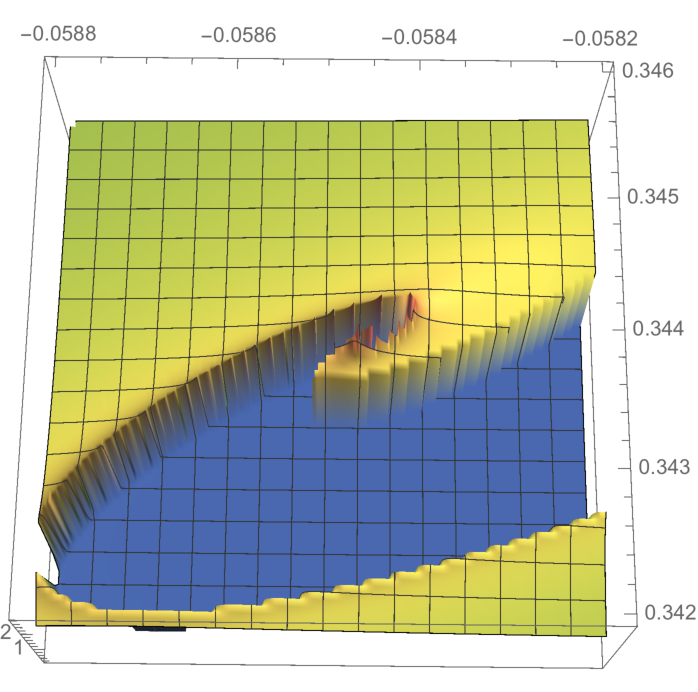
\includegraphics[width=7.5cm]{spike_d3N1.pdf}
  \
  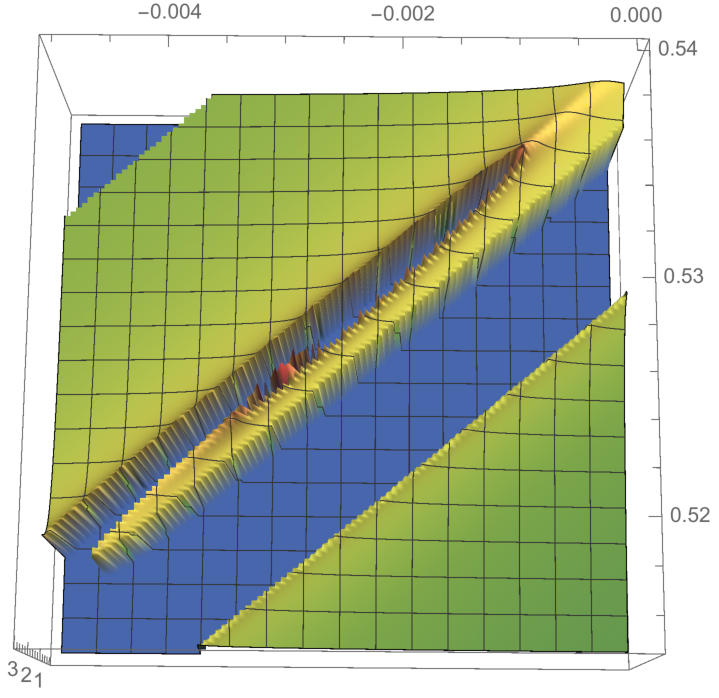
\includegraphics[width=7.5cm]{spike_d3N2.pdf}
  \caption{
    The maximal value of the field reached in the numerical
    evolution before encountering a singularity, as a function
    of the initial conditions $\bV''(\bp=0)$ and $\bF''(\bp=0)$,
    for the case $d=3$ and $\NS=1$ (left panel) and $\NS=2$ (right panel).
    A clear spike can be seen in the centre of each figure.
  }
  \label{WFN1N2}
\end{figure}

% \begin{figure}
%   \begin{tikzpicture}
%     \begin{axis}
%       \addplot3 [surf] table {data/spikeplot1.dat};
%     \end{axis}
%   \end{tikzpicture}
%   % \begin{tikzpicture}
%   %   \begin{axis}
%   %     \addplot3 [surf] gnuplot [raw gnuplot] {
%   %         set dgrid3d 30,30 spline;
%   %       splot 'data/spikeplot1.dat';
%   %   };
%   % \addplot3 [only marks] table {data/spikeplot1.dat};
% % \end{axis}
%   %   \end{tikzpicture}
%   \caption{
%     Does this work?
%   }
% \end{figure}

\noindent For $\NS=2$ the solution can be approximated near the origin by
\begin{align}
  \lim_{\bp \rightarrow 0} \bVstar(\bp) &= 0.014669 - 0.001482 \, \bp ^2 - 0.438516 \, \bp ^4 + 4.35302 \, \bp ^6 + \dots \,, \\
  \lim_{\bp \rightarrow 0} \bFstar(\bp) &= 0.053294 + 0.263370 \, \bp ^2 - 0.570919 \, \bp ^4 + 1.43572 \, \bp ^6 + \dots \,.
\end{align}
The shape of the potential $\bV$ shows that this scaling solution characterises a broken phase.
The asymptotic behaviour of the solution for large $\bp$ is
\begin{align}
  \lim_{\bp \rightarrow \infty} \bVstar(\bp) &= A \bp ^6 + \frac{23}{1440 \pi ^4 B \bp ^2}
                     + \frac{240 \pi ^4 B^2 (16 B+5 \NS-4)-1357 A}{216000 \pi ^6 A B^2 \bp ^4} + \dots \,, \\
  \lim_{\bp \rightarrow \infty} \bFstar(\bp) &= B \bp ^2 + \frac{23}{36 \pi ^2}+\frac{1219}{25920 \pi ^4 B \bp ^2}
                     - \frac{71921 A+2160 \pi ^4 B^2 (16 B+5 \NS-4)}{4665600 \pi ^6 A B^2 \bp ^4} + \dots \,.
\end{align}
For the case $\NS=2$, we were able to establish a very good match between the numerical solution
obtained via shooting methods about the origin and the asymptotic behaviour given above
(setting $A\simeq 5.149$ and $B\simeq 0.273$) about $\bp\simeq0.65$.
We consider this a good candidate for a global scaling solution of the gravitationally
dressed ${\mathrm O(2)}$ scalar model.


\section{The scalar-free cutoff}
\label{sec:purecutoff}

So far we have only considered type-I cutoffs which in the gravitational
sector has the general form $F(\chi^i)R_k(-\bnabla^2)$, where again we denote
the background scalar fields with $\chi^i$.
The presence of the prefactor $F$ is useful because the effect
of adding the cutoff results simply in the replacement of
$-\bnabla^2$ with $P_k(\bnabla^2)=-\bnabla^2+R_k(-\bnabla^2)$
in the Hessians.
However, this advantage comes at a price:
through $F$ the cutoff will depend on running couplings
and there is now an explicit breaking of the scalar split symmetries
$\chi^i \mapsto \chi^i - \epsilon^i$,
$\bp ^i \mapsto \bp ^i + \epsilon^i$, $i=1,\,\dots,\,\NS$, which we discussed in the last chapter.
As shown in Ref. \cite{Bridle:2013sra}, even in pure scalar theory
the presence of the scalar background field
in the cutoff action can lead to unphysical results.
This argument casts doubts on the use of these cutoffs,
and it is therefore important to study cutoffs without
such a prefactor $F$, as well.
In the Einstein-Hilbert truncation, where $F=\nicefrac{1}{16\pi \GNewton}$,
such cutoffs were called ``pure'', \cite{Narain:2009qa}.
Here we shall call them ``scalar-free''.
It is important to keep in mind that any such cutoff will still
depend on the background metric, as we discussed in the last chapter.
% , and that this dependence will
% have to be dealt with by other means, see \eg refs. \cite{Dietz:2015owa,Becker:2014qya}.
Here we only get rid of the $\chi^i$--dependences due to the (matter) scalar fields
and have the scalar msWIs automatically fulfilled.
In particular we shall add in the diagonal entries for $\hTTmunu$
and $\sigma''$ of the Hessian given in Eqn.~(\ref{hessfinal})
a cutoff $\bg \, k^{d-2} \, (k^2-z) \, \theta(k^2-z)$,
with the same sign of the Laplacian term, to implement the coarse-graining procedure.
For all the other terms we shall use the more common
$(k^2-z) \, \theta(k^2-z)$.

We will not report the form of the flow equations in arbitrary dimensions---which
contain hypergeometric functions---but rather focus on the case $d=4$ here only:
\begin{align}
  \dot \bV &= - 4 \bV + \bp \, \bV' - \frac{1}{8\pi^2}
            - \frac{ \bF \left[ \bF (\bV''+1) \log\left( \frac{ 3 \bF'{}^2 }{ \bF (\bV''+1) } + 1 \right) - 3 \bF'{}^2 \right] }
            { 144 \pi^2 \, \bF'{}^4 } \nonumber \\[3mm]
  &         + \frac{ 3 \bg \left[ - \bg^2 + 4\bg \bF - 2\bg(\bg-2\bF) \log \left( \frac{\bF}{\bg} \right) - 3 \bF^2\right]}
                   { 16 \pi ^2 (\bg -\bF)^3}+\frac{(\NS-1) \bp }{32 \pi ^2 \left(\bV'+\bp \right)} \,, \\[5mm]
  \dot \bF &= - 2\bF + \bp \bF' + \frac{19}{384\pi^2}
            + \frac{ \bF \left[\frac{6\bF'^2\left(\bF \bF''+\bF'^2\right)}{3\bF'^2+\bF\left(\bV''+1\right)}
            - \left(2 \bF \bF''+3 \bF'^2\right)
          \log\left(\frac{3 \bF'^2}{\bF(\bV''+1)}+1\right)\right]}{288 \pi ^2 \, \bF'^4} \nonumber \\[3mm]
  &         + \frac{ 10 \bg  (\bg -2 \bF) (\bg -\bF)-5 \bg  \left(\bg ^2-3 \bg  \bF+4 \bF^2\right) \log \left(\frac{\bF}{\bg }\right)}
          { 96 \pi ^2 (\bg -\bF)^3} \nonumber \\[3mm]
  &         + \frac{ \bg\left[-\bg +(\bg-2\bF)\log\left(\frac{\bF}{\bg}\right)+\bF\right]}
                   {96\pi^2(\bg-\bF)^2}
            - \frac{(\NS-1) \bp  \left(3 \bF'+\bV'(\bp )+\bp \right)}{96 \pi ^2 \left(\bV'+\bp\right)^2} \,.
\end{align}
Unlike (\ref{flowvfull}) and (\ref{flowffull}),
these equations are transcendental and cannot be solved analytically.
For comparison, we will discuss scaling solution $\FPone$ only
which was defined via $\bV(\bp)=\bV_0$ and $\bF(\bp)=\bF_0$.
With this ansatz, the fixed point condition reduces to a set of algebraic equations which can be
solved numerically.
% With this ansatz, the fixed point conditions reduce to the following algebraic equations:
% \begin{align}
%   \label{eqnpureFP1-1}
%   \bV_0 &= \frac{1}{128\pi^2(\bg-\bF_0)^2} \bigg[ (\NS-10)\bg^2-2(\NS-13)\bg \bF_0+(\NS-4)\bF_0^2  \nonumber \\
% &\hspace{8cm} -12 \, \bg^2 \, \frac{ \bg - 2\bF_0 }{ \bg - \bF_0} \, \log \left( \frac{\bF_0}{\bg} \right) \bigg] \\[3mm]
%   \label{eqnpureFP1-2}
%   0   &= -2\bF_0-\frac{4N-55}{384\pi^2} -\frac{\bF_0(\bg+9\bF_0)}{96\pi^2(\bg-\bF_0)^2} -\frac{\bg\left(2\bg^2-6\bg \bF_0+9\bF_0^2\right) \log\left(\frac{\bF_0}{\bg}\right)}{48\pi^2(\bg-\bF_0)^3}
% \end{align}
% These can be solved numerically.
The linearisation of the flow equation around $\FPone$ yields the following equations:
\begin{align}
  0 &= - (\lambda+4) \, \deltaV
       - \left[\frac{3\bg\left(3\bF_0^2+5\bg \bF_0-2\bg^2\right)}
                    {16\pi^2\bF_0(\bF_0-\bg)^3}
                  + \frac{3 \bg ^2 (\bg -4\bF_0)}{8\pi^2(\bF_0-\bg)^4}\log\left(\frac{\bF_0}{\bg}\right)\right]\deltaF  \nonumber \\
    &  + \left(\bp-\frac{\NS-1}{32\pi^2\bp}\right)\deltaV'
       - \frac{1}{32\pi^2} \, \deltaV'' \\[3mm]
  0 &= - (\lambda +2) \, \deltaF
       + \left[ \frac{\bg\left(37 \bF_0^2-11\bg \bF_0+4\bg^2\right)}
                    {96\pi^2 \bF_0(\bF_0-\bg)^3}
       - \frac{\bg \bF_0(2\bg+3\bF_0)}{16\pi^2(\bF_0-\bg)^4} \log\left(\frac{\bF_0}{\bg }\right) \right] \deltaF  \nonumber \\
    &  + \left(\bp-\frac{\NS-1}{32\pi^2\bp}\right)\deltaF'
       + \frac{\NS-1}{96\pi^2\bp} \, \deltaV'
       + \frac{1}{96\pi^2} \, \deltaV''
       - \frac{1}{32\pi^2} \, \deltaF''
\end{align}

For $\NS=1$ and $\bg=1$ we have $\bV_{0 \, \star}=0.03314$ and $\bF_{0 \, \star}=0.01552$.
The relevant eigenperturbations around this solution
may be found numerically and the corresponding eigenvalues are given by
$-4$, $-2.272$, $-2$, $-0.272$, $0$.
Therefore, there are four relevant and one marginal coupling.
For $\bg=0.006$ we have $\bV_{0\,\star}=0.00353$ and $\bF_{0\,\star}=0.00670$,
which are very close to the values found with the other cutoff in Ref. \cite{Percacci:2015wwa}.
The relevant eigenperturbations around this solution
have eigenvalues $-4$, $-2.542$, $-2$, $-0.542$, $0$,
which are also closer to the other cutoff.

For $\NS=4$ and $\bg=1$ the fixed point values are given by
$\bV_{0\,\star}=0.03635$ and $\bF_{0\,\star}=0.01413$.
The perturbative analysis around the fixed point gives the following eigenvalues:
$-4$, $-2.299$, $-2$, $-0.299$, $0$.
If instead we were to choose $\bg=0.006$, we had $\bV_{0\,\star}=0.00669$ and $\bF_{0\,\star}=0.00549$,
and the eigenvalues were $-4$, $-2.682$, $-2$, $-0.682$, $0$.

Using the scalar-free cutoff scheme, it is interesting to study solutions to
the fixed point equations for $\FPone$ in the large-$\NS$ limit as well.
It is easy to see that in this limit they assume the following values:
\begin{align}
  \bV_{0 \, \star} \approx \frac{ 16 \NS - 205 }{ 512 \pi^2 } \,, \quad
  \bF_{0 \, \star} \approx \bg\exp{\frac{ 55 - 4 \NS }{16}} \,.
\end{align}
We see that this behaviour is very different from the one obtained previously:
in particular $\bF_{0 \, \star}$ becomes exponentially small but never changes sign.
Thus there is apparently no upper bound in $\NS$ from the requirement of having a positive $\bF_{0 \, \star}$.
This behaviour is induced by the interplay between the logarithmic singularity
in $\bF_{0 \, \star}$ and the linear dependence in $\NS$ in the equations.
This result is probably not physically correct for the following
reason: in the functional renormalisation group one should use the Hessian defined as the second
derivative of the effective average action with respect to the quantum field.
Instead in order to close the flow equation,
we are using the second derivative of the
effective average action with respect to the background field.
Even though the function $F$ does not appear in the cutoff,
it does appear in the denominator, where the coefficient
of $-\bnabla^2$ is $(\bF-\bg) k^{d-2}$.
This term is absent with the type-I cutoff and
it is its presence with the scalar-free cutoff that gives rise
to the logarithmic terms in the flow equation.
In a proper bi-metric calculation the coefficient of
$-\nabla^2$ in the denominator of the functional renormalisation group equation
would be $Z_h-\bg k^{d-2}$, where $Z_h$ is the graviton
wave-function renormalisation.
The argument of the logarithmic term would then be $Z_h/\bg$
and the beta function of $\bF$ would probably be regular for $\bF=0$.



%----------------------------------------------------------------------------------------
% CHAPTER 4
%----------------------------------------------------------------------------------------

\chapter{Dynamics of Matter-Graviton Vertices}
\label{ch:astrid}

The effective average action of a gravitational quantum field theory
at a finite energy scale $k$
depends on both the background as well as the fluctuation field metric,
\ie $\Gamma_k = \Gamma_k[\bar{g}_{\mu \nu}, h_{\mu \nu}]$,
as we have already seen in Ch.~\ref{ch:tim}.
This dependence is such that one cannot recombine $\bar{g}_{\mu \nu}$
and $h_{\mu \nu}$ to give the full metric field,
and modified split Ward identities have to be imposed additionally
to recover split symmetry.
This symmetry breaking is due to two sources:
the gauge fixing term, which gauge-fixes the fluctuations with respect to the background,
as well as the cutoff term, as we have seen already in the case of conformally
reduced gravity in Ch.~\ref{ch:tim}.

As a consequence, couplings of background field operators
do not share the same beta function as the couplings of the fluctuation field operators.
For instance, one could define a Newton coupling from the prefactor of the Einstein-Hilbert term
in the effective action, from the momentum-squared part of the graviton three-point function or
from a graviton-matter vertex.
All of these three definitions of the Newton coupling obey a different renormalisation group running.
Modified Ward-identities govern the background-field dependence of the results,
and have to be imposed on the RG flow,
but using them in practical calculations is still work in its infancy.
We will have a glimpse on how to potentially subtract the background dependence
due to the cutoff term by using these Ward identities in the next chapter.

In the literature on asymptotically safe gravity, many results are obtained within a
single-metric approximation, where the difference between background couplings and fluctuation couplings
is ignored. There, one finds an interacting fixed point with a finite number of relevant couplings,
\ie free parameters, \cf Refs.~\cite{
  Reuter:1996cp, Dou:1997fg, Reuter:2001ag, Lauscher:2001ya, Lauscher:2002sq, Litim:2003vp,
  Fischer:2006fz, Machado:2007ea, Eichhorn:2009ah, Codello:2006in, Codello:2008vh,
  Benedetti:2009rx, Eichhorn:2010tb, Groh:2010ta, Manrique:2011jc, Rechenberger:2012dt, Benedetti:2012dx,
  Dietz:2012ic, Falls:2013bv, Benedetti:2013jk, Ohta:2013uca, Demmel:2014sga, Falls:2014tra, Falls:2015qga,
  Falls:2015cta, Gies:2015tca, Demmel:2015oqa
}.

First explorations of the bi-metric structure in asymptotically safe quantum gravity have indicated that the
evidence for asymptotic safety from the single-metric approximation is still present when
resolving this approximation, \cf Refs.~\cite{
  Manrique:2009uh, Manrique:2010mq, Manrique:2010am, Christiansen:2012rx, Codello:2013fpa,
  Christiansen:2014raa, Becker:2014qya, Christiansen:2015rva
}. One should note that at this stage only a few couplings have been considered in a bi-metric setting,
and higher-order truncations could yield different results.
As discussed in Ref.~\cite{Bridle:2013sra} using the example of a scalar field,
a single-metric approximation can result in spurious fixed points,
and a treatment of the full bi-metric structure is crucial.
Within gravity-matter systems, a first step in this direction has been done in
Refs.~\cite{Dona:2013qba, Dona:2014pla}, where the anomalous dimension of the graviton and matter
fields was evaluated in addition to the beta functions of the gravitational background couplings.
In Refs.~\cite{Christiansen:2014raa, Christiansen:2015rva},
renormalisation group flows formulated in terms of fluctuation field gravitational couplings have been
investigated and lend quantitative support to the results for the pure-gravity
case in the single-metric approximation. The system has been extended to include the effect
of matter fluctuations on pure-gravity-couplings in Ref.~\cite{Meibohm:2015twa}.

In this chapter, we will make a step towards disentangling the running of the fluctuation field and
background field couplings, focusing on the matter-gravity sector.
In the context of asymptotic safety, this implies that a viable fixed point
for the running of the effective average action must not only exist
for the gravitational interactions, but also for matter-gravity interactions and the
matter self-interactions.
As the standard model by itself is most likely not asymptotically safe,
the effect of gravity would have to induce a combined fixed point,
as conjectured in Ref.~\cite{Shaposhnikov:2009pv},
\cf for instance Refs.~\cite{Zanusso:2009bs, Vacca:2010mj,
Harst:2011zx, Eichhorn:2011pc, Eichhorn:2012va,Oda:2015sma
} for evidence in this direction.

As a step towards showing that this could indeed be the case,
we investigate the flow of a gravity-scalar-vertex,
with one external spin-2 gravitational mode and two matter
scalar fields,
and show that it admits an interacting ultraviolet fixed point.
We emphasize that the flow of this coupling is independent from the flow of the usual Newton coupling,
defined with respect to gravitational vertices only.
Our result therefore constitutes non-trivial evidence for the potential viability of asymptotic safety
for a joint description of gravity and matter in our universe.


\section{Matter-gravity flow setup}

In this section we will summaries our setup to study the
non-perturbative renormalisation group flow of the
1-graviton-2-scalar coupling.

\subsection{Truncation}

Our truncation consist of the usual Einstein-Hilbert term for the gravitational sector minimally coupled
to a massless scalar field in the matter sector.
To set it up, we start from an auxiliary action $\hat{\Gamma}_k$ given in terms of the full
metric $\gmunu$, which reads
\begin{align}
  \hat \Gamma_k[\bgmunu, \, \hmunu, \, \varphi] = \int d^4x \, \sqrt{g} \,
  \left[
    - \frac{R}{16 \pi \GNewton} + \frac{1}{2} \, \sum_{i=1}^{\NS} \left( \nabla\varphi^i \right)^2
  \right] .
\end{align}
Note, that this is the same effective average action for $d=4$ as in the previous chapter with
$F=\nicefrac{1}{16\pi\GNewton}$ and $V=0$.
% but with the important difference that all gravitational
% dependences involve the full metric field and not just the background.
We drop a possible volume term in our calculation,
as its fluctuations do not enter the RG flow in our choice of gauge.

As before, we will use the exponential parametrisation of the metric field,
employ a York decomposition for the fluctuation field and use the unimodular physical gauge.
We will specialise our calculation to a flat background $\mathbb R^4$ in four dimensions.
Details of all the involved steps may be found in app. \ref{app:exp_param}.
Since fluctuations of $\xi_\mu$ and $h$ are gauged to zero,
we are left with contributions of $\hTTmunu$ and $\sigma$ to the running couplings.

To calculate the flow, we define a truncation in the following way:
Starting from the action $\hat\Gamma_k$ we expand in powers of $h_{\mu \nu}$ up to fourth order,
and then redefine $h_{\mu \nu} \mapsto \sqrt{32 \pi \GNewton} \, h_{\mu\nu}$.
In the non-perturbative renormalisation group setting,
the running of the couplings of operators at different orders in $h_{\mu \nu}$ may very well differ.
This is why we introduce several different ``avatars'' of the Newton coupling which we denote
by $G_3$, $G_4$, $g_3$, $g_4$ and $g_5$, and define our truncation to be
\begin{align}
  \Gamma_k^\mathrm{rhs} &=
  \sqrt{ \frac{G_3}{\GNewton} \, } \, \hat\Gamma^{(3,\,0)}_k
  + \frac{G_4}{\GNewton} \, \hat\Gamma^{(4,\,0)}_k
  + \sqrt{ \frac{g_3}{\GNewton} \, } \, \hat\Gamma^{(1,\,2)}_k
  + \frac{g_4}{ \GNewton} \, \hat\Gamma^{(2,\,2)}_k
  + \left(\frac{g_5}{ \GNewton}\right)^{3/2} \, \hat\Gamma^{(3,\,2)}_k \nonumber \\
  & + \vphantom{ \sqrt{\frac{g_3}{\GNewton}} }\mbox{ quadratic terms }.
  \label{gammarhs}
\end{align}
Here $\hat \Gamma^{(n,m)}_k$ stands for the terms of $n$-th order in the fluctuation field $h_{\mu \nu}$
and $m$-th order in the scalar field.
Note that the action that contains the scalar fields is quadratic,
so we only have terms with $m=0,2$.
Our redefinition of all separate prefactors of the different vertices allows us to explicitly distinguish
these avatars of the Newton coupling, instead of approximating them all by $\GNewton$.
One should not expect a universal definition of the Newton coupling to exist in the non-perturbative
quantum gravity regime, similarly to what has been found in the perturbative regime in
Ref. \cite{Anber:2011ut}.
As replicas of Newton's coupling, $G_3$, $G_4$, $g_3$, $g_4$ and $g_5$ all have dimensionality $2-d$.
This justifies the different powers with which they appear
in the various terms in our truncation.

In detail, the different terms on a flat background, where we have $\bar{g}_{\mu \nu} = \delta_{\mu \nu}$, are given by:
\begin{alignat}{2}
  &\hat \Gamma^{(3,\, 0)}_k = -\frac{ 2 \, \sqrt{32\pi \GNewton} }{ 3! } &&\int \mathrm d^4x \;
  \bigg[
    \frac{3}{2} \, h_{\mu\nu} \left(\partial_{\mu}h_{\kappa\lambda} \right)\partial_{\nu}h_{\kappa\lambda}
    - 3 \, h_{\kappa \lambda} \left(\partial_{\lambda}h_{\mu\nu} \right)\partial_{\mu}h_{\nu\kappa}
  \bigg] \,, \label{GammaG3} \\
  &\hat \Gamma^{(4,\, 0)}_k = - \frac{ 64\pi \GNewton }{ 4! }  &&\int \mathrm d^4x \;
  \bigg[
    3 \, h_{\mu\nu} \, h_{\kappa\lambda}  \left( \partial_{\mu} h_{\kappa\rho} \right) \partial_{\lambda}h_{\rho\nu}
    - 2 \, h_{\mu\nu} \, h_{\kappa \lambda} \left( \partial_{\lambda} h_{\nu\rho} \right) \partial_{\rho} h_{\mu\kappa} \nonumber \\
    & \hspace{3.8mm} \vphantom{ \frac{ 64\pi \GNewton }{ 4! } } - 3 \, h_{\mu\nu} \, h_{\nu\kappa} \left( \partial_{\kappa} h_{\rho\sigma} \right) && \partial_{\mu}h_{\rho\sigma}
    + 4 \, h_{\mu\nu} \, h_{\nu\kappa} \left( \partial_{\mu} h_{\rho\sigma} \right) \partial_{\sigma} h_{\rho\kappa}
    + \hphantom{3} h_{\nu\kappa} \, h_{\kappa\rho} \left( \partial_{\sigma} h_{\mu\nu} \right) \partial_{\mu} h_{\rho\sigma} \nonumber \\
    & \hspace{3.8mm} \vphantom{ \frac{ 64\pi \GNewton }{ 4! } } + \hphantom{3\,} h_{\mu\nu} \, h_{\kappa\lambda} \left( \partial_{\rho} h_{\mu\kappa} \right) && \partial_{\rho} h_{\nu\lambda}
    - \hphantom{4\, } h_{\mu\nu} \, h_{\nu\kappa} \left(\partial_{\rho} h_{\mu\sigma}\right) \partial_{\rho} h_{\kappa\sigma}
  \bigg] \,, \label{GammaG4}\\
  &\hat \Gamma^{(1,\, 2)}_k = - \frac{\sqrt{32 \pi  \GNewton}}{2}        &&\int \mathrm d^4x \; h^{\mu \nu}  \,
    \sum_{i=1}^{\NS} \partial_{\mu}\varphi^i \, \partial_{\nu}\varphi^i \,, \label{Gammag3} \\
  &\hat \Gamma^{(2,\, 2)}_k = \hphantom{-} \frac{32 \pi  \GNewton}{2}    &&\int \mathrm d^4x \; h^{\mu \rho} \, h_{\rho}^{\phantom{\rho}\nu} \,
    \sum_{i=1}^{\NS} \partial_{\mu}\varphi^i \, \partial_{\nu}\varphi^i \,, \label{Gammag4} \\
  &\hat \Gamma^{(3,\, 2)}_k = - \frac{     (32 \pi  \GNewton)^{3/2}}{2}  &&\int \mathrm d^4x \; h^{\mu \rho} \, h_{\rho}^{\phantom{\rho}\lambda} \, h_{\lambda}^{\phantom{\lambda}\nu}
    \sum_{i=1}^{\NS} \partial_{\mu}\varphi^i \, \partial_{\nu}\varphi^i \,, \label{Gammag5}
\end{alignat}
where appropriate symmetrizations are understood implicitly, as $h_{\mu \nu} = h_{\nu \mu}$.
Here, we have already imposed the gauge $h = \mathrm{const}$,
and thus the trace of the fluctuation field can be dropped from the vertices.
This simplifies the vertices considerably. More details of the derivations of these vertices
in the exponential parametrisation may be found in app. \ref{app:EH}.

In a slight abuse of notation, we will not distinguish between dimensionful and dimensionless couplings in
this chapter,
as all our beta functions will always be expressed in terms of the dimensionless couplings only,
whereas all couplings in Eqns.~\eqref{GammaG3}--\eqref{Gammag5} are still dimensionful.

By the superscript $\mathrm{rhs}$ in \eqref{gammarhs} we indicate that this action is used to define the
vertices and propagators that enter the functional renormalisation group equation.
In other words, these are the fluctuation-field structures that \emph{induce} the renormalization group flow.
In this paper we will not calculate the running of all these couplings, but only the beta function
of $g_3$, and the wave-function renormalisations $Z_\Psi$, where $\Psi = \{ \mathrm{TT}, \, \sigma, \, \mathrm S \}$.
The wave-function renormalisations $Z_\Psi$ nevertheless couple into the beta-functions of the
essential couplings in a non-trivial way via the anomalous dimensions
\begin{align}
  \eta_\Psi = - \partial_t \log Z_\Psi \,.
\end{align}

The running of $G_3$ has been calculated in Ref. \cite{Meibohm:2015twa} using a linear
parametrization of the metric and a more conventional gauge.
We find that the simpler structure of the gravity-matter vertex avoids some of the issues that
are encountered with multi-graviton vertices,
and in any case it is of interest to compare the results of different procedures.

The coupled nature of the functional renormalisation group equation clearly prevents
us from defining a closed truncation,
in which we can extract the flow of all couplings that we have included on the right-hand side;
thus approximations are necessary in which some couplings contribute to the running of others,
but their running is not calculated.
The remaining couplings in (\ref{gammarhs}) can accordingly be treated in various ways.
Since they enter in the flow equation for $g_3$,
it is better to avoid a truncation where they are set to zero.
Instead, they can be set equal to $g_3$, or treated as free parameters.
We will discuss different possible approximations with respect to these higher-order couplings below.
It is important to realize that if we were to restrict our truncation to $g_3$,
and set all other couplings to zero,
all but diagrams 4 and 5 in Fig.~\ref{fig:coupling-diagrams-ch4} would vanish.
On the other hand, the original action is diffeomorphism invariant,
and accordingly a 1-graviton-2-scalar-vertex is necessarily accompanied by a 2-graviton-2-scalar vertex etc.
It is therefore expected that an improved truncation takes the existence of these couplings---and
the corresponding diagrams---into account.
To close the system of couplings, we clearly have to choose an approximation,
and we will mostly opt for the choice $g_3=g_4=g_5$ in the following
(which is dictated by dimensionality). To check how useful this approximation is,
we will keep track of all couplings separately;
however, we will not evaluate the flows of higher-order couplings.

Note an interesting difference of $\beta_{g_3}$ to the running of the background Newton coupling:
As there is no closed scalar loop contributing to $\beta_{g_3}$,
its only dependence on $\NS$ arises through the anomalous dimension $\etaTT$.


\subsection{Projection rules}

We use the transverse traceless mode $\hTTmunu$
to define the matter-gravity coupling $g_3$.
Then the running of $g_3$ can be extracted unambiguously on a flat background.
To do this, we employ a projection rule as follows:
\begin{align}
  \partial_t \sqrt{g_3} = \frac{8}{3} \, \frac{1}{\sqrt{32 \pi}} \,
  \left(
    p_{1\mu} \, p_{2\nu}  \,
    \frac{\delta}{\delta \hTTmunu(p_3)} \, \frac{\delta}{\delta\varphi(p_1)} \, \frac{\delta}{\delta\varphi(p_2)} \,
    \partial_t \hat \Gamma_k
  \right) \bigg|_{(p^2)^2} \,,
  \label{projectiong3}
\end{align}
where we use the symmetric configuration for the three momenta,
such that an angle of $2\pi/3$ lies between them, and their absolute value is $|p_1| = |p_2|=|p_3| =p$.
Note that the functional derivative with respect to the $\mathrm{TT}$ mode generates the projector
\begin{align}
  \mathcal{P}^{\rm TT}_{\mu\nu\kappa\lambda} = \frac{1}{2} \,
  \left(
    T_{\mu
    \kappa}T_{\nu \lambda}
    + T_{\mu\lambda}T_{\nu \kappa}
  \right)
  - \frac{1}{d-1} \, T_{\mu\nu}T_{\kappa\lambda},
  \label{projector}
\end{align}
where $T_{\mu \nu}=\delta_{\mu\nu}-p_{\mu}p_{\nu}/p^2$.
As we are using the transverse traceless component of the graviton for the projection,
there is no mixing with non-minimal couplings that arise from the diffeomorphism-invariant
operator $\varphi^2 R$, since the first variation of $R$ does not have a transverse traceless
component  on a flat background.
Furthermore, working with a transverse traceless external graviton mode also excludes an admixture
of non-diffeomorphism invariant operators at the same order of momenta,
which might be generated by the flow and which depend on the momenta of the graviton.

Any given vertex contains a large number of different tensor structures,
and these are not necessarily all featuring the same running coupling.
In particular, transverse traceless structures and scalar structures could be expected to exhibit
prominent differences in their running. As a first step into this direction,
we distinguish the wave-function renormalization for the $\mathrm{TT}$ mode and the $\sigma$ mode,
$\ZTT$ and $Z_{\sigma}$. On the other hand, we do not distinguish the couplings in the same fashion.

To extract the flow of the wave-function renormalisations, we define projection rules as follows:
\begin{align}
  \partial_t \ZS &=
  \frac{\partial}{\partial p^2} \, \frac{\delta}{\delta \varphi(-p)} \, \frac{\delta}{\delta \varphi(p)} \, \partial_t \hat \Gamma_k \,, \\
  \partial_t \ZTT &=
  \frac{\partial}{\partial p^2}  \, \frac{\mathcal P^{\TT}_{\mu \nu\kappa\lambda}(p)}{5}  \, \frac{\delta^2}{\delta \hTTmunu (p) \, \delta h^{\TT}_{\kappa \lambda}(-p)} \, \partial_t \hat \Gamma_k \,, \\
  \partial_t Z_{\sigma} &= -\frac{8}{3} \,
  \frac{\partial}{\partial p^2} \, \frac{\delta}{\delta \sigma(-p)} \, \frac{\delta}{\delta \sigma(p)} \, \partial_t \hat \Gamma_k \,,
\end{align}
where the right-hand sides are evaluated at $p=0$,
and at vanishing external fields $\hTTmunu$, $\sigma$ and $\varphi$.


\section{Results for beta functions and anomalous dimensions}

For our explicit results, we will employ a regulator shape function of the form
\begin{align}
  \nonumber
  R_{\Psi k} \left( p^2\right) = Z_{\Psi k} \, (p^2-k^2) \, \theta(k^2-p^2) \,,
\end{align}
with the appropriate wave-function renormalization for all modes, \cf Ref.~\cite{Litim:2001up}.


\subsection{The anomalous dimensions}

\begin{figure}[p]
  \begin{center}
    \begin{tikzpicture}[
    >=stealth,
    scale=1.00,
    thick,
    % very thick,
  ]

  \tikzmath{
    \radius    = 0.72; % radius of right circle
    \dotradius = 0.07; % radius of the circles that make the dots
  }

  % define the distances between the Feynman diagrams
  \coordinate  (dist5) at ( 0.0,  0.0);
  \coordinate  (dist3) at ( 3.5,  0.0);
  \coordinate  (dist4) at ( 7.0,  0.0);
  \coordinate  (dist7) at (10.5,  0.0);

  \coordinate  (dist1) at ( 0.0, -3.0);
  \coordinate  (dist2) at ( 3.5, -3.0);
  \coordinate  (dist6) at ( 7.0, -3.0);

  \coordinate (dist10) at ( 0.0, -6.5);
  \coordinate (dist11) at ( 3.5, -6.5);
  \coordinate  (dist8) at ( 7.0, -6.5);
  \coordinate  (dist9) at (10.5, -6.5);

  \draw (  -2, -4.75) -- (12.25, -4.75);
  \draw (  -2,  1.5)  -- (   -2, -8.25);
  \draw (12.25, 1.5)  -- (12.25, -8.25);
  \draw (  -2,  1.5)  -- (12.25, 1.5);
  \draw (  -2, -8.25) -- (12.25, -8.25);

  %--------------
  %  DIAGRAM 1  |
  %--------------

  % Loop composet out of circle with annotation
  \draw[TT]   ($ (dist1) + (0, -\radius) $) arc (-90:270:\radius);
  \draw[TT]   ($ (dist1) + (0,  \radius) $) node[above, inner sep=2mm] {$\hTT$};

  % Two external legs pointing outwards at bottom
  \draw[TT]   ($ (dist1) + (-0.72*\radius, -1.97*\radius) $) -- ($ (dist1) + (0, -\radius)$)
    node[left, midway, inner sep=3mm] {$\hTT$};
  \draw[TT]   ($ (dist1) + ( 0.72*\radius, -1.97*\radius) $) -- ($ (dist1) + (0, -\radius)$)
    node[right, midway, inner sep=3mm] {$\hTT$};

  % One dot for vertex
  \draw[fill] ($ (dist1) + (0, -\radius)                $) circle [radius=\dotradius];

  % Number of diagram
  \draw       ($ (dist1) + (-1.5*\radius,  1.5*\radius) $) node[] {$\boxed{5}$};

  %--------------
  %  DIAGRAM 2  |
  %--------------

  % Loop composet out of circle with annotation
  \draw[sigma] ($ (dist2) + (0, -\radius) $) arc (-90:270:\radius);
  \draw[sigma] ($ (dist2) + (0,  \radius) $) node[above, inner sep=2mm] {$\sigma$};

  % Two external legs pointing outwards at bottom
  \draw[TT]   ($ (dist2) + (-0.72*\radius, -1.97*\radius) $) -- ($ (dist2) + (0, -\radius)$)
    node[left, midway, inner sep=3mm] {$\hTT$};
  \draw[TT]   ($ (dist2) + ( 0.72*\radius, -1.97*\radius) $) -- ($ (dist2) + (0, -\radius)$)
    node[right, midway, inner sep=3mm] {$\hTT$};

  % One dot for vertex
  \draw[fill] ($ (dist2) + (0, -\radius)                $) circle [radius=\dotradius];

  % Number of diagram
  \draw       ($ (dist2) + (-1.5*\radius,  1.5*\radius) $) node[] {$\boxed{6}$};

  %--------------
  %  DIAGRAM 3  |
  %--------------

  % Loop composed out of two segments + annotation
  \draw[sigma] ($ (dist3) + (-\radius, 0) $) arc (180:   0: \radius);
  \draw[TT]    ($ (dist3) + (-\radius, 0) $) arc (180: 360: \radius);
  \draw        ($ (dist3) + (0,  \radius) $) node[above, inner sep=2mm] {$\sigma$};
  \draw        ($ (dist3) + (0, -\radius) $) node[below, inner sep=2mm] {$\hTT$};

  % Two horizontal external legs
  \draw[TT]    ($ (dist3) + (2.1*\radius, 0) $) -- ($ (dist3) + (     \radius, 0) $)
    node[above, midway, inner sep=2mm] {$\hTT$};
  \draw[TT]    ($ (dist3) + (   -\radius, 0) $) -- ($ (dist3) + (-2.1*\radius, 0) $)
    node[above, midway, inner sep=2mm] {$\hTT$};

  % Two dots for vertices
  \draw[fill]  ($ (dist3) + (-\radius, 0) $) circle [radius=\dotradius];
  \draw[fill]  ($ (dist3) + ( \radius, 0) $) circle [radius=\dotradius];

  % Number of diagram
  \draw        ($ (dist3) + (-1.5*\radius,  1.5*\radius) $) node[] {$\boxed{2}$};

  %--------------
  %  DIAGRAM 4  |
  %--------------

  % Loop composed out of two segments + annotation
  \draw[sigma] ($ (dist4) + (-\radius, 0) $) arc (180:   0: \radius);
  \draw[sigma] ($ (dist4) + (-\radius, 0) $) arc (180: 360: \radius);
  \draw        ($ (dist4) + (0,  \radius) $) node[above, inner sep=2mm] {$\sigma$};
  \draw        ($ (dist4) + (0, -\radius) $) node[below, inner sep=2mm] {$\sigma$};

  % Two horizontal external legs
  \draw[TT]    ($ (dist4) + (2.1*\radius, 0) $) -- ($ (dist4) + (     \radius, 0) $)
    node[above, midway, inner sep=2mm] {$\hTT$};
  \draw[TT]    ($ (dist4) + (   -\radius, 0) $) -- ($ (dist4) + (-2.1*\radius, 0) $)
    node[above, midway, inner sep=2mm] {$\hTT$};

  % Two dots for vertices
  \draw[fill]  ($ (dist4) + (-\radius, 0) $) circle [radius=\dotradius];
  \draw[fill]  ($ (dist4) + ( \radius, 0) $) circle [radius=\dotradius];

  % Number of diagram
  \draw        ($ (dist4) + (-1.5*\radius,  1.5*\radius) $) node[] {$\boxed{3}$};

  %--------------
  %  DIAGRAM 5  |
  %--------------

  % Loop composed out of two segments + annotation
  \draw[TT]    ($ (dist5) + (-\radius, 0) $) arc (180:   0: \radius);
  \draw[TT]    ($ (dist5) + (-\radius, 0) $) arc (180: 360: \radius);
  \draw        ($ (dist5) + (0,  \radius) $) node[above, inner sep=2mm] {$\hTT$};
  \draw        ($ (dist5) + (0, -\radius) $) node[below, inner sep=2mm] {$\hTT$};

  % Two horizontal external legs
  \draw[TT]    ($ (dist5) + (2.1*\radius, 0) $) -- ($ (dist5) + (     \radius, 0) $)
    node[above, midway, inner sep=2mm] {$\hTT$};
  \draw[TT]    ($ (dist5) + (   -\radius, 0) $) -- ($ (dist5) + (-2.1*\radius, 0) $)
    node[above, midway, inner sep=2mm] {$\hTT$};

  % Two dots for vertices
  \draw[fill]  ($ (dist5) + (-\radius, 0) $) circle [radius=\dotradius];
  \draw[fill]  ($ (dist5) + ( \radius, 0) $) circle [radius=\dotradius];

  % Number of diagram
  \draw        ($ (dist5) + (-1.5*\radius,  1.5*\radius) $) node[] {$\boxed{1}$};

  %--------------
  %  DIAGRAM 6  |
  %--------------

  % Loop composet out of circle with annotation
  \draw        ($ (dist6) + (0, -\radius) $) arc (-90:270:\radius);
  \draw        ($ (dist6) + (0,  \radius) $) node[above, inner sep=2mm] {$\phi$};

  % Two external legs pointing outwards at bottom
  \draw[TT]    ($ (dist6) + (-0.72*\radius, -1.97*\radius) $) -- ($ (dist6) + (0, -\radius)$)
    node[left, midway, inner sep=3mm] {$\hTT$};
  \draw[TT]    ($ (dist6) + ( 0.72*\radius, -1.97*\radius) $) -- ($ (dist6) + (0, -\radius)$)
    node[right, midway, inner sep=3mm] {$\hTT$};

  % One dot for vertex
  \draw[fill]  ($ (dist6) + (0, -\radius)                $) circle [radius=\dotradius];

  % Number of diagram
  \draw        ($ (dist6) + (-1.5*\radius,  1.5*\radius) $) node[] {$\boxed{7}$};

  %--------------
  %  DIAGRAM 7  |
  %--------------

  % Loop composed out of two segments + annotation
  \draw        ($ (dist7) + (-\radius, 0) $) arc (180:   0: \radius);
  \draw        ($ (dist7) + (-\radius, 0) $) arc (180: 360: \radius);
  \draw        ($ (dist7) + (0,  \radius) $) node[above, inner sep=2mm] {$\phi$};
  \draw        ($ (dist7) + (0, -\radius) $) node[below, inner sep=2mm] {$\phi$};

  % Two horizontal external legs
  \draw[TT]    ($ (dist7) + (2.1*\radius, 0) $) -- ($ (dist7) + (     \radius, 0) $)
    node[above, midway, inner sep=2mm] {$\hTT$};
  \draw[TT]    ($ (dist7) + (   -\radius, 0) $) -- ($ (dist7) + (-2.1*\radius, 0) $)
    node[above, midway, inner sep=2mm] {$\hTT$};

  % Two dots for vertices
  \draw[fill]  ($ (dist7) + (-\radius, 0) $) circle [radius=\dotradius];
  \draw[fill]  ($ (dist7) + ( \radius, 0) $) circle [radius=\dotradius];

  % Number of diagram
  \draw        ($ (dist7) + (-1.5*\radius,  1.5*\radius) $) node[] {$\boxed{4}$};

  %--------------
  %  DIAGRAM 8  |
  %--------------

  % Loop composet out of circle with annotation
  \draw[TT]   ($ (dist8) + (0, -\radius) $) arc (-90:270:\radius);
  \draw[TT]   ($ (dist8) + (0,  \radius) $) node[above, inner sep=2mm] {$\hTT$};

  % Two external legs pointing outwards at bottom
  \draw       ($ (dist8) + (-0.72*\radius, -1.97*\radius) $) -- ($ (dist8) + (0, -\radius)$)
    node[left, midway, inner sep=3mm] {$\phi$};
  \draw       ($ (dist8) + ( 0.72*\radius, -1.97*\radius) $) -- ($ (dist8) + (0, -\radius)$)
    node[right, midway, inner sep=3mm] {$\phi$};

  % One dot for vertex
  \draw[fill] ($ (dist8) + (0, -\radius)                $) circle [radius=\dotradius];

  % Number of diagram
  \draw       ($ (dist8) + (-1.5*\radius,  1.5*\radius) $) node[] {$\boxed{5^\prime}$};

  %--------------
  %  DIAGRAM 9  |
  %--------------

  % Loop composet out of circle with annotation
  \draw[sigma] ($ (dist9) + (0, -\radius) $) arc (-90:270:\radius);
  \draw[sigma] ($ (dist9) + (0,  \radius) $) node[above, inner sep=2mm] {$\sigma$};

  % Two external legs pointing outwards at bottom
  \draw       ($ (dist9) + (-0.72*\radius, -1.97*\radius) $) -- ($ (dist9) + (0, -\radius)$)
    node[left, midway, inner sep=3mm] {$\phi$};
  \draw       ($ (dist9) + ( 0.72*\radius, -1.97*\radius) $) -- ($ (dist9) + (0, -\radius)$)
    node[right, midway, inner sep=3mm] {$\phi$};

  % One dot for vertex
  \draw[fill] ($ (dist9) + (0, -\radius)                $) circle [radius=\dotradius];

  % Number of diagram
  \draw       ($ (dist9) + (-1.5*\radius,  1.5*\radius) $) node[] {$\boxed{6^\prime}$};

  %--------------
  %  DIAGRAM 10  |
  %--------------

  % Loop composed out of two segments + annotation
  \draw[TT]    ($ (dist10) + (-\radius, 0) $) arc (180:   0: \radius);
  \draw        ($ (dist10) + (-\radius, 0) $) arc (180: 360: \radius);
  \draw        ($ (dist10) + (0,  \radius) $) node[above, inner sep=2mm] {$\hTT$};
  \draw        ($ (dist10) + (0, -\radius) $) node[below, inner sep=2mm] {$\phi$};

  % Two horizontal external legs
  \draw        ($ (dist10) + (2.1*\radius, 0) $) -- ($ (dist10) + (     \radius, 0) $)
    node[above, midway, inner sep=2mm] {$\phi$};
  \draw        ($ (dist10) + (   -\radius, 0) $) -- ($ (dist10) + (-2.1*\radius, 0) $)
    node[above, midway, inner sep=2mm] {$\phi$};

  % Two dots for vertices
  \draw[fill]  ($ (dist10) + (-\radius, 0) $) circle [radius=\dotradius];
  \draw[fill]  ($ (dist10) + ( \radius, 0) $) circle [radius=\dotradius];

  % Number of diagram
  \draw        ($ (dist10) + (-1.5*\radius,  1.5*\radius) $) node[] {$\boxed{1^\prime}$};

  %--------------
  %  DIAGRAM 11  |
  %--------------

  % Loop composed out of two segments + annotation
  \draw[sigma] ($ (dist11) + (-\radius, 0) $) arc (180:   0: \radius);
  \draw        ($ (dist11) + (-\radius, 0) $) arc (180: 360: \radius);
  \draw        ($ (dist11) + (0,  \radius) $) node[above, inner sep=2mm] {$\sigma$};
  \draw        ($ (dist11) + (0, -\radius) $) node[below, inner sep=2mm] {$\phi$};

  % Two horizontal external legs
  \draw        ($ (dist11) + (2.1*\radius, 0) $) -- ($ (dist11) + (     \radius, 0) $)
    node[above, midway, inner sep=2mm] {$\phi$};
  \draw        ($ (dist11) + (   -\radius, 0) $) -- ($ (dist11) + (-2.1*\radius, 0) $)
    node[above, midway, inner sep=2mm] {$\phi$};

  % Two dots for vertices
  \draw[fill]  ($ (dist11) + (-\radius, 0) $) circle [radius=\dotradius];
  \draw[fill]  ($ (dist11) + ( \radius, 0) $) circle [radius=\dotradius];

  % Number of diagram
  \draw        ($ (dist11) + (-1.5*\radius,  1.5*\radius) $) node[] {$\boxed{2^\prime}$};

\end{tikzpicture}

  \end{center}
  \caption{
    Diagrams which contribute to the running of the anomalous dimensions
    $\etaTT$ (first two rows) and $\etaS$ (third~row).
    Diagrams similar to the once in the first two rows, but with external $\sigma$ legs,
    contribute to the running of the anomalous dimension $\eta_{\sigma}$.
  }
  \label{fig:eta-diagrams-ch4}
\end{figure}

{
  \setlength{\extrarowheight}{10pt}
  \begin{table}[p]
    \begin{center}
      \begin{tabular}{ l@{\hskip 5mm} r@{\hskip 7mm} r@{\hskip 7mm} r }
        \toprule
        diagram        &  $\etaTT$ & $\eta_\sigma$ & $\etaS$ \\
        \midrule
        1 / 1$^\star$  &  $\displaystyle -\frac{5 \, G_3}{864 \pi} \, \big( 388-53\etaTT \big)$
                       &  $\displaystyle \frac{5 \,  G_3}{432\pi} \, \big(40-23\etaTT \big)$
                       &  $0$                                              \\
        2 / 2$^\star$  &  $\displaystyle \frac{25 \, G_3}{576 \pi} \, \big(16-\etaTT-\eta_{\sigma} \big)$
                       &  $\displaystyle - \frac{5 \,  G_3}{144\pi} \, \big(16-\etaTT- \eta_{\sigma} \big)$
                       &  $\displaystyle \frac{g_3}{16\pi} \, \big(16-\eta_{\sigma}-\etaS \big)$ \\
        3              &  $\displaystyle -\frac{G_3}{216 \pi} \, \big(31-5\eta_{\sigma} \big)$
                       &  $\displaystyle \frac{G_3}{432\pi} \, \big(136 - 35 \eta_{\sigma} \big)$
                       &  ---                                              \\
        4              &  $\displaystyle \frac{\NS \, g_3}{24 \pi}$
                       &  $\displaystyle \frac{\NS \, g_3}{48 \pi} \, \big(8-3\etaS \big)$
                       &  ---                                              \\
        5 / 5$^\star$  &  $\displaystyle \frac{145 \, G_4}{648 \pi} \, \big(6-\etaTT  \big)$
                       &  $\displaystyle \frac{55 \, G_4}{648 \pi}\big(6-\etaTT \big)$
                       &  $\displaystyle \frac{5 \ g_4}{24\pi} \, \big(6-\etaTT \big)$            \\
        6 / 6$^\star$  &  $\displaystyle -\frac{29 \, G_4}{324 \pi} \, \big(6-\eta_{\sigma} \big)$
                       &  $\displaystyle -\frac{11 \, G_4}{324 \pi} \big(6-\eta_{\sigma} \big)$
                       &  $\displaystyle -\frac{g_4}{12 \pi} \, \big(6-\eta_{\sigma} \big)$       \\
        7              &  $0$
                       &  $0$
                       &  ---                                              \\
        \bottomrule
      \end{tabular}
    \end{center}
    \caption[Coordinates and critical exponents of fixed points in perturbative approximation]
    {
      All individual contributions to the anomalous dimensions $\etaTT$, $\eta_\sigma$ and $\etaS$
      contributing due to the diagrams displayed in Fig. \ref{fig:eta-diagrams-ch4} above.
    }
    \label{tab:eta-results}
  \end{table}
}

To extract the running of the anomalous dimensions, we had to evaluate 18 diagrams, 7 for
each of the gravitational modes and 4 for the matter scalar. We display the types of
diagrams arising for the $\mathrm{TT}$ mode and for $\varphi$ on the next page in
Fig.~\ref{fig:eta-diagrams-ch4}.
Actually, each diagram displayed there is the sum of $n$ different terms,
where each summand is the same diagram, except that it carries an additional regulator,
inserted in exactly one of the $n$ propagators. We also present the analytic results for
each of these diagrams on the same page in Tab.~\ref{tab:eta-results}.

Summing all contributions given in the table, we obtain the following results:
\begin{align}
  \etaTT      &= \frac{\NS \, g_3}{24 \pi} - \frac{G_3}{1728 \pi} \big( 2928 - 455 \etaTT + 35 \eta_\sigma \big)
  + \frac{29 \, G_4}{648 \pi} \big( 18 - 5 \etaTT + 2 \eta_\sigma \big) \,,
  \label{etaTTcomplete} \\
  \eta_\sigma &= \frac{\NS \, g_3}{48 \pi} \big( 8-3 \etaS \big) + \frac{G_3}{108 \pi} \big( 24 - 25\etaTT - 5 \eta_\sigma \big)
   +\frac{11 \, G_4}{648 \pi} \big( 18 - 5 \etaTT + 2 \eta_\sigma \big) \,,
  \label{etasigmacomplete} \\
  \etaS &= \frac{g_3}{16\pi} \, \big(16-\eta_{\sigma}-\etaS \big)
  + \frac{g_4}{24 \pi} \, \big( 18 - 5 \etaTT + 2 \eta_{\sigma} \big) \,.
\end{align}
Note that the sign of the matter contribution agrees for $\etaTT$ and $\eta_\sigma$
and is the opposite one from that in the linear parametrization and de~Donder gauge,
\cf Ref.~\cite{Dona:2013qba}. Since the exponential parametrization and the linear parametrization
can be understood as underlying two distinct definitions of the configuration space for
asymptotically safe quantum gravity, such a difference could possibly persist in extended truncations,
and points towards a difference in the number of relevant directions in the two settings,
\cf also Ref.~\cite{Ohta:2015efa}.

The two-vertex diagrams (first row in Fig.~\ref{fig:eta-diagrams-ch4})
enter with opposite signs in $\etaTT$ as compared to $\eta_\sigma$.
This will imply that the two anomalous dimensions will typically have values of similar magnitude
but opposite sign. Thus, setting $\eta_\sigma = \etaTT$ does not seem to be a good approximation,
if indeed this trend persists beyond our truncation.
Moreover, this could suggest that even in calculations without a York decomposition,
it might be necessary to disentangle the tensor structures of the graviton,
and work with projection tensors.
Comparing to the anomalous dimension $\eta_h$ for the graviton (without York decomposition)
in the linear parametrization, we observe that $\etaTT$ has the opposite,
leading order \emph{negative} contribution from the pure-gravity fluctuations,
\cf Eqn.~(24) in Ref.~\cite{Dona:2013qba}.

There are only four diagrams contributing to the flow of $\etaS$, two tadpole diagrams and two two-vertex diagrams,
\cf the third row in Fig.~\ref{fig:eta-diagrams-ch4}.
Overall, $\etaS$ is positive at leading order, when $g_3>0, g_4>0$.
This is the opposite behaviour as that observed in the linear parametrization
and the de~Donder gauge, \cf Ref.~\cite{Dona:2013qba}.


\subsection{The flow of the graviton-matter coupling}

There are 12 diagrams contributing to the
flow of the 1-graviton-2-scalar-vertex
which together with there analytical values can be found on
the next page
% page \pageref{fig:coupling-diagrams-ch4}.
in Fig.~\ref{fig:coupling-diagrams-ch4} and Tab.~\ref{tab:coupling-diagrams-ch4},
respectively.


The flow of $\sqrt{g_3}$ is driven by three types of diagrams.
First of all, there are three-vertex diagrams in which all
vertices are proportional to $\sqrt{g_3}$ themselves,
namely diagrams 4 and 5.
We do not distinguish between the coupling of two
scalars and one $\sigma$ mode and the coupling of two scalars and
the $\mathrm{TT}$ mode,
although we use only the latter to read off the running of $g_3$.
Note that diagrams 4 and 5 do not get contributions from the $\mathrm{TT}$ mode;
the transverse traceless mode contributes to the running of the
1-graviton-2-scalar-vertex only at a higher order in the momenta,
when our projection prescription \eqref{projectiong3} is used.
The leading-order contribution to the beta function coming from
these diagrams has a positive sign.

The other two types of diagrams are the tadpole diagrams 11 and 12
and the two-vertex diagrams 6--10.
They contain the couplings $g_4$ and $g_5^{3/2}$ and
some of them (diagrams 9--12) exclusively arise from the kinetic term of the scalar.
The two tadpole diagrams contribute at $\mathcal{O}(g_5^{3/2})$ to the flow of $g_3$.
The two-vertex diagrams 9 and 10 contain only gravity-matter vertices and contribute
at $\mathcal{O}(\sqrt{g_3} g_4)$ to the flow of $\sqrt{g_3}$.
Finally, there are two-and three-vertex diagrams (diagrams 1--3 and 6--8)
which contain the vertex $\sqrt{G_3}$, arising from the Einstein-Hilbert action.

\begin{figure}[p]
  \begin{center}
    \begin{tikzpicture}[
    >=stealth,
    scale=1.00,
    thick,
    % very thick,
  ]

  \tikzmath{
    \radius    = 0.72; % radius of right circle
    \dotradius = 0.07; % radius of the circles that make the dots
  }

  % define the distances between the Feynman diagrams
  \coordinate   (dist1) at ( 0.0,  0.0);
  \coordinate   (dist2) at ( 3.5,  0.0);
  \coordinate   (dist3) at ( 7.0,  0.0);
  \coordinate   (dist4) at (10.5,  0.0);

  \coordinate   (dist5) at ( 0.0, -3.0);
  \coordinate   (dist6) at ( 3.5, -3.0);
  \coordinate   (dist7) at ( 7.0, -3.0);
  \coordinate   (dist8) at (10.5, -3.0);

  \coordinate   (dist9) at ( 0.0, -6.0);
  \coordinate  (dist10) at ( 3.5, -6.0);
  \coordinate  (dist11) at ( 7.0, -6.0);
  \coordinate  (dist12) at (10.5, -6.0);

  \draw (  -2,  1.5)  -- (   -2, -7.75);
  \draw (12.25, 1.5)  -- (12.25, -7.75);
  \draw (  -2,  1.5)  -- (12.25, 1.5);
  \draw (  -2, -7.75) -- (12.25, -7.75);

  %--------------
  %  DIAGRAM 1  |
  %--------------

  % External leg incoming from the left
  \draw[TT]    ($ (dist1) + (-2.1*\radius, 0.0*\radius) $) -- ($ (dist1) + (-1.0*\radius,  0*\radius) $)
    node[above, near start, inner sep=2mm] {$\hTT$};

  % Triangle loop: going up, going down, vertical
  \draw[TT]    ($ (dist1) + (-1.0*\radius, 0.0*\radius) $) -- ($ (dist1) + ( 0.6*\radius,  1*\radius) $)
    node[above, near start, inner sep=3mm] {$\hTT$};
  \draw[TT]    ($ (dist1) + (-1.0*\radius, 0.0*\radius) $) -- ($ (dist1) + ( 0.6*\radius, -1*\radius) $)
    node[below, near start, inner sep=2mm] {$\hTT$};
  \draw        ($ (dist1) + ( 0.6*\radius, 1.0*\radius) $) -- ($ (dist1) + ( 0.6*\radius, -1*\radius) $)
    node[right, midway, inner sep=2mm] {$\phi$};

  % Two external legs incoming from the right: above, below
  \draw        ($ (dist1) + ( 0.6*\radius, 1.0*\radius) $) -- ($ (dist1) + ( 1.7*\radius,  1*\radius) $)
    node[above, near end, inner sep=1mm] {$\phi$};
  \draw        ($ (dist1) + ( 0.6*\radius,-1.0*\radius) $) -- ($ (dist1) + ( 1.7*\radius, -1*\radius) $)
    node[below, near end, inner sep=1mm] {$\phi$};

  % Three dots for the vertices
  \draw[fill]  ($ (dist1) + (-1.0*\radius, 0.0*\radius) $) circle [radius=\dotradius];
  \draw[fill]  ($ (dist1) + ( 0.6*\radius, 1.0*\radius) $) circle [radius=\dotradius];
  \draw[fill]  ($ (dist1) + ( 0.6*\radius,-1.0*\radius) $) circle [radius=\dotradius];

  % Number of diagram
  \draw        ($ (dist1) + (-1.5*\radius, 1.5*\radius) $) node[] {$\boxed{1}$};

  %--------------
  %  DIAGRAM 2  |
  %--------------

  % External leg incoming from the left
  \draw[TT]    ($ (dist2) + (-2.1*\radius, 0.0*\radius) $) -- ($ (dist2) + (-1.0*\radius,  0*\radius) $)
    node[above, near start, inner sep=2mm] {$\hTT$};

  % Triangle loop: going up, going down, vertical
  \draw[TT]    ($ (dist2) + (-1.0*\radius, 0.0*\radius) $) -- ($ (dist2) + ( 0.6*\radius,  1*\radius) $)
    node[above, near start, inner sep=3mm] {$\hTT$};
  \draw[sigma] ($ (dist2) + (-1.0*\radius, 0.0*\radius) $) -- ($ (dist2) + ( 0.6*\radius, -1*\radius) $)
    node[below, near start, inner sep=2mm] {$\sigma$};
  \draw        ($ (dist2) + ( 0.6*\radius, 1.0*\radius) $) -- ($ (dist2) + ( 0.6*\radius, -1*\radius) $)
    node[right, midway, inner sep=2mm] {$\phi$};

  % Two external legs incoming from the right: above, below
  \draw        ($ (dist2) + ( 0.6*\radius, 1.0*\radius) $) -- ($ (dist2) + ( 1.7*\radius,  1*\radius) $)
    node[above, near end, inner sep=1mm] {$\phi$};
  \draw        ($ (dist2) + ( 0.6*\radius,-1.0*\radius) $) -- ($ (dist2) + ( 1.7*\radius, -1*\radius) $)
    node[below, near end, inner sep=1mm] {$\phi$};

  % Three dots for the vertices
  \draw[fill]  ($ (dist2) + (-1.0*\radius, 0.0*\radius) $) circle [radius=\dotradius];
  \draw[fill]  ($ (dist2) + ( 0.6*\radius, 1.0*\radius) $) circle [radius=\dotradius];
  \draw[fill]  ($ (dist2) + ( 0.6*\radius,-1.0*\radius) $) circle [radius=\dotradius];

  % Number of diagram
  \draw        ($ (dist2) + (-1.5*\radius, 1.5*\radius) $) node[] {$\boxed{2}$};

  %--------------
  %  DIAGRAM 3  |
  %--------------

  % External leg incoming from the left
  \draw[TT]    ($ (dist3) + (-2.1*\radius, 0.0*\radius) $) -- ($ (dist3) + (-1.0*\radius,  0*\radius) $)
    node[above, near start, inner sep=2mm] {$\hTT$};

  % Triangle loop: going up, going down, vertical
  \draw[sigma] ($ (dist3) + (-1.0*\radius, 0.0*\radius) $) -- ($ (dist3) + ( 0.6*\radius,  1*\radius) $)
    node[above, midway, inner sep=2mm] {$\sigma$};
  \draw[sigma] ($ (dist3) + (-1.0*\radius, 0.0*\radius) $) -- ($ (dist3) + ( 0.6*\radius, -1*\radius) $)
    node[below, midway, inner sep=2mm] {$\sigma$};
  \draw        ($ (dist3) + ( 0.6*\radius, 1.0*\radius) $) -- ($ (dist3) + ( 0.6*\radius, -1*\radius) $)
    node[right, midway, inner sep=2mm] {$\phi$};

  % Two external legs incoming from the right: above, below
  \draw        ($ (dist3) + ( 0.6*\radius, 1.0*\radius) $) -- ($ (dist3) + ( 1.7*\radius,  1*\radius) $)
    node[above, near end, inner sep=1mm] {$\phi$};
  \draw        ($ (dist3) + ( 0.6*\radius,-1.0*\radius) $) -- ($ (dist3) + ( 1.7*\radius, -1*\radius) $)
    node[below, near end, inner sep=1mm] {$\phi$};

  % Three dots for the vertices
  \draw[fill]  ($ (dist3) + (-1.0*\radius, 0.0*\radius) $) circle [radius=\dotradius];
  \draw[fill]  ($ (dist3) + ( 0.6*\radius, 1.0*\radius) $) circle [radius=\dotradius];
  \draw[fill]  ($ (dist3) + ( 0.6*\radius,-1.0*\radius) $) circle [radius=\dotradius];

  % Number of diagram
  \draw        ($ (dist3) + (-1.5*\radius, 1.5*\radius) $) node[] {$\boxed{3}$};

  %--------------
  %  DIAGRAM 4  |
  %--------------

  % External leg incoming from the left
  \draw[TT]    ($ (dist4) + (-2.1*\radius, 0.0*\radius) $) -- ($ (dist4) + (-1.0*\radius,  0*\radius) $)
    node[above, near start, inner sep=2mm] {$\hTT$};

  % Triangle loop: going up, going down, vertical
  \draw        ($ (dist4) + (-1.0*\radius, 0.0*\radius) $) -- ($ (dist4) + ( 0.6*\radius,  1*\radius) $)
    node[above, midway, inner sep=1mm] {$\phi$};
  \draw        ($ (dist4) + (-1.0*\radius, 0.0*\radius) $) -- ($ (dist4) + ( 0.6*\radius, -1*\radius) $)
    node[below, midway, inner sep=1mm] {$\phi$};
  \draw[TT]    ($ (dist4) + ( 0.6*\radius, 1.0*\radius) $) -- ($ (dist4) + ( 0.6*\radius, -1*\radius) $)
    node[right, midway, inner sep=2mm] {$\hTT$};

  % Two external legs incoming from the right: above, below
  \draw        ($ (dist4) + ( 0.6*\radius, 1.0*\radius) $) -- ($ (dist4) + ( 1.7*\radius,  1*\radius) $)
    node[above, near end, inner sep=1mm] {$\phi$};
  \draw        ($ (dist4) + ( 0.6*\radius,-1.0*\radius) $) -- ($ (dist4) + ( 1.7*\radius, -1*\radius) $)
    node[below, near end, inner sep=1mm] {$\phi$};

  % Three dots for the vertices
  \draw[fill]  ($ (dist4) + (-1.0*\radius, 0.0*\radius) $) circle [radius=\dotradius];
  \draw[fill]  ($ (dist4) + ( 0.6*\radius, 1.0*\radius) $) circle [radius=\dotradius];
  \draw[fill]  ($ (dist4) + ( 0.6*\radius,-1.0*\radius) $) circle [radius=\dotradius];

  % Number of diagram
  \draw        ($ (dist4) + (-1.5*\radius, 1.5*\radius) $) node[] {$\boxed{4}$};

  %--------------
  %  DIAGRAM 5  |
  %--------------

  % External leg incoming from the left
  \draw[TT]    ($ (dist5) + (-2.1*\radius, 0.0*\radius) $) -- ($ (dist5) + (-1.0*\radius,  0*\radius) $)
    node[above, near start, inner sep=2mm] {$\hTT$};

  % Triangle loop: going up, going down, vertical
  \draw        ($ (dist5) + (-1.0*\radius, 0.0*\radius) $) -- ($ (dist5) + ( 0.6*\radius,  1*\radius) $)
    node[above, midway, inner sep=1mm] {$\phi$};
  \draw        ($ (dist5) + (-1.0*\radius, 0.0*\radius) $) -- ($ (dist5) + ( 0.6*\radius, -1*\radius) $)
    node[below, midway, inner sep=1mm] {$\phi$};
  \draw[sigma] ($ (dist5) + ( 0.6*\radius, 1.0*\radius) $) -- ($ (dist5) + ( 0.6*\radius, -1*\radius) $)
    node[right, midway, inner sep=2mm] {$\sigma$};

  % Two external legs incoming from the right: above, below
  \draw        ($ (dist5) + ( 0.6*\radius, 1.0*\radius) $) -- ($ (dist5) + ( 1.7*\radius,  1*\radius) $)
    node[above, near end, inner sep=1mm] {$\phi$};
  \draw        ($ (dist5) + ( 0.6*\radius,-1.0*\radius) $) -- ($ (dist5) + ( 1.7*\radius, -1*\radius) $)
    node[below, near end, inner sep=1mm] {$\phi$};

  % Three dots for the vertices
  \draw[fill]  ($ (dist5) + (-1.0*\radius, 0.0*\radius) $) circle [radius=\dotradius];
  \draw[fill]  ($ (dist5) + ( 0.6*\radius, 1.0*\radius) $) circle [radius=\dotradius];
  \draw[fill]  ($ (dist5) + ( 0.6*\radius,-1.0*\radius) $) circle [radius=\dotradius];

  % Number of diagram
  \draw        ($ (dist5) + (-1.5*\radius, 1.5*\radius) $) node[] {$\boxed{5}$};

  %--------------
  %  DIAGRAM 6  |
  %--------------

  % Loop composed out of two segments + annotation
  \draw[TT]    ($ (dist6) + (-\radius, 0) $) arc (180:   0: \radius);
  \draw[TT]    ($ (dist6) + (-\radius, 0) $) arc (180: 360: \radius);
  \draw        ($ (dist6) + (0,  \radius) $) node[above, inner sep=2mm] {$\hTT$};
  \draw        ($ (dist6) + (0, -\radius) $) node[below, inner sep=2mm] {$\hTT$};

  % External leg incoming from the left
  \draw[TT]    ($ (dist6) + (-1.0*\radius, 0) $) -- ($ (dist6) + (-2.1*\radius, 0) $)
    node[above, midway, inner sep=2mm] {$\hTT$};

  % Two external legs incoming from the right: above, below
  \draw        ($ (dist6) + ( 1.0*\radius, 0) $) -- ($ (dist6) + (1.953*\radius, 0.550*\radius) $)
    node[above, midway, inner sep=3mm] {$\phi$};
  \draw        ($ (dist6) + ( 1.0*\radius, 0) $) -- ($ (dist6) + (1.953*\radius,-0.550*\radius) $)
    node[below, midway, inner sep=2mm] {$\phi$};

  % Two dots for vertices
  \draw[fill]  ($ (dist6) + (-\radius, 0) $) circle [radius=\dotradius];
  \draw[fill]  ($ (dist6) + ( \radius, 0) $) circle [radius=\dotradius];

  % Number of diagram
  \draw        ($ (dist6) + (-1.5*\radius,  1.5*\radius) $) node[] {$\boxed{6}$};

  %--------------
  %  DIAGRAM 7  |
  %--------------

  % Loop composed out of two segments + annotation
  \draw[sigma] ($ (dist7) + (-\radius, 0) $) arc (180:   0: \radius);
  \draw[TT]    ($ (dist7) + (-\radius, 0) $) arc (180: 360: \radius);
  \draw        ($ (dist7) + (0,  \radius) $) node[above, inner sep=2mm] {$\sigma$};
  \draw        ($ (dist7) + (0, -\radius) $) node[below, inner sep=2mm] {$\hTT$};

  % External leg incoming from the left
  \draw[TT]    ($ (dist7) + (-1.0*\radius, 0) $) -- ($ (dist7) + (-2.1*\radius, 0) $)
    node[above, midway, inner sep=2mm] {$\hTT$};

  % Two external legs incoming from the right: above, below
  \draw        ($ (dist7) + ( 1.0*\radius, 0) $) -- ($ (dist7) + (1.953*\radius, 0.550*\radius) $)
    node[above, midway, inner sep=3mm] {$\phi$};
  \draw        ($ (dist7) + ( 1.0*\radius, 0) $) -- ($ (dist7) + (1.953*\radius,-0.550*\radius) $)
    node[below, midway, inner sep=2mm] {$\phi$};

  % Two dots for vertices
  \draw[fill]  ($ (dist7) + (-\radius, 0) $) circle [radius=\dotradius];
  \draw[fill]  ($ (dist7) + ( \radius, 0) $) circle [radius=\dotradius];

  % Number of diagram
  \draw        ($ (dist7) + (-1.5*\radius,  1.5*\radius) $) node[] {$\boxed{7}$};

  %--------------
  %  DIAGRAM 8  |
  %--------------

  % Loop composed out of two segments + annotation
  \draw[sigma] ($ (dist8) + (-\radius, 0) $) arc (180:   0: \radius);
  \draw[sigma] ($ (dist8) + (-\radius, 0) $) arc (180: 360: \radius);
  \draw        ($ (dist8) + (0,  \radius) $) node[above, inner sep=2mm] {$\sigma$};
  \draw        ($ (dist8) + (0, -\radius) $) node[below, inner sep=2mm] {$\sigma$};

  % External leg incoming from the left
  \draw[TT]    ($ (dist8) + (-1.0*\radius, 0) $) -- ($ (dist8) + (-2.1*\radius, 0) $)
    node[above, midway, inner sep=2mm] {$\hTT$};

  % Two external legs incoming from the right: above, below
  \draw        ($ (dist8) + ( 1.0*\radius, 0) $) -- ($ (dist8) + (1.953*\radius, 0.550*\radius) $)
    node[above, midway, inner sep=3mm] {$\phi$};
  \draw        ($ (dist8) + ( 1.0*\radius, 0) $) -- ($ (dist8) + (1.953*\radius,-0.550*\radius) $)
    node[below, midway, inner sep=2mm] {$\phi$};

  % Two dots for vertices
  \draw[fill]  ($ (dist8) + (-\radius, 0) $) circle [radius=\dotradius];
  \draw[fill]  ($ (dist8) + ( \radius, 0) $) circle [radius=\dotradius];

  % Number of diagram
  \draw        ($ (dist8) + (-1.5*\radius,  1.5*\radius) $) node[] {$\boxed{8}$};

  %--------------
  %  DIAGRAM 9  |
  %--------------

  % Loop composed out of two segments + annotation
  \draw[TT]    ($ (dist9) + (-\radius, 0) $) arc (180:   0: \radius);
  \draw        ($ (dist9) + (-\radius, 0) $) arc (180: 360: \radius);
  \draw        ($ (dist9) + (0,  \radius) $) node[above, inner sep=2mm] {$\hTT$};
  \draw        ($ (dist9) + (0, -\radius) $) node[below, inner sep=1mm] {$\phi$};

  % External leg incoming from the left
  \draw        ($ (dist9) + (-1.0*\radius, 0) $) -- ($ (dist9) + (-2.1*\radius, 0) $)
    node[above, midway, inner sep=2mm] {$\phi$};

  % Two external legs incoming from the right: above, below
  \draw[TT]    ($ (dist9) + ( 1.0*\radius, 0) $) -- ($ (dist9) + (1.953*\radius, 0.550*\radius) $)
    node[above, midway, inner sep=3mm] {$\hTT$};
  \draw        ($ (dist9) + ( 1.0*\radius, 0) $) -- ($ (dist9) + (1.953*\radius,-0.550*\radius) $)
    node[below, midway, inner sep=2mm] {$\phi$};

  % Two dots for vertices
  \draw[fill]  ($ (dist9) + (-\radius, 0) $) circle [radius=\dotradius];
  \draw[fill]  ($ (dist9) + ( \radius, 0) $) circle [radius=\dotradius];

  % Number of diagram
  \draw        ($ (dist9) + (-1.5*\radius,  1.5*\radius) $) node[] {$\boxed{9}$};

  %--------------
  %  DIAGRAM 10  |
  %--------------

  % Loop composed out of two segments + annotation
  \draw[sigma] ($ (dist10) + (-\radius, 0) $) arc (180:   0: \radius);
  \draw        ($ (dist10) + (-\radius, 0) $) arc (180: 360: \radius);
  \draw        ($ (dist10) + (0,  \radius) $) node[above, inner sep=2mm] {$\sigma$};
  \draw        ($ (dist10) + (0, -\radius) $) node[below, inner sep=1mm] {$\phi$};

  % External leg incoming from the left
  \draw        ($ (dist10) + (-1.0*\radius, 0) $) -- ($ (dist10) + (-2.1*\radius, 0) $)
    node[above, midway, inner sep=2mm] {$\phi$};

  % Two external legs incoming from the right: above, below
  \draw[TT]    ($ (dist10) + ( 1.0*\radius, 0) $) -- ($ (dist10) + (1.953*\radius, 0.550*\radius) $)
    node[above, midway, inner sep=3mm] {$\hTT$};
  \draw        ($ (dist10) + ( 1.0*\radius, 0) $) -- ($ (dist10) + (1.953*\radius,-0.550*\radius) $)
    node[below, midway, inner sep=2mm] {$\phi$};

  % Two dots for vertices
  \draw[fill]  ($ (dist10) + (-\radius, 0) $) circle [radius=\dotradius];
  \draw[fill]  ($ (dist10) + ( \radius, 0) $) circle [radius=\dotradius];

  % Number of diagram
  \draw        ($ (dist10) + (-1.5*\radius,  1.5*\radius) $) node[] {$\boxed{10}$};

  %--------------
  %  DIAGRAM 11  |
  %--------------

  % Loop composed out of one circle
  \draw[TT]    ($ (dist11) + ( 0.0*\radius, -1.0*\radius) $) arc (-90:270:\radius);
  \draw        ($ (dist11) + ( 0.0*\radius,  1.0*\radius) $) node[above, inner sep=2mm] {$\hTT$};

  % Three external legs pointing down: left, middle, right
  \draw        ($ (dist11) + ( 0.0*\radius, -1.0*\radius) $) -- ($ (dist11) + (-0.707*\radius, -1.843*\radius) $)
    node[left, midway, inner sep=3mm] {$\phi$};
  \draw        ($ (dist11) + ( 0.0*\radius, -1.0*\radius) $) -- ($ (dist11) + ( 0.000*\radius, -2.100*\radius) $)
    node[left, near end, inner sep=1mm] {$\phi$};
  \draw[TT]    ($ (dist11) + ( 0.0*\radius, -1.0*\radius) $) -- ($ (dist11) + ( 0.707*\radius, -1.843*\radius) $)
    node[right, midway, inner sep=3mm] {$\hTT$};

  % One dot for the vertex
  \draw[fill]  ($ (dist11) + ( 0.0*\radius, -1.0*\radius) $) circle [radius=\dotradius];

  % Number of diagram
  \draw        ($ (dist11) + (-1.5*\radius,  1.5*\radius) $) node[] {$\boxed{11}$};

  %--------------
  %  DIAGRAM 12  |
  %--------------

  % Loop composed out of one circle
  \draw[sigma] ($ (dist12) + ( 0.0*\radius, -1.0*\radius) $) arc (-90:270:\radius);
  \draw        ($ (dist12) + ( 0.0*\radius,  1.0*\radius) $) node[above, inner sep=2mm] {$\sigma$};

  % Three external legs pointing down: left, middle, right
  \draw        ($ (dist12) + ( 0.0*\radius, -1.0*\radius) $) -- ($ (dist12) + (-0.707*\radius, -1.843*\radius) $)
    node[left, midway, inner sep=3mm] {$\phi$};
  \draw        ($ (dist12) + ( 0.0*\radius, -1.0*\radius) $) -- ($ (dist12) + ( 0.000*\radius, -2.100*\radius) $)
    node[left, near end, inner sep=1mm] {$\phi$};
  \draw[TT]    ($ (dist12) + ( 0.0*\radius, -1.0*\radius) $) -- ($ (dist12) + ( 0.707*\radius, -1.843*\radius) $)
    node[right, midway, inner sep=3mm] {$\hTT$};

  % One dot for the vertex
  \draw[fill]  ($ (dist12) + ( 0.0*\radius, -1.0*\radius) $) circle [radius=\dotradius];

  % Number of diagram
  \draw        ($ (dist12) + (-1.5*\radius,  1.5*\radius) $) node[] {$\boxed{12}$};

\end{tikzpicture}

  \end{center}
  \caption{
    Diagrams which contribute to the beta function of the gravity-matter coupling
    $\sqrt{g_3}$.
  }
  \label{fig:coupling-diagrams-ch4}
\end{figure}

{
  \setlength{\extrarowheight}{10pt}
  \begin{table}[p]
    \begin{center}
      \begin{tabular}{ l r }
        \toprule
        diagram &  $\beta_{\sqrt{g_3}}$ \\
        \midrule
         1 &  $\displaystyle 0$ \\
         2 &  $\displaystyle 0$ \\
         3 &  $\displaystyle \frac{\sqrt{g_3^2 \, G_3 \,}}{80\pi} \, \big( 30 - 2\eta_\sigma - \etaS \big)$ \\
         4 &  $\displaystyle 0$ \\
         5 &  $\displaystyle \frac{\sqrt{g_3^3 \,}}{80 \pi} \, \big( 30 -\eta_\sigma - 2 \etaS \big)$ \\
         6 &  $\displaystyle -\frac{5 \sqrt{g_4^2 \, G_3 \,}}{216 \pi}  \, \big( 8 - \etaTT \big)$ \\
        \bottomrule
      \end{tabular}
      \hspace{3mm}
      \begin{tabular}{ l r }
        \toprule
        diagram &  $\beta_{\sqrt{g_3}}$ \\
        \midrule
         7 & $\displaystyle 0$ \\
         8 & $\displaystyle \frac{\sqrt{g_4 \, G_3 \,}}{54 \pi} \, \big( 8 - \eta_\sigma \big)$ \\
         9 & $\displaystyle 0$ \\
        10 & $\displaystyle -\frac{5 \sqrt{g_3 \, g_4^2 \,}}{72 \pi} \, \big( 16 - \eta_\sigma - \etaS \big)$ \\
        11 & $\displaystyle -\frac{95 \sqrt{g_5^3 \,}}{648 \pi} \, \big( 6 - \etaTT \big)$ \\
        12 & $\displaystyle \frac{19 \sqrt{g_5^3\,}}{324 \pi} \, \big( 6 - \eta_\sigma \big)$ \\
        \bottomrule
      \end{tabular}
    \end{center}
    \caption[Coordinates and critical exponents of fixed points in perturbative approximation]
    {
      All individual contributions to the beta function of $\sqrt{g_3}$,
      coming from the diagrams displayed in Fig.~\ref{fig:coupling-diagrams-ch4} above.
    }
    \label{tab:coupling-diagrams-ch4}
  \end{table}
}


\subsection{The beta function for the graviton-matter coupling}

By summing all the contributions in Tab.~\ref{tab:coupling-diagrams-ch4} we
obtain the beta function for $\sqrt{g_3}$, from which we can derive the beta
function of the dimensionless coupling $g_3$:
\begin{align}
  \beta_{g_3} &=
  \left( 2 + \etaTT + 2\etaS \right) g_3
  + \frac{3}{4\pi} \, g_3^2
  + \frac{3}{4\pi} \, g_3^{3/2} \, \sqrt{G_3}
  - \frac{20}{ 9\pi} \, g_3 \, g_4 \nonumber \\
 &- \frac{ 2}{ 3\pi} \, \sqrt{g_3} \, \sqrt{G_3} \, g_4
  - \frac{19}{18\pi} \, g_5^{3/2} \, \sqrt{g_3}
  + \left( \frac{5}{108\pi} \, g_4 \, \sqrt{G_3} + \frac{95}{324\pi} \, g_5^{3/2} \right) \sqrt{g_3} \, \etaTT \nonumber\\
 &+
  \Bigl(
    -\frac{1}{40 \pi}  \, g_3^{3/2}
    - \frac{1}{20 \pi} \, g_3 \, \sqrt{G_3}
    + \frac{5}{36 \pi} \, \sqrt{g_3} \, g_4
    + \frac{1}{27 \pi} \, g_4 \, \sqrt{G_3}
    - \frac{19}{162\pi} \, g_5^{3/2}
  \Bigr) \sqrt{g_3} \, \eta_{\sigma} \nonumber \\
  &+
  \left(
    - \frac{1}{20 \pi} \, g_3^{3/2}
    - \frac{1}{40 \pi} \, g_3 \, \sqrt{G_3}
    + \frac{5}{36 \pi} \, \sqrt{g_3}  \, g_4
  \right) \sqrt{g_3} \, \etaS \,.
\end{align}
Herein, the factors $\etaTT \, g_3$ and $2 \, \etaS \, g_3$
appear if the kinetic terms of both
fields are redefined with a canonical prefactor,
and the corresponding factors of the wave-function renormalization
are absorbed in the coupling $g_3$.

There is a significant difference to other possible definitions of a running Newton coupling:
the beta function of $g_3$ depends only implicitly on $\NS$,
since only $\etaTT$ and $\eta_{\sigma}$ contain an $\NS$ dependence.
There is no pure matter-loop contributing to the beta function of ${g_3}$, though,
as there is for some other definitions of a running Newton coupling, \eg
for the background Newton coupling in Ref.~\cite{Dona:2013qba},
or for the pure-gravity coupling $G_3$ in Ref.~\cite{Meibohm:2015twa}.


\section{Results for the pure gravity case}

Let us now analyse the fixed-point structure within various approximations.
If we consider the scalar as an external field, and only integrate out metric fluctuations,
we can still consider $g_3$ as our definition of the running Newton coupling.
In that case, the beta function of ${g_3}$ is determined by the tadpole diagrams 11 and 12,
and the two-vertex diagrams 6--8 in Fig.~\ref{fig:coupling-diagrams-ch4}.
The anomalous dimensions instead will only receive contributions from those diagrams
in Fig.~\ref{fig:eta-diagrams-ch4}
that do not contain matter fields in the loops.
Their values may be obtained from the general formulas simply by putting $\NS=0$.
Here we further put the anomalous dimension $\etaS$ to zero.
If we then employ the approximation $g_5 = g_4 = g_3$, $G_3 = G_4 = g_3$, we obtain:
\begin{align}
  \beta_{g_3} = (2+\etaTT) g_3
              - \frac{31}{18 \pi} \, g_3^2
              + \frac{55}{162\pi} \, g_3^2 \, \etaTT
              - \frac{13}{162\pi} \, g_3^2 \, \eta_\sigma \,,
\end{align}
where
\begin{align}
  \etaTT      &= \frac{2g_3(1591 g_3-55296 \pi)}{2665 g_3^2-3384\pi g_3 +124416 \pi^2}  \,, \\
  \eta_\sigma &= \frac{2g_3(16195 g_3+32832 \pi)}{2665 g_3^2-3384\pi g_3 +124416 \pi^2} \,.
\end{align}
We define the semi-perturbative approximation by setting
$\etaTT = \eta_{\sigma} = \etaS = 0$ on the right-hand sides of all diagrams contributing
to the flow of the anomalous dimensions.
Then $\etaTT$ and $\etaS$ still appear on the right-hand side of $\beta_{g_3}$.
This semi-perturbative approximation removes potential poles from $\beta_{g_3}$ that are
due to the non-perturbative structure of the anomalous dimensions,
and which could induce artificial zeros.  In this approximation
\begin{align}
  \beta_{g_3} = 2g_3 - \frac{47}{18 \pi} \, g_3^2 - \frac{223}{648\pi} \, g_3^3 \,.
  \label{purgravitysemipertbeta}
\end{align}
This structure---in particular the negative sign in front of the term proportional to $g_3^2$---is
similar to that found for other definitions of the Newton coupling.

The interplay between the dimensional term $2 \, g_3$ and the leading order term from quantum fluctuations
$-g_3^2$ induces one real interacting fixed point as given in Tab.~\ref{puregravityFP_table}.
The semi-perturbative approximation features another real fixed point,
which we discard as a truncation artefact, as it is not present in the full beta function.
Moreover, the perturbative approximation, in which we set all anomalous dimensions to zero everywhere,
yields a similar result, where the critical exponent is of course set exactly by the negative dimensionality
of the coupling.

\begin{table}[]
  \begin{center}
    \begin{tabular}{ l r r r r }
      \toprule
      approximation      & $g_{3\,\star}$ & $\theta$ & $\etaTT$ & $\eta_{\sigma}$ \\
      \midrule
      full               & 2.204         & 2.17     & -0.62           & 0.50 \\
      semi-perturbative  & 2.203         & 2.17     & -0.62           & 0.37 \\
      perturbative       & 3.65          & 2        & -               & -    \\
      \bottomrule
    \end{tabular}
  \end{center}
  \caption[Coordinates and critical exponents of fixed points in perturbative approximation]
  {
    Coordinates and critical exponents at an interacting fixed point for vanishing scalar fluctuations.
    In the perturbative approximation we have set $\etaTT = \eta_{\sigma} = 0$.
  }
  \label{puregravityFP_table}
\end{table}

The real part of the critical exponent is remarkably close to values in previous approximations,
both in the single- and bi-metric case. We emphasize that this is a  rather non-trivial result.
In our case, we define a coupling $g_3$, which is related to a gravity-scalar interaction vertex,
in contrast to previous pure-gravity definitions.
Accordingly, the diagrams entering the beta function have a fairly different structure,
as does the beta function.
It is rather reassuring to note that different ways of defining a Newton coupling and projecting
the RG flow onto it, result in similar universal properties.

The relatively large fixed-point value for $g_3$ is clearly responsible for the large absolute
values of the anomalous dimensions, as they are proportional to $g_{3\,\star}$: For instance,
if we would set $g_{3\,\star}=1$ by hand, we would obtain $\etaTT = -0.28$ and $\eta_{\sigma} =0.20$.
It has been observed previously that the exponential parametrization features a large fixed-point
value for the Newton coupling in the single-metric approximation, \cf Ref.~\cite{Percacci:2015wwa},
and our definition of the fluctuation-field coupling exhibits similar behaviour.

The large negative value for the $\mathrm{TT}$ anomalous dimension suggests a propagator that decays with a
higher power of the momentum in the UV, potentially suppressing the effect of $\mathrm{TT}$ quantum
fluctuations in the UV.
On the other hand, the positive value for the scalar anomalous dimension implies that the
$\sigma$ mode is actually enhanced in the UV.
In particular, this could have very interesting consequences for gravity-operators at the UV fixed point.
Operators of more ``scalar character'' would be shifted towards relevance by the positive anomalous
dimension $\eta_{\sigma}$, while operators with a larger contribution to the transverse traceless sector
would be shifted towards irrelevance, even if the canonical dimension of both operators agrees.
In particular, this could suggest that more complicated tensor structures,
such as, \eg powers of the Ricci tensor or Riemann tensor could be less relevant than their
Ricci scalar counterparts.
(This concurs with an observation made in Ref.~\cite{Codello:2006in}.)

Interestingly, the sign of $\etaTT$ is opposite to results in the
linear parametrization, \cf Refs.~\cite{Codello:2013fpa, Dona:2013qba, Christiansen:2014raa}.
If we identify $\eta_{\sigma} = \etaTT$ we obtain a fixed point with the properties
listed in Tab.~\ref{puregravityFPetaapprox}.
We observe a comparable value for the critical exponent $\theta$ with  respect to the previous case.
The anomalous dimension for the $\mathrm{TT}$ mode remains essentially the same.
We see that the assumption $\eta_{\sigma}=\etaTT$ gives the wrong sign for $\eta_\sigma$.
Since the anomalous dimensions contribute to the scaling dimensions of operators,
this is of course a serious shortcoming.

\begin{table}
  \begin{center}
  \begin{tabular}{ l r r r }
    \toprule
    approximation     & $g_{3\,\star}$ & $\theta$ & $\etaTT$ \\
    \midrule
    full              & 2.20          & 2.19     & -0.67 \\
    semi-perturbative & 2.26          & 2.12     & -0.64 \\
    \bottomrule
  \end{tabular}
  \end{center}
  \caption[Coordinates and critical exponents of fixed points]
  {
    Coordinates and critical exponents of an interacting fixed point with the
    approximation $\eta_{\sigma} = \etaTT$.
  }
  \label{puregravityFPetaapprox}
\end{table}

\begin{figure}[t]
  \begin{center}
    \begin{tikzpicture}
      \begin{groupplot}[
          group style={group size=2 by 2, horizontal sep=10pt, vertical sep=10pt},
          width=0.49\linewidth,
          xmin=0, xmax=6,
          xtick={0,2,4,6},
          legend pos=north east,
          legend cell align=left,
          grid=major,
          grid style=dashed,
          ylabel absolute,
        ]
        \nextgroupplot[ % 1
          xlabel={fixed point value $G_{3\,\star}$},
          xlabel near ticks, xticklabel pos=top,
          ylabel={fixed point value $g_{3\,\star}$},
        ]
        \addplot[blue] table{data/plotdata1a.dat};
        \addplot[red] table{data/plotdata1b.dat};
        \legend{\, full,\, semi-perturbative}

        \nextgroupplot[ % 2
          xlabel={fixed point value $G_{3\,\star}$},
          xlabel near ticks, xticklabel pos=top,
          ylabel={critical exponent $\theta$},
          ylabel near ticks, yticklabel pos=right,
        ]
        \addplot[blue] table{data/plotdata2a.dat};
        \addplot[red] table{data/plotdata2b.dat};

        \nextgroupplot[ % 3
          xlabel={fixed point value $G_{3\,\star}$},
          ylabel={anomalous dimension $\etaTT$},
        ]
        \addplot[blue] table{data/plotdata3a.dat};
        \addplot[red] table{data/plotdata3b.dat};

        \nextgroupplot[ % 4
          xlabel={fixed point value $G_{3\,\star}$},
          ylabel={anomalous dimension $\eta_\sigma$},
          ylabel near ticks, yticklabel pos=right,
          ytick={0,0.5,1.0,1.5,2.0},
        ]
        \addplot[blue] table{data/plotdata4a.dat};
        \addplot[red] table{data/plotdata4b.dat};

      \end{groupplot}
    \end{tikzpicture}
  \end{center}
  \caption{
    Results for the pure gravity case $\NS = 0$, $g_3 = g_4 = g_5$ and $G_3 = G_4$:
    fixed point value for $g_3$, critical exponent $\theta$, and the anomalous dimensions $\etaTT$
    and $\eta_\sigma$ as a function of the value $G_{3\,\star}$ at the fixed point.
  }
  \label{puregravityFP}
\end{figure}

To test the stability of our results with respect to extended truncations which would include separate
beta functions for $G_3$ etc.,
we consider an approximation where $g_3=g_4=g_5$.
We treat the pure-gravity coupling $G_3=G_4$ as an external parameter,
and test whether a viable fixed point exists for values of these couplings between 0 and 6.
For this case, we display the semi-perturbative result, as it allows a clear understanding of the terms:
\begin{align}
  \beta_{g_3} &= 2 g_3
  - \frac{8}{9 \pi}       \, g_3       \, G_3
  - \frac{19}{18 \pi}     \, g_3^2
  - \frac{209}{648 \pi^2} \, g_3^2     \, G_3
  - \frac{2}{3 \pi}       \, g_3^{3/2} \, \sqrt{G_3}
  - \frac{7}{324 \pi^2}   \, g_3^{3/2} \, G_3^{3/2} \,.
\end{align}
When $G_3$ increases, the fixed point for $g_3$ decreases, \cf Fig.~\ref{puregravityFP}.
We see that the fixed point that we have observed in the approximation $G_3=g_3$,
persists for a large range of values of $G_3$.
We interpret this as a sign of stability.

Fig.~\ref{puregravityFP} also shows the anomalous dimensions at the fixed point as functions of $G_3$.
Note that they vanish for $G_3=0$, since, in the absence of matter self interactions, they are
generated only by diagrams proportional to $G_3$.
Note that to obtain this result, the identification $g_5=g_3$,
suggested by diffeomorphism invariance, is crucial,
as it gives rise to the above structure of the beta function.

The critical exponent $\theta$ in this approximation is not equal to the result of
Tab.~\ref{puregravityFP_table} at $G_3=g_3$,
since $\partial \beta_{g_3}/\partial G_3 \vert_{G_3=g_3}$ contributes to the critical
exponent quoted in that table. When we distinguish $g_3$ and $G_3$,
then  $\partial \beta_{g_3}/\partial G_3 \vert_{G_3=g_3}$ yields an \emph{off-diagonal} contribution
to the stability matrix, which can contribute to the critical exponents if operators mix
at the non-Gaussian fixed point. As we only evaluate the diagonal entry of the stability
matrix in our approximation, where $G_3$ is treated as an external parameter, this contribution is absent.

We now supplement our beta functions with a beta function for the background Newton coupling $\Gback$,
as obtained in Ref.~\cite{Percacci:2015wwa}, where
\begin{align}
  \beta_{\Gback} = 2 \Gback - \frac{\Gback^2}{\pi}
  \left(
    \frac{15}{8} - \frac{5 \etaTT}{18 } + \frac{\eta_{\sigma}}{24}
  \right).
\end{align}
We observe that $\etaTT$ and $\eta_{\sigma}$ enter with opposite signs.
At the fluctuation-field fixed point, $\etaTT<0$  and $\eta_{\sigma}>0$.
This sign combination strengthens the gravitational fluctuation effects that induce a fixed point,
lending further support to the observation that all modes of the graviton act towards asymptotic
safety, \cf Refs.~\cite{Reuter:2008qx, Reuter:2008wj}.

Plugging in the fluctuation field fixed point-values---which are of course independent
of $\Gback$, as they should---we obtain $\Gback_{\star} = 3.04$ and $\theta=2$.


\section{Results for the interacting matter-gravity system}

In the following section, we will switch on the scalar fluctuations as well,
which add several diagrams to the flow of $g_3$ and additional contributions to
$\beta_{g_3}$, $\etaTT$ and $\eta_{\sigma}$.
Our main goal is to find out whether the pure-gravity results discussed above can be
extended to $\NS>0$ in a stable way,
or whether scalars have a significant effect on the fixed point in our approximation.
First, we will set $\etaS=0$ by hand, while keeping the other anomalous dimensions
$\etaTT$ and $\eta_{\sigma}$ non-zero.
The reason for this unequal treatment of fluctuation fields will become clear below.


\subsection{Fixed-point results without scalar anomalous dimension}

As a first approximation, we set $G_3=G_4=g_3=g_5=g_5$
to search for an extension of the pure-gravity fixed point with $\NS>0$.
Unlike the beta functions for the background Newton coupling and the pure-gravity
couplings $G_3$ and $G_4$, $\beta_{g_3}$ receives no correction from diagrams containing
a scalar loop  in our approximation.
Consequently, $\beta_{g_3}$ does not depend on $\NS$ explicitly, if we set all anomalous dimensions to zero.
It only depends on $\NS$ if we include the anomalous dimensions $\etaTT$ and $\eta_{\sigma}$.
This gives rise to a beta function of the form
\begin{align}
  \beta_{g_3} = 2 g_3 - \frac{1}{3\pi} \, g_3^2 \left( 10-\frac{\NS}{8} \right) + \mathcal{O}(g_3^3).
  \label{norma}
\end{align}
Herein, the factor $10/3\pi$ differs from the  factor $47/18\pi$ in
Eqn.~\eqref{purgravitysemipertbeta} since it includes contributions form scalar fluctuations
which do not scale with $\NS$.
In our determination of fixed points we also take into account all higher-order terms,
but the main effect of scalars is clear from the $\mathcal{O}(g_3^2)$ term:
As the contribution of scalars, that scales with $\NS$ explicitly,
comes with the opposite sign from the asymptotic safety-inducing term which enters with $-10g_3^2/3\pi$,
scalars push the fixed-point of $g_3$ towards larger values.
This is the same effect that was already observed for the background-system in Ref.~\cite{Dona:2013qba}.
Interestingly, the contribution of scalars to the running of the three-graviton coupling features
the opposite sign in the approximation used in Ref.~\cite{Meibohm:2015twa}.
On the other hand, the overall fixed-point dynamics in Ref.~\cite{Meibohm:2015twa} are similar,
as $G_{3\,\ast}$ is also pushed towards larger values.
The destabilising effects of scalars show up in the momentum-independent part of the
graviton two- and three-point functions.

In our approximation, the fixed point merges with another,
artificial fixed point at $\NS\approx 28$, where the fixed point disappears into the complex plane,
\cf Fig.~\ref{g3Nsnoetas}.
While this could indicate the existence of a bound on $\NS$ in asymptotically safe gravity,
we note that $\eta_{\sigma}>2$ already at $\NS=14$,
indicating that a larger truncation is required to investigate that regime in more detail,
\cf Ref.~\cite{Meibohm:2015twa} as well. In the semi-perturbative approximation,
the anomalous dimensions are slightly smaller,
and the fixed-point collision accordingly occurs at larger $\NS$.

\begin{figure}[t]
  \begin{center}
    \begin{tikzpicture}
      \begin{groupplot}[
          group style={group size=2 by 2, horizontal sep=10pt, vertical sep=10pt},
          width=0.49\linewidth,
          xmin=0, xmax=50,
          xtick={0,10,20,30,40},
          legend pos=north west,
          legend cell align=left,
          grid=major,
          grid style=dashed,
          % ylabel absolute,
        ]
        \nextgroupplot[ % 1
          xlabel={number of scalars $\NS$},
          xlabel near ticks, xticklabel pos=top,
          ylabel={fixed point value $g_{3\,\star}$},
        ]
        \addplot[color=blue, only marks, mark=triangle, mark size=1.7pt] table{data/plotdata5a.dat};
        \addplot[color=red,  only marks, mark=square,   mark size=1.3pt] table{data/plotdata5b.dat};
        \legend{\, full,\, semi-perturbative}

        \nextgroupplot[ % 2
          xlabel={number of scalars $\NS$},
          xlabel near ticks, xticklabel pos=top,
          ylabel={critical exponent $\theta$},
          ylabel near ticks, yticklabel pos=right,
        ]
        \addplot[color=blue, only marks, mark=triangle, mark size=1.7pt] table{data/plotdata6a.dat};
        \addplot[color=red,  only marks, mark=square,   mark size=1.3pt] table{data/plotdata6b.dat};

        \nextgroupplot[ % 3
          xlabel={number of scalars $\NS$},
          ylabel={anomalous dimension $\etaTT$},
        ]
        \addplot[color=blue, only marks, mark=triangle, mark size=1.7pt] table{data/plotdata7a.dat};
        \addplot[color=red,  only marks, mark=square,   mark size=1.3pt] table{data/plotdata7b.dat};

        \nextgroupplot[ % 4
          xlabel={number of scalars $\NS$},
          ylabel={anomalous dimension $\eta_\sigma$},
          ylabel near ticks, yticklabel pos=right,
        ]
        \addplot[color=blue, only marks, mark=triangle, mark size=1.7pt] table{data/plotdata8a.dat};
        \addplot[color=red,  only marks, mark=square,   mark size=1.3pt] table{data/plotdata8b.dat};

      \end{groupplot}
    \end{tikzpicture}
  \end{center}
  \caption{
    Results for $\etaS = 0$ and $g_3 = g_4 = g_5 = G_3 = G_4$:
    fixed point value for $g_3$, critical exponent $\theta$, and the anomalous dimensions $\etaTT$
    and $\eta_{\sigma}$ as a function of the number of scalars $\NS$ for both the full result and in the
    semi-perturbative approximation.
  }
  \label{g3Nsnoetas}
\end{figure}

To investigate the stability of our results,
we again distinguish the pure-gravity couplings from the gravity-matter couplings.
We treat $G_3=G_4$ as an external parameter,
and investigate the fixed point in $g_3$ as a function of $G_3$ and $\NS$.
In particular, at smaller $G_3$, the value of $\eta_{\sigma}$ at small $\NS$ remains smaller.
We observe that larger values of $G_3$ lead to a slower increase in the fixed-point value for $g_3$,
and increase the value $\NS$, at which the fixed-point annihilation occurs,
\cf Fig.~\ref{g3NsnoetasG3}.
While quantitative details change, the overall effect of increasing $\NS$ is similar to
the previous approximation, \cf Fig.~\ref{g3NsnoetasG3}.
This suggests that our results will be qualitatively stable under extensions of the truncation
including the running of the gravity-couplings as in Ref.~\cite{Meibohm:2015twa}.
On the other hand, a non-trivial interplay between the gravity-matter couplings
and the pure-gravity couplings at large $\NS$ is not excluded,
as the effect of varying $g_3$ on $G_{3\,\star}$  remains to be studied.

\begin{figure}[t]
  \begin{center}
    \begin{tikzpicture}
      \begin{groupplot}[
          group style={group size=2 by 2, horizontal sep=10pt, vertical sep=10pt},
          width=0.49\linewidth,
          xmin=0, xmax=32,
          xtick={0,10,20,30,40},
          legend pos=north west,
          legend cell align=left,
          grid=major,
          grid style=dashed,
          % ylabel absolute,
        ]
        \nextgroupplot[ % 1
          xlabel={number of scalars $\NS$},
          xlabel near ticks, xticklabel pos=top,
          ylabel={fixed point value $g_3^\star$},
        ]
        \addplot[color=red,   only marks, mark=square,   mark size=1.3pt] table{data/plotdata9a.dat};
        \addplot[color=blue,  only marks, mark=triangle, mark size=1.7pt] table{data/plotdata9b.dat};
        \addplot[color=green, only marks, mark=diamond,  mark size=1.5pt] table{data/plotdata9c.dat};
        \legend{\,{$G_3=1$},\,{$G_3=3$},\,{$G_3=6$}}

        \nextgroupplot[ % 2
          xlabel={number of scalars $\NS$},
          xlabel near ticks, xticklabel pos=top,
          ylabel={critical exponent $\theta$},
          ylabel near ticks, yticklabel pos=right,
        ]
        \addplot[color=red,   only marks, mark=square,   mark size=1.3pt] table{data/plotdata10a.dat};
        \addplot[color=blue,  only marks, mark=triangle, mark size=1.7pt] table{data/plotdata10b.dat};
        \addplot[color=green, only marks, mark=diamond,  mark size=1.5pt] table{data/plotdata10c.dat};

        \nextgroupplot[ % 3
          xlabel={number of scalars $\NS$},
          ylabel={anomalous dimension $\etaTT$},
        ]
        \addplot[color=red,   only marks, mark=square,   mark size=1.3pt] table{data/plotdata11a.dat};
        \addplot[color=blue,  only marks, mark=triangle, mark size=1.7pt] table{data/plotdata11b.dat};
        \addplot[color=green, only marks, mark=diamond,  mark size=1.5pt] table{data/plotdata11c.dat};

        \nextgroupplot[ % 4
          xlabel={number of scalars $\NS$},
          ylabel={anomalous dimension $\eta_\sigma$},
          ylabel near ticks, yticklabel pos=right,
        ]
        \addplot[color=red,   only marks, mark=square,   mark size=1.3pt] table{data/plotdata12a.dat};
        \addplot[color=blue,  only marks, mark=triangle, mark size=1.7pt] table{data/plotdata12b.dat};
        \addplot[color=green, only marks, mark=diamond,  mark size=1.5pt] table{data/plotdata12c.dat};

      \end{groupplot}
    \end{tikzpicture}
  \end{center}
  \caption{
    Results for $\etaS = 0$, $g_3 = g_4 = g_5$ and $G_3 = G_4$:
    fixed point value for $g_3$, critical exponent $\theta$, and the anomalous dimensions $\etaTT$
    and $\eta_{\sigma}$ as a function of the number of scalars $\NS$.
  }
  \label{g3NsnoetasG3}
\end{figure}


\subsection{Fixed-point results including scalar anomalous dimension}
\label{FPwithmatterincludingetas}

We now set all gravitational couplings and gravity-scalar couplings equal to the Newton
coupling as defined from the gravity-matter interaction and include the anomalous dimension $\etaS$ for the scalar.
This yields a new contribution to $\beta_{g_3}$, which now reads
\begin{align}
  \beta_{g_3} = 2 g_3 + 2 g_3 \etaS - \frac{1}{6\pi} \, g_3^2
  \left( 20 - \frac{\NS}{4} + \frac{23}{60} \, \etaS \right)
  + \mathcal{O}(g_3^3) \,.
\end{align}
Using $\etaS = \frac{7}{4\pi} \, g_3 + \mathcal{O}(g_3^2)$, Eqn.~(\ref{norma}) gets replaced by
\begin{align}
  \beta_{g_3} = 2 g_3 +\frac{4+\NS}{24\pi} \, g_3^2 + \mathcal{O}(g_3^3).
\end{align}
Therefore, in this simplified form,
the terms of $\mathcal O(g_3^2)$ in the beta function
are always positive, and by themselves would
not produce a fixed point.
Fixed points appear when we consider higher non-linearities,
but their properties are not very stable.

For small numbers of scalars, both in the semi-perturbative
approximation and using the full equations, we have,
in addition to the Gaussian fixed point,
also two non-trivial fixed points.
The first, which we call $\FPone$, has
negative $g_3$ and the second, which we call $\FPtwo$,
has positive $g_3$.
The fixed point $\FPone$ cannot be immediately
discarded on the basis of having a negative $g_3$.
While a negative value of the Newton coupling in the infrared is of course incompatible with observations,
a negative ultra-violet fixed-point value is viable,
as long as the RG flow can cross to $g_3>0$ towards the infrared.
As the full beta function contains terms proportional to $g_5$ etc.,
which imply $\beta_{g_3}\neq0$ at $g_3=0$, this situation is realized here.

In the semi-perturbative approximation the solutions
of the fixed point equation can be written explicitly as
\begin{align}
  g_{3\,\star} = \frac{9 \pi \left( 60 + 15 \NS \pm \sqrt{41904-2008\NS+45\NS^2\,} \right)}{1287-74\NS} \,.
\end{align}
The solution $\FPtwo$ (which corresponds to the positive sign
in front of the square root) is a growing function of $\NS$, which has a simple pole
between $\NS=17$ and $\NS=18$, and asymptotes to $-135\pi/37$ for large $\NS$.
The solution $\FPone$ is a negative, smooth, monotonically increasing function
of $\NS$ that asymptotes to zero.

The solutions of the full equations are more complicated to display
in closed form and are best studied numerically.
Let us start from the case $\NS=1$.
The properties of the fixed points in the two approximations
are listed in Tab.~\ref{FPtab3}.
\begin{table}[]
  \begin{center}
    \begin{tabular}{ l l r r r r r }
      \toprule
      fixed point & approximation     & $g_{3\,\star}$ & $\theta$ & $\etaTT$        & $\eta_{\sigma}$ & $\etaS$ \\
      \midrule
      $\FPone$    & full              & -13.9          & 3.85     & 3.27            & -0.31           & -6.50   \\
      $\FPone$    & semi-perturbative & -8.67          & 3.42     & 2.34            & -1.92           & -4.83   \\
      $\FPtwo$    & full              & 53.4           & 11.7     & -5.21           & 10.8            & 25.2    \\
      $\FPtwo$    & semi-perturbative & 12.2           & 4.81     & -3.28           & 2.69            & 6.78    \\
      \bottomrule
    \end{tabular}
  \end{center}
  \caption[Coordinates and critical exponents of fixed points for one scalar]
  {
    Coordinates and critical exponents of the interacting fixed points at $\NS=1$,
    both in semi-perturbative and full approximations.
  }
  \label{FPtab3}
\end{table}
In the full approximation, $\FPtwo$ has very large critical exponent and anomalous dimensions,
that put it far beyond the regime where our approximation is reliable.
In fact, the dependence on $\NS$ is quite different in the two approximations.
In the full calculation, the fixed point value $g_{3\,\star}$ for $\FPtwo$
is initially decreasing as a function of $\NS$,
has a minimum near $\NS=30$ and then increases again.
The fixed point ceases to exist for $\NS>95$.
It switches from UV attractive to repulsive near $\NS=47$,
and there is no value of $\NS$ for which the critical exponents
have reasonably small values.
This is very different from its behaviour in the semi-perturbative
approximation.

Also $\FPone$ in the full calculation behaves very differently from
the semi-perturbative approximation:
instead of increasing steadily to zero, it decreases monotonically
and diverges to $-\infty$ for $\NS$ just above $46$.
Some of the anomalous dimensions have more reasonable values
but there is no $\NS$ for which they are all small.
Thus $\FPone$ has slightly better chances of being
a true fixed point, but in the present approximations
it cannot be reliably assessed.

\begin{figure}
  \begin{center}
    \begin{tikzpicture}
      \begin{groupplot}[
          group style={group size=2 by 3, horizontal sep=10pt, vertical sep=10pt},
          width=0.49\linewidth,
          xmin=0, xmax=100,
          xtick={0,20,40,60,80},
          legend pos=north west,
          legend cell align=left,
          grid=major,
          grid style=dashed,
        ]
        \nextgroupplot[ % 1
          xlabel={number of scalars $\NS$},
          xlabel near ticks, xticklabel pos=top,
          ylabel={fixed point value $g_3^\star$},
        ]
        \addplot[color=blue, only marks, mark=*, mark size=0.5pt] table{data/data_roberto_g3.dat};

        \nextgroupplot[ % 2
          xlabel={number of scalars $\NS$},
          xlabel near ticks, xticklabel pos=top,
          ylabel={critical exponent $\theta$},
          ylabel near ticks, yticklabel pos=right,
          ytick={1.5,2,2.5,3,3.5},
        ]
        \addplot[color=blue, only marks, mark=*, mark size=0.5pt] table{data/data_roberto_critical_exponent.dat};

        \nextgroupplot[ % 3
          xticklabels={,,},
          ylabel={anomalous dimension $\etaTT$},
          ytick={-2,-1,0,1,2},
        ]
        \addplot[color=blue, only marks, mark=*, mark size=0.5pt] table{data/data_roberto_eta_TT.dat};

        \nextgroupplot[ % 4
          xlabel={number of scalars $\NS$},
          ylabel={anomalous dimension $\eta_\sigma$},
          ylabel near ticks, yticklabel pos=right,
        ]
        \addplot[color=blue, only marks, mark=*, mark size=0.5pt] table{data/data_roberto_eta_sigma.dat};

        \nextgroupplot[ % 5
          xlabel={number of scalars $\NS$},
          ylabel={anomalous dimension $\etaS$},
          ytick={-5,-4,-3,-2,-1},
        ]
        \addplot[color=blue, only marks, mark=*, mark size=0.5pt] table{data/data_roberto_eta_s.dat};

      \end{groupplot}
    \end{tikzpicture}
  \end{center}
  \caption{
    Results for $\etaS \neq 0$ and $g_3 = g_4 = g_5 = G_3 = G_4$ in the semi-perturbative approximation:
    fixed point value for $g_3$, critical exponent $\theta$, and the anomalous dimensions $\etaTT$,
    $\eta_{\sigma}$ and $\etaS$ as a function of the number of scalars $\NS$.
  }
  \label{FPNsequalcouplings}
\end{figure}

We observe that already in the case $\NS=1$
the anomalous dimensions of the graviton modes
have opposite signs compared to the case when we neglected $\etaS$,
and become rather large, as a consequence of a rather large absolute value of $g_3$.
The critical exponent also differs considerably from the pure-gravity case.
As a consequence, it becomes hard to identify either of the fixed points
with the one that we found for $\NS=0$, when we do not set $\etaS$ to zero.

These results could lead to different conclusions:
the approximation $G_3 = g_3$ might not be particularly reliable
beyond small $\NS$, or, more likely, our current estimate
for the scalar anomalous dimension needs improvement,
and the results for $\etaS=0$ might be closer to the correct result.

The significant changes in the fixed-point properties compared with the pure-gravity
case arises from the scalar anomalous dimension.
Accordingly, the perturbative approximation, where $\etaTT=\eta_{\sigma}=\etaS=0$
features a fixed point at $g_3=2.57$ with $\theta=2$ for all values of $\NS$.
As $\etaS$ has such a significant effect on the existence and properties of fixed points,
it is important to understand whether our truncation already captures all major operators
that determine $\etaS$.
Recall that metric fluctuations induce non-vanishing momentum-dependent
matter self-interactions, \eg of the form
$\left(g^{\mu \nu} \partial_{\mu} \varphi \partial_{\nu}\varphi\right)^2$,
\cf Ref.~\cite{Eichhorn:2012va}. As soon as these couplings
are non-zero, they yield a non-vanishing contribution to $\etaS$.
Our current truncation does not include these effects.
We therefore conjecture that the results could improve once these further operators are included.
By a simple count of modes, $\NS=1$ should not dramatically change the results, and the case $\NS=1$
should still feature a fixed point with properties similar to the pure-gravity one,
just as exhibited by the approximation $\etaS=0$.
We tentatively suggest that the calculation with $\etaS=0$,
which shows a destabilising effect setting in at $\NS\gg1$,
might capture the full dynamics more accurately than our current estimate with $\etaS \neq 0$.


\subsection{The background beta functions}

The background couplings can only appear on the right-hand side of beta functions through a trivial scaling,
for instance proportional to $\Gback^2$, as the prefactor of the curvature term in the Einstein-Hilbert
action is $\nicefrac{1}{16 \pi \Gback}$.
All couplings that appear on the right-hand side from either propagators or vertices are always
fluctuation field couplings.
Accordingly, $\etaTT$, $\eta_{\sigma}$ and $\etaS$,
which will appear on the right-hand side of the beta function of $\Gback$,
depend on the fluctuation-field couplings $g_3$, $g_4$, $g_5$, $G_3$, $G_4$ only.
Thus we obtain the following matter contribution to the beta function for the background Newton coupling:
\begin{align}
  \beta_{\Gback} \Big|_{\rm scalar} = \frac{\Gback^2}{24 \pi} \, \NS \, (4-\etaS) \,.
\end{align}
Following Ref.~\cite{Percacci:2015wwa}, we therefore find the following background beta function:
\begin{align}
  \beta_{\Gback} = 2 \Gback
    - \frac{\Gback^2}{\pi}
  \left(
      \frac{15}{8}
    - \frac{5\etaTT}{18}
    + \frac{\eta_{\sigma}}{24}
    -  \frac{\NS}{24} \, (4 - \etaS)
  \right) \,.
\end{align}
If we set $\etaTT = \eta_{\sigma} = \etaS = 0$, we obtain $\NS=45$ as the maximal
number of scalars before the fixed point in $\Gback$ diverges.

If we now use the approximation of equating all fluctuation couplings in the expressions
for the anomalous dimensions, as in Sec.~\ref{FPwithmatterincludingetas},
we obtain a fixed point at $\Gback_{\star}=12.14$, with critical exponent $\theta=2$,
for $\NS=1$ at the fixed point $g_{\star}=-13.9$.
The location of a possible bound depends on the assumptions for the couplings $g_4, g_5$, $G_3, G_4$.
For the case $g_4 = g_5 = 0$, $G_3 = G_4 = 0$,
the continuation of the pure-gravity fixed point in the background coupling ceases to exist beyond $\NS=9$.
For the approximation where we set $\etaS = 0$, we obtain a bound at $\NS=12$,
which is close to the bound from the fluctuation coupling, at $\NS=14$.

Note that fixed-point values for the background couplings are affected by a strong regulator dependence:
As the background metric enters the regulator function,
there are contributions to all beta functions of background couplings that are due to the regularisation only,
and are unphysical in that sense, see also
Refs.~\cite{Folkerts:2011jz, Litim:2002ce, Litim:2002hj, Bridle:2013sra}.
Thus, even divergences in background couplings might turn out to be compatible with a model that
is asymptotically safe in a physical sense, \ie where all physical quantities have a well-behaved UV limit.
To understand on which couplings a fixed-point requirement must be imposed,
and which couplings may even diverge, one must investigate physical observables.
As this is clearly beyond the scope of the work presented here, we conclude that the most conservative
assumption is that \emph{all} couplings must feature fixed points,
and therefore divergences in the background couplings are not acceptable,
even if the fluctuation couplings are well-behaved. Interpreted along these lines,
the one-loop approximation, where we set all anomalous dimensions to zero everywhere,
and only the background Newton coupling depends on $\NS$,
would suggest that there could be an upper limit of scalars that is compatible with a viable fixed point.



%----------------------------------------------------------------------------------------
% CHAPTER 5
%----------------------------------------------------------------------------------------

\chapter{Effective Universality in Gravity-Matter Flows}
\label{ch:jan}



%----------------------------------------------------------------------------------------
%	Conclusions
%----------------------------------------------------------------------------------------

\addcontentsline{toc}{chapter}{Conclusions}
\chapter*{Conclusions}

\section*{Chapter 1}

\section*{Chapter 2}

If we construct the non-perturbative flow equation for quantum gravity by introducing a cutoff defined through
a background metric then independence from this artificial metric can only be achieved if the appropriate
modified split Ward identity is obeyed. However even if it is obeyed, background independence is guaranteed
only in the limit $k\to0$.
RG properties on the other hand are defined at intermediate scales $k$.
There is therefore the potential for conflict in this formulation between RG notions such as fixed points,
and the requirement of background independence.
Examples of such conflicts were uncovered in Ref. \cite{Dietz:2015owa}.

In this paper we have further investigated these issues.
The first question that needs to be addressed is whether the msWI,
$\mathcal{W}=0$, is compatible with the exact RG flow equation, \ie such that $\dot{\mathcal{W}}=0$ then follows.
At the exact level, this latter compatibility is guaranteed since they are both identities derived from the
partition function (see also sec. \ref{sec:exact}).
Within the derivative expansion approximation of conformally truncated gravity considered in Ref.
\cite{Dietz:2015owa} (reviewed in sec. \ref{sec:review}),
we have shown  in secs. \ref{sec:compatibility-at-d2} and \ref{sec:required-cutoff},
that this compatibility follows if and only if either $\eta=0$ or cutoff profile is power law.
In sec. \ref{sec:exact-vs-derivatives}, we saw precisely why the derivative expansion breaks compatibility
in general and why these special cases restore it.
We argued in sec. \ref{sec:incompatibility} that if the equations are incompatible they are overconstrained
since there are then an infinite number of secondary constraints,
and thus not even $t$-dependent solutions can exist.
We confirmed this latter conclusion by example in sec. \ref{sec:incompatible-no-solns}.
In sec. \ref{sec:truncations},
we also saw that the fixed point equations and Ward identities together generically overconstrain the
system when expanded in terms of vertices beyond the six-point level.

Even if the equations are compatible the msWI can still forbid fixed points.
In sec. \ref{sec:forbids} the reason was laid out particularly clearly. The Ward identity
\begin{align}
  \frac{\partial \bar V}{\partial \bar\chi} - \frac{\partial \bar V}{\partial \bar\varphi} + \bar \gamma \, \bar V = \bar \gamma
  \int_0^{\infty} \mathrm d\hat p \, \hat p^{d-1} \; \frac{r - \frac{1}{d} \, \hat p \, r'}{\hat p^2 + r - \partial^2_{\bar\varphi}\bar V} \,,
\end{align}
(which is compatible for power-law $r$),
forces the effective potential $\bV$ to depend on $t$ through
\begin{align}
  \bar{\gamma} = \frac{d}{2} \, \frac{\partial}{\partial\bc} \,
  \ln \left[ \bar{f} \left({\rm e}^{\eta t/2}\mu^{\eta/2}\bc \right) \right] ,
\end{align}
whenever this dimensionless combination is similarly forced to be $t$-dependent.
For example we see that fixed points with respect to $k$ are forbidden for exponential parametrisations
$f(\phi) = \mathrm e ^ \phi$  if the field grows a non-zero anomalous dimension.
It is clear that the reasons for this conflict are general and not tied to the derivative expansion
of the conformally truncated model \textit{per se}.
Therefore this issue could provide important constraints for example on the exponential parametrisations
recently advocated in the literature
\cite{Demmel:2015zfa,Eichhorn:2013xr,Eichhorn:2015bna,Nink:2014yya,Percacci:2015wwa,
Ohta:2015efa,Gies:2015tca}.

For full quantum gravity, such conflict between $k$-fixed points and background independence may also
show up clearly in a vertex expansion, as discussed in \ref{sec:truncations},
or generically it may not become visible until the six-point level.
However for full quantum gravity, if we are to follow the standard procedure, we must also fix the gauge.
The original msWI, which formally expresses background independence before gauge fixing,
will no longer be compatible with the flow equation.
Instead we must use the appropriate version which has contributions from the background dependence of
the gauge fixing and ghost terms as well as from cutoff terms for the ghost action itself.
However background independence is then only restored in the limit $k\to0$ after going ``on-shell''
(assuming such an appropriate property can be defined).
This last step is required to recover quantities that are independent of the gauge fixing.
If we are to continue with a flow equation for a Legendre effective action
\cite{Wetterich:1992yh,Morris:1993qb} then to get around this obstruction,
the Vilkovisky-DeWitt covariant effective action seems called for
\cite{Branchina:2003ek,Donkin:2012ud,Demmel:2014hla,Safari:2015dva},
with the msWI replaced by the corresponding modified Nielsen identities where the r\^ole of the background
field is played by the ``base point'' \cite{Pawlowski:2003sk}.

Returning to the present study, it seems surely significant that
whenever the msWI equations  are actually compatible with the flow equations,
it is possible to combine them and thus uncover background independent variables,
including a background independent notion of scale, $\hk$.
These are not only independent of $\chi$ but also independent of the parametrisation $f$.
Of course such an underlying description has only been shown in this $\mathcal{O}(\partial^2)$ approximation and
in conformally truncated gravity, and one might doubt that this happy circumstance could be generalised to
full quantum gravity, and not only for the reasons outlined above.
However we also saw in sec. \ref{sec:counting} that if modified Ward identities are to be compatible with
the flow equations then in terms of vertices, the information they contain becomes highly redundant
at sufficiently high order (the six-point level in our case).
This in itself suggests the existence of a simpler description.
Finally very recently a formulation for non-perturbative RG has been proposed where computations can be
made without ever introducing a background metric (or gauge fixing) \cite{Morris:2016nda}.


\section*{Chapter 3}

This paper extends earlier investigations of scalar-tensor
gravity, where we used the exponential parametrization of the metric.
The {\it a priori} motivation of this parametrization is that
it respects the non-linear structure of the space of Riemannian metrics.
It appears a posteriori that it leads to better behaved flows:
there are no infrared singularities \cite{Percacci:2015wwa,Falls:2015qga}
and the equations can be made gauge-independent even off-shell
\cite{Falls:2015qga}.
Quite generally, the use of the exponential parametrization
in conjunction with the physical gauge $\xi_\mu'=\nabla_\mu h=0$
leads to simpler equations.
In the theory considered here, they are sufficiently simple
that analytic scaling solutions can be found.
We have given here the form of such solutions in any dimensions
and for any number of scalar fields.
Relative to our earlier work, the advantage of having more than
one scalar field is that there exists a global solution ($\FPfour$)
with $f\geq 0$ everywhere.

One interesting by-product of this analysis is the confirmation
of upper bounds on the number of scalars, for compatibility with
a fixed point with positive $f$.
This result is not confirmed when one uses a scalar-free cutoff
but we have argued that this is probably not physically correct.

As is often the case when taking the large $N$ limit we have been
able to construct the exact analytical solutions
and show that they are unphysical in the type-I cutoff scheme.

We have also investigated in $d=3$ the existence of the gravitationally
dressed Wilson-Fisher scaling solution for various finite N.
In particular we have shown that physically acceptable solution do exist
for small $N$ and given details for the case $N=2$.

We hope that these tools will prove useful also in the search
of global solutions for $f(R)$ truncations,
where several results have been obtained recently
\cite{Benedetti:2012dx,Benedetti:2013jk,Demmel:2012ub,Dietz:2012ic,Dietz:2013sba,Demmel:2015oqa},
but a clear picture is still missing.
Another important direction of investigation is the inclusion of other matter fields,
in particular fermions~\cite{Zanusso:2009bs,Vacca:2010mj,Eichhorn:2011pc,Vacca:2015nta}.
If the picture we have found up to now will be confirmed also in more sophisticated truncations,
the possibility to define a consistent QFT of matter-gravity interactions
will be a guidance in the understanding of several aspects of fundamental/effective physics.
We find already interesting to start to investigate possible implications at
phenomenological level for example in cosmology.


\section*{Chapter 4}

In this work, we discuss how setting up a Renormalization Group flow for gravity-matter systems,
in order to investigate the viability of the asymptotic safety scenario for gravity and the Standard Model,
necessitates a distinction between couplings of matter to the background metric and couplings to
fluctuations of the metric.
We take a first step in disentangling the scale-dependence of the different couplings by studying
the running of a vertex at which two scalar fields interact with the metric fluctuation field.
From this vertex we define an avatar of the Newton coupling, $g_3$.
We observe that the so-defined Newton coupling features an interacting fixed point at $N_S=0$
where only metric fluctuations drive the Renormalization Group flow.
The universal critical exponent at this fixed point is close to that of other approximations and definitions.
We consider this rather strong evidence for the asymptotic safety scenario  in the pure-gravity case,
that complements previous results.
We emphasize that this is the first evidence for asymptotic-safety in gravity-matter interactions,
as all previous results related to the Newton coupling defined from background or fluctuation
gravitational interactions.
Our result is therefore a new hint that formulating an asymptotically safe theory of gravity
and matter could be phenomenologically viable.

We also investigate the anomalous dimensions for different components of the graviton,
and find a large negative anomalous dimension $\eta_{\rm TT}$ for the TT mode,
which is not too far from the single-metric approximation $\eta_N=-2$.
Such a large negative anomalous dimension implies a strongly UV suppressed propagator of the form
$p^{-2+\eta_{TT}}$. The corresponding propagator in real space is reminiscent of a lower-dimensional setting.
Thus our result is in line with other indications for some form of dynamical dimensional reduction
in asymptotically safe gravity
\cite{Lauscher:2001ya, Lauscher:2005qz, Reuter:2011ah, Rechenberger:2012pm, Calcagni:2013vsa},
however see also \cite{DOdorico:2015jtl}.

On the other hand, the  $\sigma$-anomalous dimension has the opposite sign.
This suggests that different tensor structures in gravity exhibit different running---reminiscent
of the difference between the transverse and longitudinal gluons in the infrared regime
in Yang-Mills theory in Landau gauge.
This result is an indication that one should also disentangle the flow of different tensor structures
at the level of the vertices.
We moreover observe a difference to results in the linear parametrization,
where the anomalous dimensions are typically smaller in  absolute value.

Within functional Renormalization Group flows, it is never possible to find a finite-dimensional
closed truncation, as higher-order couplings always couple back into the flow of lower-order ones.
For instance, the flow of the coupling $g_3$ depends on the higher-order coupling $g_5$ through
a tadpole diagram. Thus, one should evaluate the flow for $g_5$,
which itself depends on $g_7$ and so on, necessitating some approximation to close the truncation.
Typical choices in the literature include setting higher-order couplings to zero,
or equating them to lower order ones. In our results,
we explicitly keep the dependence on all couplings that enter $\beta_{g_3}$,
enabling us to study the reliability of different approximations:
We observe that the choice of approximation for those couplings for which no beta function is
determined explicitly, quantitatively alters the properties of the fixed point: By treating,
\eg the pure-gravity couplings $G_3$ and $G_4$ as external parameters, we observe that the
fixed point in $g_3$ persists for all values of these couplings that we have investigated,
but, \eg anomalous dimensions and the critical exponent change.
It is reassuring that the existence of a fixed point does not  depend on making specific choices
for couplings for which no beta function is determined, as of course all results in the literature
make specific choices for these couplings. On the other hand,
our investigation of the dependence of fixed-point properties on these choices highlights that quantitatively
more precise results require
 more elaborate truncation schemes which disentangle some of these couplings.


In the case $N_S>0$, scalar fluctuations have a significant impact.
If we work in the approximation where we set the anomalous dimension for the scalar matter field to zero,
$\eta_S=0$, we observe that matter fluctuations  have a destabilizing effect on the gravitational fixed point,
and move it toward larger values.
This observation is in accordance with the general scenario discussed at the level of the
background couplings in \cite{Dona:2013qba, Dona:2014pla},
where it is argued that the inclusion of dynamical matter degrees of freedom will impact
the microscopic dynamics for gravity, and an increasing number of scalars leads to a growth of the
fixed point value for the Newton coupling. In \cite{Meibohm:2015twa} a similar behaviour
is found for the fluctuation coupling $G_3$.
The increasing fixed-point value leads to an increase in the anomalous dimension for the graviton.
As our regularization scheme requires $\eta<2$ for all anomalous dimensions,
the region of $N_S \geq 14$ requires a re-investigation with a different regularization
scheme and/or significantly larger truncations.
We should therefore take care when interpreting our present results.
Keeping in mind this word of caution, we observe that scalar matter seems to have a significant
effect on an interacting fixed point and could potentially destabilize it.
On the other hand, it is reassuring to observe that $N_S=4$,
which is of course the phenomenologically most relevant case as it corresponds to the number of
scalar fields in the Standard Model,
admits a gravitational fixed point in our setting,
again in line with results in \cite{Dona:2013qba, Dona:2014pla, Meibohm:2015twa}.

Including a scalar anomalous dimension $\eta_S$ leads to a very significant change
of the fixed-point properties already at $N_S=1$.
Based on a mode-counting argument, we
expect that this strong effect of a single scalar field only arises within our truncation,
and such significant effects of matter should not be expected for small $N_S$.
We also identify a direction in which an extension of our truncation would potentially
lead to $\mathcal{O}(1)$ changes of the anomalous dimension for scalars:
Quantum-gravity effects induce non-vanishing momentum-dependent self-interactions
for scalars \cite{Eichhorn:2012va}, which will couple into $\eta_S$ via a tadpole diagram.
If we take into account quantum-gravity induced matter self-interactions, not only $\eta_S$ will change.
Among the diagrams contributing to $\beta_{g_3}$,
there will also be one that features a closed scalar loop,
and thus yields a contribution that scales with $N_S$. Within our present approximation,
there is no such explicit contribution, and the $N_S$ dependence only arises through the anomalous dimensions.

Moreover, it will be interesting to understand the parametrization and gauge-dependence of our result.
As the matter-gravity vertices differ significantly between,
\eg Landau gauge and linear parametrization on the one hand,
and unimodular gauge and exponential parametrization on the other hand,
the structure of the beta function for $g_3$ as well as $G_3$ could be significantly different.
Thus, it will be interesting to understand whether the observations in the present work as
well as in \cite{Meibohm:2015twa} persist,
if the system $\beta_{g_3}, \beta_{G_3}$ is analysed in the two different parametrizations.
In particular, it will be interesting to see whether the sign of the contribution
$\sim N_S$ to $\beta_{g_3}$ and $\beta_{G_3}$ depends on the choice of parametrization.



%----------------------------------------------------------------------------------------
%	BIBLIOGRAPHY
%----------------------------------------------------------------------------------------

\addcontentsline{toc}{chapter}{\textcolor{ocre}{Bibliography}}
\nocite{*}
\bibliographystyle{hunsrt}
\bibliography{allrefs}



%----------------------------------------------------------------------------------------
%	Appendices
%----------------------------------------------------------------------------------------

\appendix
\begin{appendices}

\chapter{The exponential parametrisation}
\label{app:exp_param}

In this appendix we will give some basic results concerning the exponential parametrisation
of the metric field. This includes basic definitions, York decomposition, gauge fixing and
ghost sector, as well as results for the variations of the Christoffel symbols, Ricci tensor
and Ricci scalar curvature in the exponential parametrisation.

The signature of the metric we will use throughout is given by $(-,\, +,\, \dots,\, +)$.

\section{Basic definitions}

In $d$ dimensions, any metric of given signature can be written as
\begin{align}
  g_{\mu\nu} = \theta^\rho{}_\mu \, \theta^\sigma{}_\nu  \, \bar g_{\rho\sigma}
\end{align}
where $\bar g_{\rho \sigma}$ is a fixed metric of the same signature
and $\theta^\rho{}_\mu$ is a field with values in the group $GL(d)$.
One can write $\theta=e^X$, where $X^\rho{}_\mu$ is a generic matrix.
Let $Y_{\mu\nu} = \bar g_{\mu\rho} \, X^\rho{}_\nu$.
It is possible to choose the matrix $X$ in such a way that $Y$ is symmetric.
Then it is easy to check that
\begin{align}
  g &= \mathrm{exp}( X^T ) \, \bar g \, \mathrm{exp}(X)
    = \mathrm{exp}(Y \bar{g}^{-1}) \, \bar g \, \mathrm{exp}(\bar g^{-1}Y) \nonumber \\
    &= \bar g \, \mathrm{exp}(\bar g^{-1}Y) \, \mathrm{exp}(\bar g^{-1}Y)
    = \bar g \, \mathrm{exp}(2X) \,.
\end{align}
We therefore parametrize the metric as
\begin{align}
  \label{decomp}
  g_{\mu\nu} = \bar g_{\mu\rho} (e^h)^\rho{}_\nu \,,
\end{align}
where $\bar g_{\mu\rho}$ is a fixed but arbitrary background and $h=2X$.
We will use the background metric $\bar g$ to raise and lower indices.
Then due to the symmetry of $g_{\mu\nu}$ and $\bar g_{\mu\nu}$ also the tensor
$h_{\mu\nu}=\bar g_{\mu\rho} \, h^\rho{}_\nu$ is symmetric.
We may then expand the metric and its inverse in powers of the tensor
$h_{\mu\nu}$ around the background $\bar g_{\mu\nu}$:
\begin{align}
  g_{\mu\nu} &= \bar g_{\mu\nu}
  + h_{\mu\nu}
  + \frac{1}{2} \, h_{\mu\lambda} \, h^\lambda{}_\nu
  + \frac{1}{6} \, h_{\mu}{}^\lambda \, h_\nu{}^\kappa \, h_{\kappa\lambda}
  + \frac{1}{24} \, h_{\mu}{}^\lambda \, h_\nu{}^\kappa \, h_{\lambda}{}^\rho \, h_{\kappa\rho}
  + \mathcal O(h^5) \,, \\
  g^{\mu\nu} &= \bar g^{\mu\nu}
  - h^{\mu\nu}
  + \frac{1}{2} \, h^{\mu\lambda} \, h_\lambda{}^\nu
  - \frac{1}{6} \, h^{\mu\lambda} \, h^{\nu\kappa} \, h_{\kappa\lambda}
  + \frac{1}{24} \, h^{\mu\lambda} \, h^{\nu\kappa} \, h_{\lambda}{}^\rho \, h_{\kappa\rho}
  + \mathcal O(h^5) \,.
\end{align}
In contrast to the usual linear split between background and fluctuation of the form
$g_{\mu\nu} = \bar g_{\mu\nu} + h_{\mu\nu}$, here also the covariant metric is
non-polynomial in the quantum field $h^\mu{}_\nu$.
The linear terms above are the same as in the linear parametrization,
but from the second order onwards, they differ.


\section{York decomposition}

We can split the metric fluctuation field in its spin components as follows:
\begin{align}
  h_{\mu\nu} = \hTTmunu
             + \bnabla_\mu \, \xi_\nu
             + \bnabla_\nu \, \xi_\mu
             + \bnabla_\mu \bnabla_\nu \, \sigma
             - \frac{1}{d} \, \bgmunu \, \bnabla^2\sigma
             + \frac{1}{d} \, \bgmunu \, h \,,
  \label{eq:york_decomposition}
\end{align}
where $\hTTmunu$ is the transverse and traceless spin-2 field satisfying
$\bnabla^\mu \hTTmunu = 0$ and $h^{\TT}{}^\mu{}_\mu=0$, $\xi_\mu$ is the
transverse spin-1 field satisfying $\bnabla^\mu \xi_\mu=0$, and
$\sigma$ and $h$ are the two spin-0 degrees of freedom.
The latter is the trace part of $h_{\mu\nu}$, $\Tr \, h_{\mu\nu} = h$,
which justifies the slight abuse of notation. The above
splitting is called York decomposition.

For later convenience we will list several quadratic expressions in $\hTTmunu$,
re-expressed in terms of their spin components, here,
which will be used to derive the Hessian of the Einstein-Hilbert action.
All these expressions hold on any Einstein manifold, in particular the sphere $\mathbb S^d$
and flat space $\mathbb R^d$. For the latter we have $\bR = 0$ and $\bnabla_\mu = \partial_\mu$.
\begin{align}
  \label{hterms1}
  & \int \mathrm d^dx \, \sqrt{\bar g} \; h_{\mu\nu} \bnabla^2 h^{\mu\nu}
  = \int \mathrm d^dx \, \sqrt{\bar g} \;
  \Big[
    \hTTmunu \, \bnabla^2 \, h^{{\TT}\,\mu\nu}
    - 2 \, \xi_\mu \left( \bnabla^2 + \frac{\bR}{d} \right) \nonumber \\
    & \qquad \times \left( \bnabla^2 + \frac{d+1}{d(d-1)} \bR \right) \xi^\mu
    + \frac{d-1}{d} \, \sigma \, \bnabla^2
    \left( \bnabla^2 + \frac{2\bR}{d-1} \right)
    \left( \bnabla^2 + \frac{\bR}{d-1} \right) \sigma
    + \frac{1}{d} \, h \, \bnabla^2 \, h
  \Big] \,, \\[1mm]
  \label{hterms2}
  & \int \mathrm d^dx \, \sqrt{\bar g} \; h_{\mu\nu} \nabla^\mu \nabla_\rho h^{\rho\nu} =
  \int \mathrm d^dx \, \sqrt{\bar g} \;
  \Big[
    - \xi_\mu \left( \bnabla^2 + \frac{\bR}{d} \right)^2 \xi^\mu
    + \frac{(d-1)^2}{d^2} \nonumber \\
    & \qquad \times \sigma \, \bnabla^2 \left( \bnabla^2 + \frac{\bR}{d-1} \right)^2 \sigma
    + \frac{2(d-1)}{d^2} \, h \, \bnabla^2 \left( \bnabla^2 + \frac{\bR}{d-1} \right) \sigma
    + \frac{1}{d^2} \, h \, \bnabla^2 \, h
  \Big] \,, \\[1mm]
  \label{hterms3}
  & \int \mathrm d^dx \, \sqrt{\bar g} \; h_{\mu\nu} \, h^{\mu\nu} =
  \int \mathrm d^dx \, \sqrt{\bar g} \;
  \Big[\hTTmunu \, h^{{\TT}\,\mu\nu}
    + 2 \, \xi_\mu \left( -\bnabla^2 - \frac{\bR}{d} \right) \xi^\mu \nonumber \\
    & \qquad + \frac{d-1}{d} \, \sigma \, \bnabla^2 \left( \bnabla^2 + \frac{\bR}{d-1} \right) \sigma
    + \frac{1}{d} \, h^2
  \Big] \,.
\end{align}
In order to simplify the form of the propagators for the various spin modes,
and to recover the canonical momentum dependence, we will often use
the following redefinitions of the fields:
\begin{align}
  \xi'_\mu &= \sqrt{-\bnabla^2-\frac{\bR}{d} \, } \, \xi_\mu \,, \\
  \sigma'  &=
  \sqrt{
    \big( -\bnabla^2 \big) ^2 + \frac{\bR}{d-1} \, \bnabla^2 \,
  } \, \sigma \,.
  \label{fieldredefs}
\end{align}


\section{Gauge fixing and ghost sector}

As in any other gauge theory such as Yang-Mills, in gravity too we have
to ``factor out'' spurious field configurations which are
physically equivalent, when integrating over the fluctuation field
$h_{\mu\nu}$ in the path integral. This can be done by fixing
a gauge. In this section we review various choices to do so
in the case of gravity.

\subsection{Conventional gauge fixing}

The conventional way of fixing the gauge in gravity follows the
same procedure as in Yang-Mills theory, namely, one adds a term
\begin{align}
  S_{\mathrm{gf}} = \frac{1}{2\alpha} \int \mathrm d^dx \, \sqrt{\bar g} \;
  F_\mu \, \bar g^{\mu\nu} \, F_\nu \,,
\end{align}
to the action, where
\begin{align}
  F_\mu[\bar g, \, h] = \bnabla_\rho \,  h^\rho{}_\mu - \frac{\beta+1}{d} \, \bnabla_\mu \, h \,,
\end{align}
is the gauge condition, fixed on the background manifold,
and $\alpha$ and $\beta$ are gauge parameters. One common choice of
these parameters is the de~Donder, or harmonic gauge:
\begin{align}
  \alpha = 1 \quad \text{and} \quad \beta = \frac d2 - 1 \,.
\end{align}
Using the York decomposition and the field redefinitions of the last section,
the gauge fixing term can also be expressed in terms of the spin components
as follows:
\begin{align}
  S_{\mathrm{gf}} = \frac{1}{2\alpha} \int \mathrm d^dx \, \sqrt{\bar g} \;
  \left[
    \xi'_\mu \left( -\bnabla^2 -\frac{\bR}{d} \right) \xi^{\prime\mu}
    +
    \left(
      \frac{d-1}{d} \, \sqrt{ -\bnabla^2 - \frac{\bR}{d-1} \, } \sigma'
      + \frac{\beta}{d} \, \sqrt{ -\bnabla^2 \, } h
    \right)^{\!\!\! 2} \,
  \right] .
\end{align}
One then applies the Faddeev-Popov procedure, and exponentiates the resulting Faddeev-Popov determinant
by introducing a Grassmann-valued vector field $C^{\nu}(x)$ with the following action
\begin{align}
  S_{\mathrm{ghost}} = - \int \mathrm{d}^dx \, \sqrt{\bar{g}} \;\;
  \overbar{C}^{\mu} \, M_{\mu\nu} \, C^{\nu} \,,
\end{align}
where $\overbar{C}^{\mu}$ is the Dirac-conjugate field and the inverse propagator is given by:
\begin{align}
  M[\bar g, \, h ]_{\mu\nu} = \bar{g}^{\sigma\lambda} \, \bnabla_\lambda
  \big(
    g_{\mu\nu}     \nabla_{\sigma}
    + g_{\sigma\nu} \nabla_{\mu}
  \big)
  - \bar{g}^{\rho\sigma} \, \bnabla_\mu \, g_{\sigma\nu} \nabla_{\rho} \,.
\end{align}
One then has to integrate over ghost and anti-ghost configuration in the partition function.
This will introduce interactions between graviton and ghost particles.
Also note that when applying the functional renormalisation group to theories
gauge-fixed in this way, and additional cutoff operator for the ghost sector will have to be
introduced.


\subsection{Gauge transformation properties}

In this section we will study the transformation properties
of the metric $g_{\mu\nu}$ under local gauge transformations
\begin{align}
  g_{\mu\nu}(x_\mu) \mapsto g^\prime_{\mu\nu}(x_\mu+y_\mu) \,
\end{align}
\ie diffeomorphisms of the space-time manifold.
From these properties we will be able to infer how to fix
the gauge symmetry when integrating
over the metric field in the path integral.

The transformation of the metric under an infinitesimal diffeomorphism $\varepsilon_\mu$,
a $d$-dimensional coordinate vector, is given by the Lie derivative
\begin{align}
  \delta_\varepsilon g_{\mu\nu} =
  \Lie_\varepsilon   g_{\mu\nu}
  \equiv
   \varepsilon^\rho \, \partial_\rho g_{\mu\nu}
  +g_{\mu\rho} \, \partial_\nu \varepsilon^\rho
  +g_{\nu\rho} \, \partial_\mu \varepsilon^\rho \,.
  \label{transfg}
\end{align}
Since we are using the background field method,
we now have to choose the transformation of the background metric
$\bar g_{\mu\nu}$ and the fluctuation field $h_{\mu\nu}$ in such a way,
that when using the exponential parametrisation the
combined transformations obey the last equation.
The simplest way to do this, is to use the background transformation,
which in the following we will denote with $\mathrm B$.
If we treat $\bar g_{\mu\nu}$ and $h_{\mu\nu}$ as tensors under
infinitesimal gauge transformations, \ie
\begin{align}
  \delta^{\scriptscriptstyle{(\mathrm B)}}_\varepsilon \bar g_{\mu\nu}
  &= \Lie_\varepsilon \bar g_{\mu\nu} \,, \\
  \delta^{\scriptscriptstyle{(\mathrm B)}}_\varepsilon h^\mu{}_\nu
  &= \Lie_\varepsilon h^\mu{}_\nu \,,
\end{align}
then it also follows that
\begin{align}
  \delta^{\scriptscriptstyle{(\mathrm B)}}_\varepsilon (e^h)^\mu{}_\nu
  = \Lie_\varepsilon (e^h)^\mu{}_\nu \,,
\end{align}
and Eqn. (\ref{transfg}) is satisfied.
A more convenient choice when using the background field method
however, is the so-called `quantum' gauge transformation $\mathrm Q$,
where the background metric $\bar g_{\mu\nu}$ is held fixed, and only
the fluctuation field $h_{\mu\nu}$ transforms in a non-trivial way:
\begin{align}
  \delta^{\scriptscriptstyle{(\mathrm Q)}}_\varepsilon \bar g_{\mu\nu} &= 0 \,, \\
  \bar g_{\mu\rho} \, \delta^{\scriptscriptstyle{(\mathrm Q)}}_\varepsilon
  (e^h)^\rho{}_\nu &= \Lie_\varepsilon g_{\mu\nu} \,.
\end{align}
The right-hand side of the second transformation may be written as
\begin{align}
  \Lie_\varepsilon g_{\mu\nu}
  &= \big( \Lie_\varepsilon \bar g_{\mu\rho} \big) (e^h)^\rho{}_\nu
  + \bar g_{\mu\rho} \big( \Lie_\varepsilon (e^h)^\rho{}_\nu \big) \nonumber \\
  &= \big( \bnabla_\rho \varepsilon_\mu + \bnabla_\mu \varepsilon_\rho \big) (e^h)^\rho{}_\nu
  + g_{\mu\lambda} \, (e^{-h})^\lambda{}_\rho \, \Lie_\varepsilon (e^h)^\rho{}_\nu \,,
\end{align}
where, in the second equation we used the properties of the Lie derivative
and rewrote the background metric in terms of the full metric and the fluctuation
field. By contracting with the inverse metric,
we can use the last expression
to re-express the fluctuation field transformation in terms of $h_{\mu\nu}$
and the background metric only:
\begin{align}
  \big( e^{-h} \, \delta^{\scriptscriptstyle{(\mathrm Q)}}_\varepsilon e^h \big)^\mu{}_\nu
  = \big( e^{-h} \, \Lie_\varepsilon  e^h)^\mu{}_\nu
  + (e^{-h})^\mu{}_\rho \big( \bnabla^\rho \varepsilon_\sigma + \bnabla_\sigma \varepsilon^\rho \big)
  (e^h)^\sigma{}_\nu \,.
\end{align}
This way, we can expand the last expression in powers of $h_{\mu\nu}$:
\begin{align}
  \delta^{\scriptscriptstyle{(\mathrm Q)}}_\varepsilon h^\mu{}_\nu=
  \bnabla^\mu \varepsilon_\nu + \bnabla_\nu \varepsilon^\mu
  + \Lie_\varepsilon h^\mu{}_\nu
  + [\Lie_\varepsilon \bar g , \, h]^\mu{}_\nu
  + \mathcal O(\varepsilon h^2) \,.
\end{align}
Note that
the first three terms coincide with the quantum transformation when using
the linear background decomposition.
When using a background field approximation, where one eventually sets
$h_{\mu\nu} = 0$, it is sufficient to evaluate the last expression
at the lowest order in $h_{\mu\nu}$:
\begin{align}
  \delta^{\scriptscriptstyle{(\mathrm Q)}}_\varepsilon h^\mu{}_\nu=
  \bnabla^\mu \varepsilon_\nu + \bnabla_\nu \varepsilon^\mu
  + \mathcal O(h) \,.
\end{align}
In order to extract the transformation properties of single
spin modes from this expression, we may split the coordinate
transformation $\varepsilon_\mu$ into its transverse part
$\varepsilon^{\scriptscriptstyle \mathrm T}_\mu$
and its longitudinal part
$\varepsilon$
as follows
\begin{align}
  \varepsilon_\mu &= \varepsilon^{\scriptscriptstyle \mathrm T}_\mu +
  \frac{\bnabla^\mu}{\sqrt{-\bnabla^2} \, } \, \varepsilon \,, \\
  \bnabla^\mu \varepsilon^{\scriptscriptstyle \mathrm T}_\mu &= 0 \,,
\end{align}
where we introduced the normalisation in the denominator
so that
$\varepsilon^{\scriptscriptstyle \mathrm T}_\mu$
and $\varepsilon$ have the same dimensionality.
With the above transformation of the full fluctuation field
to lowest order and the split of the coordinate transformation
$\varepsilon$, one can derive the following infinitesimal
gauge transformations for the York-decomposed fields:
\begin{align}
  \delta_\varepsilon \hTTmunu &= \vphantom{\frac 12} 0 \,, \\
  \delta_\varepsilon \xi_\mu  &= \vphantom{\frac 12} \varepsilon^{\scriptscriptstyle \mathrm T}_\mu \,, \\
  \delta_\varepsilon h        &=  -2 \, \vphantom{\frac 12} \sqrt{- \bnabla^2 \,} \varepsilon \,, \\
  \delta_\varepsilon \sigma   &= \frac{2}{\sqrt{- \bnabla^2 \,}} \, \varepsilon \,.
\end{align}
Note that the transverse, traceless mode $\hTTmunu$ as well as the combination
$h - \bnabla^2 \sigma$ are gauge invariant quantities.
In terms of the rescaled fields we have
\begin{align}
  \delta_\varepsilon \xi^\prime_\mu  &= \sqrt{-\bnabla^2 - \frac{\bR}{d}} \; \varepsilon^{\scriptscriptstyle \mathrm T}_\mu \,, \\
  \delta_\varepsilon \sigma^\prime   &= 2 \, \sqrt{-\bnabla^2 - \frac{\bR}{d-1}} \; \varepsilon \,.
\end{align}


\subsection{Unimodular gauge}

In the unimodular gauge one fixes the determinant of the (full) metric field
to be the one of the background field: $g = \bar g$. In conformally reduced
gravity, this is done at the kinematic level. Here, however, we
want to use it to break diffeomorphism invariance of full gravity, thus
introducing a Faddeev-Popov ghost determinant.
Using the formula $\det e^{h_{\mu\nu}} = e^{\Tr \, h_{\mu\nu}}$,
one sees that the above gauge can be fixed by setting $h=0$.
Actually, it suffices to demand
\begin{align}
  h = \mathrm{const.,}
\end{align}
since a constant factor of the path integral can always be reabsorbed into
the partition function. Inspecting the transformation property of $h$
in the last section we find that the path integral needs a ghost
determinant $\det{ \sqrt{-\bnabla^2}}$, which can be obtained by
introducing a real, Grassmann-valued scalar ghost field $C$ with action
\begin{align}
  S_{\,\mathrm{ghost}}^{(h)} = \int \mathrm d^dx \, \sqrt{\bar g} \;
  C \, \big( -\bnabla^2 \big) \, C \,.
\end{align}
The above condition however does not break the subset of gauge symmetries that
leave the volume unchanged. Since these diffeomorphism are generated by the
transverse part of the infinitesimal gauge transformation
$\varepsilon^{\scriptscriptstyle \mathrm T}_\mu$,
going back to the last section, we see that we additionally have to
demand
\begin{align}
  \xi^\prime_\mu = 0 \,.
\end{align}
This may be achieved by introducing a second ghost field, which is a real,
Grassmann-valued transverse vector field $C_\mu$ with action
\begin{align}
  S_{\,\mathrm{ghost}}^{(\xi^\prime_\mu)} = \int \mathrm d^dx \, \sqrt{\bar g} \;  C_\mu \, \bar g^{\mu\nu}
  \left(-\bnabla^2-\frac{\bR}{d}\right) C_\nu \,.
\end{align}


\section{Variations of Christoffel symbols and curvature invariants}

In this section we will list expansions for various curvature
invariants in terms of the fluctuation field $h_{\mu\nu}$ around
an arbitrary background in the exponential parametrisation.
These results will be used later to derive Hessians and
vertices in various scalar-tensor theories of gravity.

In our conventions, the Riemann and Ricci tensors are given by
\begin{align}
  R^\a{}_{\b\mu\nu} &= \partial_\mu \Gamma^{\alpha}_{\beta\nu} - \partial_\nu \Gamma^{\alpha}_{\beta\mu}
                       + \Gamma^{\alpha}_{\mu\lambda} \Gamma^{\lambda}_{\beta\nu} - \Gamma^{\alpha}_{\nu\lambda} \G^{\lambda}_{\beta\mu} \,, \\
  R_{\mu\nu} &= R^\alpha{}_{\mu \alpha \nu} \,,
\end{align}
respectively.
In the following, we will denote the expansion of a quantity $Q$ as follows:
\begin{align}
  Q = Q^{\scriptscriptstyle(0)}
  + Q^{\scriptscriptstyle(1)}
  + Q^{\scriptscriptstyle(2)}
  + Q^{\scriptscriptstyle(3)}
  + Q^{\scriptscriptstyle(4)}
  + \ldots \,,
\end{align}
where $Q^{\scriptscriptstyle(n)}$ contains altogether $n$ powers of $h^\mu{}_\nu$.
In general we have $Q^{\scriptscriptstyle(0)} = \overbar Q$, \ie the quantity computed from the background metric.
For the Christoffel symbols we will thus write as
\begin{align}
  \Gamma^\kappa_{\mu\nu} =
  \overbar \Gamma^\kappa_{\mu\nu}
  + \Gamma^{\kappa \, \scriptscriptstyle{(1)}}_{\mu\nu}
  + \Gamma^{\kappa \, \scriptscriptstyle{(2)}}_{\mu\nu}
  + \Gamma^{\kappa \, \scriptscriptstyle{(3)}}_{\mu\nu}
  + \Gamma^{\kappa \, \scriptscriptstyle{(4)}}_{\mu\nu}
  + \dots \,,
\end{align}
where
\begin{align}
  \Gamma_{\mu \nu}^{\kappa \, \scriptscriptstyle{(1)}} &=
  \frac{1}{2} \, \bar{g}^{\kappa \rho}
  \left(
    \bnabla_{\mu} \, h_{\rho \nu}
    + \bnabla_{\nu} \, h_{\rho \mu}
    - \bnabla_{\rho} \, h_{\mu \nu}
  \right) , \\[2mm]
  \Gamma_{\mu \nu}^{\kappa \, \scriptscriptstyle{(2)}} &=
  - \frac{1}{2} \, h^{\kappa \rho}
  \left(
    \bnabla_{\mu} \, h_{\rho \nu}
    + \bnabla_{\nu} \, h_{\rho \mu}
    - \bnabla_{\rho} \, h_{\mu \nu}
  \right) \nonumber \\
  & + \frac{1}{4}
  \left(
      \bnabla_{\mu}    \, h_{\nu\sigma}  \, h^{\sigma \kappa}
    + \bnabla_{\nu}    \, h_{\mu \sigma} \, h^{\sigma \kappa}
    - \bnabla^{\kappa} \, h_{\mu \sigma} \, h^{\sigma}{}_{\nu}
  \right) , \\[2mm]
  \Gamma_{\mu \nu}^{\kappa \, \scriptscriptstyle{(3)}} &= \frac{1}{12} \,
  \Bigl[
    3 \, h^{\kappa}{}_{\sigma} \, h^{\sigma \rho}
    \left(
        \bnabla_{\mu}  \, h_{\rho \nu}
      + \bnabla_{\nu}  \, h_{\rho \mu}
      - \bnabla_{\rho} \, h_{\mu \nu}
    \right) \nonumber \\
    & \vphantom{\frac{1}{2}}
    - 3 \, h^{\kappa \rho}
    \left(
        \bnabla_{\mu}  \, h_{\rho \sigma} \, h^{\sigma}{}_{\nu}
      + \bnabla_{\nu}  \, h_{\rho \sigma} \, h^{\sigma}{}_{\mu}
      - \bnabla_{\rho} \, h_{\mu \sigma}  \, h^{\sigma}{}_{\nu}
    \right) \nonumber \\
    & \vphantom{\frac{1}{2}}
    + \bnabla_{\nu}    \, h_{\mu \rho} \, h^{\rho \sigma} \, h_{\sigma}{}^{\kappa}
    + \bnabla_{\mu}    \, h_{\nu \rho} \, h^{\rho \sigma} \, h_{\sigma}{}^{\kappa}
    - \bnabla^{\kappa} \, h_{\mu \rho} \, h^{\rho \sigma} \, h_{\sigma\nu}
  \Bigr] , \\[2mm]
  \Gamma_{\mu \nu}^{\kappa \, \scriptscriptstyle{(4)}} &= \frac{1}{48} \,
  \Bigl[
    - 4 \, h^{\kappa \alpha} \, h_{\alpha \sigma} \, h^{\sigma \rho}
    \left(
        \bnabla_{\mu}  \, h_{\rho \nu}
      + \bnabla_{\nu}  \, h_{\rho \mu}
      - \bnabla_{\rho} \, h_{\mu \nu}
    \right) \nonumber \\
    & \vphantom{\frac {1}{48}}
    + 6 \, h^{\kappa \sigma} \, h_{\sigma}{}^{\rho}
    \left(
        \bnabla_{\mu}  \, h_{\alpha \nu} \, h^{\alpha}{}_{\rho}
      + \bnabla_{\nu}  \, h_{\mu \alpha} \, h^{\alpha}{}_{\rho}
      - \bnabla_{\rho} \, h_{\mu \alpha} \, h^{\alpha}{}_{\nu}
    \right) \nonumber \\
    & \vphantom{\frac {1}{48}}
    - 4 \, h^{\kappa \rho}
    \left(
        \bnabla_{\mu}  \, h_{\nu \alpha} \, h^{\alpha \sigma} \, h_{\sigma\rho}
      + \bnabla_{\nu}  \, h_{\mu \alpha} \, h^{\alpha \sigma} \, h_{\sigma\rho}
      - \bnabla_{\rho} \, h_{\mu \sigma} \, h^{\alpha \sigma} \, h_{\sigma \nu}
    \right) \nonumber\\
    & \vphantom{\frac {1}{48}}
    + \bnabla_{\nu}    \, h_{\mu \sigma} \, h^{\sigma \alpha} \, h_{\alpha\rho}  \, h^{\rho \kappa}
    + \bnabla_{\mu}    \, h_{\nu \sigma} \, h^{\sigma \alpha} \, h_{\alpha\rho}  \, h^{\rho \kappa}
    - \bnabla^{\kappa} \, h_{\mu \sigma} \, h^{\sigma \alpha} \, h_{\alpha \rho} \, h^{\rho}{}_{\nu}
  \Bigr] \,.
\end{align}
In here, the covariant derivatives always act on everything to the right of them.
In similar fashion, with the definitions above, one finds for the Ricci tensor:
\begin{align}
  R^{\, \scriptscriptstyle(1)}_{\mu\nu} &= -\frac{1}{2} \,
  \left(
    \bnabla^2 \, h_{\mu\nu}
    - \bnabla_\mu \, \bnabla_\rho \, h^\rho{}_\nu
    - \bnabla_\nu \, \bnabla_\rho \, h^\rho{}_\mu
    + \bnabla_\mu \, \bnabla_\nu  \, h
  \right) \nonumber \\
  & \vphantom{\frac{1}{2}}
  + \frac{1}{2} \, \bR_{\mu\alpha} \, h^\alpha{}_\nu
  + \frac{1}{2} \, \bR_{\nu\alpha} \, h^\alpha{}_\mu
  - \bar g_{\alpha \rho} \, \bR^{\rho}{}_{\mu\beta\nu} \, h^{\alpha \beta} \,, \\[2mm]
  R^{\, \scriptscriptstyle(2)}_{\mu\nu} &=
   \frac12 \, \bnabla_\mu
   \left(
     h^{\alpha\beta} \, \bnabla_\nu \, h_{\alpha\beta}
   \right)
  -\frac12 \, \bnabla_\alpha
  \left(
    h^{\a\b}
    \left(
        \bnabla_\mu   \, h_{\nu\beta}
      + \bnabla_\nu   \, h_{\mu\beta}
      - \bnabla_\beta \, h_{\mu\nu}
    \right)
  \right) \nonumber\\
  &
  - \frac14
  \left(
      \bnabla_\mu    \, h^\beta{}_\alpha
    + \bnabla_\alpha \, h^\beta{}_\mu
    - \bnabla^\beta  \, h_{\alpha \mu}
  \right)
  \Big(
      \bnabla_\beta  \, h^\alpha{}_\nu
    + \bnabla_\nu    \, h^\alpha{}_\beta
    - \bnabla^\alpha \, h_{\beta \nu}
  \Big) \nonumber \\
  &
  + \frac{1}{4} \, \bnabla_\rho \, h
  \Big(
      \bnabla_\mu  \, h^\rho{}_\nu
    + \bnabla_\nu  \, h^\rho{}_\mu
    - \bnabla^\rho \, h_{\mu\nu}
  \Big) \nonumber \\
  &
  + \frac{1}{4} \, \bnabla_\rho
  \left(
      \bnabla_\mu  \big( h^{\rho\lambda} \, h_{\lambda\nu}  \big)
    + \bnabla_\nu  \big( h^{\rho\lambda} \, h_{\lambda\mu}  \big)
    - \bnabla^\rho \big( h_{\mu\lambda}  \, h^\lambda{}_\nu \big)
  \right)
  - \frac{1}{4} \, \bnabla_\mu \, \bnabla_\nu \big( h^{\rho{}\sigma} \, h_{\rho\sigma} \big) \,, \\[2mm]
  R^{\, \scriptscriptstyle(3)}_{\mu \nu} &=
  \frac{1}{2} \, \bnabla_{\lambda}
  \Big(
    h^{\lambda\sigma} \, h^{\rho}{}_{\sigma} \, \bnabla_{\mu} \, h_{\rho \nu}
  \Big)
  - \frac{1}{4} \, \bnabla_{\lambda}
  \Big(
    h^{\lambda \sigma} \, h^{\rho}{}_{\sigma} \, \bnabla_{\rho} \, h_{\mu \nu}
  \Big)
  - \frac{1}{2} \, \bnabla_{\lambda}
  \Big(
    h^{\lambda \sigma} \, \bnabla_{\mu}
    \big(
      h_{\rho \sigma} \, h^{\rho}{}_{\nu}
    \big)
  \Big) \nonumber \\
  & + \frac{1}{4} \, \bnabla_{\lambda}
  \Big(
    h^{\lambda \sigma} \, \bnabla_{\sigma} \big( h_{\mu \rho} \, h^{\rho}{}_{\nu} \big)
  \Big)
    + \frac{1}{6} \, \bnabla_{\lambda} \, \bnabla_{\mu} \,
    \Big(
      h^{\lambda}{}_{\sigma} \, h^{\sigma}{}_{\rho} \, h^{\rho}{}_{\nu}
    \Big)
    - \frac{1}{12} \, \bnabla^2
    \Big(
      h_{\mu \rho} \, h^{\rho}{}_{\sigma} \, h^{\sigma}{}_{\nu}
    \Big) \nonumber \\
  & - \frac{1}{4} \, h^{\rho\sigma}   \big( \bnabla_{\mu}    \, h_{\sigma \nu}   \big) \bnabla_{\rho} \, h
    + \frac{1}{4} \, h^{\rho \sigma}  \big( \bnabla_{\sigma} \, h_{\mu \nu}      \big) \bnabla_{\rho} \, h
    + \frac{1}{4} \, h^{\sigma}_{\nu} \big( \bnabla_{\mu}    \, h^{\rho \sigma}  \big) \bnabla_{\rho} \, h
    \nonumber \\
  & - \frac{1}{4} \, h_{\mu \sigma}     \big( \bnabla^{\rho}   \, h^{\sigma}{}_{\nu} \big) \bnabla_{\rho}    \, h
    + \frac{1}{2} \, h^{\lambda \sigma} \big( \bnabla_{\rho}   \, h_{\nu \sigma}     \big) \bnabla_{\lambda} \, h^{\rho}{}_{\mu}
    - \frac{1}{2} \, h^{\lambda \sigma} \big( \bnabla_{\sigma} \, h_{\nu \rho}       \big) \bnabla_{\lambda} \, h^{\rho}{}_{\mu} \nonumber \\
  & \vphantom{\frac{1}{2}}
    - \frac{1}{2} \, h^{\sigma}{}_{\nu} \big( \bnabla_{\rho}    \, h_{\lambda \sigma} \big) \bnabla^{\lambda} \, h^{\rho}{}_{\mu}
    + \frac{1}{2} \, h^{\sigma \nu}     \big( \bnabla^{\lambda} \, h_{\rho \sigma}    \big) \bnabla_{\lambda} \, h^{\rho}{}_{\mu} \,,
\end{align}
where implicit symmetrizations in $\mu$ and $\nu$ are understood on the right hand sides,
and we again use the notation $\Tr \, h_{\mu\nu} = h$. For the Ricci scalar we obtain the
following results
\begin{align}
  R^{\scriptscriptstyle(1)} &=
  \bnabla_\mu \, \bnabla_\nu  \, h^{\mu\nu}
  - \bnabla^2 \, h
  - \bR_{\mu\nu} \, h^{\mu\nu} \,, \\
  R^{\scriptscriptstyle(2)} &=
  \frac34 \, \bnabla_\alpha \, h_{\mu\nu} \, \bnabla^\alpha \, h^{\mu\nu}
  + h_{\mu\nu} \, \bnabla^2 \, h^{\mu\nu}
  - \bnabla_\rho \, h^\rho{}_\mu \, \bnabla_\sigma \, h^{\sigma\mu}
  + \bnabla_\rho \, h^\rho{}_\mu \, \bnabla^\mu \, h
  - 2 \, h_{\mu\nu} \, \bnabla^\mu \, \bnabla_\rho \, h^{\rho\nu} \nonumber \\
  &
  + h_{\mu\nu} \, \bnabla^\mu \, \bnabla^\nu \, h
  - \frac12 \, \bnabla_\mu \, h_{\nu\alpha} \, \bnabla^\alpha \, h^{\mu\nu}
  - \frac14 \, \bnabla_\mu \, h \, \bnabla^\mu \, h
  + \bR_{\alpha\beta\gamma\delta} \, h^{\alpha\gamma} \, h^{\beta\delta} \nonumber \\
  &
  + \frac{1}{2} \, \bnabla_\mu \, \bnabla_\nu \, \big( h^{\mu\rho} \, h_\rho{}^\nu \big)
  - \frac{1}{2} \, \bnabla^2 \big( h^{\mu\rho} \, h_{\mu\rho} \big)
  - \frac{1}{2} \, \bR_{\mu\nu} \, h^{\mu\rho} \, h_\rho{}^\nu \,, \\
  R^{\scriptscriptstyle(3)} &=
  - \frac{1}{6} \, h^{\mu}{}_{\rho} \, h^{\rho}{}_{\sigma} \, h^{\sigma \nu} \, \bR_{\mu \nu}
  + \frac{1}{4} \, h^{\mu}{}_{\rho} \, h^{\rho\nu} \, \bnabla^2 \, h_{\mu \nu}
  - \frac{1}{4} \, h^{\mu}{}_{\rho} \, h^{\rho}{}_{\nu} \, \bnabla_{\nu} \, \bnabla_{\mu} \, h
  \nonumber \\ &
  + \frac{1}{2} \, h^{\mu \nu} \big( \bnabla_{\lambda} \, h^{\lambda \rho} \big) \bnabla_{\mu} \, h_{\rho \nu}
  + \frac{1}{2} \, h^{\mu \nu} \, h^{\lambda \rho} \, \bnabla_{\lambda} \, \bnabla_{\mu} \, h_{\rho \nu}
  - \frac{1}{2} \, h^{\mu \nu} \big( \bnabla_{\lambda} \, h^{\lambda \rho} \big) \bnabla_{\rho} \, h_{\mu \nu}
  \nonumber \\ &
  - \frac{1}{2} \, h^{\mu \nu} h^{\lambda \rho} \, \bnabla_{\lambda} \, \bnabla_{\rho} \, h_{\mu \nu}
  - \frac{1}{4} \, h^{\mu \nu} \big( \bnabla_{\rho} \, h \big) \bnabla_{\mu} \, h^{\rho}{}_{\nu}
  - \frac{1}{4} \, h^{\mu \nu} \big( \bnabla_{\nu} \, h^{\lambda}{}_{\rho} \big) \bnabla_{\mu} \, h^{\rho}{}_{\lambda}
  \nonumber \\ &
  - \frac{1}{4} \, h^{\rho \sigma} \big( \bnabla_{\mu} \, h_{\sigma}{}^{\mu} \big) \bnabla_{\rho} \, h
  + \frac{1}{4} \, h^{\rho \sigma} \big( \bnabla_{\sigma} \, h \big) \bnabla_{\rho} \, h
  + \frac{1}{2} \, h^{\mu \sigma} \big( \bnabla_{\rho} \, h^{\lambda}{}_{\sigma} \big) \bnabla^{\rho} \, h_{\mu\lambda} \,,
\end{align}
where we have dropped total derivatives in the third variation.

One significant difference between the linear and the exponential parametrisation is that,
due to the formula $\det e^{h_{\mu\nu}} = e^{\Tr \, h_{\mu\nu}}$, only the trace
of $h_{\mu\nu}$ enters in the definition of the determinant, at all orders.
In particular, the square root of the determinant appearing in integral
measure of the action has the following expansion:
\begin{align}
  \sqrt{g} = e^{\nicefrac{h}{2}} \sqrt{\bar g} =
  \sqrt{\bar g}
  \left(
    1
    + \frac{h}{2}
    + \frac{h^2}{8}
    + \frac{h^3}{48}
    + \frac{h^4}{384}
    + \ldots
  \right) .
\end{align}


\section{Hessian of the Einstein-Hilbert action and propagators}

In this section we will use the results obtained so far to
calculate the Hessian of the Einstein-Hilbert action
\begin{align}
  S_{\scriptscriptstyle \mathrm{EH}} = \int \mathrm d^dx \, \sqrt g \, R
\end{align}
in the exponential parametrisation.
We will also calculate
the resulting graviton propagators  on a flat background
in the gauges we have discussed earlier.
The latter will be used
to evaluate Feynman diagrams when using the vertex expansion.


\subsection{Hessian with and without York decomposition}

To derive the Hessian of the Einstein-Hilbert action,
one combines the expansions of $\sqrt{g}$ and of $R$
and integrates over spacetime.
Dropping total derivatives, one can then rewrite the second order
terms in the expansion as follows:
\begin{align}
  \int d^dx \, \sqrt{\bar g} \;
  \bigg[
    \frac{1}{4} \, h_{\mu\nu} \, \bnabla^2 \, h^{\mu\nu}
    - \frac{1}{2} \, h_{\mu\nu} \, \bnabla^\mu \, \bnabla^\rho \, h_\rho{}^\nu
    + \frac{1}{2} \, h \, \bnabla_\mu \, \bnabla_\nu \, h^{\mu\nu}
    - \frac{1}{4} \, h \, \bnabla^2 \, h
    \nonumber \\
    + \frac{1}{2} \, \bR_{\mu\rho\nu\sigma} \, h^{\mu\nu} \, h^{\rho\sigma}
    - \frac{1}{2} \, \bR_{\mu\nu} \, h^{\mu\nu} \, h
    + \frac{1}{8} \, \bR \, h^2
  \bigg] \,.
\end{align}
We can then rewrite this expression in terms of the independent fields
$\hTTmunu$, $\xi^\prime_\mu$, $\sigma^\prime$, and $h$,
using the expressions Eqns.~(\ref{hterms1})--(\ref{hterms3}):
\begin{align}
  \int \mathrm d^dx \, \sqrt{\bar g} \;
  \Bigg[
    \frac{1}{4} \, \hTTmunu
    \left(
      -\bnabla^2 + \frac{2\bR}{d(d-1)}
    \right)
    h^{{\TT} \mu\nu}
    - \frac{(d-1)(d-2)}{4d^2} \, \sigma'
    \left( -\bnabla^2 \right)
    \sigma'
    \nonumber \\
    - \frac{(d-1)(d-2)}{2d^2} \,
  h \, \sqrt{\left( -\bnabla^2 \right)^2 + \frac{\bR}{d-1} \bnabla^2 \, } \, \sigma'
  - \frac{(d-1)(d-2)}{4d^2} \, h \left( -\bnabla^2 + \frac{(d-2)\bR}{2(d-1)} \right) h
  \Bigg] .
\end{align}
Note that this expression is independent of the vector mode $\xi^\prime_\mu$,
without fixing the gauge. Also note the infamous `wrong' sign of the kinetic terms of
the scalar modes for any $d>2$.

\subsection{Propagators in the conventional gauges}

Adding the conventional gauge fixing terms to the second variation of the action one obtains:
\begin{align}
  \int \mathrm d^dx \, \sqrt{\bar g} \;
  \Bigg[
    \frac{1}{4} \, \hTTmunu
    \left( -\bnabla^2 + \frac{2\bR}{d(d-1)} \right)
    h^{{\TT} \mu\nu}
    + \frac{1}{2\alpha} \, \xi'_\mu
    \left( -\bnabla^2 - \frac{\bR}{d} \right)
    \xi^{\prime\mu}
    \nonumber \\
    +\frac{(d-1) \big[ 2(d-1)-\alpha(d-2) \big]}{4 \alpha d^2} \,
    \sigma' \,
    \left( -\bnabla^2 - \frac{2\bR}{2(d-1)-\alpha(d-2)} \right)
    \sigma'
    \nonumber \\
    - \frac{(d-1) \big[ \alpha(d-2)-2\beta \big]}{2 \alpha d^2} \,
    h \, \sqrt{\left( -\bnabla^2 \right)^2 - \frac{\bR}{d-1} \, } \, \sigma'
    \nonumber \\
    - \frac{\alpha(d-1)(d-2)-2\beta^2}{4 \alpha d^2} \,
    h
    \Bigg(
      - \bnabla^2 + \frac{\alpha(d-2)^2\bR}{2 \big[ \alpha(d-1)(d-2)-2\beta^2 \big]}
    \Bigg)
    h
  \Bigg] \,.
\end{align}
This shows that for this particular gauge fixing procedure the vector mode will
propagate unless we take the limit $\alpha \rightarrow \infty$.

On a flat background $\mathbb R^4$ in four dimensions,
using the de~Donder gauge where $\alpha = 1$ and $\beta=\nicefrac{d}{2}-1=1$,
the propagators of the four independent fields thus become:
\begin{align}
  \Big[ \Gamma_k^{(h^{\TT},\,h^{\TT})}+R_k^{h^{\TT}} \Big]^{-1}_{\mu \nu \kappa \lambda}
  &= \frac{ \delta_{\mu \kappa} \delta_{\nu \lambda} + \delta_{\mu\lambda} \delta_{\nu\kappa} }{ p^2 + r_k(p^2) } \,, \\
  \Big[ \Gamma_k^{(\xi^\prime,\,\xi^\prime)}+R_k^{\xi^\prime} \Big]^{-1}_{\mu \nu}
  &= \frac{ \delta_{\mu \nu} }{ p^2 + r_k(p^2) } \,, \\
  \Big[ \Gamma_k^{(\sigma^\prime,\,\sigma^\prime)} + R_k^{\sigma^\prime} \Big]^{-1}
  &= \frac{8}{3} \, \frac{1}{ p^2 + r_k(p^2) } \,, \\
  \Big[ \Gamma_k^{(h,\,h)} + R_k^{h} \Big]^{-1}
  &= - 8 \, \frac{1}{ p^2 + r_k(p^2) } \,.
\end{align}
Here we assumed the use of a type I cutoff, following the conventions in Ref.~\cite{Codello:2008vh}.
Note that the de~Donder gauge also diagonalises the Hessian.
The ghost action on a flat background reads
\begin{align}
  S_{\,\mathrm{ghost}}
  = \int \mathrm d^4x \;
  \Big[
    \overbar C_\mu \, \bar g^{\mu\nu}
    \big( - \partial^2 \big) \, C_\nu
  \Big] \,,
\end{align}
which yields the following propagator in momentum space:
\begin{align}
  \Big[ \Gamma_k^{(\overbar C_\mu,\,C_\nu)}+R_k^{C_\mu} \Big]^{-1}_{\mu \nu}
  &= \frac 12 \, \frac{ \delta_{\mu \nu} }{ p^2 + r_k(p^2) } \,.
\end{align}
Note that contrary to the case of the unimodular gauge (which we will
see shortly), even on a flat background the conventional gauge fixing
introduces infinitely many interaction terms amongst ghost fields
and the gravitational modes.

\subsection{Propagators in the unimodular gauge}

In the unimodular gauge, where $h=\mathrm{const.}$ and $\xi^\prime_\mu=0$,
the Hessian takes a very simple form:
\begin{align}
  \int \mathrm d^dx \, \sqrt{\bar g} \;
  \Biggl[
    \frac{1}{4} \, \hTTmunu
    \left(
      -\bnabla^2 + \frac{2\bR}{d(d-1)}
    \right)
    h^{{\TT} \mu\nu}
    - \frac{(d-1)(d-2)}{4d^2} \, \sigma'
    \left( -\bnabla^2 \right)
    \sigma'
  \Biggl] \,.
\end{align}
On a flat background $\mathbb R^4$ in four dimensions the propagators
for $\hTTmunu$ and $\sigma^\prime$
with a type I cutoff
thus become
\begin{align}
  \Big[ \Gamma_k^{(h^{\TT},\,h^{\TT})}+R_k^{h^{\TT}} \Big]^{-1}_{\mu \nu \kappa \lambda}
  &= \frac{ \delta_{\mu \kappa} \delta_{\nu \lambda} + \delta_{\mu\lambda} \delta_{\nu\kappa} }{ p^2 + r_k(p^2) } \,, \\
  \Big[ \Gamma_k^{(\sigma^\prime,\,\sigma^\prime)} + R_k^{\sigma^\prime} \Big]^{-1}
  &= - \frac{16}{3} \, \frac{1}{p^2} \,,
\end{align}
respectively. The ghost sector on a flat background simply reads
\begin{align}
  S_{\,\mathrm{ghost}}
  = \int \mathrm d^4x \;
  \Big[
    C \, \big( -\partial^2 \big) \, C
    +  C_\mu \, \bar g^{\mu\nu}
    \big( -\partial^2 \big) \, C_\nu
  \Big] \,,
\end{align}
with a real, anti-commuting scalar $C$,
and a real, anti-commuting, transverse vector ghost field $C_\mu$.
Introducing an additional type I cutoff operator for each ghost,
we find the following propagators in momentum space:
\begin{align}
  \Big[ \Gamma_k^{(C_\mu,\,C_\nu)}+R_k^{C_\mu} \Big]^{-1}_{\mu \nu}
  &= \frac 12 \, \frac{ \delta_{\mu \nu} }{ p^2 + r_k(p^2) } \,, \\
  \Big[ \Gamma_k^{(C,\,C)} + R_k^{C} \Big]^{-1}
  &= \frac{1}{2} \, \frac{1}{ p^2 + r_k(p^2) } \,.
\end{align}


\chapter{Scalar-tensor theories}
\label{app:Hessian}

In this Appendix we will derive the Hessian for the model introduced
in chapter \ref{ch:scalartensor} in some detail,
making use of results obtained in the last appendix. We will also give
an outline on how to derive the resulting flow equations using
heat kernel techniques.

\section{Derivation of the Hessian}
We want to study the following effective average action
\begin{align}
  \Gamma_k [\gmunu, \, \varphi^i] =
  \int \mathrm d^dx \, \sqrt{g} \,
  \left[ - F(\varphi) \, R + \frac{1}{2} \, \sum_{i=1}^{\NS} \left( \nabla\varphi^i \right)^2 + V(\varphi)  \right]
  + S_{\mathrm{gf}} + S_{\mathrm{ghost}} \,,
\end{align}
where we had previously defined $\varphi=\sqrt{\delta_{ij} \varphi^i \varphi^i \,}$
and we will use the Einstein summation convention throughout in this appendix.
We will use the background field method by writing
\begin{align}
\varphi^i &= \bp^i + \deltap^i,\quad i = 1,\, \dots,\, N, \\
g_{\mu\nu} &= \bar{g}_{\mu\rho} (e^h)^\rho{}_\nu \,.
\end{align}
With this definitions we can expand the full scalar field in powers
of its fluctuation field:
\begin{align}
  \varphi = \bp
  + \frac{ \delta_{ij} \, \bp^i  \,\deltap^j}{\bp}
  + \frac{1}{2} \, \frac{ \delta_{ij} \, \deltap^i  \,\deltap^j}{\bp}
  + \mathcal O (\deltap ^3)
  % - \frac{1}{2} \, \frac{ \big( \delta_{ij} \, \deltap^i  \,\deltap^j \big) ^2 }{\bp^3}
\end{align}
and we can expand any $O(N)$ invariant function $U(\varphi)$ about the background configuration as follows
\begin{align}
  U(\varphi) = U(\bp)
  + U^{\prime}(\bp) \, \deltap
  + \frac{1}{2} U^{\prime\prime}(\bp) \, \deltap^2
  + \mathcal{O}(\deltap^3)\,,
\end{align}
where $U^{\prime} = \mathrm{d} U/\mathrm{d} \varphi$.
Additionally, we will define the radial and perpendicular projectors with respect
to the background field configuration as follows
\begin{align}
  \projR
  &= \frac{\bp^i \, \bp^j}{\bp^2} \,, \\
  \projperp
  &= \delta^{ij} - P_{\scriptscriptstyle\mathrm R}^{ij} \,.
\end{align}
Using the above expansion and these latter projectors,
we can obtain the effective average action to second order
in the scalar field fluctuations
\begin{align}
  \Gamma_k^{(\varphi,\, \varphi)} =
  \int \mathrm d^d x \, \sqrt{\bar{g}} \; \frac{1}{2} \, \deltap_i
  \bigg[
    \left(
      -\bnabla^2 + \bV'' - \bF'' \, \bR
    \right)
    \projR
    +
    \Big(
      - \bnabla^2 +\frac{1}{\bp}
      \big( \bV' - \bF' \, \bR \big)
    \Big)
    \projperp
  \bigg] \, \deltap_j \,,
\end{align}
as well as the mixing between the scalar fields and the gravitational
modes
\begin{align}
  \Gamma_k^{(\varphi,\, h_{\mu\nu})} =
  \int \mathrm d^d x \, \sqrt{\bar{g}} \;
  \deltap_i \,
  \frac{\projR \, \bp_j}{\bp} \,
  \bigg[
    \frac{1}{2} \, h \, \big( \bV' - \bF' \, \bR \big)
    - \bF' \, \big( \bnabla_\mu \bnabla_\mu h^{\mu\nu} - \bnabla^2 h - \bR_{\mu\nu} h^{\mu\nu} \big)
  \bigg] .
\end{align}
Here we used results for the second variation of the Einstein-Hilbert action from the previous
appendix, assuming the background to be an Einstein manifold.
We also made use of the identity $\varphi_i \delta_{ij} \bp_j = \varphi_i \projR \bp_j$.

Without loss of generality we can now separate the radial field component from the
Goldstone bosons by fixing the background to be
\begin{align}
  \bp^i &= 0, \quad i = 1,\, \dots,\, N-1, \\
  \bp^N &= \lambda
\end{align}
such that $\bp = \lambda$ and define $\varphi^N = \deltap$. Then we have
\begin{align}
  \varphi_i \, \projR    \, \varphi_j &= \deltap^2 \,, \\
  \varphi_i \, \projperp \, \varphi_j &= \sum_{i=1}^{N-1} \varphi^i \varphi^i \,.
\end{align}
With these relations, using the York decomposition and field redefinitions
of app. \ref{app:exp_param}, the mixing between scalars and gravitational scalar
modes can be rewritten as
\begin{align}
  \Gamma_k^{(\varphi,\, h_{\mu\nu})} =
  \int \mathrm{d}^d x \, \sqrt{\bar{g}} \;
  \frac{(d-1)}{d} \, \bF' \, \deltap
  \Bigg[
    &- \sqrt{-\bnabla^2 \left(-\bnabla^2-\frac{\bR}{d-1} \right)} \, \sigma' \nonumber \\
    &+
    \left(
      -\bnabla^2
      -\frac{(d-2) \bR}{2(d-1)}
      +\frac{d\,\bV'}{2(d-1) \bF'}
    \right)
    h
  \Bigg] .
\end{align}
Finally, using the unimodular gauge $h = \text{const.}$,
$\xi=0$ and also neglecting the residual constant mode of $h$,
with the aid of results of the last appendix,
we obtain the full Hessian
\begin{align}
  \Gamma_k^{(2)} = \int \mathrm d^d x \, \sqrt{\bar{g}} \;
  \Bigg[
    \frac{1}{4} \, \bF \, \hTTmunu \left( -\bnabla^2 + \frac{2 \bR}{d(d-1)} \right) h^{{\TT}\mu\nu}
    - \frac{(d-2)(d-1)}{4d^2} \, \bF \sigma^{\prime} (-\bnabla^2) \sigma^{\prime}
    \nonumber\\
    +\frac{1}{2} \, \deltap \, \Big( -\bnabla^2 + \bV'' - \bF'' \, \bR \, \Big) \, \deltap
    +\frac{1}{2} \, \sum_{i=1}^{N-1} \deltap^i
    \left(
      -\bnabla^2 +\frac{1}{\bp} \, \big( \bV' - \bF' \, \bR \big) \right) \deltap^i \nonumber \\
    - \, \frac{(d-1)}{d} \, \bF' \, \deltap \,
    \sqrt{ - \bnabla^2 \left( -\bnabla^2 - \frac{\bR}{d-1} \right) \, } \, \sigma^{\prime}
  \Bigg] .
  \label{oldHessian}
\end{align}
The Hessian can then be diagonalised by the transformation
\begin{align}
  \sigma^{\prime\prime} = \sigma^{\prime}
  -\frac{2d}{d-2} \, \frac{\bF'}{\bF} \, \sqrt{\frac{-\bnabla^2-\frac{\bR}{d-1}}{-\bnabla^2} \, } \, \deltap \,,
\end{align}
and the diagonal Hessian reads
\begin{align}
  \Gamma_k^{(2)} = \int \mathrm{d}^d x \, \sqrt{\bar{g}} \;
  \Bigg[
    \frac{1}{4} \, \bF \, \hTTmunu
    \left(
      -\bnabla^2 + \frac{2 \bar{R}}{d(d-1)}
    \right)
    h^{{\TT}\mu\nu}
    - \frac{(d-2)(d-1)}{4d^2} \, \bF \, \sigma^{\prime\prime} (-\bnabla^2) \sigma^{\prime\prime}
    \nonumber\\
    +\, \frac{1}{2} \, \deltap
    \bigg(
      - \bnabla^2 + \bV'' - \bF'' \, \bR
      + 2 \, \frac{d-1}{d-2} \, \frac{\bF'{}^2}{\bF}
      \bigg(
        -\bnabla^2 - \frac{\bR}{d-1}
      \bigg)
    \bigg) \deltap \nonumber \\
    +\,\frac{1}{2} \, \sum_{i=1}^{N-1} \deltap^i
    \left(
      -\bnabla^2 + \frac{1}{\bp} \, \big( \bV' - \bF' \, \bR \big)
    \right)
    \deltap^i
  \Bigg] .
  \label{hessfinal}
\end{align}
The ghost action induced by the unimodular gauge fixing was given by:
\begin{align}
  S_{\,\mathrm{ghost}} = \int \mathrm d^dx \, \sqrt{\bar g} \;
  \bigg[
    C \, \big( -\bnabla^2 \big) \, C
    + C_\mu \, \bar g^{\mu\nu}
    \left( -\bnabla^2-\frac{\bR}{d} \right) C_\nu
  \bigg]
  \,.
\end{align}

\section{Derivation of the flow equations}

To obtain the flow equations of the functions $V(\varphi)$
and $F(\varphi)$, respectively, we start with the Hessian given above and
define cutoff operators of type I with the help of the following matrix equation
\begin{align}
  \Gamma_k^{(2)} + R_k \equiv \Gamma_k^{(2)} \bigg|_{-\bar{\nabla}^2 \mapsto P_k(-\bar{\nabla}^2)}\,,
  \label{cutoff}
\end{align}
where we will employ the Litim cutoff $P_k(p^2) = p^2 + (k^2-p^2) \, \theta(k^2-p^2)$.

Since $\partial_t \Gamma_k = \int \mathrm{d}^d x \sqrt{g} \left[ \partial_t V(\varphi) - \partial_t F(\varphi) R\right]$
for constant field configurations we can write
\begin{align}
  \partial_t V &=   \frac{1}{\mathrm{vol}} \, \partial_t \Gamma_k                                 \, \bigg|_{R=0} \,, \\
  \partial_t F &= - \frac{1}{\mathrm{vol}} \, \frac{\partial}{\partial R} \, \partial_t \Gamma_k  \, \bigg|_{R=0} \,.
\end{align}
In particular, at $\mathcal{O}(R^0)$ we have
\begin{align}
  \Tr \, W[\Phi] = \frac{B_0^{\Phi}}{(4\pi)^{d/2}} \; Q_{d/2} \Big( W[\Phi] \Big) \,.
\end{align}
The most general type of function quadratic in the fields we encounter here is
$a(t)(-\bar{\nabla}^2)+b$ so that with the cutoff operator defined above
we find
\begin{align}
  W[\Phi] = \frac{ \dot R_k }{ \Gamma_k^{(2)} + R_k }
  = \frac{ \dot a  \, (k^2-z) + 2ak^2 }{ a \big[ z+(k^2-z) \, \theta(k^2-z) \big] + b } \; \theta(k^2-z) \,,
\end{align}
which yields
\begin{align}
  \dot V = c_d \, k^d \, \sum_{\Phi} \bigg[  \, \frac{a+\dot{a}/(d+2)}{a+b/k^2} \; \Tr \, \mathrm b_0^\Phi \bigg] \,,
\end{align}
where $a$ and $b$ are evaluated at $R=0$.


\chapter{Running of interaction vertices}
\label{app:EH}

In this appendix we will derive interaction vertices
for the effective average action given in Ch.~\ref{ch:astrid},
using results from app. \ref{app:exp_param}. We will also
describe in some detail how to evaluate the Feynman
diagrams appearing
in Figs.~\ref{fig:eta-diagrams-ch4}
and \ref{fig:coupling-diagrams-ch4}.

\section{Interaction vertices}

We start with the fiducial action
\begin{align}
  \hat \Gamma_k[\bgmunu, \, \hmunu, \, \varphi] = \int d^4x \, \sqrt{g} \,
  \left[
    - \frac{R}{16 \pi \GNewton} + \frac{1}{2} \, \sum_{i=1}^{\NS} \left( \nabla\varphi^i \right)^2
  \right] ,
\end{align}
from which we will derive our truncation as explained in detail in Ch.~\ref{ch:astrid}.
In particular we will use a flat background in $d=4$ and use the
exponential parametrisation of the metric with the unimodular gauge, as
describe in app.~\ref{app:exp_param}.

To calculate the diagrams in Figs.~\ref{fig:eta-diagrams-ch4} and \ref{fig:coupling-diagrams-ch4}
we need to find the interaction vertices of two scalar particles interacting with one,
two and three gravitons respectively, as well as the vertex of three gravitons.
We will denote the momenta of the scalars by $q_1$ and $q_2$ and the ones of the gravitons by $p_1$,
$p_2$ and $p_3$. The direction of the momenta will always be defined towards the vertex, \ie ingoing.
For the first class of vertices we only need to consider the kinetic term
of the minimally coupled scalar
\begin{align}
  \frac{1}{2}
  \sum_{i=1}^{\NS}
  \int d^4x \, \sqrt{g} \;
  g^{\mu\nu}
  \,
  \partial_\mu \varphi^i
  \,
  \partial_\nu \varphi^i \,,
\end{align}
since the rest of effective average action given above is independent of $\varphi$.
We can expand the metric part of the kinetic term to third order in the graviton field $h_{\mu\nu}$,
using the expansions for the inverse metric and the determinant of the metric which where given
in app.~\ref{app:exp_param}. This results in
\begin{align}
  \sqrt{g} \, g^{\mu\nu} &=
  \delta^{\mu\nu}
  - \kappa \, h^{\mu\nu}
  + \frac{\kappa^2}{2} \, h^{\mu\lambda} \, h_\lambda{}^\nu
  - \frac{\kappa^3}{6} \, h^{\mu\lambda} \, h^{\nu\kappa} \, h_{\kappa\lambda}
  + \mathcal O(h^4) \,,
\end{align}
where $\kappa \equiv \sqrt{32 \pi \GNewton}$ and we used the field
redefinition
$h_{\mu \nu} \mapsto \kappa \, h_{\mu\nu}$.
Then the relevant part for the 2-scalar-1-graviton vertex
$V^{(2,1)\,\mu\nu} = \sqrt{ \frac{g_3}{\GNewton} } \, \hat \Gamma_k^{(2,2)}$
is given by
\begin{align}
  \Gamma_k^\mathrm{rhs} \subseteq
  - \frac{\kappa}{2} \sqrt{ \frac{g_3}{\GNewton} } \,
  \sum_{i=1}^{\NS}
  \int d^4x \;
  h^{\mu\nu}
  \,
  \partial_\mu \varphi^i
  \,
  \partial_\nu \varphi^i \,.
\end{align}
In order to disentangle the different spin components, one applies
the York decomposition to the last expression.
Passing to momentum space, we then find the following two vertices:
\begin{align}
  V^{(2,\,{\TT})\,\mu\nu}
  &= \sqrt{ 32 \pi g_3 } \;
  q_1^{(\mu} q_2^{\nu)} \,, \\
  V^{(2,\,\sigma)}
  &= \sqrt{ 32 \pi g_3 } \;
  \left[
    \frac 14  \big( q_1 \cdot q_2 \big)
    - \frac{
      \big( p_1 \cdot q_1 \big)
      \big( p_1 \cdot q_1 \big)
    }{ ||p_1||^2 }
  \right] ,
\end{align}
where parenthesis denote complete symmetrizations, and
$\mathrm{TT}$ and $\sigma$ the propagating spin-2 and spin-0 modes,
respectively.
Proceeding in a similar fashion yields the
following three flavours of 2-scalar-2-graviton vertices:
\begin{align}
  V^{ (2,\,2{\TT}) \, \mu\nu\rho\sigma }
  &= - \frac{ 32 \pi g_4 }{ 4 }
  \left(
    q_1^{(\mu} q_2^{\rho)} \delta^{\nu\sigma}
    + q_1^{(\mu} q_2^{\sigma)} \delta^{\nu\rho}
    + q_1^{(\nu} q_2^{\rho)} \delta^{\nu\sigma}
    + q_1^{(\nu} q_2^{\sigma)} \delta^{\nu\rho}
  \right) , \\
  V^{(2,\,{\TT}\,\sigma)\,\mu\nu}
  &= \frac{ 32 \pi g_4 }{ 4 }
  \left(
    q_1^{(\mu} q_2^{\nu)}
    + \frac{
      \big( p_1 \cdot q_2 \big) \,
      q_1^{(\mu} p_1^{\nu)}
    }{ ||p_1||^2 }
    + \frac{
      \big( p_1 \cdot q_1 \big) \,
      q_2^{(\mu} p_1^{\nu)}
    }{ ||p_1||^2 }
  \right) , \\
  V^{(2,\,2\sigma)}
  &= - \frac{ 32 \pi g_4 }{ 2 }
  \left(
    \frac{
      \big( p_1 \cdot p_2 \big)
      \big( q_1 \cdot p_2 \big)
      \big( q_2 \cdot p_1 \big)
      }{
      ||p_1||^2 \,
      ||p_2||^2
    }
    + \frac{
      \big( p_1 \cdot p_2 \big)
      \big( q_1 \cdot p_1 \big)
      \big( q_2 \cdot p_2 \big)
      }{
      ||p_1||^2 \,
      ||p_2||^2
    } \nonumber
    \right. \\
    & \left.
    - \frac 12 \frac{
      \big( q_1 \cdot p_2 \big)
      \big( q_2 \cdot p_2 \big)
      }{
      ||p_2||^2
    }
    - \frac 12 \frac{
      \big( q_1 \cdot p_1 \big)
      \big( q_2 \cdot p_1 \big)
      }{
      ||p_1||^2
    }
    + \frac{
      \big( q_1 \cdot q_2 \big)
      }{ 8 }
  \right)
\end{align}
There are another two flavours of the
2-scalar-3-graviton vertices we will need to evaluate all the diagrams.
\begin{align}
  V^{ (2,\,3{\TT}) \, \mu\nu\rho\sigma\delta\gamma }
  = \frac{ \big( 32 \pi g_5 \big) ^\nicefrac 32 }{ 12 }
  \Big(
      q_1^{(\mu} q_2^{\rho)}   \mathds{1}^{\nu\sigma\gamma\delta}
   &+ q_1^{(\mu} q_2^{\sigma)} \mathds{1}^{\nu\rho\gamma\delta}
    + q_1^{(\mu} q_2^{\gamma)} \mathds{1}^{\nu\rho\sigma\delta}
    + q_1^{(\mu} q_2^{\delta)} \mathds{1}^{\nu\rho\sigma\gamma}
    \nonumber \\
      q_1^{(\nu} q_2^{\rho)}   \mathds{1}^{\mu\sigma\gamma\delta}
   &+ q_1^{(\nu} q_2^{\sigma)} \mathds{1}^{\mu\rho\gamma\delta}
    + q_1^{(\nu} q_2^{\gamma)} \mathds{1}^{\mu\rho\sigma\delta}
    + q_1^{(\nu} q_2^{\delta)} \mathds{1}^{\mu\rho\sigma\gamma}
    \nonumber \\
      q_1^{(\rho}   q_2^{\gamma)} \mathds{1}^{\mu\nu\sigma\delta}
   &+ q_1^{(\rho}   q_2^{\delta)} \mathds{1}^{\mu\nu\sigma\gamma}
    + q_1^{(\sigma} q_2^{\gamma)} \mathds{1}^{\mu\nu\rho\delta}
    + q_1^{(\sigma} q_2^{\delta)} \mathds{1}^{\mu\nu\rho\gamma}
  \Big) ,
\end{align}
\begin{align}
  &V^{(2,\,{\TT}\,2\sigma)\,\mu\nu}
  = \frac{ \big( 32 \pi g_5 \big) ^\nicefrac 32 }{ 2 }
  \left(
    \frac{1}{8} \, q_1^{(\mu} q_2^{\nu)}
    - \frac 14 \, \frac{
      \big( p_1 \cdot q_2 \big) \,
      q_1^{(\mu} p_1^{\nu)}
    }{ ||p_1||^2 }
    - \frac 14 \, \frac{
      \big( p_1 \cdot q_1 \big) \,
      q_2^{(\mu} p_1^{\nu)}
    }{ ||p_1||^2 }
  \right.
    \nonumber \\
  & \left.
    - \frac 14 \, \frac{
      \big( p_2 \cdot q_2 \big) \,
      q_1^{(\mu} p_2^{\nu)}
    }{ ||p_2||^2 }
    - \frac 14 \, \frac{
      \big( p_2 \cdot q_1 \big) \,
      q_2^{(\mu} p_2^{\nu)}
    }{ ||p_2||^2 }
    + \frac 13 \, \frac{
      \big( q_1 \cdot p_1 \big)
      \big( q_2 \cdot p_2 \big)
      \,
      p_1^{(\mu} p_2^{\nu)}
      }{
      ||p_1||^2 \,
      ||p_2||^2
    }
  \right.
    \nonumber \\
  & \left.
    + \frac 13 \, \frac{
      \big( q_1 \cdot p_2 \big)
      \big( q_2 \cdot p_1 \big)
      \,
      p_1^{(\mu} p_2^{\nu)}
      }{
      ||p_1||^2 \,
      ||p_2||^2
    }
    + \frac 13 \, \frac{
      \big( p_1 \cdot p_2 \big)
      \big( q_2 \cdot p_2 \big)
      \,
      q_1^{(\mu} p_1^{\nu)}
      }{
      ||p_1||^2 \,
      ||p_2||^2
    }
    + \frac 13 \, \frac{
      \big( p_1 \cdot p_2 \big)
      \big( q_2 \cdot p_1 \big)
      \,
      q_1^{(\mu} p_2^{\nu)}
      }{
      ||p_1||^2 \,
      ||p_2||^2
    }
  \right.
    \nonumber \\
  & \left.
    + \frac 13 \, \frac{
      \big( p_1 \cdot p_2 \big)
      \big( q_1 \cdot p_2 \big)
      \,
      q_2^{(\mu} p_1^{\nu)}
      }{
      ||p_1||^2 \,
      ||p_2||^2
    }
    + \frac 13 \, \frac{
      \big( p_1 \cdot p_2 \big)
      \big( q_1 \cdot p_1 \big)
      \,
      q_2^{(\mu} p_2^{\nu)}
      }{
      ||p_1||^2 \,
      ||p_2||^2
    }
  \right) ,
\end{align}
Note in particular, that the strength of the interaction is independent
of the magnitude of the graviton momenta, and only depends on the angles
between the scalar and the graviton momenta.
This independence is a consequence of the minimally-coupled form of the
interaction and would hold for a truncation as the one considered in
Ch.~\ref{ch:scalartensor}.

To derive the pure three- and four-graviton vertices, we first have
to find the third and fourth order expansion of the Einstein-Hilbert
action. With the results of app.~\ref{app:exp_param},
on a flat background we find
\begin{align}
  \sqrt{g} \, R \; \Big|_{\mathcal O(h_{\mu\nu}^3)} &=
     \frac{1}{4} \, h^{\mu \nu} \, \partial_{\mu}    h^{\rho \sigma}  \, \partial_{\nu}    h_{\rho \sigma}
   - \frac{1}{4} \, h^{\mu \nu} \, \partial_{\mu}    h                \, \partial_{\nu}    h
   + \frac{1}{4} \, h^{\mu \nu} \, \partial_{\nu}    h                \, \partial_{\rho}   h_{\mu}{}^{\rho} \nonumber \\
  &+ \frac{1}{4} \, h^{\mu \nu} \, \partial_{\nu}    h_{\mu}{}^{\rho} \, \partial_{\rho}   h
   + \frac{1}{8} \, h           \, \partial_{\rho}   h                \, \partial^{\rho}   h
   - \frac{1}{4} \, h           \, \partial^{\rho}   h                \, \partial_{\sigma} h_{\rho}{}^{\sigma} \nonumber \\
  &- \frac{1}{2} \, h^{\mu \nu} \, \partial_{\nu}    h_{\rho \sigma}  \, \partial^{\sigma} h_{\mu}{}^{\rho}
   + \frac{1}{4} \, h           \, \partial_{\rho}   h_{\nu \sigma}   \, \partial^{\sigma} h^{\nu \rho}
   - \frac{1}{8} \, h           \, \partial_{\sigma} h_{\nu \rho}     \, \partial^{\sigma} h^{\nu \rho} \,, \\
  %%%%%%%%%%%%%%
   \sqrt{g} \, R \; \Big|_{\mathcal O(h_{\mu\nu}^4)} &=
     \frac{1}{8}  \, h^{\mu \nu}      \, h^{\rho \sigma} \, \partial_{\nu}    h_{\sigma \gamma}  \, \partial_{\rho}   h_{\mu}{}^{\gamma}
   - \frac{1}{8}  \, h_{\mu}{}^{\rho} \, h^{\mu \nu}     \, \partial_{\nu}    h^{\sigma \gamma}  \, \partial_{\rho}   h_{\sigma \gamma}
   + \frac{1}{8}  \, h                \, h^{\nu \rho}    \, \partial_{\nu}    h^{\sigma \gamma}  \, \partial_{\rho}   h_{\sigma \gamma} \nonumber \\
  &+ \frac{1}{8}  \, h_{\mu}{}^{\rho} \, h^{\mu \nu}     \, \partial_{\nu}    h                  \, \partial_{\rho}   h
   - \frac{1}{8}  \, h                \, h^{\nu \rho}    \, \partial_{\nu}    h                  \, \partial_{\rho}   h
   - \frac{1}{12} \, h_{\mu}{}^{\rho} \, h^{\mu \nu}     \, \partial_{\rho}   h                  \, \partial_{\sigma} h_{\nu}{}^{\sigma} \nonumber \\
  &+ \frac{1}{8}  \, h                \, h^{\nu \rho}    \, \partial_{\rho}   h                  \, \partial_{\sigma} h_{\nu}{}^{\sigma}
   - \frac{1}{12} \, h^{\mu \nu}      \, h^{\rho \sigma} \, \partial_{\nu}    h_{\mu \rho}       \, \partial_{\sigma} h
   - \frac{1}{12} \, h_{\mu}{}^{\rho} \, h^{\mu \nu}     \, \partial_{\rho}   h_{\nu}{}^{\sigma} \, \partial_{\sigma} h \nonumber \\
  &+ \frac{1}{8}  \, h                \, h^{\nu \rho}    \, \partial_{\rho}   h_{\nu}{}^{\sigma} \, \partial_{\sigma} h
   + \frac{1}{32} \, h^2                                 \, \partial_{\mu}    h                  \, \partial^{\mu}    h
   - \frac{1}{16} \, h^2                                 \, \partial^{\mu}    h                  \, \partial_{\nu}    h_{\mu}{}^{\nu} \nonumber \\
  &- \frac{1}{12} \, h^{\mu \nu}      \, h^{\rho \sigma} \, \partial_{\sigma} h_{\nu \gamma}     \, \partial^{\gamma} h_{\mu \rho}
   + \frac{1}{24} \, h^{\mu \nu}      \, h^{\rho \sigma} \, \partial_{\gamma} h_{\nu \sigma}     \, \partial^{\gamma} h_{\mu \rho}
   + \frac{1}{6}  \, h_{\mu}{}^{\rho} \, h^{\mu \nu}     \, \partial_{\rho}   h_{\sigma \gamma}  \, \partial^{\gamma} h_{\nu}{}^{\sigma} \nonumber \\
  &- \frac{1}{4}  \, h                \, h^{\nu \rho}    \, \partial_{\rho}   h_{\sigma \gamma}  \, \partial^{\gamma} h_{\nu}{}^{\sigma}
   + \frac{1}{24} \, h_{\mu}{}^{\rho} \, h^{\mu \nu}     \, \partial_{\sigma} h_{\rho \gamma}    \, \partial^{\gamma} h_{\nu}{}^{\sigma}
   - \frac{1}{24} \, h_{\mu}{}^{\rho} \, h^{\mu \nu}     \, \partial_{\gamma} h_{\rho \sigma}    \, \partial^{\gamma} h_{\nu}{}^{\sigma} \nonumber \\
  &+ \frac{1}{16} \, h^2                                 \, \partial_{\sigma} h_{\rho \gamma}    \, \partial^{\gamma} h^{\rho \sigma}
   - \frac{1}{32} \, h^2                                 \, \partial_{\gamma} h_{\rho \sigma}    \, \partial^{\gamma} h^{\rho \sigma} \,.
\end{align}
Note that both of these expressions reduce considerably once the gauge condition
$h=0$ is applied. The result of doing so yields Eqns.~(\ref{GammaG3}) and (\ref{GammaG4}).
We then have to decompose the full tensor fields $h_{\mu\nu}$ into their spin components
as before. For the 3-graviton vertices, with gauge fixing, that gives:
\begin{align}
  %%%%%%%%%%%%
  &\sqrt{g} \, R \; \Big|_{\mathcal O(\hTT^3)} =
  \frac{1}{4} \, h^{{\TT}\mu \nu} \, \partial_{\mu} h^{{\TT}\rho \sigma} \, \partial_{\nu} h^{{\TT}}_{\rho \sigma}
  - \frac{1}{2} \, h^{{\TT}\mu \nu} \, \partial_{\nu} h^{{\TT}}_{\rho \sigma} \, \partial^{\sigma} h^{{\TT}}_{\quad \mu}{}^{\rho}\\
  %%%%%%%%%%%%
  &\sqrt{g} \, R \; \Big|_{\mathcal O(\hTT^2 \, \sigma)} =
    \frac{1}{4}  \, \partial_{\mu} h^{{\TT} \rho\alpha }        \, \partial_{\nu}  h^{{\TT}}_{\rho\alpha } \, \partial^{\nu}  \partial^{\mu} \sigma
  - \frac{1}{2}  \,                h^{{\TT}}_{\rho}{}^{\alpha } \, \partial_{\mu}  h^{{\TT}}_{\nu\alpha }  \, \partial^{\rho} \partial^{\nu} \partial^{\mu}\sigma
  + \frac{1}{2}  \,                h^{{\TT}}_{\rho}{}^{\alpha } \, \partial^{\rho} \partial^{\nu} \partial^{\mu} \sigma \, \partial_{\alpha } h^{{\TT}}_{\mu \nu} \nonumber \\
  &- \frac{1}{2} \,                h^{{\TT}}_{\nu}{}^{\alpha }  \, \partial^{\rho} \partial^{\nu} \partial^{\mu} \sigma \, \partial_{\alpha } h^{{\TT}}_{\mu \rho}
  + \frac{1}{8}  \,                h^{{\TT} \rho\alpha }        \, \partial^{\nu}  \partial_{\mu} \partial^{\mu} \sigma \, \partial_{\alpha } h^{{\TT}}_{\nu\rho}
  - \frac{1}{2}  \, \partial_{\mu} h^{{\TT}}_{\rho\alpha }      \, \partial^{\nu}  \partial^{\mu} \sigma \, \partial^{\alpha } h^{{\TT}}_{\nu}{}^{\rho} \nonumber \\
  &+ \frac{1}{8} \, \partial_{\mu} \partial^{\mu} \sigma \, \partial_{\rho}    h^{{\TT}}_{\nu\alpha } \, \partial^{\alpha } h^{{\TT} \nu\rho}
  - \frac{1}{16} \, \partial_{\mu} \partial^{\mu} \sigma \, \partial_{\alpha } h^{{\TT}}_{\nu\rho}    \, \partial^{\alpha } h^{{\TT} \nu\rho}
  \\
  %%%%%%%%%%%%
  &\sqrt{g} \, R \; \Big|_{\mathcal O(\hTT \, \sigma^2)} =
     \frac{1}{4}  \, \partial_{\mu} \partial^{\alpha } \partial^{\rho} \sigma \, \partial_{\nu} h^{{\TT}}_{\rho\alpha } \, \partial^{\nu} \partial^{\mu} \sigma
   + \frac{1}{4}  \, \partial_{\mu} h^{{\TT}}_{\rho\alpha } \, \partial_{\nu} \partial^{\alpha } \partial^{\rho} \sigma \, \partial^{\nu} \partial^{\mu} \sigma \nonumber \\
  &- \frac{1}{2}  \, \partial_{\mu} \partial^{\alpha } \partial^{\rho} \sigma \, \partial^{\nu} \partial^{\mu} \sigma \, \partial_{\rho} h^{{\TT}}_{\nu\alpha }
   + \frac{1}{8}  \, h^{{\TT}}_{\nu\alpha }  \, \partial^{\nu} \partial_{\mu} \partial^{\mu} \sigma \, \partial_{\rho}\partial^{\alpha }\partial^{\rho}\sigma
   - \frac{1}{2}  \, h^{{\TT}}_{\rho\alpha } \, \partial_{\mu}\partial^{\alpha }\partial_{\nu}\sigma \, \partial^{\rho}\partial^{\nu}\partial^{\mu}\sigma \nonumber \\
  &+ \frac{1}{4}  \, h^{{\TT}}_{\rho\alpha } \, \partial^{\rho}\partial^{\nu}\partial^{\mu}\sigma \, \partial^{\alpha }\partial_{\nu}\partial_{\mu}\sigma
   - \frac{1}{2}  \, \partial_{\mu}h^{{\TT}}_{\rho\alpha } \, \partial^{\nu}\partial^{\mu}\sigma \, \partial^{\alpha }\partial_{\nu}\partial^{\rho}\sigma
   - \frac{3}{32} \, h^{{\TT}}_{\nu\alpha } \, \partial^{\nu}\partial_{\mu}\partial^{\mu}\sigma \, \partial^{\alpha }\partial_{\rho}\partial^{\rho}\sigma \nonumber \\
  &+ \frac{1}{8}  \, \partial_{\mu}h^{{\TT}}_{\nu\alpha } \, \partial^{\nu}\partial^{\mu}\sigma \, \partial^{\alpha }\partial_{\rho}\partial^{\rho}\sigma
   + \frac{1}{8}  \, h^{{\TT}}_{\rho\alpha } \, \partial^{\nu}\partial_{\mu}\partial^{\mu}\sigma \, \partial^{\alpha }\partial^{\rho}\partial_{\nu}\sigma
   + \frac{1}{8}  \, \partial_{\mu}\partial^{\mu}\sigma \, \partial_{\nu}h^{{\TT}}_{\rho\alpha } \, \partial^{\alpha }\partial^{\rho}\partial^{\nu}\sigma \nonumber \\
  &+ \frac{1}{8}  \, \partial_{\mu}\partial^{\mu}\sigma \, \partial_{\rho}h^{{\TT}}_{\nu\alpha } \, \partial^{\alpha }\partial^{\rho}\partial^{\nu}\sigma
   - \frac{1}{8}  \, \partial_{\mu}\partial^{\mu}\sigma \, \partial_{\alpha }h^{{\TT}}_{\nu\rho} \, \partial^{\alpha }\partial^{\rho}\partial^{\nu}\sigma
  \\
  %%%%%%%%%%%%
  &\sqrt{g} \, R \; \Big|_{\mathcal O(\sigma^3)} =
     \frac{1}{4}   \, \partial_{\mu}\partial^{\alpha }\partial^{\rho}\sigma \, \partial_{\nu}\partial_{\alpha }\partial_{\rho}\sigma \, \partial^{\nu}\partial^{\mu}\sigma
   - \frac{3}{32}  \, \partial_{\mu}\partial_{\rho}\partial^{\rho}\sigma \, \partial_{\nu}\partial_{\alpha }\partial^{\alpha }\sigma \, \partial^{\nu}\partial^{\mu}\sigma \nonumber \\
  &+ \frac{1}{8}   \, \partial_{\mu}\partial_{\alpha }\partial^{\alpha }\sigma \, \partial^{\nu}\partial^{\mu}\sigma \, \partial_{\rho}\partial_{\nu}\partial^{\rho}\sigma
   + \frac{1}{8}   \, \partial_{\mu}\partial_{\nu}\partial^{\rho}\sigma \, \partial^{\nu}\partial^{\mu}\sigma \, \partial_{\rho}\partial_{\alpha }\partial^{\alpha }\sigma
   + \frac{3}{128} \, \partial_{\mu}\partial^{\mu}\sigma \, \partial_{\rho}\partial_{\alpha }\partial^{\alpha }\sigma \, \partial^{\rho}\partial_{\nu}\partial^{\nu}\sigma \nonumber \\
  &- \frac{1}{32}  \, \partial_{\mu}\partial^{\mu}\sigma \, \partial^{\rho}\partial_{\nu}\partial^{\nu}\sigma \, \partial_{\alpha }\partial_{\rho}\partial^{\alpha }\sigma
   - \frac{1}{32}  \, \partial_{\mu}\partial^{\mu}\sigma \, \partial^{\rho}\partial_{\nu}\partial^{\nu}\sigma \, \partial_{\alpha }\partial^{\alpha }\partial_{\rho}\sigma
   - \frac{1}{2}   \, \partial_{\mu}\partial_{\rho}\partial_{\alpha }\sigma \, \partial^{\nu}\partial^{\mu}\sigma \, \partial^{\alpha }\partial_{\nu}\partial^{\rho}\sigma \nonumber \\
  &+ \frac{1}{8}   \, \partial_{\mu}\partial^{\mu}\sigma \, \partial_{\nu}\partial_{\alpha }\partial_{\rho}\sigma \, \partial^{\alpha }\partial^{\rho}\partial^{\nu}\sigma
   - \frac{1}{16}  \, \partial_{\mu}\partial^{\mu}\sigma \, \partial_{\alpha }\partial_{\rho}\partial_{\nu}\sigma \, \partial^{\alpha }\partial^{\rho}\partial^{\nu}\sigma
\end{align}
To obtain the vertices in momentum space---which will be necessary for the evaluation of
Feynman diagrams---we have to Fourier transform the last expressions and
take the derivative with respect to the three respective graviton fields.
In the case of three spin-2 modes, this can effectively be achieved by replacing every term
using the following rule
\begin{align}
  h_{ab}^{\TT} \, \partial_i h_{cd}^{\TT} \, \partial_f h_{ef}^{\TT}
  \mapsto - p_{1i} \, \mathds{1}^{\mu\nu}_{cd}
  \left[
    p_{2j} \, \mathds{1}^{\rho\sigma}_{ef} \mathds{1}^{\gamma\delta}_{ab} +  p_{3j} \, \mathds{1}^{\rho\sigma}_{ab} \mathds{1}^{\gamma\delta}_{ef}
  \right]
  &- p_{2i} \, \mathds{1}^{\rho\sigma}_{cd}
  \left[
    p_{1j} \, \mathds{1}^{\mu\nu}_{ef} \mathds{1}^{\gamma\delta}_{ab} +  p_{3j}\, \mathds{1}^{\mu\nu}_{ab} \mathds{1}^{\gamma\delta}_{ef}
  \right] \nonumber \\
  &- p_{3i} \, \mathds{1}^{\gamma\delta}_{cd}
  \left[
    p_{1j} \,\mathds{1}^{\rho\sigma}_{ab} \mathds{1}^{\mu\nu}_{ef} + p_{2j}\, \mathds{1}^{\rho\sigma}_{ef} \mathds{1}^{\mu\nu}_{ab}
  \right] ,
\end{align}
and ensuring energy conservation $\sum_{i} p_i = 0$.
Similar rules for the other combinations
of fields are easy to derive
and can conveniently be implemented in computer algebra software.%
\footnote{%
  We used Wolfram Mathematica~10.0 together with the open source extension packages
  \href{http://www.xact.es/}{xAct~1.1.2} to obtain all variations and vertices for the calculation
  of Ch.~\ref{ch:astrid}.
}
For the sake of saving space we will refrain from given the explicit expressions
of the vertices in momentum space as well as the York decomposed form of the
forth variation of the Einstein-Hilbert action.

\section{Calculating Feynman diagrams}



\chapter{The msWI from heat kernel techniques}
\label{app:msWI}

\end{appendices}

%----------------------------------------------------------------------------------------
% DECLARATION OF AUTHORSHIP
%----------------------------------------------------------------------------------------

\chapter*{Declaration of Authorship}
\addcontentsline{toc}{chapter}{Declaration of Authorship}

\noindent I, Peter Labus, declare that this thesis titled,
``Matter Fields in Asymptotically Save Quantum Field Theories of Gravity''
and the work presented in it are my own. I confirm that:
\vfill

\begin{itemize}
\item This work was done wholly or mainly while in candidature for a research degree at this University.
\vfill
\item Where any part of this thesis has previously been submitted for a degree or any other qualification at this University or any other institution, this has been clearly stated.
\vfill
\item Where I have consulted the published work of others, this is always clearly attributed.
\vfill
\item Where I have quoted from the work of others, the source is always given. With the exception of such quotations, this thesis is entirely my own work.
\vfill
\item I have acknowledged all main sources of help.
\vfill
\item Where the thesis is based on work done by myself jointly with others,
  I have made clear exactly what was done by others and what I have contributed myself.
\end{itemize}
\vfill

\noindent Date: \dateall\today%
\hspace{4cm} Signature:\\

\end{document}
